% Options for packages loaded elsewhere
\PassOptionsToPackage{unicode}{hyperref}
\PassOptionsToPackage{hyphens}{url}
\PassOptionsToPackage{dvipsnames,svgnames*,x11names*}{xcolor}
%
\documentclass[
  a4paper,
  oneside]{memoir}
\usepackage[]{mathpazo}
\usepackage{amssymb,amsmath}
\usepackage{ifxetex,ifluatex}
\ifnum 0\ifxetex 1\fi\ifluatex 1\fi=0 % if pdftex
  \usepackage[T1]{fontenc}
  \usepackage[utf8]{inputenc}
  \usepackage{textcomp} % provide euro and other symbols
\else % if luatex or xetex
  \usepackage{unicode-math}
  \defaultfontfeatures{Scale=MatchLowercase}
  \defaultfontfeatures[\rmfamily]{Ligatures=TeX,Scale=1}
\fi
% Use upquote if available, for straight quotes in verbatim environments
\IfFileExists{upquote.sty}{\usepackage{upquote}}{}
\IfFileExists{microtype.sty}{% use microtype if available
  \usepackage[]{microtype}
  \UseMicrotypeSet[protrusion]{basicmath} % disable protrusion for tt fonts
}{}
\makeatletter
\@ifundefined{KOMAClassName}{% if non-KOMA class
  \IfFileExists{parskip.sty}{%
    \usepackage{parskip}
  }{% else
    \setlength{\parindent}{0pt}
    \setlength{\parskip}{6pt plus 2pt minus 1pt}}
}{% if KOMA class
  \KOMAoptions{parskip=half}}
\makeatother
\usepackage{xcolor}
\IfFileExists{xurl.sty}{\usepackage{xurl}}{} % add URL line breaks if available
\IfFileExists{bookmark.sty}{\usepackage{bookmark}}{\usepackage{hyperref}}
\hypersetup{
  colorlinks=true,
  linkcolor=magenta,
  filecolor=Maroon,
  citecolor=magenta,
  urlcolor=magenta,
  pdfcreator={LaTeX via pandoc}}
\urlstyle{same} % disable monospaced font for URLs
\usepackage{longtable,booktabs}
% Correct order of tables after \paragraph or \subparagraph
\usepackage{etoolbox}
\makeatletter
\patchcmd\longtable{\par}{\if@noskipsec\mbox{}\fi\par}{}{}
\makeatother
% Allow footnotes in longtable head/foot
\IfFileExists{footnotehyper.sty}{\usepackage{footnotehyper}}{\usepackage{footnote}}
\makesavenoteenv{longtable}
\usepackage{graphicx,grffile}
\makeatletter
\def\maxwidth{\ifdim\Gin@nat@width>\linewidth\linewidth\else\Gin@nat@width\fi}
\def\maxheight{\ifdim\Gin@nat@height>\textheight\textheight\else\Gin@nat@height\fi}
\makeatother
% Scale images if necessary, so that they will not overflow the page
% margins by default, and it is still possible to overwrite the defaults
% using explicit options in \includegraphics[width, height, ...]{}
\setkeys{Gin}{width=\maxwidth,height=\maxheight,keepaspectratio}
% Set default figure placement to htbp
\makeatletter
\def\fps@figure{htbp}
\makeatother
\setlength{\emergencystretch}{3em} % prevent overfull lines
\providecommand{\tightlist}{%
  \setlength{\itemsep}{0pt}\setlength{\parskip}{0pt}}
\setcounter{secnumdepth}{5}
\usepackage{booktabs}
\usepackage[danish]{babel}

\usepackage{natbib}
\setlength{\bibhang}{0pt}

\usepackage{footnote}

\usepackage{bm}

\usepackage[format=plain,
            labelfont=it,
            textfont=it]{caption}
            
\usepackage{lipsum}
\usepackage{lscape}


\usepackage[hang]{footmisc}
\setlength\footnotemargin{5pt}

\chapterstyle{hangnum}

\usepackage{amsmath}
\usepackage{textcomp}
\usepackage{tikz}
\usepackage{pgfplots}
\usetikzlibrary{shapes, arrows}
\usetikzlibrary{positioning}
\usetikzlibrary{matrix}
\usetikzlibrary{plotmarks}
\usetikzlibrary{arrows.meta}
\usepgfplotslibrary{groupplots}
\pgfplotsset{compat=newest}

\setcounter{tocdepth}{3}

\usepackage[a4paper,width=155mm,top=25mm,bottom=25mm]{geometry}

\pagenumbering{gobble}
\usepackage{booktabs}
\usepackage{longtable}
\usepackage{array}
\usepackage{multirow}
\usepackage{wrapfig}
\usepackage{float}
\usepackage{colortbl}
\usepackage{pdflscape}
\usepackage{tabu}
\usepackage{threeparttable}
\usepackage{threeparttablex}
\usepackage[normalem]{ulem}
\usepackage{makecell}
\usepackage{xcolor}
\usepackage[]{natbib}
\bibliographystyle{apalike}

\author{}
\date{\vspace{-2.5em}}

\begin{document}

\begin{titlingpage}
\begin{center}
\vspace*{0.2cm}

\LARGE \textbf{LANGSIGTET INVESTERING I AKTIVER}

\vspace{3mm}

\renewcommand{\thefootnote}{\fnsymbol{footnote}}
\large \textbf{EN EMPIRISK ANALYSE AF PORTEFØLJEALLOKERING MED REBALANCERING}

\tiny LONG-TERM ASSET INVESTMENT\\ AN EMPIRICAL ANALYSIS OF PORTFOLIO ALLOCATION WITH REBALANCING

\vspace{2mm}

\Large Andreas Kracht Frandsen\footnote{Institut for Matematik, Aarhus Universitet, andreas.kracht.frandsen@post.au.dk.}

\Large 201506176

\Large Vejleder: Prof. Jan Pedersen\footnote{Institut for Matematik, Aarhus Universitet, jan@math.au.dk.}

\vspace{2mm}

\rule{1cm}{0.4pt}

\vspace{2mm}

Speciale i Matematik-Økonomi\\
Juni 2020

\vfill


\includegraphics[width=0.4\textwidth]{latex/ausegl_sort.pdf}

\vfill

\textbf{Abstract}
\end{center}
\begin{center}
\begin{minipage}{15cm}
\lipsum[1-2]
\end{minipage}
\end{center}
\end{titlingpage}

\newpage

\vspace*{\fill}

Copyright \textcopyright\, 2020 \TeX nician og useR Andreas Kracht Frandsen

Alt indhold er licenseret under CC BY-NC-SA 4.0

\textit{Sat med Palatino Linotype}

\newpage

\pagenumbering{roman}

\tableofcontents

\newpage

\listoffigures

\listoftables

\newpage

\hypertarget{forord}{%
\chapter*{Forord}\label{forord}}
\addcontentsline{toc}{chapter}{Forord}

Dette dokument findes interaktivt og i statisk format.

For at se en interaktiv HTML version af dokumentet, med mulighed for at redigere fejl eller skrive kommentarer, gå da til denne hjemmeside \href{https://afrandsen.rbind.io/bare/thesis/}{afrandsen.rbind.io/bare/thesis/}. Siden vil blive opdateret kontinuerligt, hvis jeg selv finder fejl gennem GitHub.

\vfill

Kreditering: \href{http://starlogs.net/\#afrandsen/master-thesis}{starlogs.net/\#afrandsen/master-thesis}.

Lavet med Color Brewer, virker i sort hvid, farveblind vil også kunne se.

\newpage

\pagenumbering{arabic}

\setcounter{secnumdepth}{3}

\part{Introduktion og litterært overblik}

\hypertarget{indledning}{%
\chapter{Indledning}\label{indledning}}

Denne afhandling har til formål at undersøge langsigtet investering i aktiver under antagelsen om periodisk rebalancering. Dette gøres ved anvendelse af den analytiske løsning, til det dynamiske porteføljeproblem, først beskrevet af \citep{JurVic2011}. Denne løsning anvendes for en institutionel/privat investor med endelig investeringshorisont, tidsvarienede investeringsmuligheder og under antagelsen om potens nytte, \emph{CRRA}, defineret over deres intertemporale budgetbegræsning gennem formue. Sættet af tidsvarierende investeringsmuligheder er konstante under hele investeringshorisonten, dette gør, at en sammenligning af investorer, med en kort og en lang investeringshorisont samt for forskellige risiko tolerancer, kan udarbejdes. Investeringssættet, som spænder fra 1952 2. kvartal til 2018 4. kvartal, består af en 90-dages amerikansk \emph{T-Bill} -- som samtidig repræsenterer benchmarkaktivet -- et aktieindeks, som repræsenterer samtlige aktier handlet på \emph{NYSE}, \emph{AMEX} og \emph{NASDAQ}, den 10-årige amerikanske statsobligation samt et virksomhedsbaseret obligationsindeks. Før modellering af merafkastene over benchmarkaktivet på ovenstående aktiver undersøges prædiktabiliteten af afkastene, ved benyttelse af relevante finansielle, rentestruktur og makroøkonomiske variable, som før har vist prædiktablitetsegenskaber i eksisterende litteratur. Selve modellering af tilstandsvariablene antages at følge en første-ordens \emph{Vector Autoregressive Process}. Analysen viser at ??, ?? og ??, generelt for alle aktivklasser udviser størst statistisk signifikans. Derudover findes der evidens for, at afkastene på de risikobærende aktiver specielt er tidsvarierende. Afkastet på aktieindekset viser sig, at være sværest prædiktabelt, mens stats- og virksomhedsobligationerne bevæger sig procyklisk med yield spread. Porteføljevalget for investoren afhænger kraftigt af disse afkastbevægelser, da han udnytter denne information til at lave periodiske reblancereringer ift. sin risikoaversion. Ved undersøgelse af både investeringshorisontlængdens effekt, risikotolerancer og effekten af korte posisitoner kan forskellen mellem en lang række af investorer effektivt måles.

\hypertarget{problemformulering}{%
\section{Problemformulering}\label{problemformulering}}

Ved analytisk behandling af det dynamiske porteføljeproblem, vil denne afhandling undersøge, hvordan porteføljeallokeringer adskiller sig: på tværs af investeringshorisonter, ved restriktioner af korte positioner i aktiver og ved forskellige tolerancer for risiko.

\begin{center}
\textit{Hvordan adskiller porteføljeallokeringen sig over investeringshorisonter, for den institutionelle og/eller private investor, under antagelsen, at der er mulighed for periodisk rebalancering?}
\end{center}

De underliggende spørgsmål, som ligger i forlængelse af det ovenstående grundlæggende spørgsmål vil undervejs i afhandlingen ligeledes blive behandlet og undersøgt, heriblandt, hvordan risikotolerancer hos individuelle investorer påvirker allokeringen mellem risikobærende aktiver.

\hypertarget{afgruxe6nsning}{%
\section{Afgrænsning}\label{afgruxe6nsning}}

Denne afhandling forsøger at svare på ovenstående hovedspørgsmål ved benyttelse af empirisk data. I forlængelse af søgen efter et sådant svar, vil en teoretisk afgrænsning være nødvendig. Menneskelig kapital samt forbrug vil af den grund ikke være en del af den empiriske analyse. Dette er også ensbetydende med at budgetbegrænsningen for hver institutionelle og/eller private investor er fuldstændig fastsat ud fra deres finansielle formue.

Investorerne antages til at have deres nytte defineret via \emph{CRRA}-nytte. For at anvende \emph{CRRA}-nytte i porteføljeproblemet benyttes modellen fra \citep{JurVic2011}, som er defineret i diskrettid, med approksimative analytiske løsninger. Dette medfører bl.a. at det dynamiske porteføljeproblem i kontinuert tid bliver tilsidesat, da hovedformålet med afhandlingen er at undersøge det langsigtede porteføljevalg på diskrete tidspunkter over investorens investeringshorisont. Derudover ville en kontinuert behandling af det dynamiske porteføljeproblem ligeledes kræve en diskretisering af observationsrummet for anvendelse i et analytisk empirisk øjemed. Ved anvendelse af den teoretiske ramme foreslået af \citep{JurVic2011} antages det samtidigt, at investorens nytte kun er defineret over hans intertemporale budgetbegrænsning og over en fastlagt investeringshorisont med tidsvarierende investeringsmuligheder, som er modelleret via en VAR\((1)\)-process.

Robustheden af den empiriske analyse er begrænset, eftersom eksogen stikprøvekontrol ikke bliver udført. Undersøgelsen indebærer kvartalsvise finansielle, demografiske og makroøkonomiske data fra 1954 2. kvartal til 2018 4. kvartal, dette betyder også, at de endelige resultater kan være signifikant forskellige fra analytiske metoder, som indebærer månedlige eller årlige data. Analysen vil ikke indebære transaktionsomkostninger, hvilket før har vist at have væsentlige betydninger for de endelige porteføljevalg, specielt for den myopiske investor, \citep{BalLyn1999}. Afhandlingen vil ikke indeholde en performance-mæssig evaluering -- på baggrund af porteføljevalgene -- ift. investeringsomkostninger. Derudover begrænses analysen af, at den ignorerer problemerne ved at investere til pension og dermed undgår kompleksiteterne ved levetid, aldring og tidsafhængige ændringer i karakteristika af markedsdeltagere og demografiske forhold, som indgår i det såkaldte \emph{life-cycle} problem.

Til forskel for ovenstående begrænsninger vil denne afhandling fokusere på, hvordan porteføljeallokeringer adskiller sig: på tværs af investeringshorisonter og ved forskellige tolerancer for risiko. Givet at investoren står overfor endelige investeringshorisonter og tidsvarierende investeringsmuligheder.
En analyse af kortsalgsrestriktion på porteføljeproblemet er ligeledes medtaget i afhandlingen, men omkostningerne ved lån/gearing af den optimale portefølje er udeladt.

Ved at begrænse analysen for porteføljevalget, kan vi evaluere porteføljeallokeringerne baseret på de samme antagelser, hvor kun den intertemporale budgetbegrænsning og/eller risikoaversionen adskiller hver enkelt investor.

\hypertarget{eksisterende-litteratur}{%
\section{Eksisterende litteratur}\label{eksisterende-litteratur}}

En langsigtet porteføljestrategi forsøger at optimere bytteforholdet mellem risiko og afkast. En sådan strategi er i sagens natur optimal på lang sigt og ikke nødvendigvis på kort sigt. Den moderne teori bag dette bytteforhold, for den langsigtede investor, blev først beskrevet af Nobelpris modtageren Harry Markowitz, \citep{Markowitz1952}. Hans arbejde tager udgangspunkt i en investor på tidspunkt \(t\), som kun bekymrer sig om fordelingen af sin formue på et givet fremtidigt tidspunkt \(t+K\), hvor \(K\) er investeringshorisonten. Dette problem bliver undertiden beskrevet som det statiske portefølje problem. \citep{Markowitz1952} understreger vigtigheden af diversifikation af risiko, men den bærende antagelse om en køb og hold investor, findes generelt særdeles urealistisk. Investorer vælger ofte porteføljestrategier, som kræver rebalancering før eller siden, og er på den måde dynamiske i deres optimeringsstrategi.

Mere generelt vil investorer altså rebalancere deres portefølje mellem tidspunkt \(t\) og \(t+K\), på en måde, som forholder sig til skiftende finansielle, demografiske og makroøkonomiske forhold over tid. Investoren vil altså i dette tilfælde vælge en dynamisk porteføljestrategi, som specificerer, hvordan allokeringen af en eller flere aktiver skal ændres i respons til de tidsafhængige bagvedliggende variable.

Dynamisk programmering er før blevet brugt i litteraturen til at formulere en løsning, \citep{Samuelson1969} og \citep{Merton1969, Merton1971, Merton1973}. Udover de specialtilfælde, hvor den langsigtede porteføljestrategi består af en række optimale kortsigtede strategier, er ingen generel løsning på lukket form udledt, \citep{JurVic2011}. \citep{Samuelson1969} introducerer også en model, som medtager forbrugsfunktionen. \citep{Merton1969} beskriver den dynamiske allokering i kontinuert tid til forskel fra de tidligere diskrettidsmodeller af bl.a. \citep{Samuelson1969}. Derudover beskriver \citep{Merton1969}, hvordan en flerdimensional stokastisk model -- hvor de underliggende variable er modelleret via en Wiener process -- giver en rigere og mere alsidig model.

På baggrund af det svære løsningsproblem, var der over længere tid en faldende interesse for emnet, men nylig videnskabelig litteratur af finansielle økonomer har atter kastet lys på emnet. Disse foreslår alternative løsningsmetoder for det langsigtede porteføljeproblem med rebalancering, og har igen fundet eksakte analytiske løsninger for yderligere specialtilfælde, i kontinuert tid, end de tidligere beskrevne. Ved antagelse af en konstant risikofri rente og modellering af merafkastet gennem en Ornstein-Uhlenbeck process finder \citep{BrenXia2002}, \citep{CampVic1999}, \citep{KimOm1996} og \citep{Wachter2002} løsninger på lukket form for en lang række nyttefunktioner, heriblandt potens nytte over forbrug, potens nytte over terminal formue og for Epstein-Zin nytte med intertemporal substitutionselasticitet lig én, \citep{CampVic2003}.

Derudover er numeriske metoder blevet foreslået af bl.a. \citep{BalLyn1999}, \citep{Lyn2001}, \citep{Bar2000}, \citep{BrenSchLag1997, BrenSchLag1999}, hvor de anvendte modeller enten har diskretiseret observationsrummet eller fundet numeriske løsninger til den partielle differentialligning hørende til det dynamiske problem. Disse -- til tider avancerede -- numeriske metoder har dog vist sig at være svært anvendelige. I praksis har det været komplekst at implementere selv for få variable.

Ovenstående modeller tillader ikke den risikofrie rente og merafkastet af aktiver at ændre sig over tid, på samme tid, og mangler dermed det tidsvarierende perspektiv af alle aktiver. En ny metode præsenteret af \citep{CampVic1999, CampVic2001, CampVic2003}, giver approksimative analytiske metoder i et ikke-tilfældigt nabolag af specialtilfælde, hvor løsninger på lukket form er mulige. Her tager de udgangspunkt i en investor, som opnår nytte af forbrug i stedet for formue. \citep{CampVicCha2003} benytter samme metode til et problem involverende flere risikofyldte aktivklasser, hvor de samtidig tillader tidsvarierende investeringsmuligheder.

Mit arbejde vil være en validering af \citep{JurVic2011} ved anvendelse af deres teori samt analytiske løsninger til det dynamiske porteføljeproblem for en institutionel/privat investor med et opdateret datagrundlag. Jeg bidrager til det dynamiske porteføljeproblem ved en længere statistisk analyse af potentielle variable, som kan benyttes til det prædiktive afspekt af flere aktivers afkast.

\hypertarget{opbygning-samt-tekniske-specifikationer}{%
\section{Opbygning samt tekniske specifikationer}\label{opbygning-samt-tekniske-specifikationer}}

Opbygningen af denne afhandling tager udgangspunkt i dele. Første del fungerede som en introduktion til litteraturen og afhandlingens formål. I Del 2 af afhandlingen fastlægges det teoretiske fundament. Kapitel 2 giver et overblik over den underliggende porteføljeteori for en institutionel investor. Kapitel 3 præsenterer aktivklasserne og deres indbyrdes relationer samt opbygningen af afkast. Derudover præsenterer kapitlet en lang række potentielle prædiktionsvariable. Kapitel 4 bygger videre fra teorien i Kapitel 3, og fastlægger den analytiske løsning til det dynamiske porteføljeproblem og medtager dermed rebalanceringsperspektivet. Kapitel 5 opbygger den dynamiske ramme i form af VAR-processen for vores investeringssæt. Del 3 består af den empiriske analyse, hvor teorien fra Del 2 benyttes på virkeligt data. Kapitel 6 beskriver data samt kilder. Kapitel 7 består af univariate- og multiple regressioner, som benyttes til udvælgelse af variable med bedste prædiktabilitetsegenskaber til den endelige VAR-model. Kapitel 8 har til formål at præsentere et overblik over den endelige VAR-model. Kapitel 9 undersøger problemerne ved estimation. Kapitel 10 foretager analysen af samtlige porteføljeallokeringer. Kapitel 11 indeholder en diskussion og reflektion over fundende i Kapitel 10. Til slut afslutter Kapitel 12 afhandlingen med en konklusion.

Databehandling samt modelestimation er beregnet og kodet via statistikprogrammet \textbf{R} 3.6.0 \emph{``Planting of a Tree''}. \textbf{R}-pakker med teoretisk dokumentation er anvendt ved estimation af VAR-processen samt for de univariate- og multiple regressioner, for yderligere information henvises til dokumentationen i litteraturlisten. Denne version af afhandlingen blev bygget med:

\begin{verbatim}
## - Session info ---------------------------------------------------------------
##  setting  value                       
##  version  R version 3.6.0 (2019-04-26)
##  os       Windows 10 x64              
##  system   x86_64, mingw32             
##  ui       RTerm                       
##  language (EN)                        
##  collate  English_United States.1252  
##  ctype    English_United States.1252  
##  tz       Europe/Paris                
##  date     2020-04-22                  
## 
## - Packages -------------------------------------------------------------------
##  package       * version  date       lib source           
##  assertthat      0.2.1    2019-03-21 [1] CRAN (R 3.6.0)   
##  backports       1.1.4    2019-04-10 [1] CRAN (R 3.6.0)   
##  bookdown        0.18     2020-03-05 [1] CRAN (R 3.6.3)   
##  broom           0.5.2    2019-04-07 [1] CRAN (R 3.6.0)   
##  callr           3.3.1    2019-07-18 [1] CRAN (R 3.6.1)   
##  cellranger      1.1.0    2016-07-27 [1] CRAN (R 3.6.0)   
##  cli             1.1.0    2019-03-19 [1] CRAN (R 3.6.0)   
##  colorspace      1.4-1    2019-03-18 [1] CRAN (R 3.6.0)   
##  crayon          1.3.4    2017-09-16 [1] CRAN (R 3.6.0)   
##  curl            4.0      2019-07-22 [1] CRAN (R 3.6.1)   
##  desc            1.2.0    2018-05-01 [1] CRAN (R 3.6.0)   
##  devtools        2.1.0    2019-07-06 [1] CRAN (R 3.6.1)   
##  digest          0.6.20   2019-07-04 [1] CRAN (R 3.6.1)   
##  dplyr         * 0.8.3    2019-07-04 [1] CRAN (R 3.6.1)   
##  evaluate        0.14     2019-05-28 [1] CRAN (R 3.6.0)   
##  forcats       * 0.4.0    2019-02-17 [1] CRAN (R 3.6.0)   
##  fs              1.3.1    2019-05-06 [1] CRAN (R 3.6.1)   
##  generics        0.0.2    2018-11-29 [1] CRAN (R 3.6.0)   
##  ggfortify     * 0.4.9    2020-03-11 [1] CRAN (R 3.6.3)   
##  ggplot2       * 3.2.1    2019-08-10 [1] CRAN (R 3.6.1)   
##  glue            1.3.1    2019-03-12 [1] CRAN (R 3.6.0)   
##  gridExtra       2.3      2017-09-09 [1] CRAN (R 3.6.3)   
##  gtable          0.3.0    2019-03-25 [1] CRAN (R 3.6.0)   
##  haven           2.1.1    2019-07-04 [1] CRAN (R 3.6.1)   
##  hms             0.5.1    2019-08-23 [1] CRAN (R 3.6.1)   
##  htmltools       0.3.6    2017-04-28 [1] CRAN (R 3.6.0)   
##  httr            1.4.1    2019-08-05 [1] CRAN (R 3.6.1)   
##  IntroCompFinR * 1.0      2015-10-30 [1] R-Forge (R 3.6.0)
##  jsonlite        1.6      2018-12-07 [1] CRAN (R 3.6.0)   
##  knitr           1.28     2020-02-06 [1] CRAN (R 3.6.3)   
##  lattice         0.20-38  2018-11-04 [2] CRAN (R 3.6.0)   
##  lazyeval        0.2.2    2019-03-15 [1] CRAN (R 3.6.0)   
##  lmtest        * 0.9-37   2019-04-30 [1] CRAN (R 3.6.1)   
##  lubridate       1.7.4    2018-04-11 [1] CRAN (R 3.6.0)   
##  magrittr        1.5      2014-11-22 [1] CRAN (R 3.6.0)   
##  MASS          * 7.3-51.4 2019-03-31 [2] CRAN (R 3.6.0)   
##  memoise         1.1.0    2017-04-21 [1] CRAN (R 3.6.0)   
##  modelr          0.1.5    2019-08-08 [1] CRAN (R 3.6.1)   
##  moments       * 0.14     2015-01-05 [1] CRAN (R 3.6.0)   
##  munsell         0.5.0    2018-06-12 [1] CRAN (R 3.6.0)   
##  nlme            3.1-141  2019-08-01 [1] CRAN (R 3.6.1)   
##  pillar          1.4.2    2019-06-29 [1] CRAN (R 3.6.1)   
##  pkgbuild        1.0.5    2019-08-26 [1] CRAN (R 3.6.1)   
##  pkgconfig       2.0.2    2018-08-16 [1] CRAN (R 3.6.0)   
##  pkgload         1.0.2    2018-10-29 [1] CRAN (R 3.6.0)   
##  prettyunits     1.0.2    2015-07-13 [1] CRAN (R 3.6.0)   
##  processx        3.4.1    2019-07-18 [1] CRAN (R 3.6.1)   
##  ps              1.3.0    2018-12-21 [1] CRAN (R 3.6.0)   
##  purrr         * 0.3.2    2019-03-15 [1] CRAN (R 3.6.0)   
##  quantmod      * 0.4-15   2019-06-17 [1] CRAN (R 3.6.2)   
##  R6              2.4.0    2019-02-14 [1] CRAN (R 3.6.0)   
##  RColorBrewer  * 1.1-2    2014-12-07 [1] CRAN (R 3.6.0)   
##  Rcpp            1.0.2    2019-07-25 [1] CRAN (R 3.6.1)   
##  readr         * 1.3.1    2018-12-21 [1] CRAN (R 3.6.0)   
##  readxl          1.3.1    2019-03-13 [1] CRAN (R 3.6.0)   
##  remotes         2.1.0    2019-06-24 [1] CRAN (R 3.6.1)   
##  rlang           0.4.0    2019-06-25 [1] CRAN (R 3.6.1)   
##  rmarkdown       2.1      2020-01-20 [1] CRAN (R 3.6.3)   
##  rprojroot       1.3-2    2018-01-03 [1] CRAN (R 3.6.0)   
##  rstudioapi      0.10     2019-03-19 [1] CRAN (R 3.6.0)   
##  rvest           0.3.4    2019-05-15 [1] CRAN (R 3.6.0)   
##  sandwich      * 2.5-1    2019-04-06 [1] CRAN (R 3.6.1)   
##  scales          1.0.0    2018-08-09 [1] CRAN (R 3.6.0)   
##  sessioninfo     1.1.1    2018-11-05 [1] CRAN (R 3.6.0)   
##  stringi         1.4.3    2019-03-12 [1] CRAN (R 3.6.0)   
##  stringr       * 1.4.0    2019-02-10 [1] CRAN (R 3.6.0)   
##  strucchange   * 1.5-2    2019-10-12 [1] CRAN (R 3.6.1)   
##  testthat        2.2.1    2019-07-25 [1] CRAN (R 3.6.1)   
##  tibble        * 2.1.3    2019-06-06 [1] CRAN (R 3.6.0)   
##  tidyr         * 0.8.3    2019-03-01 [1] CRAN (R 3.6.0)   
##  tidyselect      0.2.5    2018-10-11 [1] CRAN (R 3.6.0)   
##  tidyverse     * 1.2.1    2017-11-14 [1] CRAN (R 3.6.0)   
##  TTR           * 0.23-5   2019-09-23 [1] CRAN (R 3.6.1)   
##  urca          * 1.3-0    2016-09-06 [1] CRAN (R 3.6.1)   
##  usethis         1.5.1    2019-07-04 [1] CRAN (R 3.6.1)   
##  VAR.etp       * 0.7      2014-12-02 [1] CRAN (R 3.6.0)   
##  vars          * 1.5-3    2018-08-06 [1] CRAN (R 3.6.1)   
##  vctrs           0.2.0    2019-07-05 [1] CRAN (R 3.6.1)   
##  withr           2.1.2    2018-03-15 [1] CRAN (R 3.6.0)   
##  xfun            0.12     2020-01-13 [1] CRAN (R 3.6.3)   
##  xml2            1.2.2    2019-08-09 [1] CRAN (R 3.6.1)   
##  xts           * 0.11-2   2018-11-05 [1] CRAN (R 3.6.0)   
##  yaml            2.2.0    2018-07-25 [1] CRAN (R 3.6.0)   
##  zeallot         0.1.0    2018-01-28 [1] CRAN (R 3.6.0)   
##  zoo           * 1.8-6    2019-05-28 [1] CRAN (R 3.6.0)   
## 
## [1] C:/Users/AKF/Documents/R/win-library/3.6
## [2] C:/Program Files/R/R-3.6.0/library
\end{verbatim}

Litterær programmering er blevet anvendt til at skrive/programmere denne afhandling i tekstformattet \emph{.Rmd}, for herefter at blive processeret af \emph{knitr} til et \emph{.md} format, denne fil føres videre til \emph{pandoc}, som har til ansvar at danne den færdige fil. Denne to-trins operation tillader at danne afhandlingen i en lang række filformater. I den forbindelse er versionsstyring samtidig blevet anvendt gennem \emph{GitHub}, af den grund er den fulde kildekode tilgængelig via \href{https://github.com/afrandsen/master-thesis}{github.com/afrandsen/master-thesis}.

\newpage

\part{Den teoretiske ramme}

\hypertarget{unteo}{%
\chapter{Underliggende teori}\label{unteo}}

\hypertarget{myoinv}{%
\section{Den myopiske investor}\label{myoinv}}

Den myopiske investor vælger -- som navnet ligger op til -- sin portefølje under et én-periodes perspektiv, og foretager dermed et statisk bindende valg. Investoren forsøger at maksimere sin terminal formue, ved samtidig at forholde sig til sin risikoaversion. Dette forsager, at alle efterfølgende perioder bliver ignoreret af investoren. Ergo skal han løse det statiske portefølje problem fra tidspunkt \(t\) til tidspunkt \(t+1\). I denne ene periode er investeringsmulighederne: et risikobærende aktiv samt et risikofrit aktiv. Afkastene over den førstkommende periode for disse aktivklasser vil blive noteret som hhv. \(R_{t+1}\) med betinget middelværdi \(\mathbb{E}_t(R_{t+1})\)\footnote{Her benyttes den gængse notation \(\mathbb{E}(R_{t+1}\mid \mathcal{F}_t)=\mathbb{E}_t(R_{t+1})\) for filteret \(\mathcal{F}_t\).} samt betinget varians \(\mathbb{V}_t(R_{t+1})=\sigma_t^2\) og \(R_{0,t+1}\).

Det antages at investorens formue er fuldt allokeret når en del \(\alpha_t\) bliver placeret i det risikobærende aktiv og \((1-\alpha_t)\) i det risikofrie aktiv. Hermed bliver hans porteføljeafkast givet ved
\begin{equation}
R_{p,t+1}=\alpha_t R_{t+1}+\left(1-\alpha_t\right)R_{0,t+1}.\label{eq:Portafk}
\end{equation}

Den betingede middelværdi af porteføljeafkastet bliver dermed
\begin{align}
\mathbb{E}_t(R_{p,t+1})&=\alpha_t\mathbb{E}_t(R_{t+1})+(1-\alpha_t)R_{0,t+1} \notag\\ 
&=R_{0,t+1}+ \alpha_t\left(R_{t+1} - R_{0,t+1}\right),\label{eq:Forvport}
\end{align}

og endeligt den betingede varians af porteføljeafkastet
\begin{equation}
\mathbb{V}_t(R_{p,t+1})=\alpha_t^2\sigma_t^2.\label{eq:Varport}
\end{equation}

Den simplificerende antagelse i \citep{Markowitz1952} er at investorer kun forholder sig til de første to momenter, hvis vi modellerer denne afvejning lineært, opnår vi følgende maksimeringsproblem
\begin{equation}
\max_{\alpha_t} \mathbb{E}_t\left(R_{p,t+1}\right) -\frac{k}{2} \mathbb{V}_t\left(R_{p,t+1}\right),\label{eq:Statmaks}
\end{equation}

hvor \(k\) er en skalering, som repræsenterer investorens risiko aversion. Ved at modellere ovenstående relation som lineær og kun afhængig af de første to momenter restringerer vi investoren til at foretrække et højt afkast, lav volatilitet og ignorerer alle højere momenter, såsom skævhed og kurtosis. Ved indsættelse af Ligning \eqref{eq:Portafk} i Maksimeringsproblemet \eqref{eq:Statmaks} og dernæst differentiation opnåes førsteordensbetingelsen, se Appendiks \ref{udlmyo}, løsningen til optimalitetsproblemet bliver dermed
\begin{equation}
\alpha_t = \frac{\mathbb{E}_t\left(R_{t+1}\right)-R_{0,t+1}}{k\sigma_t^2}.\label{eq:Løsning}
\end{equation}

Porteføljeanalyse benytter ofte nøgletallet \emph{Sharpe Ratio}, også kendt som \emph{Market Price of Risk} i stokastisk finansiering, \citep{Bjork2009}. I porteføljeteori er det kendt som et performance-mål, som fortæller investoren om merafkastet i sin portefølje relativt til den risiko han har påtaget sig, altså
\[S_t=\frac{\mathbb{E}_t(R_{t+1})-R_{0,t+1}}{\sigma_t}.\]

Dette tillader, at vi kan omskrive Ligning \eqref{eq:Løsning} til
\[\alpha_t=\frac{S_t}{k\sigma_t}.\]

Forholdet mellem middelværdien og variansen er \(\tfrac{1}{k}\), eftersom vi kan udlede, at merafkastet på porteføljen er \(\tfrac{S_t^2}{k}\) og variansen er \(\tfrac{S_t^2}{k^2}\). \emph{Sharpe Ratio}'en på porteføljen er \(S_t\), og alle tænkelige porteføljer (afhængig af \(k\)) vil have samme \emph{Sharpe Ratio}, fordi de er eksponeret til det risikobærende aktiv, men stadig i større eller mindre grad.

Altså er vægtningen i det risikobærende aktiv et forhold mellem: det forventede risikobærende merafkast over det risikofrie aktiv samt en skalering af det risikobærende aktivs varians. Vi kan uden problemer opskrive ovenstående løsning til tilfældet, hvor investoren står overfor \(n>1\) risikobærende aktiver. \(\bm{R}_{t+1}\) repræsenterer en \(n\times 1\) vektor af afkast for risikobærende aktiver, fra \(t\) til \(t+1\). Den betingede middelværdi bliver \(\mathbb{E}_t(\bm{R}_{t+1})\) og den betingede kovariansmatrix noteres som \(\mathbb{V}_t(\bm{R}_{t+1})=\bm{\Sigma}_t\). Herudover er \(\bm{\alpha}_t\) nu en \(n\times 1\) vektor af vægte i de risikobærende aktiver.

Den betingede middelværdi af porteføljeafkastet bliver dermed nu
\begin{equation}
\mathbb{E}_t(R_{p,t+1})=R_{0,t+1}+\bm{\alpha}_t'(\mathbb{E}_t(\bm{R}_{t+1})- R_{0,t+1}\bm{\ell}),
\end{equation}

den betingede varians af porteføljeafkastet bliver
\begin{equation}
\mathbb{V}_t(R_{p,t+1})=\bm{\alpha}_t'\bm{\Sigma}_t\bm{\alpha}_t.
\end{equation}

Vi kan nu opskrive maksimeringsproblemet
\begin{equation}
\max_{\alpha_t} \bm{\alpha}_t'(\mathbb{E}_t(\bm{R}_{t+1})- R_{0,t+1}\bm{\ell}) - \frac{k}{2}\bm{\alpha}_t'\bm{\Sigma}_t\bm{\alpha}_t, \label{eq:MultStatmaks}
\end{equation}

Den optimale porteføljestrategi, givet som løsningen til Maksimeringsproblemet \eqref{eq:MultStatmaks} findes til at være
\begin{equation}
\bm{\alpha}_t=\frac{1}{k}\bm{\Sigma}_t^{-1}(\mathbb{E}_t(\bm{R}_{t+1})-R_{0,t+1}\bm{\ell}).\label{eq:Multalpha}
\end{equation}

Løsningen er en generalisering af Ligning \eqref{eq:Løsning}. Derudover er det værd at bemærke, at løsningen er karakteriseret af \textit{The Mutual Fund Seperation Theorem}, \citep{Tobin1958}, som var en af mange videnskabelige bidrag James Tobin fik sin Nobelpris for i 1981, \citep{Nobel2020}. Essencen af Sætningen er, at alle investorer vil holde den eksakt samme portefølje af risikobærende aktiver samt en del i det risikofrie aktiv. Det eneste som adskiller investorer fra hinanden, er deres relative fordeling af total formue i den optimale risikobærende portefølje, som er fastsat ud fra deres egne risikopræferencer. Figur \ref{fig:AfkVol} viser de optimale porteføljestrategier i et afkast-volatilitets spektrum.

\begin{figure}[ht]
\centering
\begin{tikzpicture}[scale=1]
\begin{axis}[
  xticklabel={$\pgfmathprintnumber{\tick}\,\%$},
  yticklabel={$\pgfmathprintnumber{\tick}\,\%$},
  height=7cm, width=12cm,
  axis x line=bottom, axis y line=left,
  xlabel = Standardafvigelse, ylabel = Forventet afkast,
  ymin=0, ymax=25, xmin=0, xmax=60,
  extra x ticks={65}, extra x tick labels={$\sigma$},
  extra x tick style={major tick length=0mm, grid=none},
  extra y ticks={27}, extra y tick labels={$\mu$},
  extra y tick style={major tick length=0mm, grid=none},
  enlargelimits=true,
  scatter/classes={
    a={mark=o,draw=black, mark size = 3pt},
    b={mark=*, mark size = 3pt,draw=magenta, fill = magenta},
    c={mark=*, mark size = 3pt,draw=black, fill = black}
  }
]

\addplot[scatter,only marks, scatter src=explicit symbolic]
  coordinates {
    (30, 11)     [c]
    (19, 5)      [c]
    (40, 15)     [c]
    (16, 10)     [b]
  };
\node at (axis cs:19, 5) [anchor=north west] {Aktiv 1};
\node at (axis cs:30,11) [anchor=north west] {Aktiv 2};
\node at (axis cs:40,15) [anchor=north west] {Aktiv 3};
\addplot[magenta, very thick,  domain=-1:2.5, samples=200, variable=\t](
   {(20^2*t^2 + 12^2*(1-t)^2)^(0.5) }, %{(t^2 * 20^2 + (1-t)^2 * 12)},
   {11 * t + (1-t) * 5}
 );
\node[color=red] at (axis cs:30, 0) [anchor=south west] {\textbf{Den efficiente rand}};
\addplot[black, very thick, domain=-10:50, samples=100, variable=\x](
  ({x}, {4 + 0.37 * x});
\node[rotate = 25, color=black] at (axis cs:30, 15) [anchor=south west] {\textbf{CML}};
\node[pin={[pin edge={thick}, text width=3cm, pin distance=2cm]90:{{\centering Tangensporteføljen}}}] at (axis cs:16, 10.5) {};
\end{axis}
\end{tikzpicture}
\caption{Afkast-volatilitets spektrummet.}
\label{fig:AfkVol}
\end{figure}

Altså vil investorer vælge en portefølje på den efficiente rand, som opnår en efficient porteføljevægtning langs \emph{Capital Market Line}. Derudover skal det nævnes, at det kun er den øvre halvdel af den efficiente rand, som reelt set er efficient. Dette kommer sig af at porteføljer på den nederste del har en identisk påhæftet volatilitet, men med et lavere forventet afkast end den symmetrisk modsatte portefølje.

Selvom Markowitz' model er en hjørnesten inden for moderne porteføljeteori, er der flere mangler i den opsatte teoretiske ramme. Først og fremmest medfører Markowitz' antagelse om en lineær afvejning mellem kovarianser og afkast, implicit antagelsen, at investorenes nyttefunktioner kan approksimeres af en anden ordens Taylor udvidelse over en bredt sprektrum af afkast. Derudover findes ingen beskrivelse for, hvordan parameteren \(k\) er koblet til investorens nyttefunktion. Disse mangler kan blive afhjulpet ved samtidig brug af specifikke nyttefunktioner og afkastfordelinger, som opfylder Taylor udvidelsen. Dette medfører at middelværdi-varians analysen kan benyttes for tre forskellige opsætninger, som bliver præsenteret i Sektion \ref{typnyt}, \citep{CampVic2003}.

\hypertarget{pruxe6ferencer-for-risiko}{%
\section{Præferencer for risiko}\label{pruxe6ferencer-for-risiko}}

For et fast formueniveau \(w\in \mathbb{R}_+\) betragter vi en stokastisk variabel \(X\), hvor \(\mathbb{E}(X)=0\). Derfor kan også \(w+X\) betragtes som en stokastisk variabel, der repræsenterer en fremtidig formueplan med realiseret formue \(w+\mathbb{E}(X)\), hvis \(X\) bliver realiseret. Derfor kaldes \(X\) undertiden også et fair spil, derudover haves at \(\mathbb{E}(w+X)=w\).

En (strengt) risikoavers investor vil for alle \(w\in \mathbb{R}_+\) og alle \(X\) (strengt) foretrække den sikre formue \(w\) fremfor \(w+X\). Ergo vil investoren altid afslå ethvert fair spil. Omvendt vil en (strengt) risikoelskende investor foretrække spillet og dermed \(w+X\) fremfor \(w\). Endeligt findes risikoneutrale investorer, som er indifferent mellem den sikre formue \(w\) og formuen \(w+X\). I realiteten er investorer ingen af delene, f.eks. vil nogle afslå fair spil i et ikke-tilfældigt nabolag rundt om værdien af \(w\). Dette betegnes undertiden som at være lokalt risikoavers, lokalt risikoelskende og lokalt risikoneutral.

Generelt anses investorer (og andre individer for den sags skyld) at være risikoaverse, derfor vil fokus være på denne risikopræference.

\hypertarget{nytte-defineret-over-formue}{%
\section{Nytte defineret over formue}\label{nytte-defineret-over-formue}}

I Sektion \ref{myoinv}, introducerede vi en af de bærende antagelser i \citep{Markowitz1952}: at investorer kun forholder sig til middelværdien og variansen af porteføljeafkast, og ikke højere momenter. Vi kan tilsvarende antage, at investorer definerer deres nytte via formue på terminaltidspunktet. Dette tillader os at redefinere Maksimeringsproblemet \eqref{eq:Statmaks} til nedenstående
\begin{align}
&\max\mathbb {E}_t(U(W_{t+1})) \label{eq:Nyttemaks}\\
&\text{ubb.}\,\,W_{t+1}=(1+R_{p,t+1})W_t.\notag
\end{align}

Hvor \(U(W_{t+1})\in\mathbb{R}_+\) er en konkav nyttefunktion. Investoren vil givet nyttefunktionens konkave krumning være risikoavers. Netop dette aspekt gør, at vi kan inkorporere risikoaversion, når investorens porteføljevalg skal foretages. For at fastlægge denne investorspecifikke risikoaversion benyttes derfor skalerede krumningsmål. Disse fundamentale risikoaversionsmål er kendt som \emph{Arrow-Pratt Målene for Risikoaversion}, \citep{Arrow1965} og \citep{Pratt1964}. Når nytte skal belyses, kan risikoaversion mht. den fremtidige formue \(W_{t+1}\) benyttes. Graden af krumningen på nyttefunktion giver os information om investorens risikopræferencer introduceret ovenfor. Vi antager at investorens nyttefunktion er strengt voksende i terminal formue -- altså er investoren grådig og foretrækker høj formue frem for en lav formue -- men i en faldende rate. Nyttefunktion vil altså have følgende karakteristika
\[U'(W)>0\quad\text{og}\quad U''(W)<0.\]

Hvor \(U'(W)\) og \(U''(W)\) er den hhv. første- og anden afledte mht. formuen \(W\). Når vi skal kvantificere denne risikoaversion, skal vi sikre, at målet er invariant overfor strengt positive affine transformationer. Dette er bl.a. opfyldt ved brug af \emph{Coefficient of Absolut Risk Aversion}, \citep{Arrow1965} og \citep{Pratt1964}. \emph{ARA} er defineret som den negative anden afledte af nyttefunktionen mht. formue, skaleret med den første afledte
\[\text{ARA}(W)=-\frac{U''(W)}{U'(W)}.\]

Selvom den anden afledte af nyttefunktionen er et mål for krumningen af nyttefunktionen, bliver vi nødt til at skalere for at eliminere afhængigheden af abitrære størrelser, som relaterer sig til målbarheden af nytte. \emph{ARA} måler investorens absolutte dollar værdi, som han er villig til at købe, for at undgå et tab på samme absolutte størrelse. Hvis \emph{ARA} er faldende medfører det at desto mere formue en investor har, desto mere risikosøgende bliver han, altså haves at \(\text{ARA}(W)<0\), og så fremdeles. Almindeligt menes det, at \emph{ARA} burde falde, eller i det mindste ikke stige, med formue. Et relateret mål er \emph{Coefficient of Relative Risk Aversion}, \emph{RRA}, som er samtidig tager højde for investorens formue
\[\text{RRA}(W)=-\frac{WU''(W)}{U'(W)}.\]

Her måles marginal nytten og dermed investorens risikoaversion over en procentdel af formuen. Samme inferens som for \emph{ARA} kan blive udtænkt for \emph{RRA}. \emph{RRA} måler den del af formuen, som investoren vil betale for at undgå et spil på en given størrelse relativt til formuen.

De tilsvarende reciprokke af ovenstående mål kaldes hhv. \emph{Coefficeint of Absolute Risk Tolerance} samt \emph{Coefficeint of Relative Risk Tolerance}.

\begin{figure}[ht]
\centering
\begin{tikzpicture}[scale=1]
\begin{axis}[
  height=7cm, width=12cm,
  axis x line=bottom, axis y line=left,
  xlabel = Formue, ylabel = Nytte,
  ymin=0, ymax=25, xmin=0, xmax=60,
  xtick={5, 15, 30}, xticklabels={$W_{t}-G$, $W_t$, $W_t+G$},
  ytick={9.7, 16.3, 20.5}, yticklabels={$U(W_{t}-G)$, $U(W_{t})$, $U(W_{t}+G)$},
    extra x ticks={65}, extra x tick labels={$W_{t+1}$},
  extra x tick style={major tick length=0mm, grid=none},
  extra y ticks={27}, extra y tick labels={$U(W_{t+1})$},
  extra y tick style={major tick length=0mm, grid=none},
  enlargelimits=true,
]
\addplot[black, very thick, smooth, domain=-10:50, samples=100, variable=\x](
  ({x}, {6*ln(\x)});
  \draw [dashed] (5,-2.5) -- (5,9.7);
  \draw [dashed] (-6,9.7) -- (5,9.7);
  
  \draw [dashed] (15, -2.5) -- (15, 16.3);
  \draw [dashed] (-6, 16.3) -- (15, 16.3);
  
  \draw [dashed] (30, -2.5) -- (30, 20.5);
  \draw [dashed] (-6, 20.5) -- (30, 20.5);
\end{axis}
\end{tikzpicture}
\caption{Konkav nytte af formue.}
\label{fig:Nyt}
\end{figure}

Som redegjort ovenfor, er både \emph{ARA} samt \emph{RRA} essientielle mål til kvantificering af risikopræferencer og dermed til at opnå forståelse for nyttefunktionen hos den enkelte investor. Konstateringer udledt fra den langsigtede økonomiske adfærd fastslår, at \emph{RRA} ikke kan afhænge alene af formue. Dette kommer sig af, at formue og per capita forbrug er steget henover de seneste to århundreder. Det absolutte forhold mellem finansielle risici er ligeledes forøget -- siden disse risici er multiplikative -- mens den relative risici har været konstant. Samtidigt er der ikke fundet evidens baseret på afkast og renter, der har påvist en langsigtet tendens, som respons til denne vækst. Altså vil investorer betale de samme relative omkostninger for at undgå en given finansiel risiko uanset om de er velhavende eller ej, \citep{CampVic2003}. Dette foranlediger en til at tænke tanken, at \emph{RRA} er uafhængig af formue og bør være konstant, \citep{Chiappori2008}.

\hypertarget{typnyt}{%
\section{Typer af nyttefunktioner}\label{typnyt}}

Antagelser omhandlende: formen af nyttefunktioner og fordelingen af afkast, er påkrævet, for at kunne skabe en traktabel model. Flere nyttefunktioner har vist sig relevante inden for middelværdi-varians analyse, \citep{CampVic2003}. Nogle af disse er eksponentiel nytte, potens nytte samt kvadratisk nytte. Fælles for disse er, at de definerer nytte over formue, udover disse findes andre mere eksotiske nyttefunktioner såsom Epstein-Zin nytte. I denne Sektion vil vi undersøge ovenstående nærmere, og ud fra et kvantitativt aspekt vælge nyttefunktionen, som denne afhandling vil arbejde videre med.

Generelt vil en investors nytte -- defineret over formue -- afhænge af samtlige momenter relateret til formue. For at se dette laves en Taylor udvidelse af \(U(W_{t+1})\) omkring den forventede formue, \(\mathbb{E}(W_{t+1})\)
\begin{align*}
U\left(W_{t+1}\right)=&U\left(\mathbb{E}\left(W_{t+1}\right)\right)+U'\left(\mathbb{E}\left(W_{t+1}\right)\right)+\frac{1}{2}U''\left(\mathbb{E}\left(W_{t+1}\right)\right)\left(W_{t+1}-\mathbb{E}\left(W_{t+1}\right)\right)^2\\
&+\sum_{n=3}^\infty \frac{1}{n!}U^{\left(n\right)}\left(\mathbb{E}\left(W_{t+1}\right)\right)\left(W_{t+1}-\mathbb{E}\left(W_{t+1}\right)\right),
\end{align*}

hvor \(U^{(n)}\) er den \(n\)'te afledte af \(U(\cdot)\). Tager vi nu den forventede værdi fås
\begin{align*}
\mathbb{E}\left(U\left(W_{t+1}\right)\right)=&U\left(\mathbb{E}\left(W_{t+1}\right)\right)+\frac{1}{2}U''\left(\mathbb{E}\left(W_{t+1}\right)\right)\mathbb{V}\left(W_{t+1}\right)\\
&+\sum_{n=3}^\infty \frac{1}{n!} U^{\left(n\right)}\left(\mathbb{E}\left(W_{t+1}\right)\right)\mathbb{E}\left(\left(W_{t+1}-\mathbb{E}\left(W_{t+1}\right)\right)^n\right),
\end{align*}

hvor \(\mathbb{E}((W_{t+1}-\mathbb{E}(W_{t+1}))^n)\) er det centrale moment af orden \(n\). Fælles for disse momenter er, at de kvantificerer en investors villighed til at afgive eller optage diverse risici. Givetvis vil en grådig investor foretrække højere forventet formue end lavere, for faste centrale momenter af anden orden eller højere. En risikoavers investor, altså \(U''(W)<0\), vil foretrække lavere varians af formue fremfor højere, for fast forventet formue samt faste centrale momenter af tredje orden eller højere. Problemet opstår når de centrale momenter højere end eller lig tredje orden ikke er ens for alle alternativer. I så fald ville vi ikke kunne evaluere dem på baggrund af middelværdi og varians.

\hypertarget{kvadratisk-nytte}{%
\subsection{Kvadratisk nytte}\label{kvadratisk-nytte}}

Kvadratisk nytte definerer nyttefunktionen som kvadratisk over formue. Den er fuldstændig defineret af dets første og anden afledte mht. formue. Alle dets højere momenter bliver \(0\), og skaber dermed ikke problemer i et middelværdi-varians setup, som argumenteret for ovenfor. For parametrene \(a,b\in\mathbb{R}\) er kvadratisk nytte defineret som
\begin{equation}
U(W_{t+1})=aW_{t+1}-bW_{t+1}^2. \label{eq:Kvadnytte}
\end{equation}

Til forskel for nedenstående nyttefunktioner kræver kvadratisk nytte ikke fordelingsmæssige antagelser vedr. afkast af aktiverne.

Under kvadratisk nytte vil maksimering af forventet nytte, som i Maksimeringsproblemet \eqref{eq:Nyttemaks}, være ækvivalent til at maksimere en lineær kombination af middelværdi og varians, som i Maksimeringsproblemet \eqref{eq:Statmaks}. Middelværdien af Ligning \eqref{eq:Kvadnytte} giver den forventede nytte
\[\mathbb{E}(U(W_{t+1}))=\mathbb{E}(W_{t+1})-b(\mathbb{V}(W_{t+1}+\mathbb{E}(W_{t+1}))),\]

og er dermed en funktion afhængende af både forventet formue og variansen af formue \citep{Munk2017}. Herudover vil \emph{ARA} samt \emph{RRA} begge være stigende i formue under kvadratisk nytte. Som argumenteret ovenfor vil stigende \emph{ARA} være uhensigtmæssigt.

\hypertarget{eksponentiel-nytte}{%
\subsection{Eksponentiel nytte}\label{eksponentiel-nytte}}

Eksponentiel nytte antager at variablene i modellen er normalfordelt. Lad \(\theta\in\mathbb{R}\) være parametren i modellen, da vil eksponentiel nytte være defineret ved
\begin{equation}
U(W_{t+1})=-\exp\left(-\theta W_{t+1}\right). \label{eq:Ekspnytte}
\end{equation}

Eksponentiel nytte antager, at \emph{ARA} er konstant lig \(\theta\), mens \emph{RRA} kan stige med formue. Dette aspekt gør også eksponentiel nytte foretrukket ift. kvadratisk nytte. Eksponentiel nytte er også kendt under navnet \emph{Constant Absolute Risk Aversion}. For en eksplicit opskrivning af forventningen af Ligning \eqref{eq:Ekspnytte} bemærker vi følgende
\[W_{t+1}\sim N(\mu_p,\sigma_p^2)\]

altså er terminalnytten normalfordelt for enhver mulig portefølje, \(p\), givet at afkastene er normalfordelt. Regner vi derfor på forventningen, får vi
\[\mathbb{E}(U(W_{t+1}))=-\exp\left(-\theta\mu_p+\frac{\theta^2}{2}\sigma_p^2\right).\]

\hypertarget{potens-nytte}{%
\subsection{Potens nytte}\label{potens-nytte}}

Potens nytte kræver, at afkast af aktiverne og formue er lognormal fordelt. \emph{ARA} er faldende i formue og \emph{RRA} er antaget til at være en konstant \(\gamma\in\mathbb{R}\), \citep{CampVic2003}. Potens nytte er mere kendt under navnet \emph{Constant Relative Risk Aversion}. Nyttefunktionen er defineret for \(W_{t+1}\geq 0\), som
\begin{align}
U(W_{t+1})=\begin{cases} \frac{W_{t+1}^{1-\gamma}-1}{1-\gamma},\quad &\gamma\neq 1\\
\log(W_{t+1}),\quad &\gamma = 1. \end{cases} \label{eq:Potnytte}
\end{align}

For \(\gamma\neq 1\) fås den forventede nytte til
\[\log(\mathbb{E}(W_{t+1}))=\mathbb{E}(\log(W_{t+1}))+\frac{1}{2}\mathbb{V}(\log(W_{t+1})),\]

hvor vi har anvendt det bærende resultat vedr. middelværdien af en lognormalfordelt stokastisk variabel, se evt. Appendiks ??. Logaritmefunktionen er en konkav funktion, dette betyder at middelværdien af log af en stokastisk variabel er mindre end log af middelværdien, og forskellen er stigende i variabiliteten af den stokastiske variabel. For \(\gamma \rightarrow 1\) haves
\[\mathbb{E}(U(W_{t+1}))=\mathbb{E}(\log(W_{t+1})).\]

\hypertarget{sammenligning-af-nyttefunktioner}{%
\subsection{Sammenligning af nyttefunktioner}\label{sammenligning-af-nyttefunktioner}}

Som pointeret flere gange i ovenstående, burde \emph{ARA} være faldende, eller under alle omstændigheder, ikke stige med formue. Dermed kan vi se bort fra kvadratisk nytte. Samtidigt vil det gøre potens nytte mere favorabel end eksponentiel nytte. Derudover er det konstante aspekt af \emph{RRA} attraktivt under potens nytte, i og med, at det er nødvendigt ift. inferensen vedr. stabiliteten af finansielle variable under sekulær økonomisk vækst, \citep{CampVic2003}.

Derudover vil valget mellem potens nytte og eksponentiel nytte også skabe de ovennævnte forskellige fordelingsmæssige antagelser. Eksponentiel nytte resulterer i simple afkast, hvis afkastene af aktiverne er normalfordelte, hvorimod, at potens nytte resulterer i simple afkast, hvis afkastene af aktiverne er lognormalfordelte.

Antagelsen om normalfordelte afkast er tiltalende, men begrænser sig til et kortsigtet perspektiv, i det, at antagelsen ikke kan holde mere end én periode. F.eks. kan vi antage, at kvartalvise afkast er normalfordelte, men så vil afkastet over to kvartaler ikke være normalfordelt. Dette kommer sig af at de er produktet af to succesive normalfordelte afkast, og kun summen af normalfordelte variable er selv normalfordelt, ikke produktet. En antagelse om lognormalfordelte afkast vil modsat holde i en hver tidshorisont, siden produktet af to lognormale stokastiske variable selv er lognormal. Derudover vil en lognormal stokastisk variabel aldrig blive negativ, og dette er konsistent med de fleste finansielle aktivers begrænsede gældsforpligtelser.

Lognormale afkast vil til gengæld ikke nemt kunne flyttes fra aktivniveau til porteføljeniveau. Dette kommer sig af, at en portefølje givetvis er en lineær kombination af individuelle aktiver. Hvis disse individuelle aktiver antages at have lognormale afkast, vil porteføljeafkastet være et vægtet gennemsnit af lognormale afkast, men et sådant gennemsnit er ikke selv lognormalt. Vi overkommer imidlertidigt dette problem ved at arbejde med korte intervaller. Ikke-lognormaliteten af porteføljeafkastet formindskes ved at benytte kortere og kortere intervaller. I kontinuert tid vil problemet forsvinde i grænsen, \citep{CampVic2003}.

\hypertarget{fordeling-af-afkast}{%
\section{Fordeling af afkast}\label{fordeling-af-afkast}}

Brugen af afkast fremfor priser på aktiver, kommer sig af markedsinvariansen af afkast. Priser siges derimod at være kontrære, eller modsat rettede, \citep{Jondeau2007}. I bund og grund er priser \emph{unit root} processer, dvs. stød til tidsserien af priser har permant effekt, dette kaldes undertiden også for ikke-stationære processer. \emph{Unit root} processer siges også at have integration af orden \(1\), \(I(1)\). Afkast er derimod stationære processer, de har integration af orden \(0\), \(I(0)\), \citep{Verbeek2017}. For en ikke-stationær tidsserie vil momenterne ændre sig over tid, f.eks. vil middelværdien og variansen af en prisprocess på tidspunkt \(t\), afhænge af den foregående periodes pris, altså på tidspunkt \(t-1\). Den manglende markedsinvarians af prisprocesser holder dem ude af ligningen, da de grundet ovenstående ikke vil kunne producere \emph{i.i.d.} stokatiske variable.

I det følgende vil vi adskille simple afkast og log\footnote{Gennem resten af denne afhandling vil log referer til den naturlige logaritme.} afkast gennem notation. Vi lader os notere det simple afkast som \(R_{t+1}\), som følger den gængse notation i litteraturen. Vi lader det simple brutto afkast være defineret som
\[R_{t+1}\equiv\frac{P_{t+1}}{P_t},\]

hvor \(P_t\in\mathbb{R}_+\) er prisen på et aktiv, på tidspunkt \(t\), og dermed \(R_t\in\mathbb{R}\). Det simple afkast \(R_t-1\) er den procentvise ændring over den respektive tidsperiode. Empiriske resultater har påvist, at simple afkast af aktiver udviser assymmetri og resulterer i højreskæve fordelinger bl.a. pga. de bagvedliggende virksomheder og/eller institutioneres begrænsede gældsforpligtelser. Derudover kan højreskævheden af simple afkast fremkomme på lang sigt grundet, at de er produktet af afkast over én-periode, som argumenteret for ovenfor.

For at overkomme disse faldgruber af simple afkast, benyttes log afkastet. Log afkastet noteres som \(r_{t+1}\), og defineres som
\[r_{t+1}\equiv\log(1+R_{t+1}),\]

hvilket er en geometrisk og kontinuert følge. Logafkastet af aktiver vil skabe symmetriske fordelinger, som overholder dermed overholder markedsinvariansen.

\hypertarget{afkast}{%
\chapter{Afkast}\label{afkast}}

\hypertarget{portefuxf8ljeteori}{%
\chapter{Porteføljeteori}\label{portefuxf8ljeteori}}

I dette kapitel udvides teorien fra Kapitel \ref{unteo}. Mere specifikt sammenkobles porteføljeteorien fra Sektion \ref{myoinv} og nytteteorien fra Sektion \ref{typnyt}. Dette gøres på baggrund af \emph{CRRA}-nytte, i tilfældet, hvor investoren kan rebalancere sin portefølje periodisk, og i det restringerede tilfælde, hvor ingen rebalancering er tilladt. Herefter beskrives den analytiske løsning til det dynamiske porteføljeproblem foreslået af \citep{JurVic2011}.

\hypertarget{crra-portefuxf8lje}{%
\section{CRRA Portefølje}\label{crra-portefuxf8lje}}

I det følgende vil porteføljevalget under antagelsen, at investoren har potens nytte, dvs. \emph{CRRA}-nytte samt at afkastene på alle aktivklasser er lognormale.

Først antages, at afkastet på investorens portefølje er lognormal, dette betyder at \(W_{t+1}\) ligeledes er lognormal. Under antagelsen om potens nytte, kan vi omskrive Maksimeringsproblemet \eqref{eq:Nyttemaks} til
\begin{align}
&\max\mathbb{E}_t(\frac{W_{t+1}^{1-\gamma}-1}{1-\gamma}) \label{eq:CRRAmaks}\\
&\text{ubb.}\,\,W_{t+1}=(1+R_{p,t+1})W_t.\notag
\end{align}

Maksimering af ovenstående forventning er ækvivalent til at maksimere log af forventningen, eftersom log-funktionen er strent voksende, se evt. Figur \ref{fig:Nyt}, som er tegnet på baggrund af log-funktionen. Derudover kan: \(\tfrac{1}{1-\gamma}\) og \(-1\) fjernes fra Maksimeringsproblemet, eftersom de er konstante og derfor ikke vil påvirke optimum. Givet af \(W_{t+1}\) er lognormal, kan resultatet fra Appendiks ?? anvendes, og dermed opnå
\begin{align}
&\max \log\left(\mathbb{E}_t(W_{t+1}^{1-\gamma})\right)=(1-\gamma){E}_t(w_{t+1})+\frac{1}{2}(1-\gamma)^2\sigma_{wt}^2 \label{eq:CRRAmakslog}\\
&\text{ubb.}\,\,w_{t+1}=r_{p,t+1} + w_t.\notag
\end{align}

hvor \(\sigma_{wt}^2\) er den betingede varians af log formuen, \(w_{t+1}\). Derudover er budgetbegrænsningen ligeledes omskrevet til log-form. Her er \(r_{p,t+1}=\log(1+R_{p,t+1})\), dvs. logafkastet på porteføljen, også kendt som det kontinuert tilskrevne porteføljeafkast. Ved division af \((1-\gamma)\) og samtidig substitution af budgetbegrænsningen ind i objektfunktionen, opnåes følgende ubetingede maksimeringsproblem.
\begin{equation}
\max\mathbb{E}_t(r_{p,t+1}) + \frac{1}{2}(1-\gamma)\sigma_{pt}^2, \label{eq:CRRAmakslog2}
\end{equation}

hvor \(\sigma_{pt}^2\) er den betingede varians af det kontinuert tilskrevne porteføljeafkast. Dette benytter faktummet at \(\mathbb{E}(w_t)=w_t\) er deterministisk og ikke påvirker optimum eller variansleddet. Her kan det bemærkes, at
\begin{equation}
\mathbb{E}(r_{p,t+1})+\frac{1}{2}\sigma_{pt}^2=\log(\mathbb{E}(1+R_{p,t+1})), \label{eq:portafkls}
\end{equation}

fordi porteføljeafkastet er antaget til at være lognormal. Altså kan Maksimeringsproblemet \eqref{eq:CRRAmakslog2} omskrives til
\begin{equation}
\max\mathbb{E}_t(1+R_{p,t+1}) - \frac{1}{2}\gamma\sigma_{pt}^2. \label{eq:CRRAmakslog3}
\end{equation}

Dermed opnåes det familiære maksimeringsproblem fra middelværdi-varians analysen, Sektion \ref{myoinv}. Altså vil investoren maksimere bytteforholdet mellem den forventede middelværdi og variansen på porteføljen. Denne afvejning er igen lineær, og \emph{RRA}-koefficienten \(\gamma\) spiller samme rolle som parameteren \(k\) i middelværdi-varians analysen. Fra ovenstående ses også, at variansen på porteføljen bliver straffet af en faktor på \(\tfrac{\text{RRA}}{2}\).

Risikoaversion kan også analyseres på baggrund af \eqref{eq:CRRAmakslog2}.

\begin{itemize}
\item
  For \(\gamma>1\), vil investoren søge en mere sikker portefølje ved at straffe variansen af portefølje afkastet. Her er den positive effekt af det forventede afkast mere end opvejet af den negative effekt af variansen.
\item
  For \(\gamma<1\), vil investoren søge en mere risikobærende portefølje ved at søge variansen af portefølje afkastet. Her er den positive effekt af det forventede afkast mere end opvejet af den negative effekt af variansen. Dette kommer sig af, at en højere varians, for det samme forventede log afkast, vil medføre et højere forventet simpelt afkast, se evt. Ligning \eqref{eq:portafkls}.
\item
  For \(\gamma=1\), vil investoren have log nyttefunktionen, og vælger porteføljen med det højeste log afkast. Denne portefølje betegnes undertiden som \emph{Growth-Optimal}, siden det kan udledes at denne portefølje har højeste forventede afkast på lang sigt under visse antagelser, \citep{Kelly1956}.
\end{itemize}

For at kunne løse Maksimeringsproblemet \eqref{eq:CRRAmakslog3}, må et nyttigt approksimationsresultat tages i brug. Som tidligere nævnt er porteføljeafkastet en lineær kombination af vægtede afkast på aktiver. Log afkastet på porteføljen er log af denne lineære kombination, men ikke lig den lineære kombination af aktivernes log afkast. For at repræsentere log porteføljeafkastet på baggrund af log aktivafkast, over korte tidsintervaller, kan den følgende Taylor approksimation af den ikke-lineære funktion benyttes
\[r_{p,t+1}-r_{0,t+1}\approx \alpha_t (r_{t+1}-r_{0,t+1})+\frac{1}{2}\alpha_t(1-\alpha_t)\sigma_t^2.\]

Her epræsenterer \(r_{t+1}\) log afkastet på det ene risikobærende aktiv, og \(r_{0,t+1}\) repræsenterer log afkastet på det risikofrie aktiv. Forskellen mellem log porteføljeafkastet og den lineære kombination af de individuelle logafkast er givet ved \(\alpha_t(1-\alpha_t)\tfrac{1}{2}\sigma_t^2\). Forskellen vil forsvinde, hvis vægtningen i det risikobærende aktiv er nul, eller hvis vægtningen i det risikofrie aktiv er nul. Ovenstående approksimation er eksakt i grænsen, ved benyttelse af kontinuerte \emph{diffusion processes} for priserne på aktiverne, og kan udledes ved brug af \emph{Itô's Lemma}, \citep{CampVicCha2003}. Ovenstående approksimation kan nu benyttes, og dermed kan Maksimeringsproblemet \eqref{eq:CRRAmakslog2} skrives i form af merafkast på porteføljen.
\begin{equation}
\max\alpha_t(\mathbb{E}_t(r_{t+1}) - r_{0,t+1}) + \frac{1}{2}\alpha_t(1-\alpha_t)\sigma_t^2 + \frac{1}{2}(1-\gamma)\alpha_t^2\sigma_t^2, \label{eq:CRRAmakslog4}
\end{equation}

med den tilhørende løsning
\begin{equation}
\alpha_t=\frac{\mathbb{E}(r_{t+1}) - r_{0,t+1}+\frac{1}{2}\sigma_t^2}{\gamma\sigma_t^2}.
\end{equation}

Som tilmed er ækvivalent til den optimale vægtning, Ligning \eqref{eq:Statmaks}, fra middelværdi-varians analysen.

\hypertarget{var}{%
\chapter{VAR}\label{var}}

I dette kapitel fastsættes den teoretiske ramme for den empiriske analyse. Dette gøres hovedsageligt ud fra teorien bag \citep{Userguide2004} s. 2-22 med enkelte dele, som varierer.

\section{Sættet af investeringsmuligheder}

Først etableres en model, som kan modellere forventet afkast og risiko af aktier på tværs af investeringshorisonter.

\subsection{Afkastdynamikken}

Lad \(\bm{z}_{t+1}\) være en \(m\times 1\) vektor, hvis indgange er afkastet på alle aktiver som vi vil undersøge samt værdierne af tilstandsvariablene på tidspunkt \(t+1\). Denne vektor opskrives som
\begin{equation}
        \bm{z}_{t+1}\equiv
        \begin{bmatrix}
        r_{0,t+1}\\
        \bm{r}_{t+1}-r_{0,t+1}\\
        \bm{s}_{t+1}
        \end{bmatrix}\equiv
        \begin{bmatrix}
        r_{0,t+1}\\
        \bm{x}_{t+1}\\
        \bm{s}_{t+1}
        \end{bmatrix},
    \end{equation}
hvor \(r_{0,t+1}\) er netto log-afkastet af det aktiv, som vores merafkast for de andre aktiver regnes ud fra, \(\bm{x}_{t+1}\) er en vektor af netto log-merafkast for alle andre aktiver, og \(\bm{s}_{t+1}\) er en vektor indeholdende realisationerne af tilstandsvariablene. Vi antager samtidig, at der eksisterer \(n+1\) klasser af aktiver og \(m-n-1\) tilstandsvariable.

\vspace{5mm}

Nu viser vi, hvordan momenterne af netto afkastene fremkommer ved brug af en VAR process. Vi antager, at aktivernes afkast samt tilstandsvariablene følger en \(\text{VAR}(1)\) process
\begin{equation}
        z_{i,t+1}=\varphi_0+\varphi_1 z_{1,t}+\dots+\varphi_i z_{i,t}+\dots+v_{i,t+1},
    \end{equation}
hvor hver variabel, \(z_{i,t+1}\), afhænger lineært af en konstant, værdien af variablen på tidspunkt \(t\), værdien af alle andre variable på tidspunkt \(t\) samt et fejlled.

\vspace{5mm}

I matrixnotation får vi da følgende kompakteopskrivning
\begin{equation}\label{eq:1}
        \bm{z}_{t+1}=\bm{\Phi}_0+\bm{\Phi}_1\bm{z}_t+\bm{v}_{t+1},
    \end{equation}
hvor \(\bm{\Phi}\) er en vektor af afskæringer, \(\bm{\Phi}_1\) er en kvadratisk matrix, som indeholder hældningskoefficienterne og \(\bm{v}_{t+1}\) er en vektor fejlled til: realisationerne af afkast samt alle afkast variable i vores model, med middelværdi \(0\).

\vspace{5mm}

For at få stationalitetsbetingelsen opfyldt i vores model, antager vi, at
\begin{equation*}
        |\bm{\Phi}_1|\in(-1,1).
    \end{equation*}
Dvs. at determinanten af vores matrix -- bestående af hældningskoefficienter -- er begrænset mellem \(-1\) og \(1\).

\vspace{5mm}

Slutteligt antager vi, at fejlleddet er normalfordelt
\begin{equation}\label{eq:2}
        \bm{v}_{t+1}\overset{\text{i.i.d.}}{\sim}N(0,\bm{\Sigma}_v),
    \end{equation}
hvor middelværdien er \(0\), som tidligere nævnt, og \(\bm{\Sigma}_v\) er kovariansmatricen, som tillige er symmetrisk. For notationens skyld sætter vi
\begin{equation*}
        \bm{\Sigma}_v\equiv \mathbb{V}_t(\bm{v}_{t+1})=
        \begin{bmatrix}
        \bm{\sigma}_0^2 & \bm{\sigma}_{0x} & \bm{\sigma}_{0s}\\
        \bm{\sigma}_{0x} & \bm{\Sigma}_{xx} & \bm{\Sigma}_{xs}\\
        \bm{\sigma}_{0s} & \bm{\Sigma}_{xs} & \bm{\Sigma}_{s}\\
        \end{bmatrix},
    \end{equation*}
hvor indgangene på diagonalen er: variansen af netto afkastet på vores benchmark aktiv, kovariansmatricen af uventede merafkast og kovariansmatricen af tilstandsvariablene. Uden for diagonalen består indgangene af: kovariansen mellem netto afkastet af benchmark aktivet og hhv. merafkastet for alle andre aktiver samt fejlledene til tilstandsvariablene.

\vspace{5mm}

Vi antager, at kovariansmatricen ikke ændrer sig med tiden, eftersom empiriske undersøgelser viser, at ændringer i risiko er kortvarige fænomener \citep{Camp1987} s. 32-33, men kovariansmatricen kan stadig ændre sig på tværs af investeringshorisonter.

\vspace{5mm}

Den ubetingede middelværdi og kovariansmatrix af \(\bm{z}_{t+1}\) er givet ved
\begin{align*}
        \mathbb{E}_t(\bm{z}_{t+1}) &= (\bm{I}_m-\bm{\Phi}_1)^{-1}\bm{\Phi}_0\\
        \text{vec}(\bm{\Sigma}_{zz}) &= (\bm{I}_{m^2}-\bm{\Phi}_1\otimes\bm{\Phi}_1)^{-1}\text{vec}(\bm{\Sigma}_v).
    \end{align*}
Ovenstående ligninger ligger også til grund for determinantbetingelsen: hvis ikke determinanten af \(\bm{\Phi}_1\) var begrænset af \(-1\) og \(1\), ville den ubetingede middelværdi og varians af \(\bm{z}_{t+1}\) ikke være defineret.

\subsection{Betingede momenter for $k$-perioder}

Nu udledes den betingede middelværdi og kovariansmatrix af \((\bm{z}_{t+1}+\dots+\bm{z}_{t+k})\) for enhver horisont \(k\). Dette gøres eftersom det akkumulerede \(k\)-periode afkast fremkommer ved at addere én-periode log-afkast over \(k\) perioder. Ved rekursion af \eqref{eq:1} fås
\begin{align*}
        \bm{z}_{t+1}&=\bm{\Phi}_0+\bm{\Phi}_1 \bm{z}_t+\bm{v}_{t+1}\\
        \bm{z}_{t+2}&=\bm{\Phi}_0+\bm{\Phi}_1 \bm{z}_{t+1}+\bm{v}_{t+2}=\bm{\Phi}_0+\bm{\Phi}_1\bm{\Phi}_0+\bm{\Phi}_1\bm{\Phi}_1 \bm{z}_t +\bm{\Phi}_1 \bm{v}_{t+1}+\bm{v}_{t+2}\\
        &\vdots\\
        \bm{z}_{t+k}&=\bm{\Phi}_0+\bm{\Phi}_1\bm{\Phi}_0+\bm{\Phi}_1^2\bm{\Phi}_0+\dots+\bm{\Phi}_1^{k-1}\bm{\Phi}_0+\bm{\Phi}_1^k \bm{z}_t+\bm{\Phi}_1^{k-1}\bm{v}_{t+1}+\bm{\Phi}_1^{k-2}\bm{v}_{t+2}+\dots+\bm{\Phi}_1 \bm{v}_{t+k-1}+\bm{v}_{t+k}.
    \end{align*}
Herefter adderer vi udtrykkene for \(\bm{z}_{t+1}\), \(\bm{z}_{t+2},\dots,\bm{z}_{t+k}\) og får
\begin{align*}
        \bm{z}_{t+1}+\dots+\bm{z}_{t+k}=&\left(k+(k-1)\bm{\Phi}_1+(k-2)\bm{\Phi}_1^2+\dots+\bm{\Phi}_1^{k-1}\right)\Phi_0\\
        &+\left(\bm{\Phi}_1^k+\bm{\Phi}_1^{k-1}+\dots+\bm{\Phi}_1\right)\bm{z}_t\\
        &+\left(1+\bm{\Phi}_1+\dots+\bm{\Phi}_1^{k-1}\right)\bm{v}_{t+1}\\
        &+\left(1+\bm{\Phi}_1+\dots+\bm{\Phi}_1^{k-2}\right)\bm{v}_{t+2}\\
        &+\dots\\
        &+(I+\bm{\Phi}_1)\bm{v}_{t+k-1}+\bm{v}_{t+k}.
    \end{align*}
Ved brug af sumoperatoren kan vi skrive ovenstående i kompaktform
\begin{equation}
        \bm{z}_{t+1}+\dots+\bm{z}_{t+k}=\left(\sum_{i=0}^{k-1} (k-i)\bm{\Phi}_1^i\right)\bm{\Phi}_0+\left(\sum_{j=1}^k \bm{\Phi}_1^j\right)\bm{z}_t+\sum_{q=1}^k\left(\sum_{p=0}^{k-q} \bm{\Phi}_1^p \bm{v}_{t+q}\right).
    \end{equation}
Nu kan vi beregne de betingede \(k\)-periode momenter af tilstandsvektoren. Den betingende middelværdi er
\begin{equation}
        \mathbb{E}_t(\bm{z}_{t+1}+\dots+\bm{z}_{t+k})=\left(\sum_{i=0}^{k-1}(k-1)\bm{\Phi}_1^i\right)\bm{\Phi}_0+\left(\sum_{j=1}^k \bm{\Phi}_i^j\right)\bm{z}_t,
    \end{equation}
hvor vi benytter antagelsen i \eqref{eq:2}.

\vspace{5mm}

Den betingede varians er
\begin{align}
        \mathbb{V}_t(\bm{z}_{t+1}+\dots+\bm{z}_{t+k})
        &=\mathbb{V}_t\left(\left(\sum_{i=0}^{k-1}(k-1)\bm{\Phi}_1^i\right)\bm{\Phi}_0+\left(\sum_{j=1}^k \bm{\Phi}_i^j\right)\bm{z}_t +\sum_{q=1}^k\left(\sum_{p=0}^{k-q}\bm{\Phi}_1^p \bm{v}_{t+q}\right)\right) \nonumber\\
        &=\mathbb{V}_t\left(\sum_{q=1}^k\left(\sum_{p=0}^{k-q} \bm{\Phi}_1^p \bm{v}_{t+q}\right)\right) \label{eq:3},
    \end{align}
hvor de første to led i variansen forsvinder, da de er konstante eller kendte på tidspunkt \(t\). Ved omskrivning af \eqref{eq:3} fås
\begin{align*}
        \mathbb{V}_t(\bm{z}_{t+1}+\dots+\bm{z}_{t+k})&=\mathbb{V}_t\big(\big(I+\bm{\Phi}_1+\dots+\bm{\Phi}_1^{k-1}\big)\bm{v}_{t+1}+\big(I+\bm{\Phi}_1+\dots+\bm{\Phi}_1^{k-2}\big)\bm{v}_{t+2}\\
        &\hphantom{=}+\dots+\big(I+\Phi_1\big)\bm{v}_{t+k-1}+\bm{v}_{t+k}\big)\\
        &=\Sigma_v+\big(I+\bm{\Phi}_1\big)\Sigma_v(I+\bm{\Phi}_1)'+\big(I+\bm{\Phi}_1+\bm{\Phi}_1\bm{\Phi}_1\big)\Sigma_v\big(I+\bm{\Phi}_1+\bm{\Phi}_1\bm{\Phi}_1\big)'\\
        &\hphantom{=}+\dots+\big(I+\bm{\Phi}_1+\dots+\bm{\Phi}_1^{k-1}\big)\Sigma_v\big(I+\bm{\Phi}_1'+\dots+\bm{\Phi}_1^{k-1}\big)',
    \end{align*}
som følger af omskrivning af leddene, og at den betingede kovariansmatrix af \(v_{t+i}\) er den samme for alle \(i\).

\subsection{Betingede momenter for $k$-periode afkast}

Eftersom vi kun er interesserede i den del af vores VAR process, som indeholder afkast, benytter vi de såkaldte selektionsmatricer.

\vspace{5mm}

Vil vi have det forventede \(k\)-periode log-afkast pr. periode, kan vi benytte
\begin{equation*}
        \bm{H}_r=\begin{pmatrix}\bm{I}_{n+1} & \bm{0}_{m-n}\end{pmatrix},
    \end{equation*}
ved at anvende denne matrix på den betingede middelværdi fås da
\begin{equation}
        \frac{1}{k}\begin{pmatrix}
        \mathbb{E}_t\left( r_{0,t+1}^{(k)} \right)\\
        \mathbb{E}_t\left( \bm{r}_{t+1}^{(k)}-r_{0,t+1}^{(k)}\bm{\bm{\ell}} \right)
        \end{pmatrix}=\frac{1}{k}\bm{H}_r\mathbb{E}_t(\bm{z}_{t+1}+\dots+\bm{z}_{t+k}).
    \end{equation}
Anvender vi den på den betingede varians fås
\begin{equation}
        \frac{1}{k}\mathbb{V}_t\begin{pmatrix}
        r_{0,t+1}^{(k)}\\
        \bm{r}_{t+1}^{(k)}-r_{0,t+1}^{(k)}\bm{\bm{\ell}}
        \end{pmatrix}=\frac{1}{k}\begin{pmatrix}
        \sigma_0^2(k) & \bm{\sigma}_{0x}(k)'\\
        \bm{\sigma}_{0x}(k) & \bm{\Sigma}_{xx}(k)
        \end{pmatrix}=\frac{1}{k}\bm{H}_r\mathbb{V}_t(\bm{z}_{t+1}+\dots+\bm{z}_{t+k})\bm{H}_r'.
    \end{equation}
Den anden selektionsmatrix vi vil benytte kan udtrække netto \(k\)-periode log-afkastet pr. periode
\begin{equation}
        \bm{M}_r=\begin{pmatrix}
        1 & \bm{0}_{1\times n} & \bm{0}_{1\times (m-n-1)}\\
        \bm{\bm{\ell}}_n & \bm{I}_n & \bm{0}_{m-n-1}
        \end{pmatrix}.\label{eq:sel}
    \end{equation}
Anvender vi den på den betingede middelværdi fås
\begin{equation}
        \frac{1}{k}\begin{pmatrix}
        \mathbb{E}_t\left( r_{0,t+1}^{(k)} \right)\\
        \mathbb{E}_t\left( \bm{r}_{t+1}^{(k)} \right)=\frac{1}{k}\bm{M}_r\mathbb{E}_t(\bm{z}_{t+1}+\dots+\bm{z}_{t+k})
        \end{pmatrix}.
    \end{equation}
Slutteligt anvendes den på den betingede varians
\begin{equation}
        \frac{1}{k}\mathbb{V}_t\begin{pmatrix}
        r_{0,t+1}^{(k)}\\
        \bm{r}_{t+1}^{(k)}
        \end{pmatrix}=\frac{1}{k}\bm{\Sigma}_{rr}(k)=\frac{1}{k}\bm{M}_r\mathbb{V}_t(\bm{z}_{t+1}+\dots+\bm{z}_{t+k})\bm{M}_r'.\label{eq:bv}
    \end{equation}

\hypertarget{bias-justeret-var-model}{%
\section{Bias justeret VAR-model}\label{bias-justeret-var-model}}

Ved brug af den analytiske middelværdirette estimator foreslået af \citep{Pope1990}, viser \citep{Engsted2012} at justering for bias i estimatorerne af middelværdi, i det multivariate setup, kan producere forskellige parameter estimater i den givne VAR(\(1\))-model. Benyttelse af ordinær lineær regressionsestimater kan resultere i bias pga. den begrænsede stikprøvestørrelse og af den årsag mislede inferensen gjort på baggrund af VAR(\(1\)) estimaterne. Herudover kan variablene besidde autokorrelation, hvis de er udviser vedvarende effekter pga. stød til tidsserien. Den analytiske bias af OLS estimatoren, \(\bm{\Phi}_1\), er udledt på baggrund af en Taylor udvidelse af høj orden. Dermed lader vi den analytiske bias, \(\bm{B}_T\), være givet ved
\begin{equation}
\bm{B}_T=-\frac{\bm{b}}{T}+ O\left(T^{-\frac{3}{2}}\right), \label{eq:bias}
\end{equation}

hvor \(T\) er sample size og tælleren er lig
\[\bm{b}=\bm{\Sigma}_v\left(\left(\bm{I}-\bm{\Phi}_1'\right)^{-1}+\bm{\Phi}_1'\left(\bm{I}-\left(\bm{\Phi}_1'\right)^2\right)+\sum_{i=1}^m \lambda \left(\bm{I}-\lambda\bm{\Phi}_1'\right)^{-1}\right)\bm{\Sigma}_z^{-1}.\]

Her er \(\bm{\Sigma}_v\) den betingede kovariansmatrix af \(v_t\), \(\lambda\) er vektoren af egenværdier af \(\bm{\Phi}_1\), \(\bm{I}\) er identitetsvektoren og \(m\) er antallet af tilstandsvariable i \(\bm{z}\). Bias'en i Ligning \eqref{eq:bias} falder med raten \(T^{-\frac{3}{2}}\), som \(T\rightarrow \infty\). Den analytiske formel af \citep{Pope1990} giver ikke bias justerede afskæringer, \(\bm{\Phi}_0\), men som \citep{Engsted2012} pointerer vil dette problem automatisk blive løst af de bias justerede hældninger. Dette sker eftersom det ubetingede aritmetiske gennemsnit af en stationær variabel, er et ikke-biased estimat af den sande middelværdi, og samtidig estimerer OLS præcis middelværdien af variablene i VAR-modellen, ved at fjerne første observation. Altså vil en VAR-model med bias justerede hældninger medføre ikke-biased estimater af \(\bm{\Phi}_0\), givet modelrestriktionen, at de ubetingede middelværdier af variablene -- udledt fra VAR koefficienterne -- er lig deres aritmetiske gennemsnit

\citep{Engsted2012} finder både kvantitative og kvalitative effekter ved brug af bias justerede koefficienter ift. de regulere OLS estimater. De viser bl.a. hvordan \emph{hedging} komponentet af porteføljeallokeringen ændrer sig for et kontinuum af risikoaversioner, hvor specielt mellemliggende risikoaversions værdier (\(\gamma=2\)) er særligt påvirket af biasjusteringen.\footnote{Se evt. Figur 1 i \citep{Engsted2012}.} Her bliver det optimale portefølgevalg påvirket, eftersom bias justeringen afstedkommer reducerede positioner for obligationer og aktier, gennem det intertemporale \emph{hedging demand}, mens positionen for kontanter forøges.

\part{Den empiriske analyse}

\hypertarget{data-beskrivelse}{%
\chapter{Data beskrivelse}\label{data-beskrivelse}}

Dette kapitel har til formål at give en uddybende beskrivelse af det anvendte data -- mht. både aktivklasser og forklarende variable -- til den empiriske analyse. Alle variable består af kvartalsvise observationer over tidsperioden 1954 2. kvartal til 2018 4. kvartal grundet dataophør. Startkvartalet er valgt på baggrund af, at den amerikanske centralbank, \emph{Federal Reserve System}, kort tid forinden, havde givet den amerikanske korte rente, lov til at variere frit i markedet. Variablene er vist i niveauer. Kapitlet er organiseret som følger. Sektion \ref{aktivklasser} beskriver detaljeret hver aktivklasse og dets tilhørende beskrivende statistik. Sektion \ref{pvariable} indeholder en tilsvarende beskrivelse af de tilhørende tilstandsvariable. Korrelationen mellem aktivklasserne og tilstandsvariablene undersøges i Sektion \ref{korr}. Sektion \ref{ops} giver en opsummering af kapitlets statistiske fund. Tidsserien for hver aktivklasse og prædiktionsvariabel visualiseres med tilhørende recessionsperioder som defineret af \citep{NBER2020}.

\hypertarget{aktivklasser}{%
\section{Beskrivelse af aktivklasser}\label{aktivklasser}}

Mængden af aktivklasser, som pt.~er tilgængelige på finansmarkedet har aldrig været større. Udover aktier og obligationer, findes et væld af eksponeringsområder og/eller finansielle produkter heriblandt ejendom, derivater, futures, forwards, kryptovaluta, valuta mm. For at holde denne analyse på et simpelt niveau medtages de mest anvendte aktivklasser for institutionelle og private investorer. Hvilket også er de mest anvendte i eksisterende litteratur, \citep{CampVic2003, CampVic1999}, \citep{JurVic2011}, \citep{Engsted2012}, \citep{CampVicCha2003}. I det følgende vil egenskaberne for aktivklasserne: det risikofrie afkast, merafkastet på aktier, merafkastet på statsobligationer og merafkastet på virksomhedsobligationer beskrives og derudover vil den tilhørende beskrivende statistik for hvert aktiv belyses.

\hypertarget{det-risikofrie-afkast-r_t1textnormalrf}{%
\subsection{\texorpdfstring{Det risikofrie afkast -- \(r_{t+1}^{\textnormal{rf}}\)}{Det risikofrie afkast -- r\_\{t+1\}\^{}\{\textbackslash textnormal\{rf\}\}}}\label{det-risikofrie-afkast-r_t1textnormalrf}}

Essencen af et risikofrit aktiv er at repræsentere et afkast med varians lig \(0\). Dette betegnes undertiden også som et sikkert afkast. Udover at give investoren muligheder for indlån, kan investoren også udvide sine investeringsmuligheder ved at låne til den risikofrie rente, dvs. have en kort position i det risikofrie aktiv. Et ofte valgt aktiv i litteraturen, som en proxy for det risikofrie aktiv, er de kortefristede statsværdipapirer, \citep{CampVic2003, CampVic1999}, \citep{JurVic2011}, \citep{Engsted2012}, \citep{CampVicCha2003}. Disse betegnes i U.S.A. som \emph{T-Bills}. Valget af netop dette aktiv sker på baggrund af den historiske og nuværende meget lave risiko for statskonkurser, \citep{Beers2017}. Eksempelvis gik den danske stat tilnærmelsesvis senest bankerot under \emph{Statsbankerotten} i 1813 efter \emph{Napoleonskrigene}. Derfor benyttes det amerikanske statspapir med kort løbetid, mere præcist anvendes den 90-dages amerikanske \emph{T-Bill}, som en proxy for det risikofrie aktiv. Data over afkast er fra \citep{CRSPt90} hentet gennem \citep{WRDSt90}. Log netto afkastet af det risikofrie aktiv beregnes som log forskellen mellem det kvartalsvise brutto afkast på den amerikanske 90-dages \emph{T-Bill} og den kvartalsvise inflationsrate, målt via \emph{Consumer Price Index}. Nettoafkastet har et kvartalsvist justeret afkast på 0.3\(\%\) med en kvartalsvis volatilitet på 0.9\(\%\). Som det kan ses på kvantilerne har det risikofrie afkast givet negativt afkast sommetider. Et histogram indikerer en højreskæv fordeling af afkast, hvilket også underbygges af en skævhed på 0.362. Med en kurtosis på 5.016 haves en leptokurtisk fordeling, med tykkere/længere haler og et smallere samt højere cetrum. Disse tal er konsistente med \citep{CampVic2003}. Figur \ref{fig:NET-TB-tids} viser et plot over tidsserien.

\begin{figure}[htbp!]

{\centering 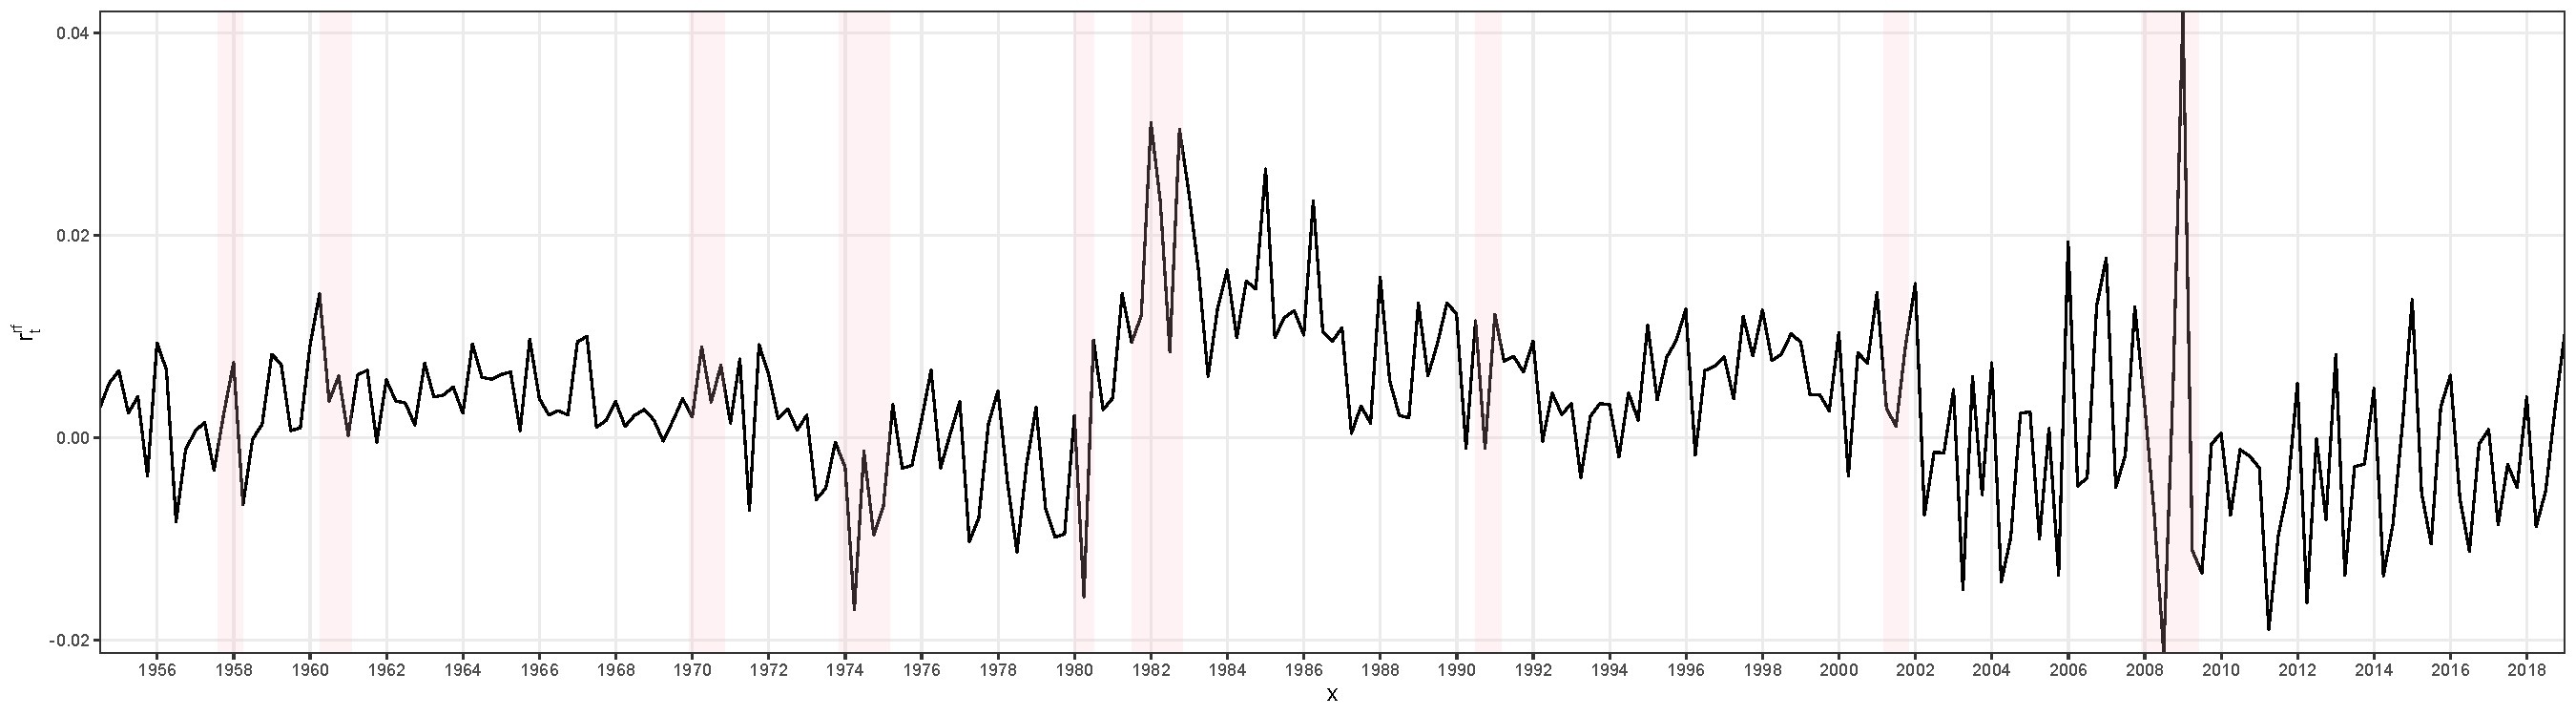
\includegraphics[width=1\linewidth]{Master_Thesis_Andreas_Kracht_Frandsen_files/figure-latex/NET-TB-tids-1} 

}

\caption[short]{A \\\raggedright Note: Blablalba.}\label{fig:NET-TB-tids}
\end{figure}

I forlængelse af beskrivelsen af det risikofrie aktiv, viser Figur \ref{fig:INF-tids} et plot over tidsserien hørende til inflationsraten.

\begin{figure}[htbp!]

{\centering 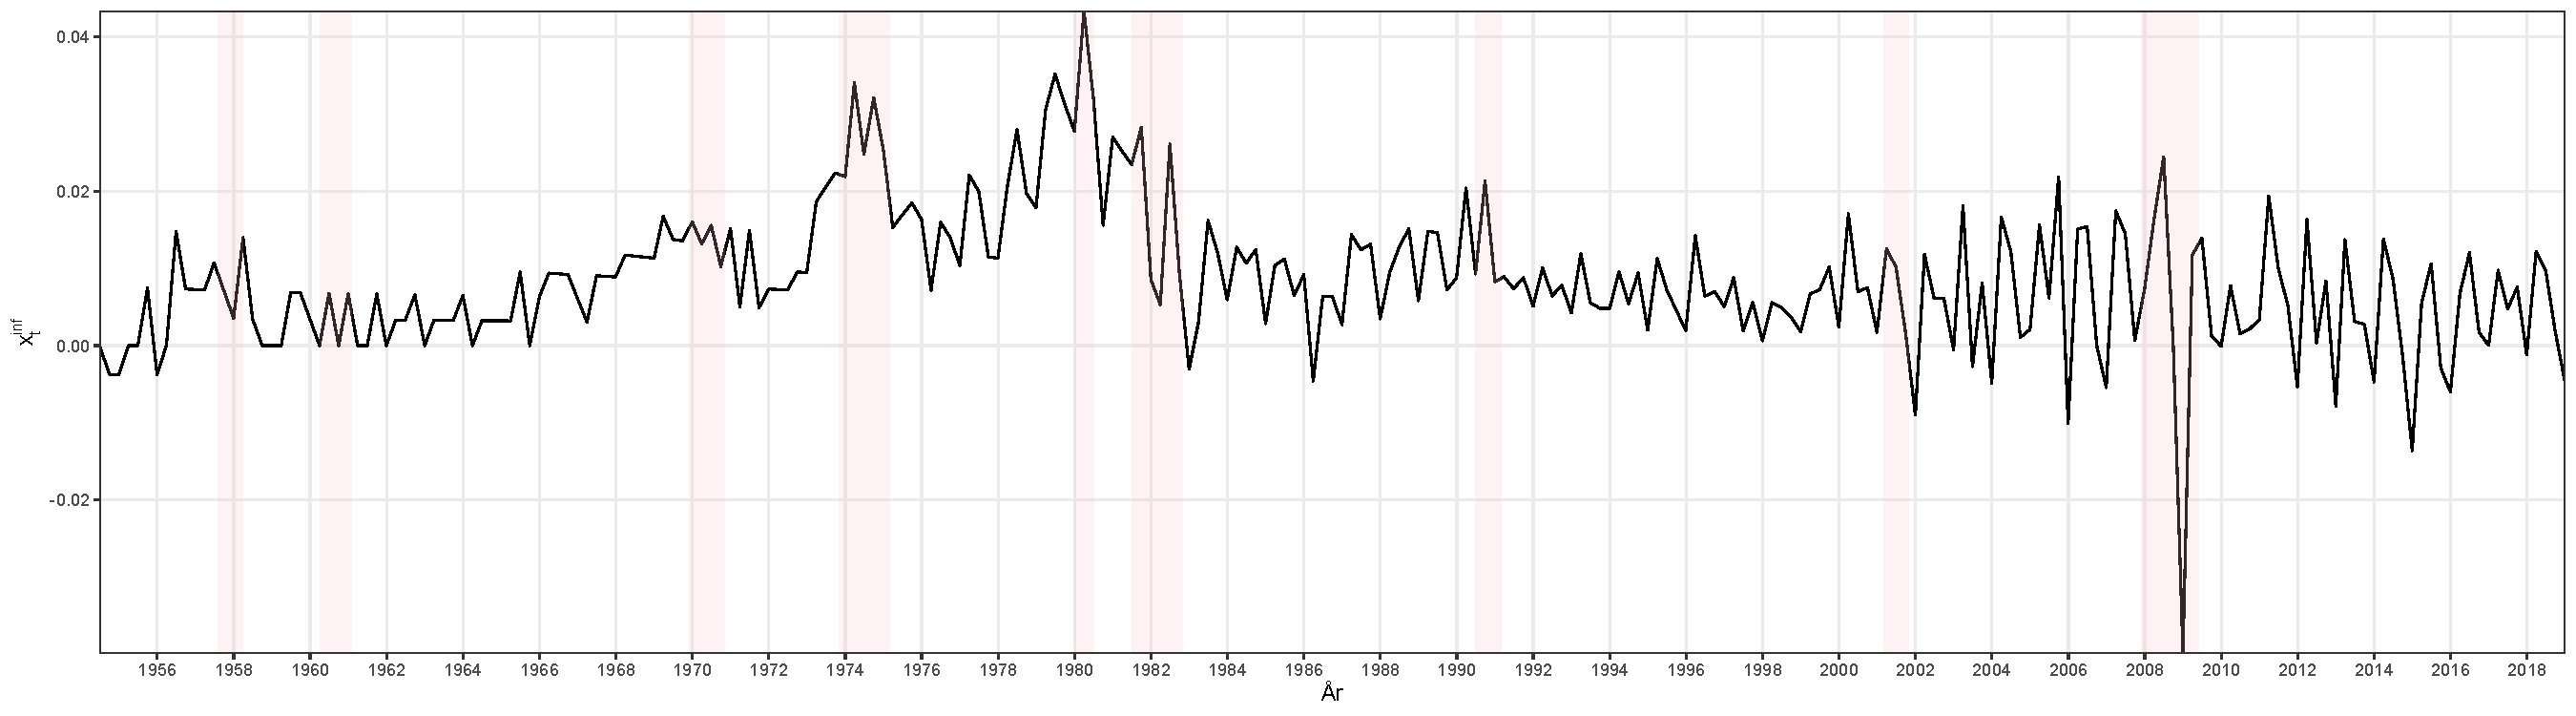
\includegraphics[width=1\linewidth]{Master_Thesis_Andreas_Kracht_Frandsen_files/figure-latex/INF-tids-1} 

}

\caption{Tidsserie af inflationsraten, målt via Consumer Price Index.}\label{fig:INF-tids}
\end{figure}

\begin{figure}[htbp!]

{\centering 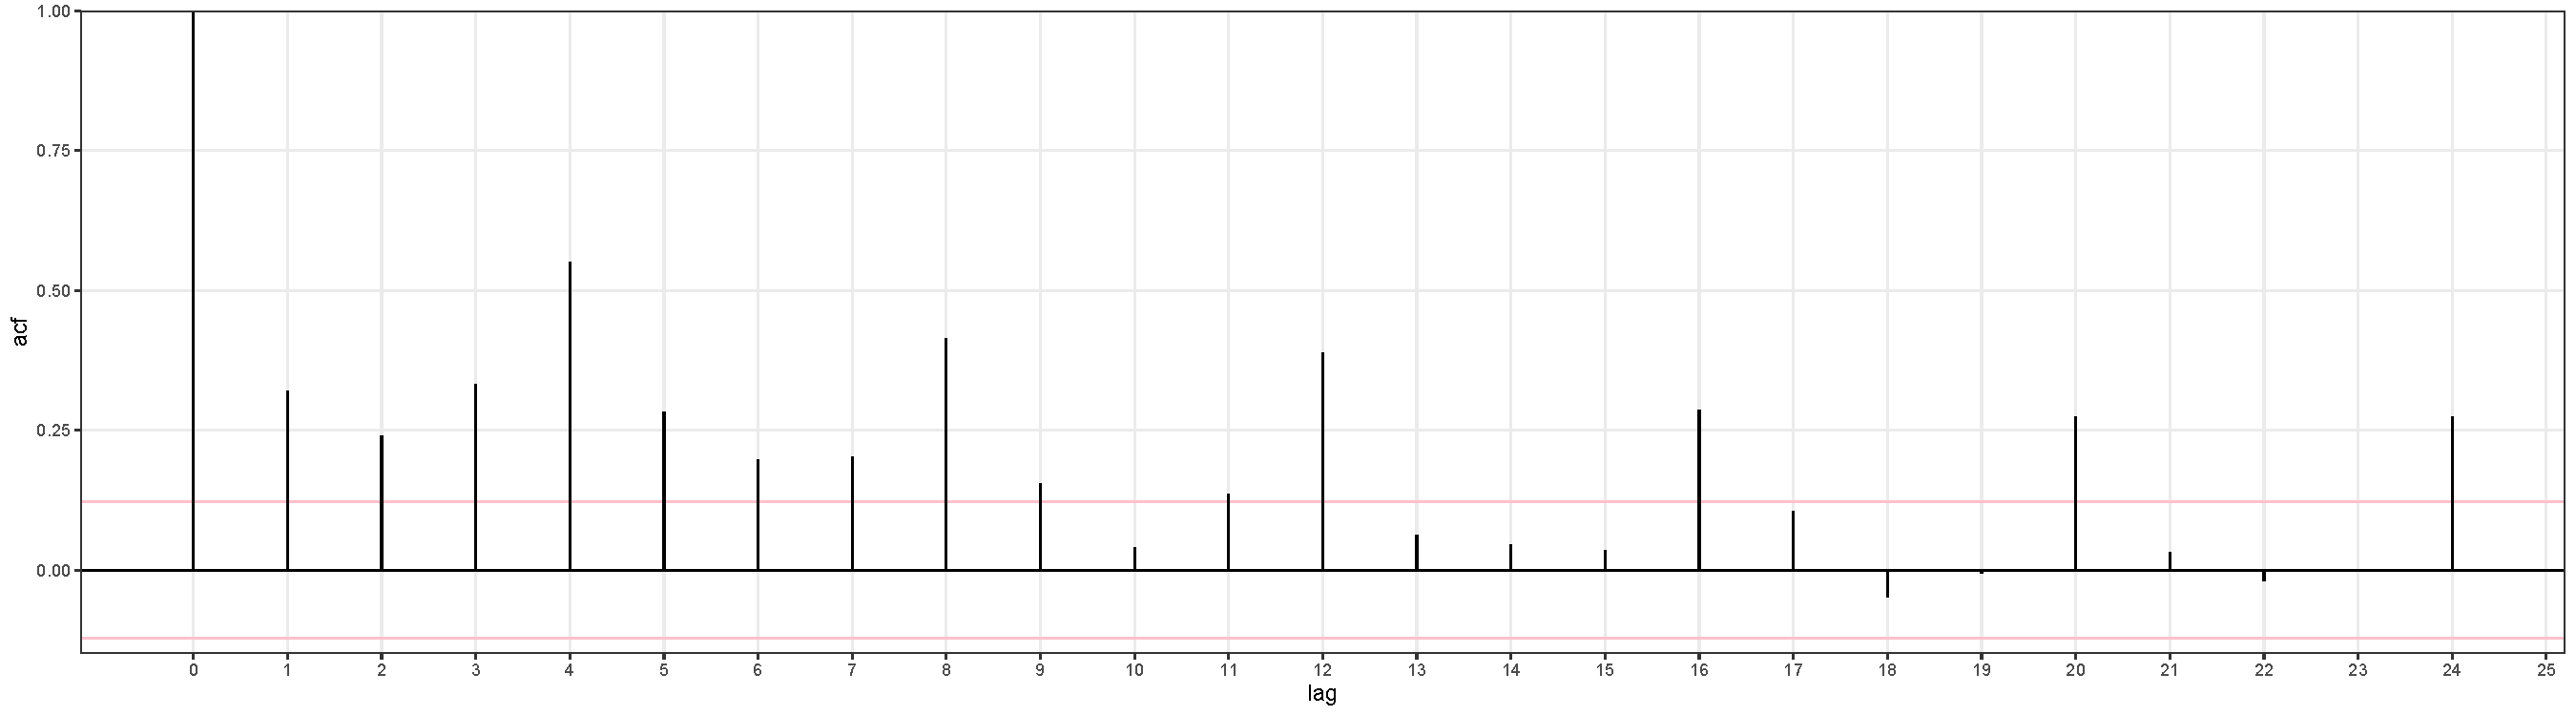
\includegraphics[width=1\linewidth]{Master_Thesis_Andreas_Kracht_Frandsen_files/figure-latex/NET-TB-AK-1} 

}

\caption{Autokorrelation af log netto renten.}\label{fig:NET-TB-AK}
\end{figure}

\begin{figure}[htbp!]

{\centering 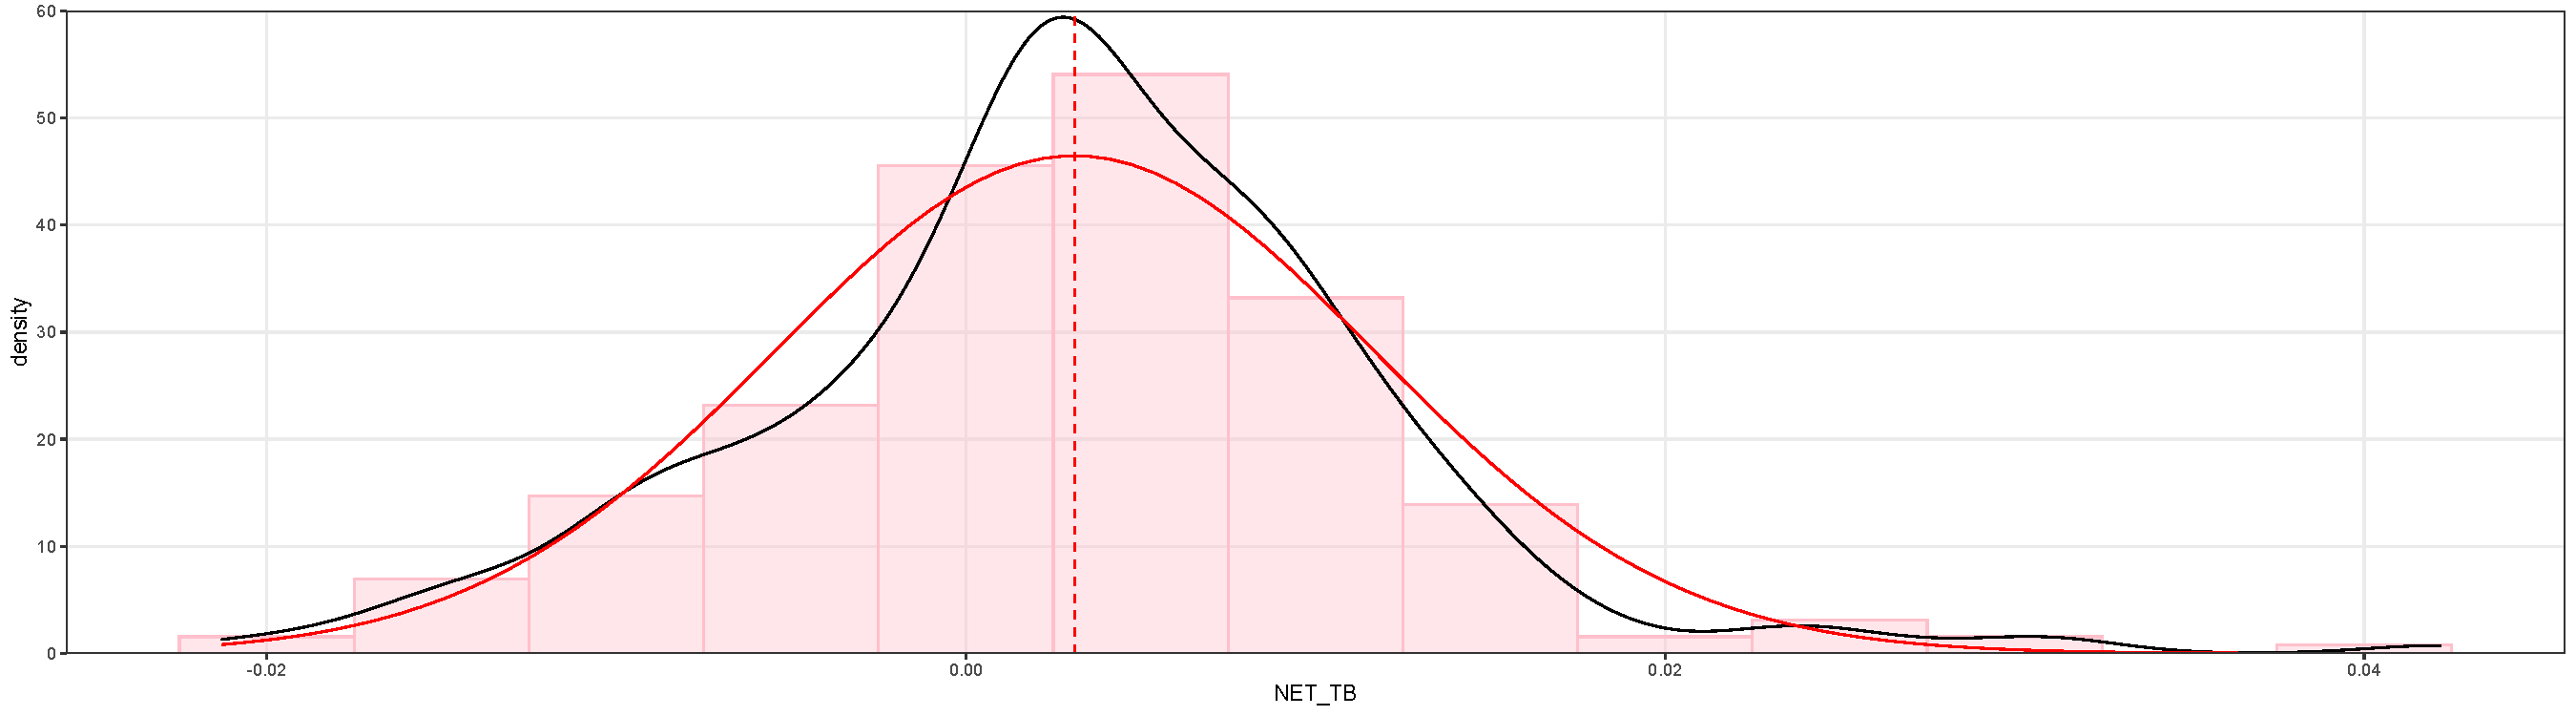
\includegraphics[width=1\linewidth]{Master_Thesis_Andreas_Kracht_Frandsen_files/figure-latex/NET-TB-HIST-1} 

}

\caption{Autokorrelation af log netto renten.}\label{fig:NET-TB-HIST}
\end{figure}

\hypertarget{dataak}{%
\subsection{\texorpdfstring{Merafkastet på aktier -- \(rx_{t+1}^{\textnormal{a}}\)}{Merafkastet på aktier -- rx\_\{t+1\}\^{}\{\textbackslash textnormal\{a\}\}}}\label{dataak}}

For aktivklassen, som skal repræsentere børshandlede aktier, benyttes et markedsværdi-vægtet afkast over et repræsentativt indeks for samtlige handlede aktier på \emph{New York Stock Exchange}, \emph{National Association of Securities Dealers Automated Quotations} og \emph{American Stock Exchange}. Det vægtede afkast er inklusiv udbytte, aktiesplits og nyemissioner for de foregående 12 måneder ledende op til kvartalet. Ved at benytte et sådant forholdsvist bredt indeks, vil delanalysen for aktier være repræsentativt for det globale aktiemarked. Derudover er det ikke kun børsnoterede amerikanskbaserede selskaber, som handles via \emph{NYSE}, \emph{NASDAQ} og \emph{AMEX}, men i stadig større grad også virksomheder uden for U.S.A. Data over afkast er fra \citep{CRSPakt} og hentet gennem \citep{WRDSakt}. Log merafkastet af aktier beregnes som det kvartalsvise log brutto aktieafkast fratrukket det kvartalsvise brutto afkast på den amerikanske 90-dages \emph{T-Bill}. Det ses at aktier har det klart højeste kvartalvise justerede merafkast på 1.7\(\%\) ift. de andre aktivklasser. Dette høje merafkast følges af en ligeledes høj relativ volatilitet på 8.3\(\%\). Historisk set har det største negative markedsudsving givet et merafkast/tab på \(-30.4\%\), mens det største positive markedsudsving har været på \(20\%\). Et histogram sammenholdt med en skævhed på -0.946 afslører moderat til høj venstreskævhed. Altså har der oftere været negative merafkast ift. positive. Kurtosis på 4.624 medører en moderat leptokurtisk fordeling med en anelse tykkere haler, og at ekstreme observationer sker oftere end normalt. Disse tal er konsistente med \citep{CampVic2003}. Figur \ref{fig:AKT-tids} viser et plot over tidsserien.

\begin{figure}[htbp!]

{\centering 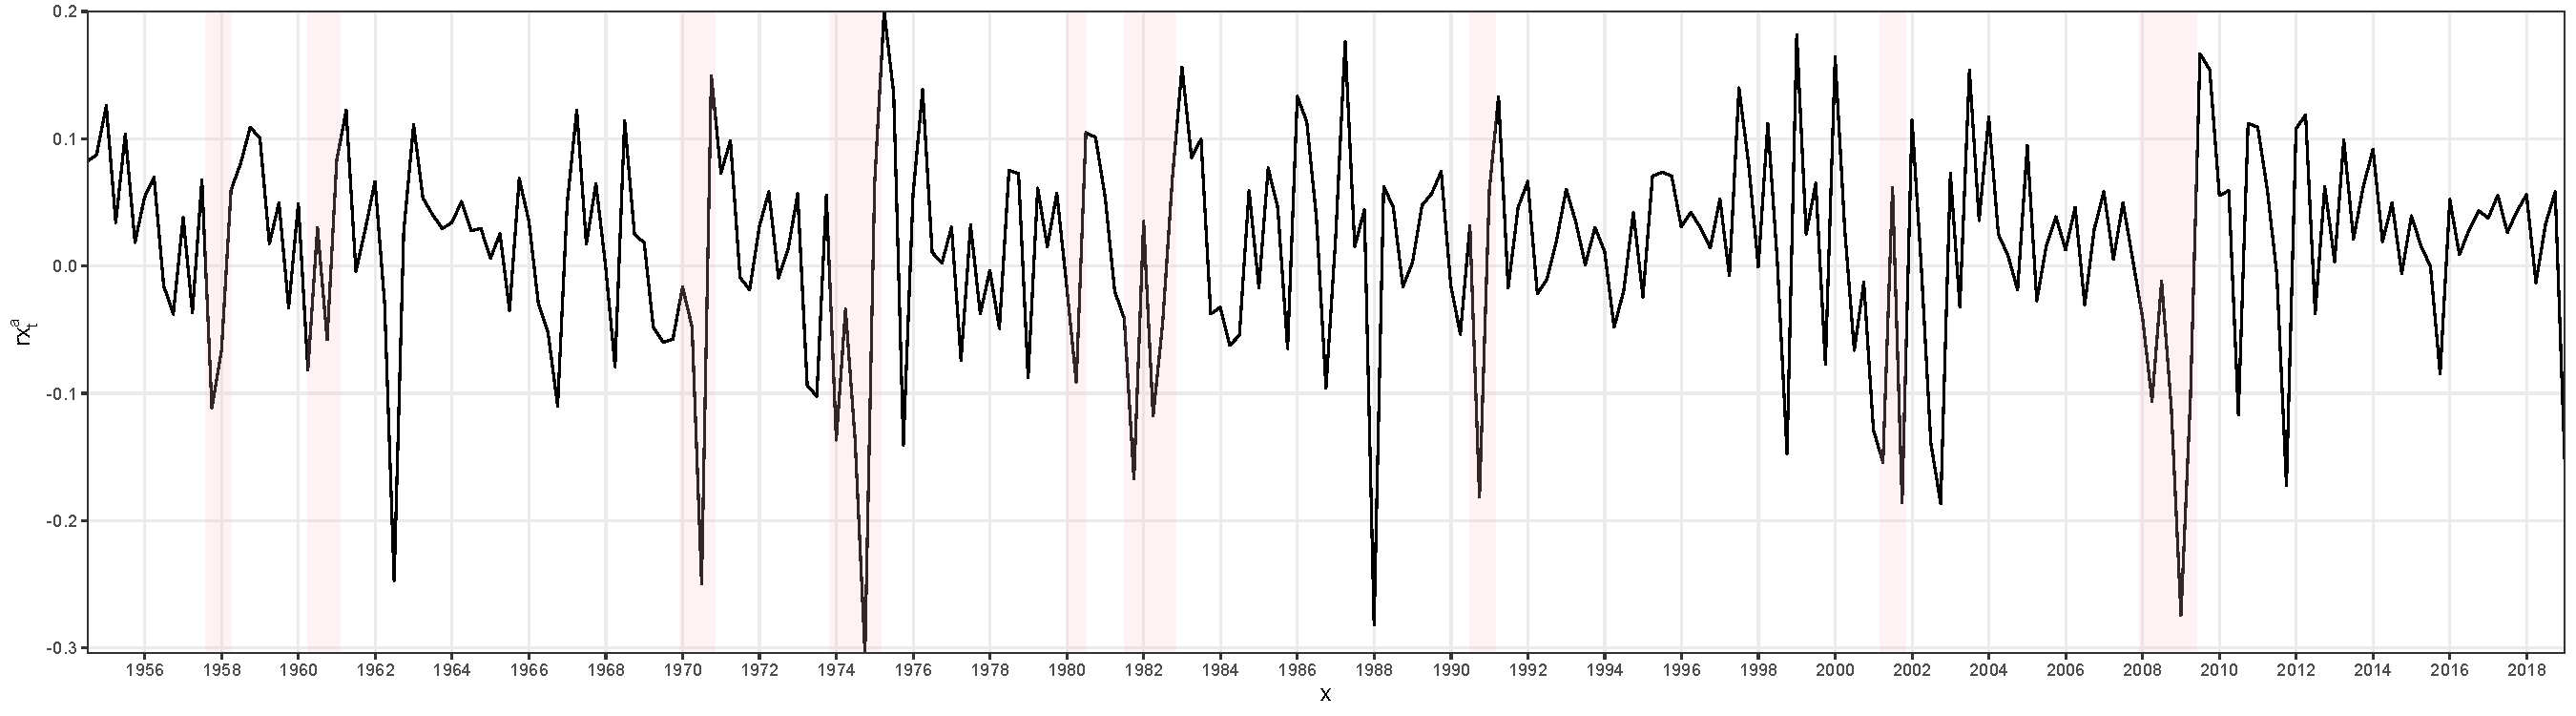
\includegraphics[width=1\linewidth]{Master_Thesis_Andreas_Kracht_Frandsen_files/figure-latex/AKT-tids-1} 

}

\caption{Tidsserie af log merafkastet af aktier.}\label{fig:AKT-tids}
\end{figure}

\begin{figure}[htbp!]

{\centering 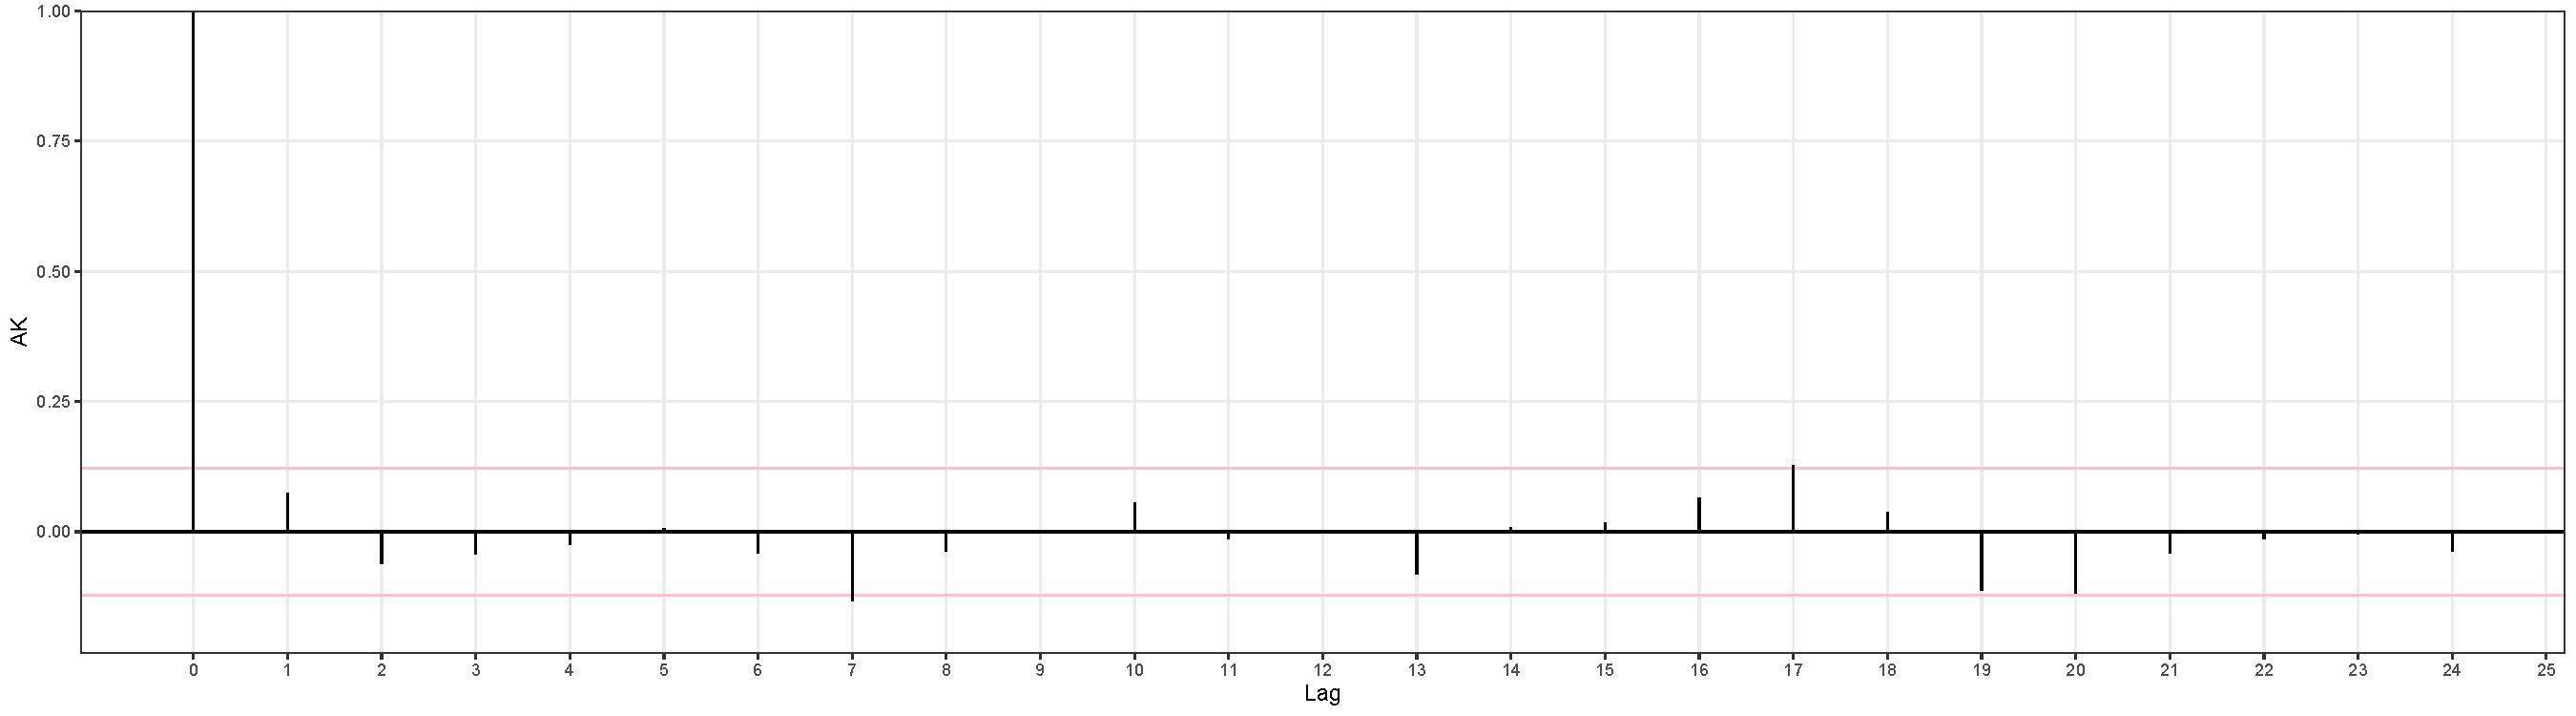
\includegraphics[width=1\linewidth]{Master_Thesis_Andreas_Kracht_Frandsen_files/figure-latex/AKT-AK-1} 

}

\caption{Autokorrelation af log merafkastet af aktier.}\label{fig:AKT-AK}
\end{figure}

\begin{figure}[htbp!]

{\centering 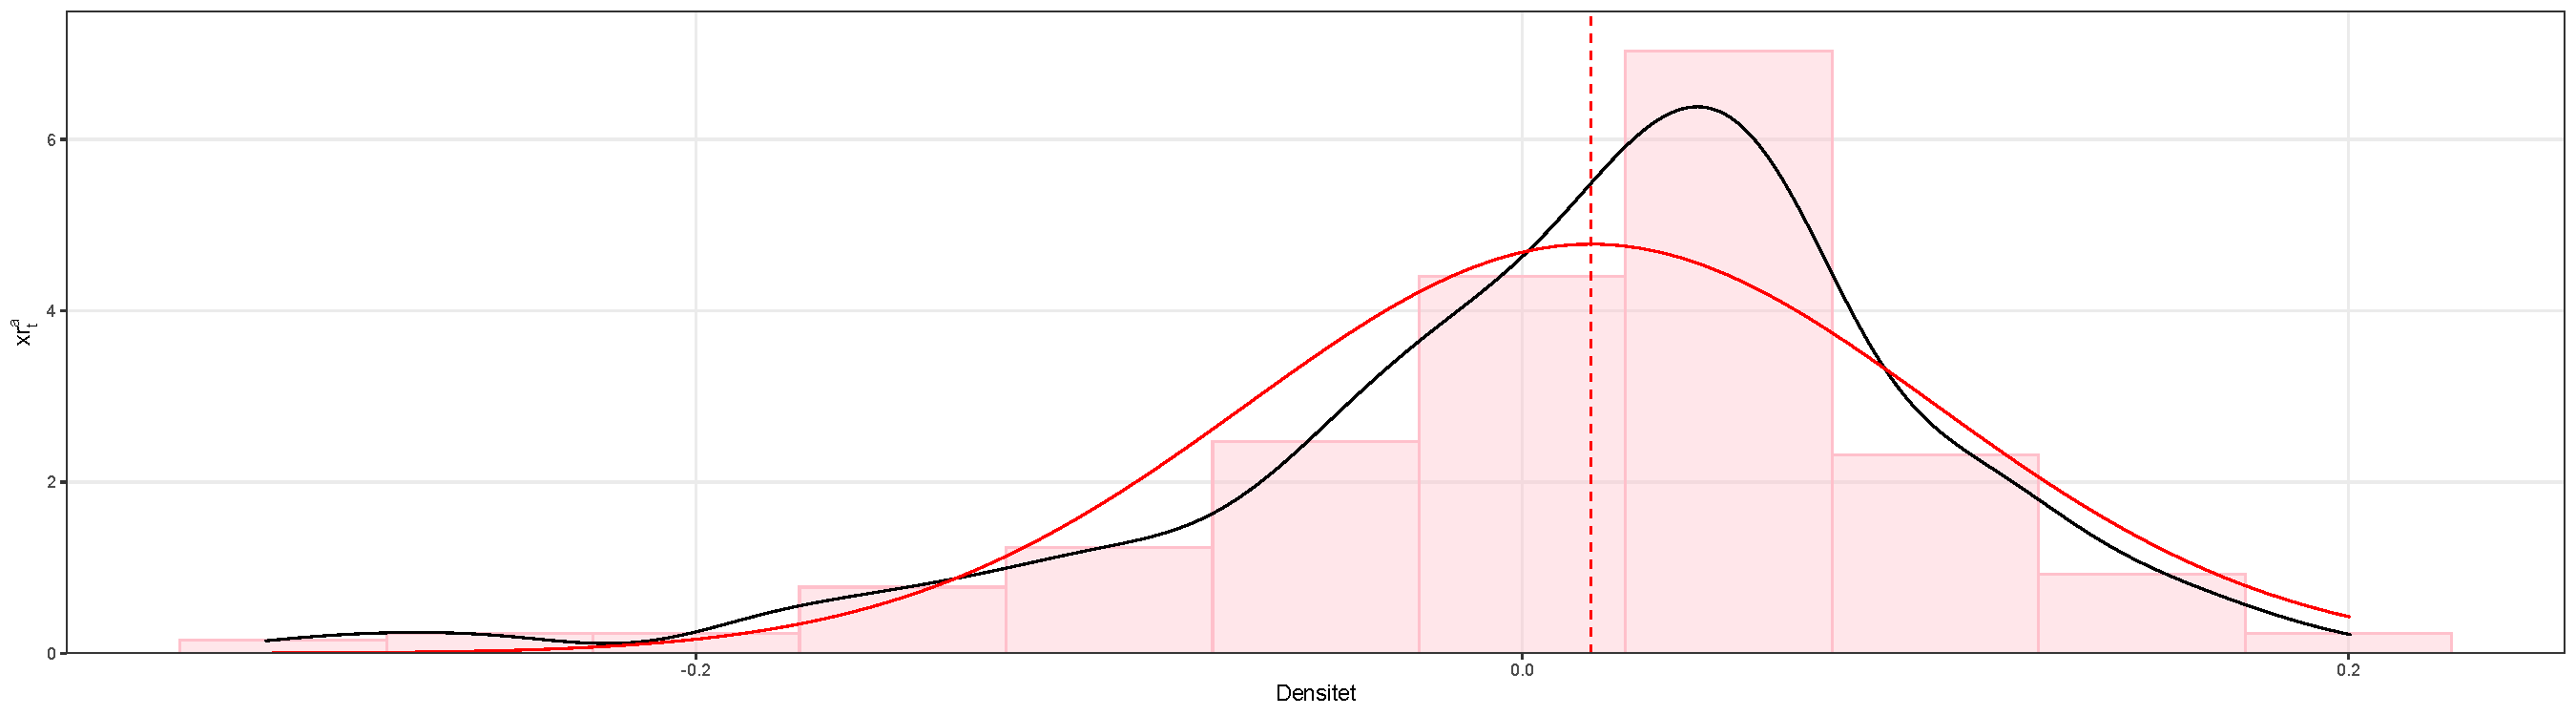
\includegraphics[width=1\linewidth]{Master_Thesis_Andreas_Kracht_Frandsen_files/figure-latex/AKT-HIST-1} 

}

\caption{Autokorrelation af log netto renten.}\label{fig:AKT-HIST}
\end{figure}

\hypertarget{merafkastet-puxe5-statsobligationer-rx_t1textnormals}{%
\subsection{\texorpdfstring{Merafkastet på statsobligationer -- \(rx_{t+1}^{\textnormal{s}}\)}{Merafkastet på statsobligationer -- rx\_\{t+1\}\^{}\{\textbackslash textnormal\{s\}\}}}\label{merafkastet-puxe5-statsobligationer-rx_t1textnormals}}

Statsobligationer er gældsinstrumenter udstedt af staten i det respektive udstedelsesland, de har til formål at finansiere offentlige udgifter og anses også for at være en substitution for skatter. Siden udstedelsen sker af staten, antages det ofte, at statsobligationer er relativt mindre risikobærende and aktier. Undertiden betegnes statsobligationer fra visse ilande som et \emph{safe haven} for investorer. Eksempelvis har den danske stat pt.~en kreditvurdering på AAA, Aaa, AAA af hhv. \emph{Standard \& Poor's}, \emph{Moody's} og \emph{Fitch}, \citep{TradingEconomics2020}. Til formålet at repræsentere afkastet på statsobligationer anvendes derfor den 10-årige amerikanske statsobligation med konstant løbetid. Data over afkast er fra \citep{CRSPt90} og hentet gennem \citep{WRDSt90}. Log merafkastet af statsobligationener beregnes som det kvartalsvise log brutto afkast fratrukket det kvartalsvise brutto afkast på den amerikanske 90-dages \emph{T-Bill}. merafkastet har et justeret kvartalsvist afkast på 0.3\(\%\) med en kvartalsvis volatilitet på 3.8\(\%\). Statsobligationen har den laveste \emph{Sharpe Ratio} af de tre aktivklasser, hvilket også er forventeligt. Med en skævhed på 0.451 og kurtosis på 3.405 haves en forholdsvis symmetrisk fordeling, men med en anelse tykkere haler. Disse tal er konsistente med \citep{CampVic2003}. Figur \ref{fig:S-OBL-tids} viser et plot over tidsserien.

\begin{figure}[htbp!]

{\centering 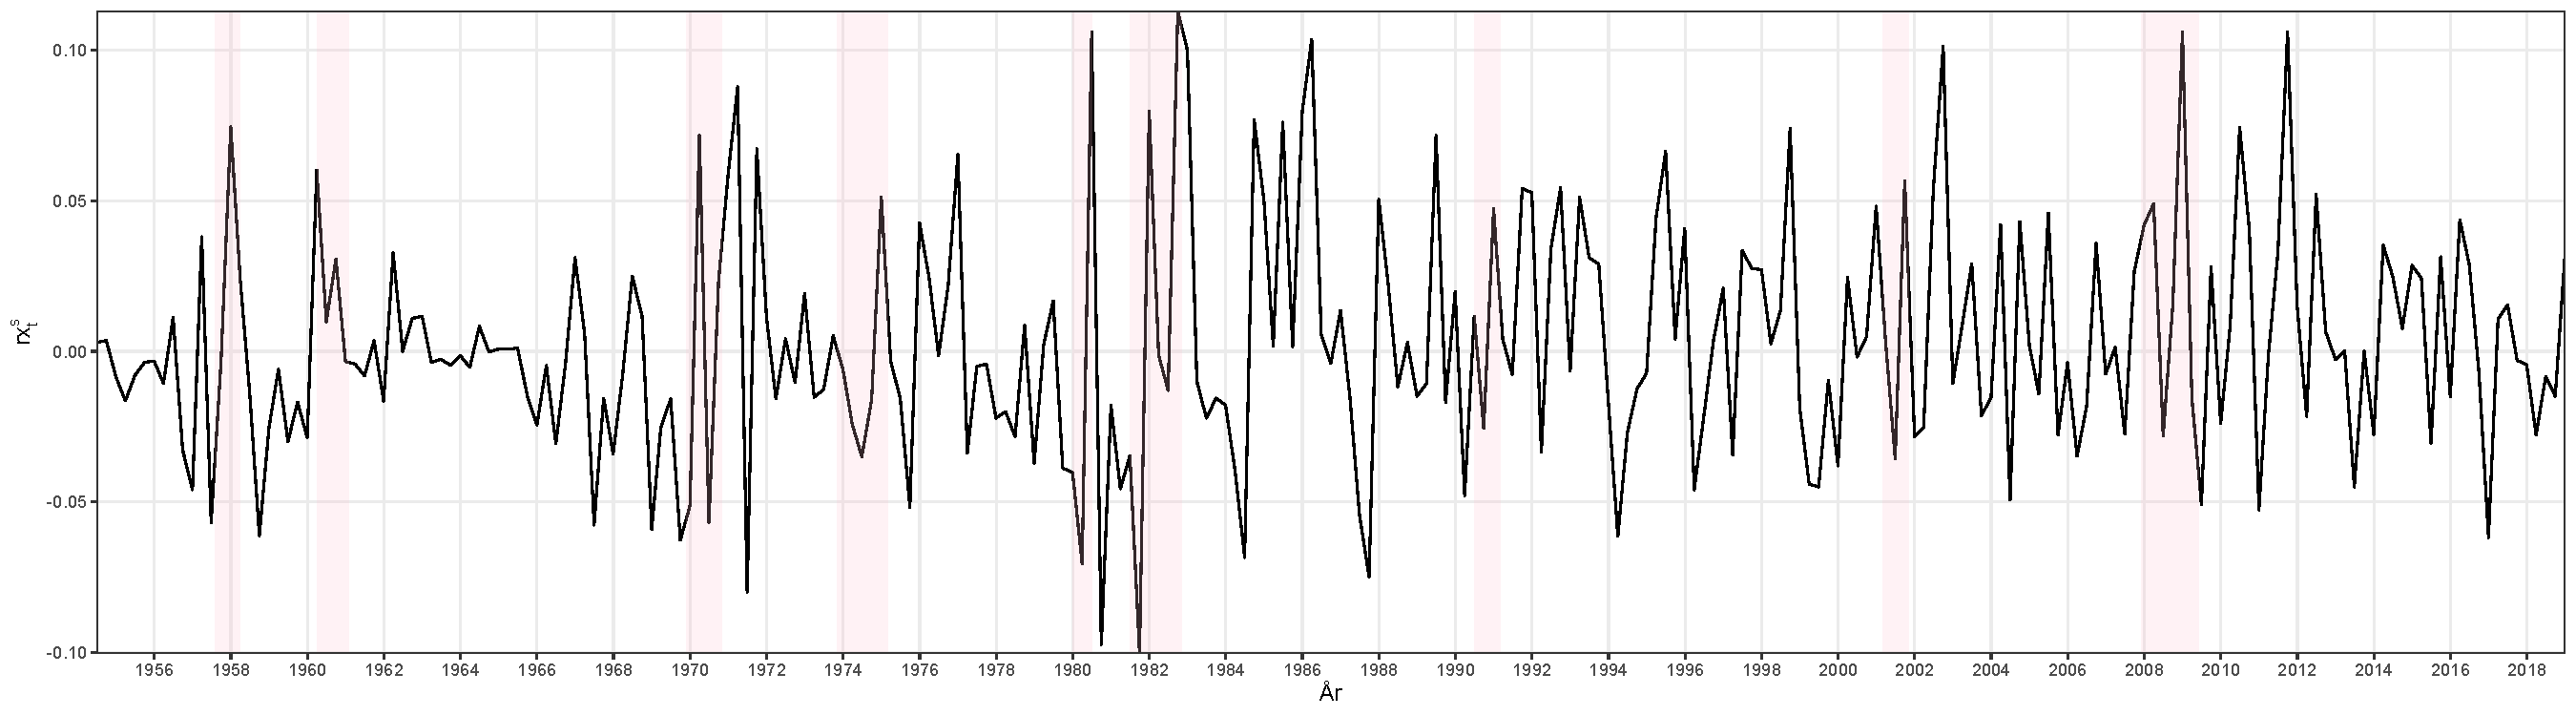
\includegraphics[width=1\linewidth]{Master_Thesis_Andreas_Kracht_Frandsen_files/figure-latex/S-OBL-tids-1} 

}

\caption{Tidsserie af log  merafkastet på statsobligationer.}\label{fig:S-OBL-tids}
\end{figure}

\begin{figure}[htbp!]

{\centering 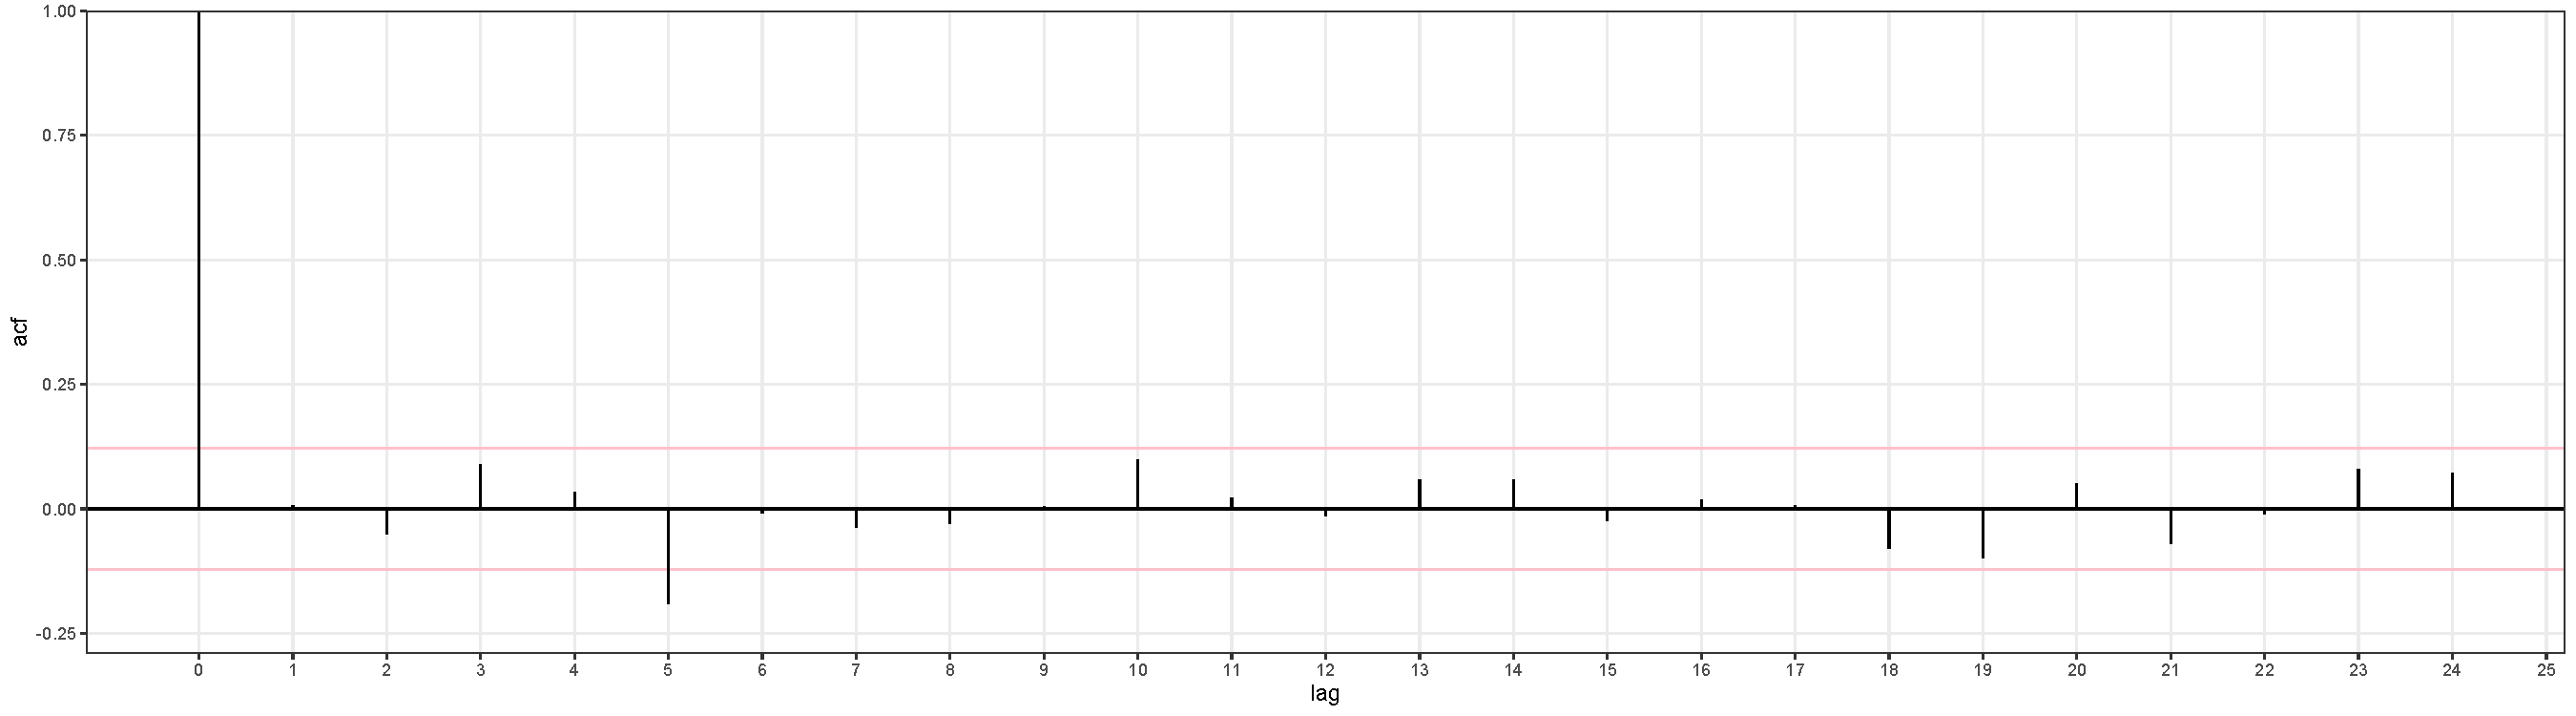
\includegraphics[width=1\linewidth]{Master_Thesis_Andreas_Kracht_Frandsen_files/figure-latex/S-OBL-AK-1} 

}

\caption{Autokorrelation af log merafkastet af statsobligationer.}\label{fig:S-OBL-AK}
\end{figure}

\begin{figure}[htbp!]

{\centering 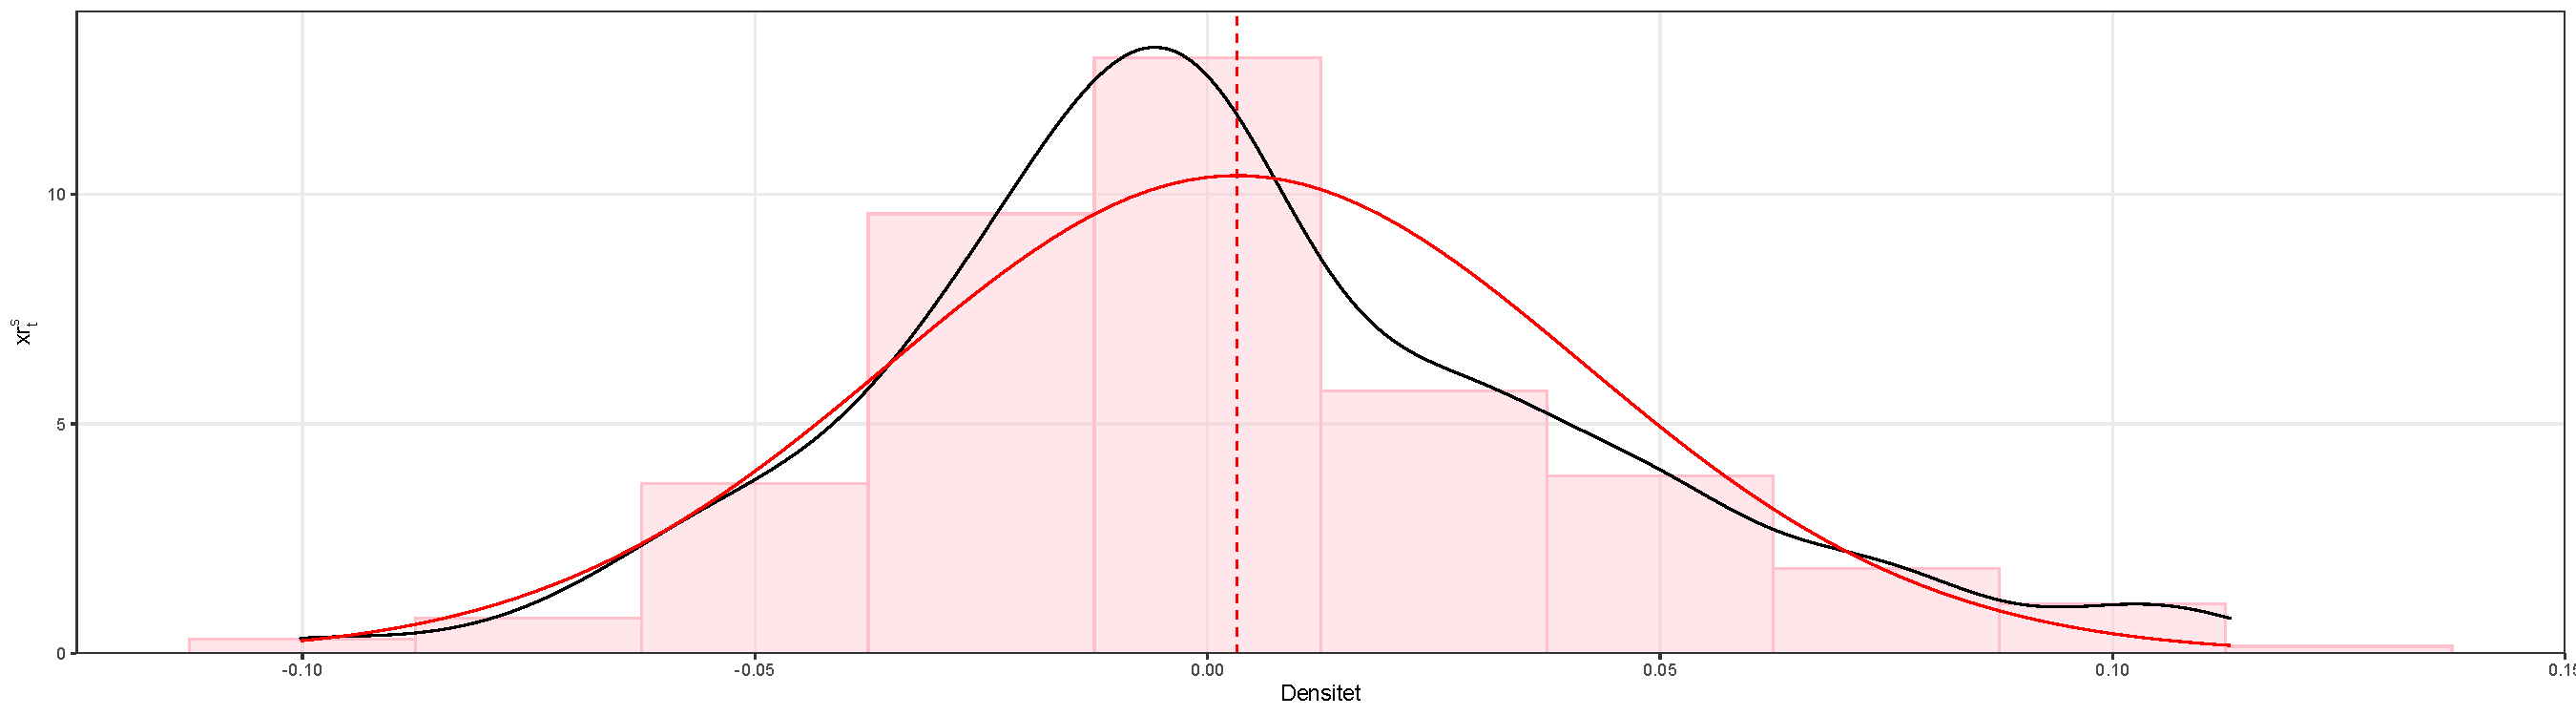
\includegraphics[width=1\linewidth]{Master_Thesis_Andreas_Kracht_Frandsen_files/figure-latex/S-OBL-HIST-1} 

}

\caption{Autokorrelation af log netto renten.}\label{fig:S-OBL-HIST}
\end{figure}

\hypertarget{merafkastet-puxe5-virksomhedsobligationer-rx_t1textnormalv}{%
\subsection{\texorpdfstring{Merafkastet på virksomhedsobligationer -- \(rx_{t+1}^{\textnormal{v}}\)}{Merafkastet på virksomhedsobligationer -- rx\_\{t+1\}\^{}\{\textbackslash textnormal\{v\}\}}}\label{merafkastet-puxe5-virksomhedsobligationer-rx_t1textnormalv}}

På samme vis som stater kan finansiere deres aktiviteter via statsobligationer, kan virksomheder udstede gæld via obligationer, hvis formål er at finansiere fremtidige investeringer og/eller projekter. Sikkerheden bag en virksomhedsobligation afhænger af virksomhedens betalingsevne. Af og til sætter virksomheden fysiske aktiver som kollateral for obligationerne i tilfælde af konkurser. Ift. statsobligationer bærer virksomhedsobligationer på en langt større risiko givet kreditrisikoen i virksomheden og/eller markedet. For at påtage sig denne risiko, forlanger investorerne derfor en højere præmie i form af en højere rente tilhørende virksomhedsobligationerne. For at repræsentere virksomhedsobligationer anvendes en indeksserie af virksomhedsobligationer med lang løbetid. Data er fra \citep{Ibbotson2019} og hentet via \citep{Goyal2007}\footnote{Mere specifickt via \emph{Amit Goyals} hjemmeside, hvor der findes en opdateret version af dataet, som der benyttes i artiklen, se evt. \citep{Goyal2020}.}. Det specifikke grundlag for tidsserien er tvetydigt, men \citep{Ibbotson2019} skriver følgende.

\begin{center}
\textit{A corporate bond series with a long maturity is used to describe fixed-income securities that contain risk of default.}
\end{center}

Log merafkastet af virksomhedsobligationenerne beregnes som det kvartalsvise log brutto afkast fratrukket det kvartalsvise brutto afkast på den amerikanske 90-dages \emph{T-Bill}. Som forventet ses den højere afkastpræmie med et justeret kvartalsvist afkast på 0.5\(\%\) og en tilhørende volatilitet på 4.7\(\%\), som investoren får, for at påtage sig den ekstra kreditrisiko. Afkastfordelingen anses som værende relativt mest symmetrisk ift. de andre aktivklasser, hvilket også ses i en skævhedsværdi på 0.216. Med en kurtosis på mere end \(3\), har fordelingen tykkere haler og med mere masse centralt i fordelingen. Det bemærkes ligeledes at virksomhedsobligationer har haft de største positive markedsudsving af de tre aktivklasser med et positivt afkast på \(20.8 \%\). Figur \ref{fig:V-OBL-tids} viser et plot over tidsserien.

\begin{figure}[htbp!]

{\centering 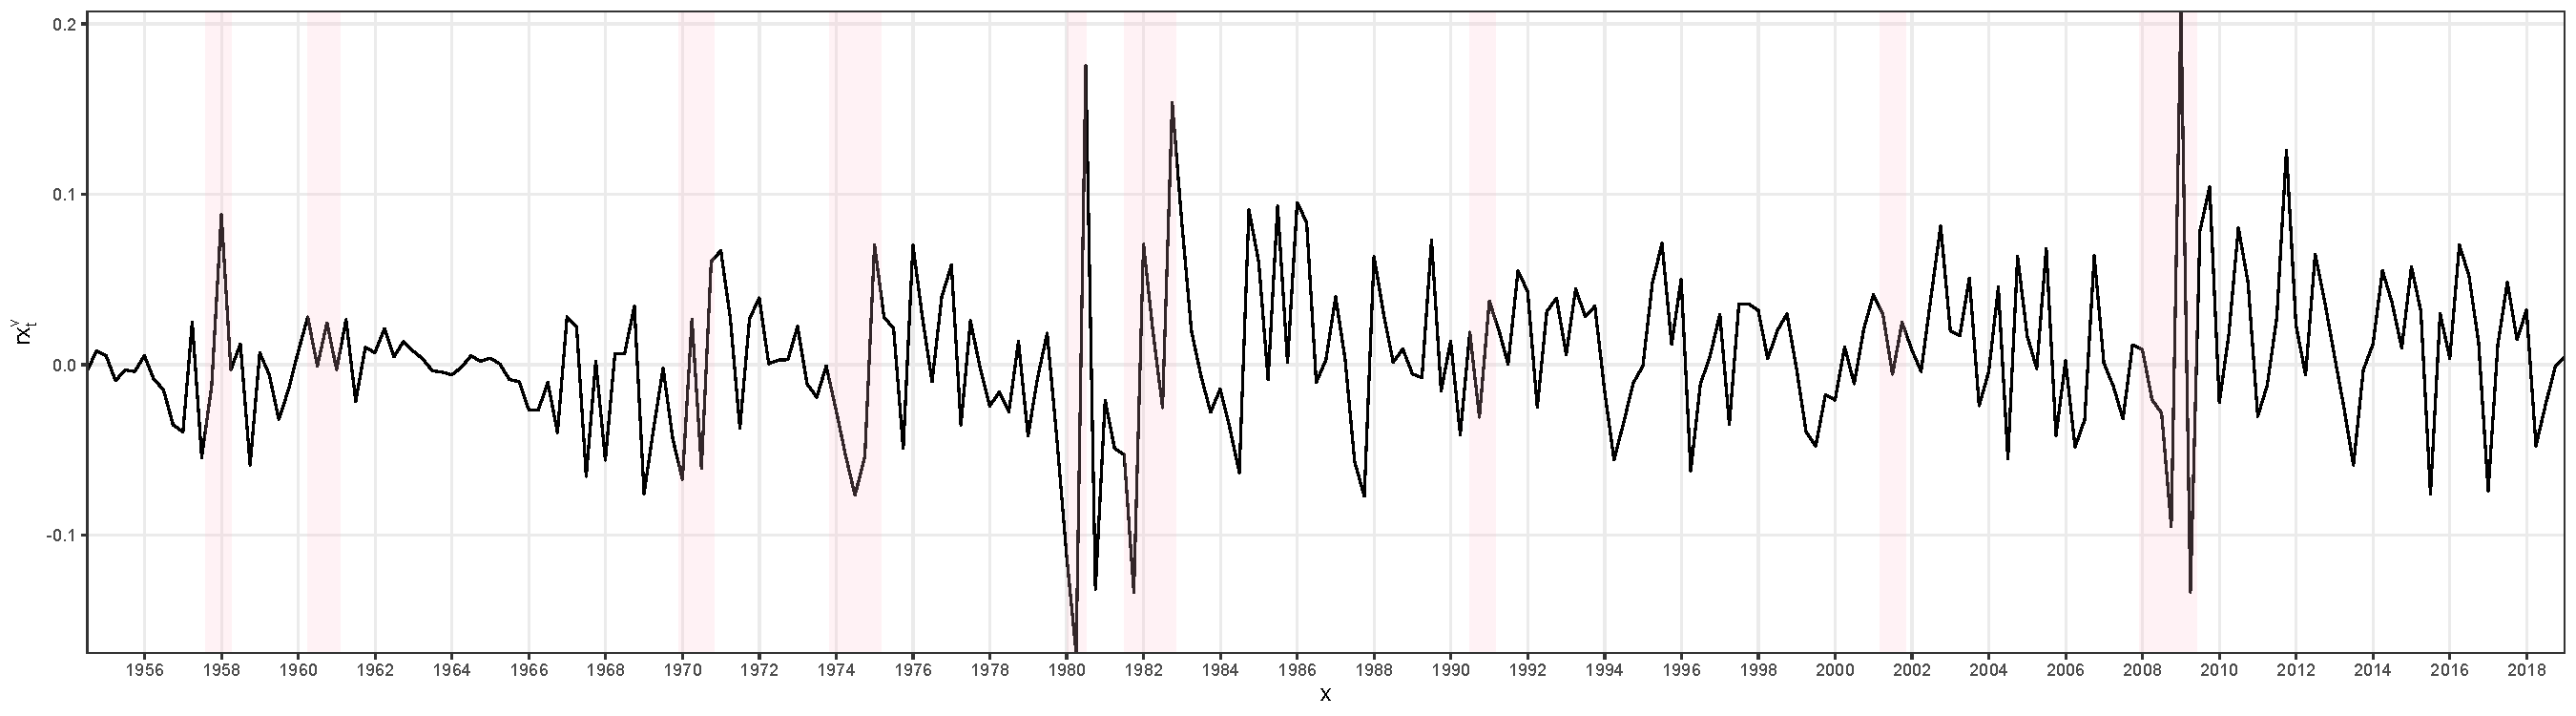
\includegraphics[width=1\linewidth]{Master_Thesis_Andreas_Kracht_Frandsen_files/figure-latex/V-OBL-tids-1} 

}

\caption{Tidsserie af log  merafkastet på virksomhedsobligationer.}\label{fig:V-OBL-tids}
\end{figure}

\begin{figure}[htbp!]

{\centering 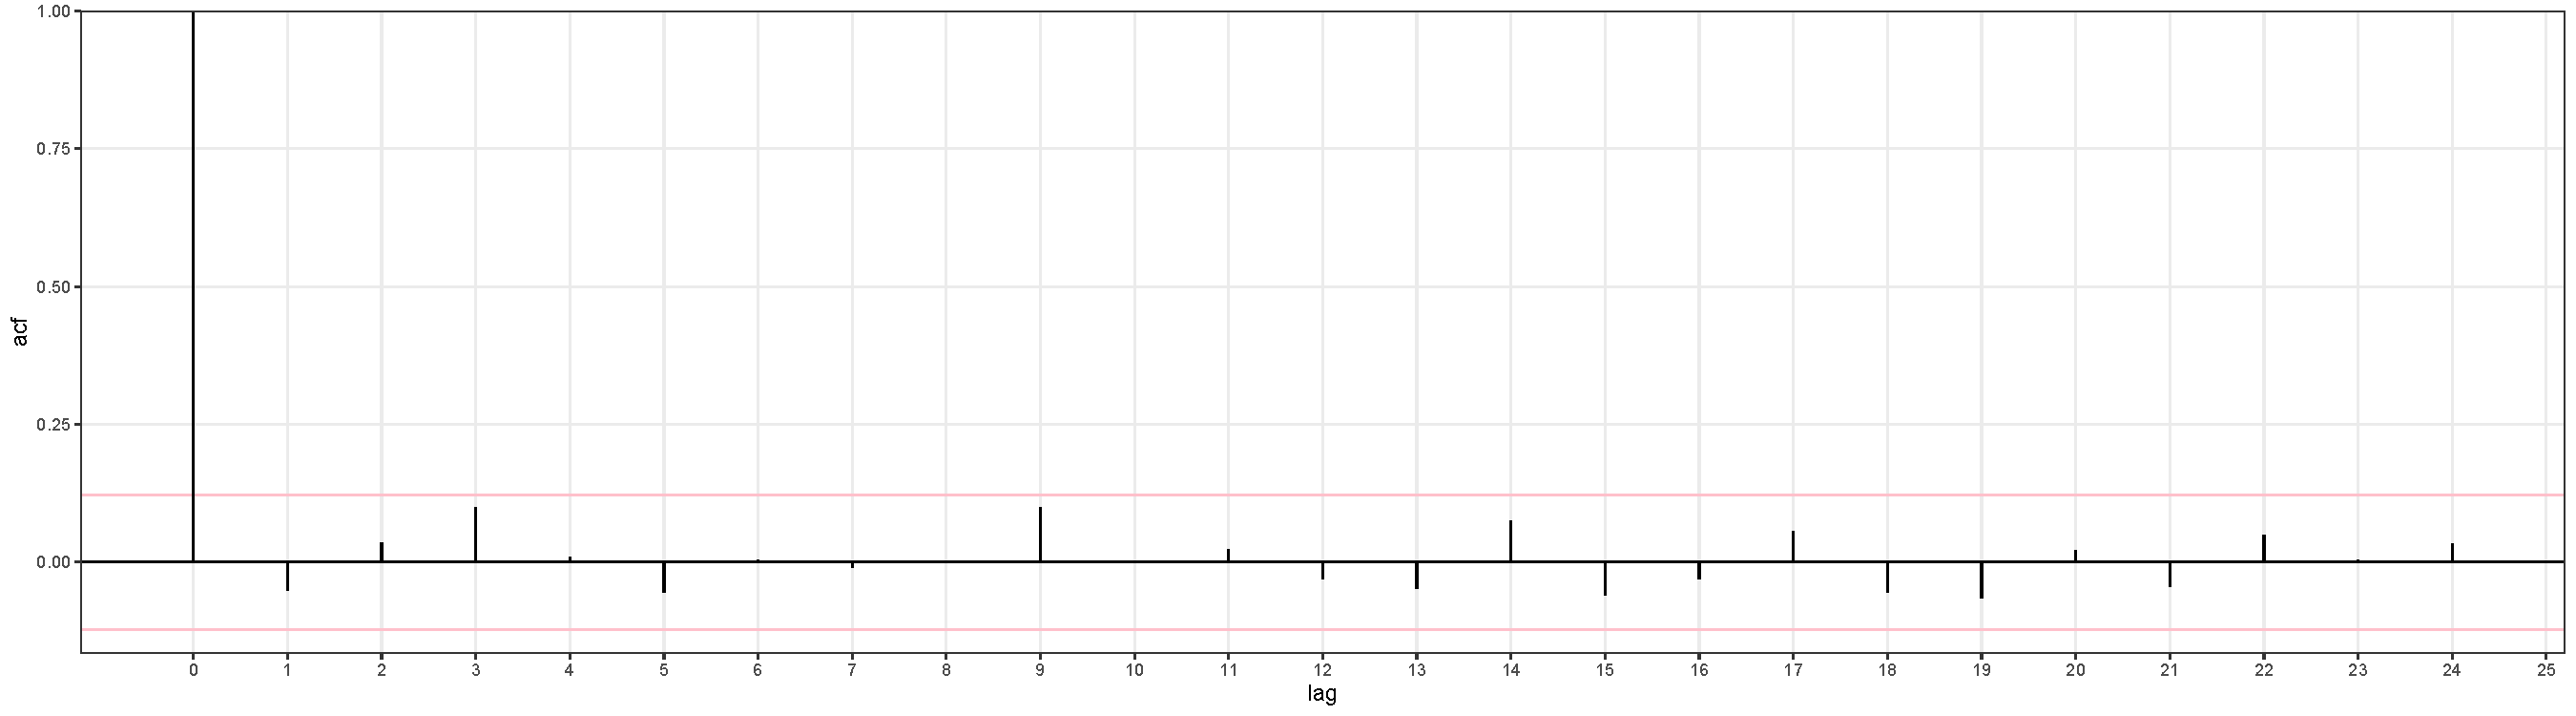
\includegraphics[width=1\linewidth]{Master_Thesis_Andreas_Kracht_Frandsen_files/figure-latex/V-OBL-AK-1} 

}

\caption{Autokorrelation af log merafkastet af virksomhedsobligationer.}\label{fig:V-OBL-AK}
\end{figure}

\begin{figure}[htbp!]

{\centering 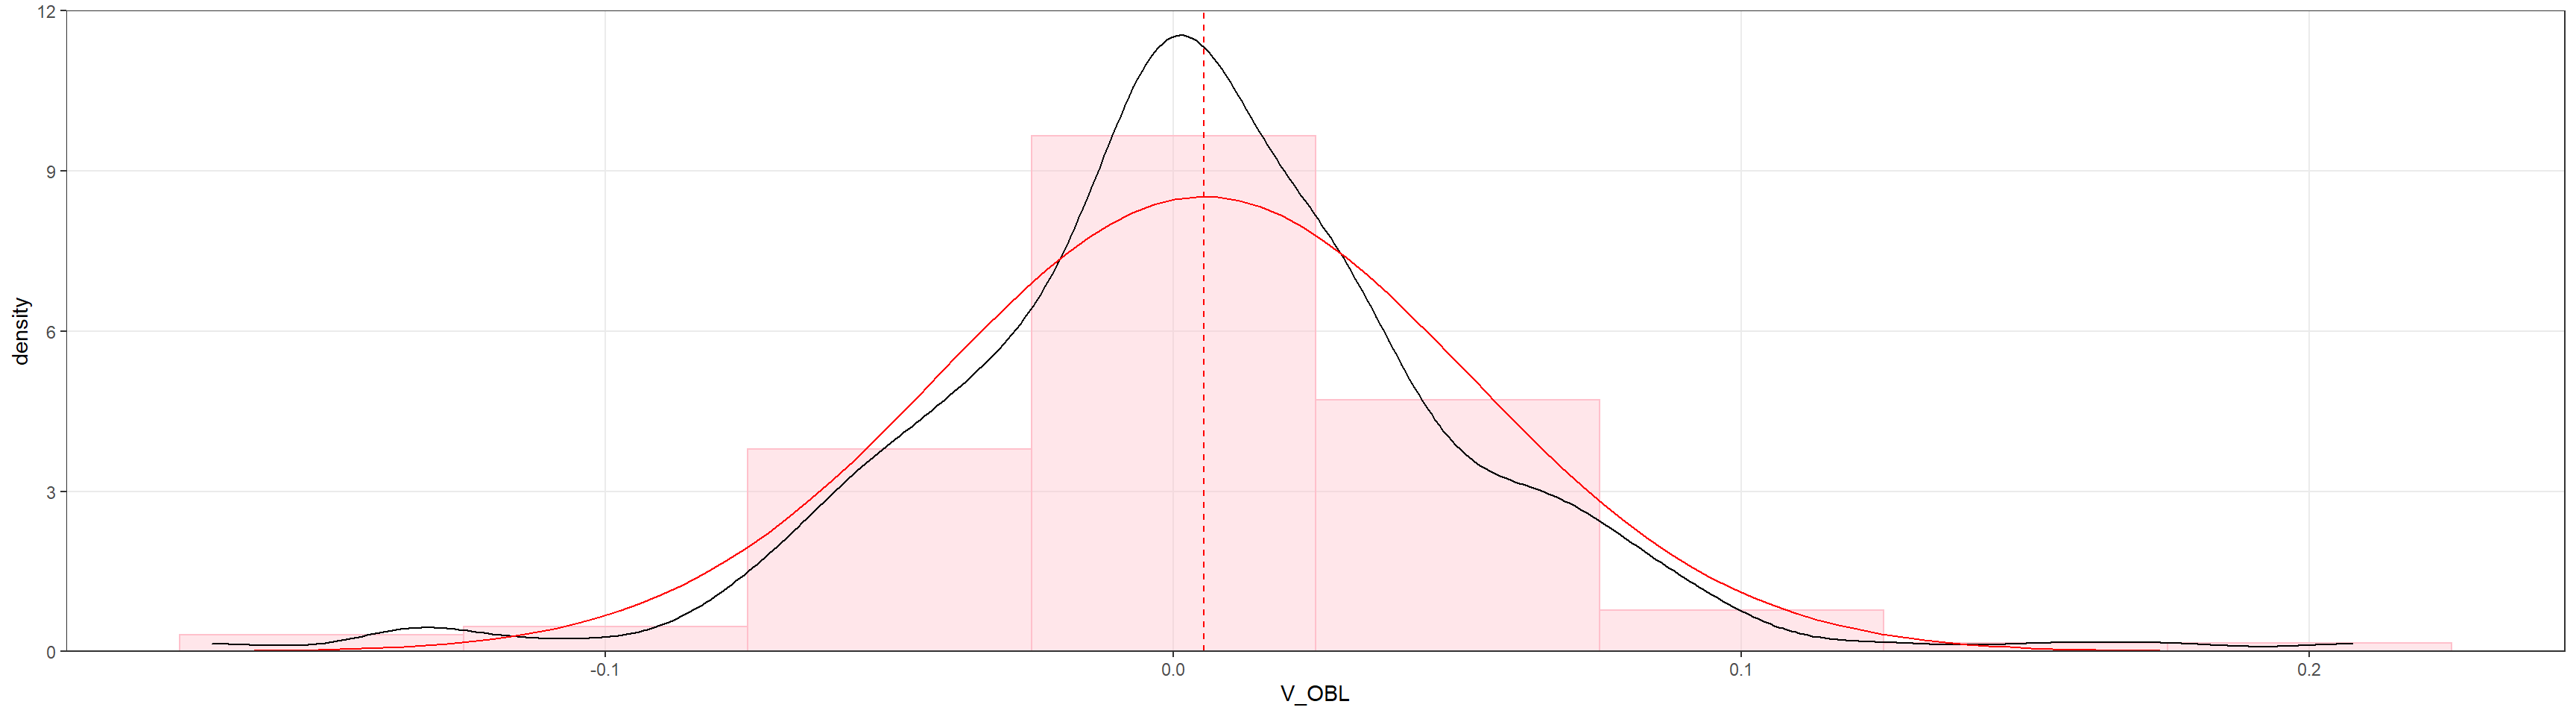
\includegraphics[width=1\linewidth]{Master_Thesis_Andreas_Kracht_Frandsen_files/figure-latex/V-OBL-HIST-1} 

}

\caption{Autokorrelation af log netto renten.}\label{fig:V-OBL-HIST}
\end{figure}

Tabel \ref{tab:DES-AKTIVKLASSE} opsummerer ovenstående beskrivende statistik for de fire aktivkasser.



\begin{landscape}
\begin{table}[!h]

\caption{\label{tab:DES-AKTIVKLASSE}Beskrivende statistik for de fire aktivklasser.}
\centering
\begin{threeparttable}
\begin{tabular}[t]{lrrrrrrrrrrr}
\toprule
  & Middelværdi & Standard afvigelse & Sharpe Ratio & Skævhed & Kurtosis & Minimum & $25 \%$ & Median & $75 \%$ & Maksimum & AK(1)\\
\midrule
\rowcolor{gray!6}  $r_t^{\text{rf}}$ & 0.003 & 0.009 &  & 0.362 & 5.016 & -0.021 & -0.001 & 0.003 & 0.008 & 0.042 & 0.320\\
$rx_t^{\text{a}}$ & 0.017 & 0.083 & 0.199 & -0.946 & 4.624 & -0.304 & -0.028 & 0.029 & 0.062 & 0.200 & 0.075\\
\rowcolor{gray!6}  $rx_t^{\text{s}}$ & 0.003 & 0.038 & 0.084 & 0.451 & 3.405 & -0.100 & -0.021 & -0.003 & 0.025 & 0.113 & 0.007\\
$rx_t^{\text{v}}$ & 0.005 & 0.047 & 0.114 & 0.216 & 5.588 & -0.169 & -0.021 & 0.003 & 0.028 & 0.208 & -0.051\\
\bottomrule
\end{tabular}
\begin{tablenotes}
\item \textit{Note: } 
\item \textit{Denne tabel rapporterer kvartalsvis beskrivende statistik for aktivklasserne: det risikofrie aktiv, merafkastet på aktier, merafkastet på statsobligationer og merafkastet på virksomhedsobligationer. Dette gøres ud fra $259$ kvartalvise observationer, som spænder over kvartalerne fra 2. kvartal 1954 til 4. kvartal 2018. Middelværdien er justeret for alle aktivklasser.}
\end{tablenotes}
\end{threeparttable}
\end{table}

\begin{table}[!h]

\caption{\label{tab:JB-AKTIVKLASSE}Jarque-Bera test.}
\centering
\begin{threeparttable}
\begin{tabular}[t]{lrr}
\toprule
  & Teststørrelse & $p$-værdi\\
\midrule
\rowcolor{gray!6}  $r_t^{\text{rf}}$ & 49.509 & 0.000\\
$rx_t^{\text{a}}$ & 67.131 & 0.000\\
\rowcolor{gray!6}  $rx_t^{\text{s}}$ & 10.545 & 0.005\\
$rx_t^{\text{v}}$ & 74.307 & 0.000\\
\bottomrule
\end{tabular}
\begin{tablenotes}
\item \textit{Note: } 
\item \textit{Denne tabel rapporterer Jarque-Beta teststørrelser og $p$-værdier for aktivklasserne: det risikofrie aktiv, merafkastet på aktier, merafkastet på statsobligationer og merafkastet på virksomhedsobligationer, \citep{Jarque1980}. Dette gøres ud fra $259$ kvartalvise observationer, som spænder over kvartalerne fra 2. kvartal 1954 til 4. kvartal 2018.}
\end{tablenotes}
\end{threeparttable}
\end{table}
\end{landscape}

\hypertarget{pvariable}{%
\section{Prædiktionsvariable}\label{pvariable}}

Denne sektion har til formål at beskrive datagrundlaget for prædiktionsvariablene, som først blev beskrevet i Sektion ??. Disse variable består af en række finansielle indikatorer: \emph{Dividend-Price Ratio}, \emph{Price-Earnings Ratio}, \emph{Book-to-market Ratio}, \emph{High Minus Low}, \emph{Small Minus Big}, og variansen af aktieafkast. Derudover haves rentestruktursprædiktionsvariable: den nominelle rente, \emph{Term Spread}, \emph{Yield Spread}, \emph{Credit Spread} og \emph{Default Spread}. Én makroøkonomisk variabel udgør den sidste prædiktionsvariabel: \emph{Federal Funds Rate}. Udover beskrivelsen og begrundelsen beregningsmetoden for hver variabel, vil den tilhørende beskrivende statistik for hver variabel belyses.

\hypertarget{dividend-price-ratio-x_ttextdp}{%
\subsection{\texorpdfstring{Dividend-Price Ratio -- \(x_t^{\text{dp}}\)}{Dividend-Price Ratio -- x\_t\^{}\{\textbackslash text\{dp\}\}}}\label{dividend-price-ratio-x_ttextdp}}

Repræsentativet for priserne til forholdet mellem udbytte og priser er indeksniveauet, eksklusiv udbytte, over det brede indeks som blev beskrevet i Sektion \ref{dataak}. Udbyttet stammer ligeledes fra aktieindekset, og er beregnet som en rullende sum over de seneste fire kvartaler. Log udbyttet er logaritmen til tidsserien over de rullende summer af udbytte. Log \emph{Dividend-Price Ratio} bliver da beregnet som forskellen mellem det rullende kvartalsvise log udbytte og de kvartalsvise log priser. Data er fra \citep{CRSPakt} og hentet gennem \citep{WRDSakt}. Den justerede middelværdi er -3.516\(\%\), og betyder altså at det sande forhold mellem udbytte og priser historisk har været omtrent \(1\):\(34\). Det andet moment er 0.371\(\%\). Forholdet er en næsten symmetrisk med et tredje moment på -0.371. En kurtosis på 2.37 indebærer at log \emph{Dividend Price Ratio} har en platykurtisk fordeling med sjældne ekstreme observationer. Den 30 juni, 1982 var det sande forhold på sidst højeste, da det nåede 5.5\(\%\). Over de følgende \(18\) år, dalede forholdet til 1.1\(\%\) den 29 september, 2000, fordi aktieprisernes værdi steg hurtigere end udbyttebetalingerne fra indtjeningen i virksomhederne. Derudover steg offentlige virksomheders indtjening langsommere end aktiepriserne. Disse tal er konsistente med \citep{CampVic2003}. Figur \ref{fig:DP-tids} viser et plot over tidsserien.

\begin{figure}[htbp!]

{\centering 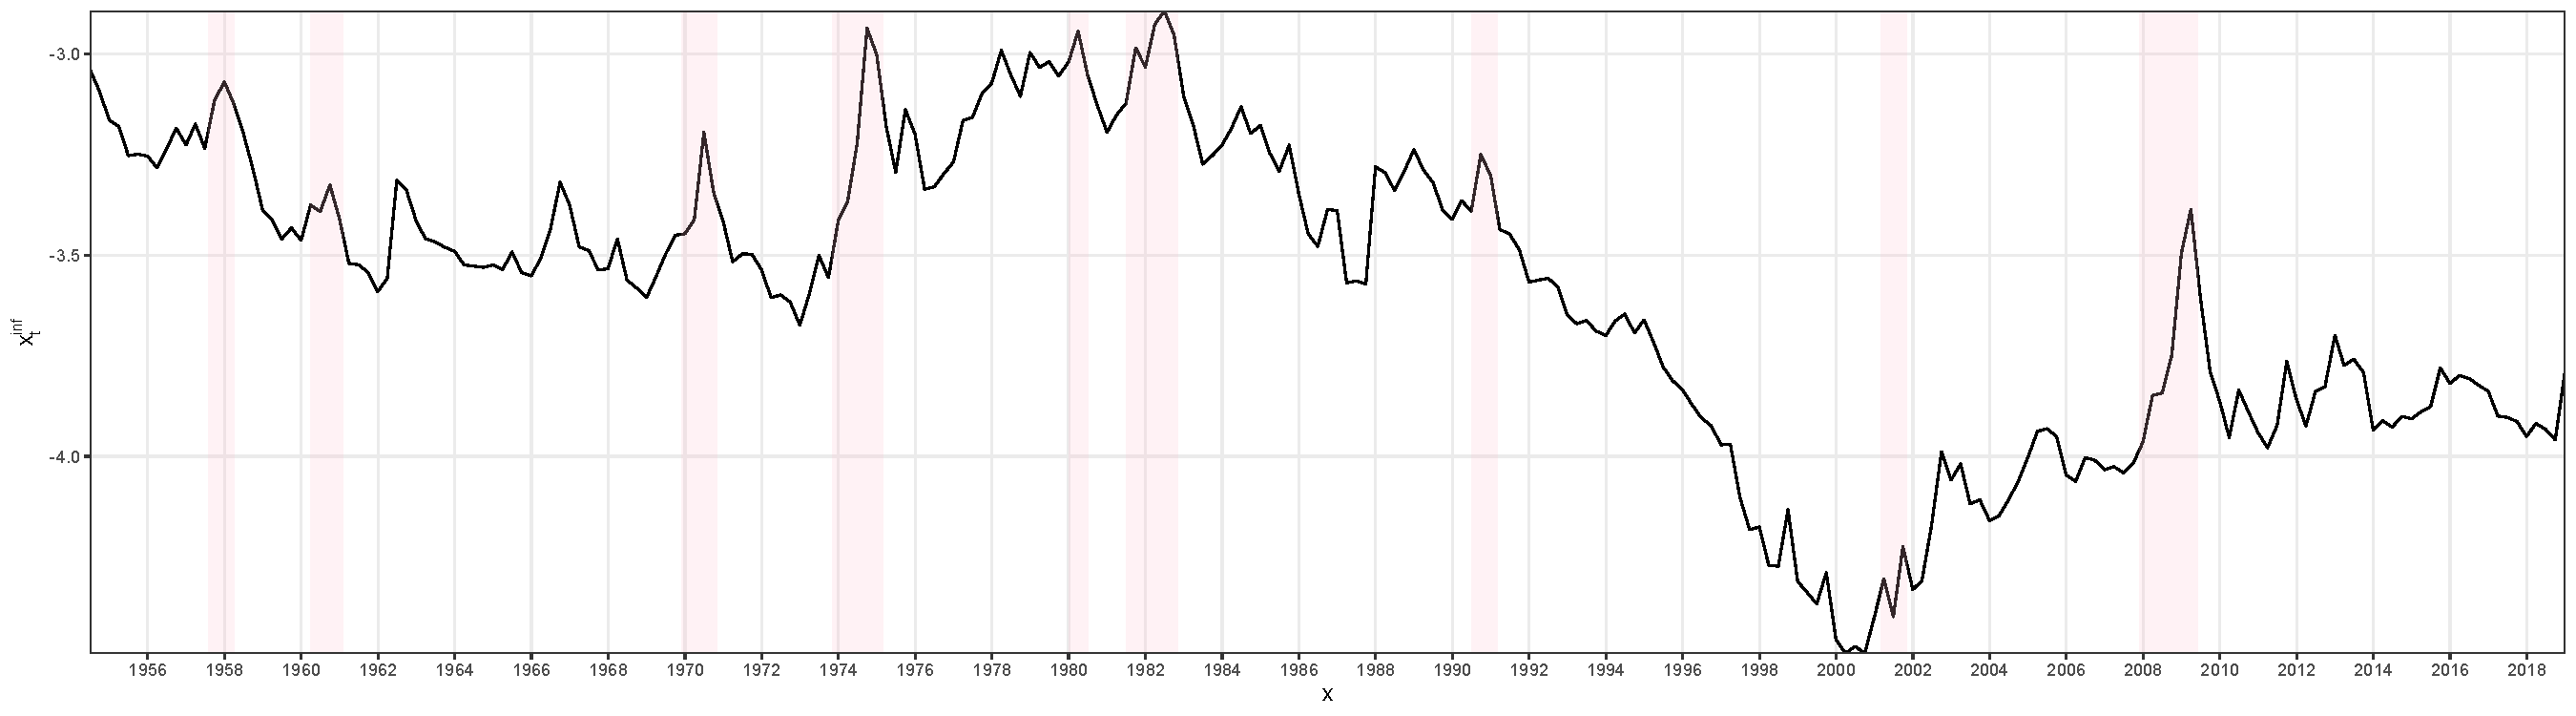
\includegraphics[width=1\linewidth]{Master_Thesis_Andreas_Kracht_Frandsen_files/figure-latex/DP-tids-1} 

}

\caption{Tidsserie af log Dividend Price Ratio.}\label{fig:DP-tids}
\end{figure}

\begin{figure}[htbp!]

{\centering 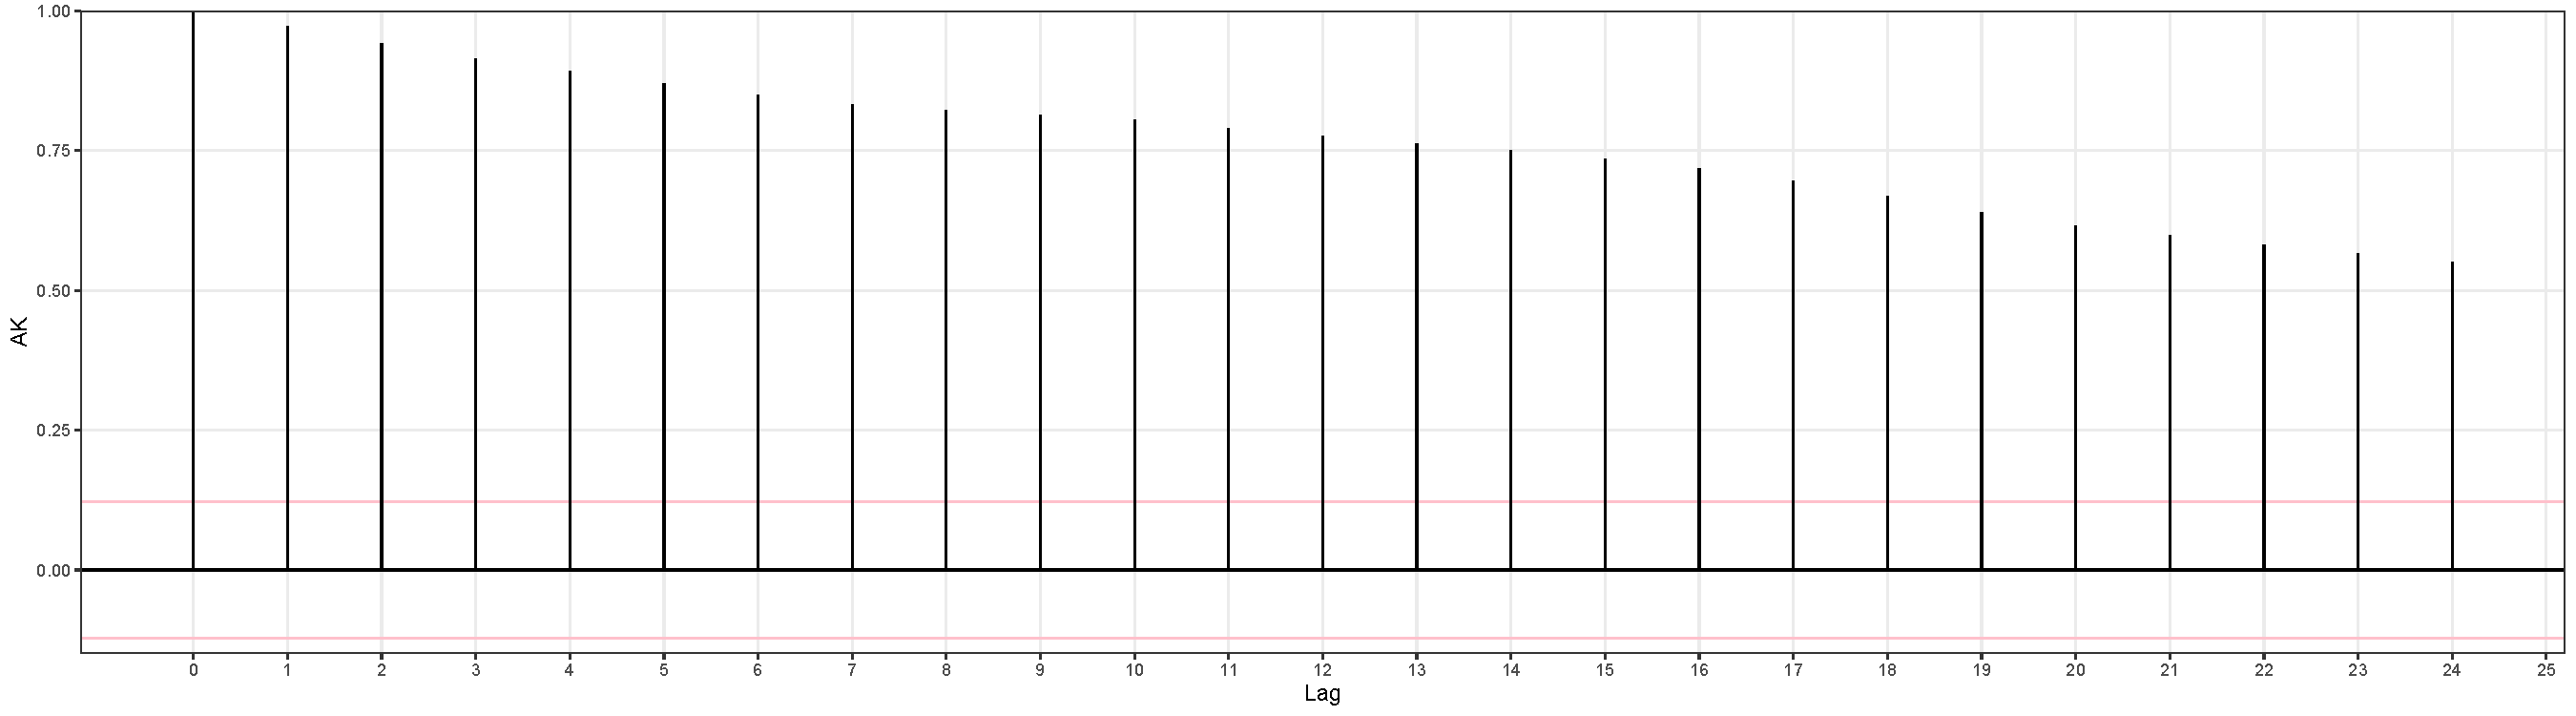
\includegraphics[width=1\linewidth]{Master_Thesis_Andreas_Kracht_Frandsen_files/figure-latex/DP-AK-1} 

}

\caption{Autokorrelation af log merafkastet af virksomhedsobligationer.}\label{fig:DP-AK}
\end{figure}

\begin{figure}[htbp!]

{\centering 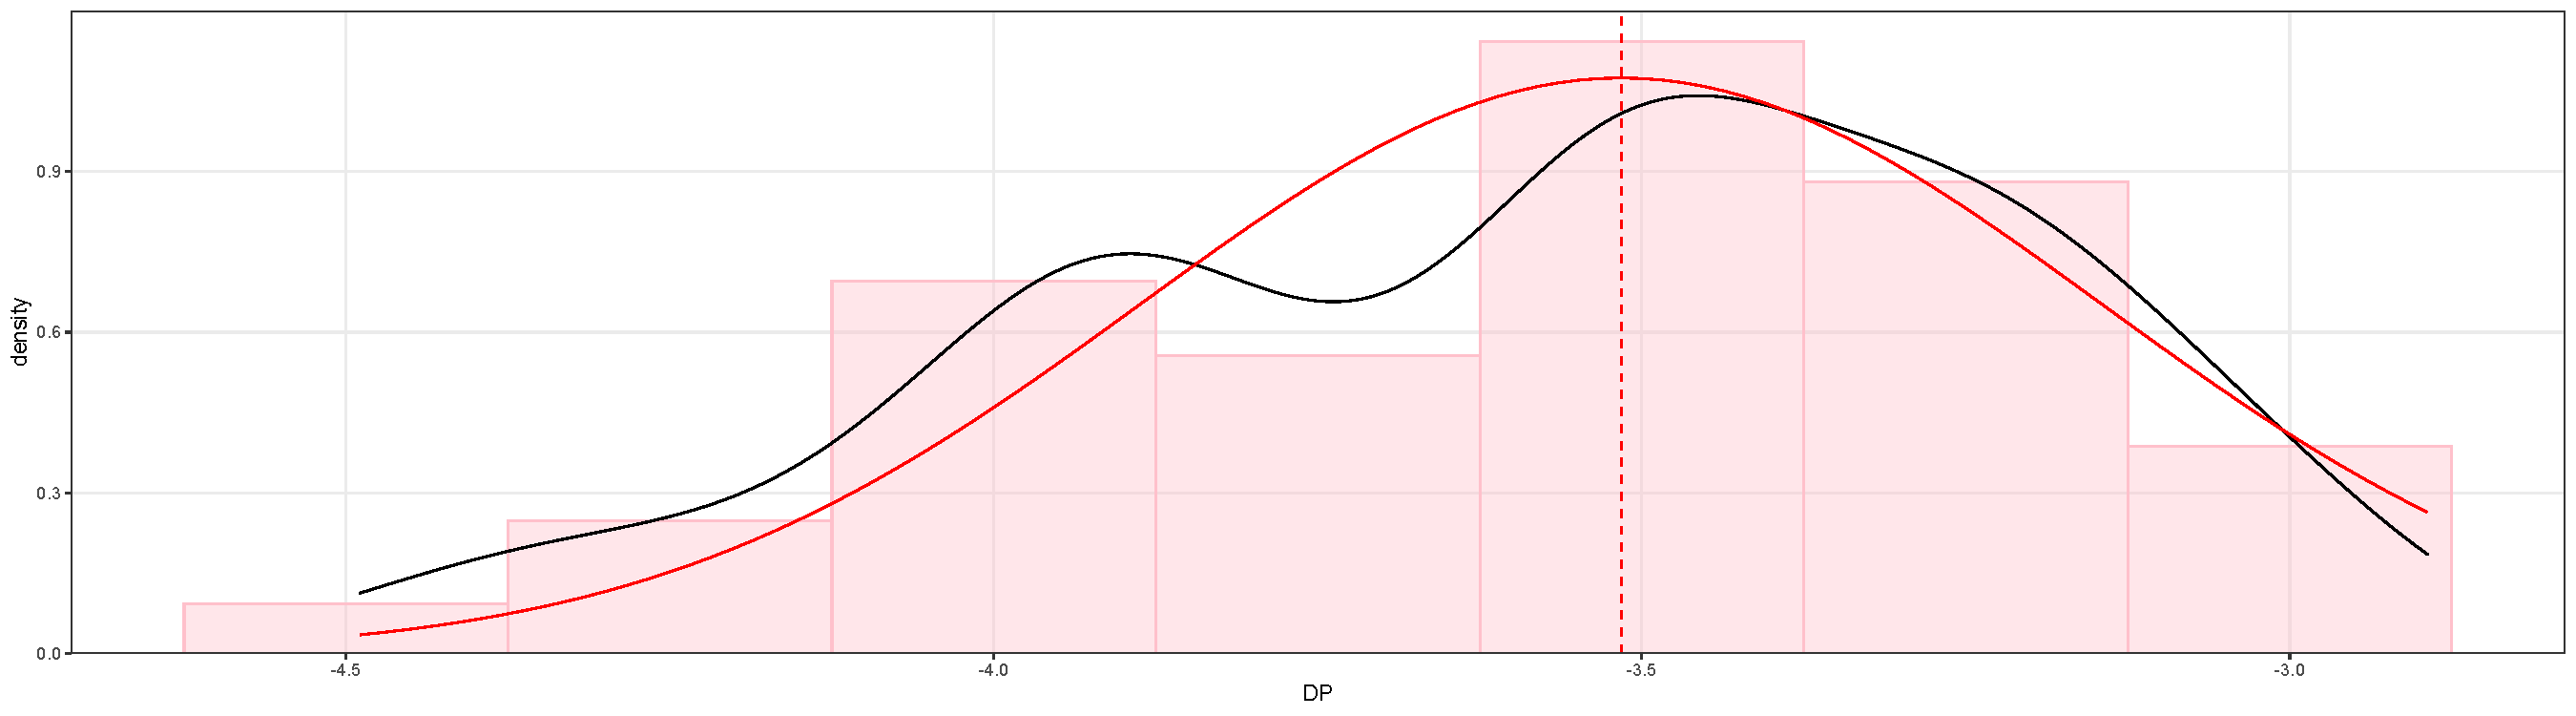
\includegraphics[width=1\linewidth]{Master_Thesis_Andreas_Kracht_Frandsen_files/figure-latex/DP-HIST-1} 

}

\caption{Autokorrelation af log netto renten.}\label{fig:DP-HIST}
\end{figure}

\hypertarget{price-earnings-ratio-x_ttextpe}{%
\subsection{\texorpdfstring{Price-Earnings Ratio -- \(x_t^{\text{pe}}\)}{Price-Earnings Ratio -- x\_t\^{}\{\textbackslash text\{pe\}\}}}\label{price-earnings-ratio-x_ttextpe}}

Priserne for forholdet mellem priser og indtjening er som ovenstående indeksniveauet fra Sektion \ref{dataak}, ekslusiv udbytte. Indtjeningen er en rullende sum repræsenterende indtjeningen på \emph{S\&P 500} indekset. Data er dermed fra hhv. \citep{CRSPakt}, hentet gennem \citep{WRDSakt} og \citep{Shiller2020}, hentet gennem \citep{Goyal2007}. At indtjeningen benytter et andet datagrundlag end aktieindekset kan skabe tvetydigheder i resultaterne, men prædiktabiltetsegenskaben for variablen er stadig intakt. Log \emph{Price Earnings Ratio} bliver da beregnet som forskellen mellem de kvartalsvise log priser og de kvartalvise log indtjeninger. Den justerede middelværdi er 2.754\(\%\). Standardafvigelsen er på 0.407\(\%\). Derudover haves en højreskæv leptokurtisk fordeling med hhv. skævhed på 0.958 og kurtosis på 7.52. Figur \ref{fig:PE-tids} viser et plot over tidsserien.

\begin{figure}[htbp!]

{\centering 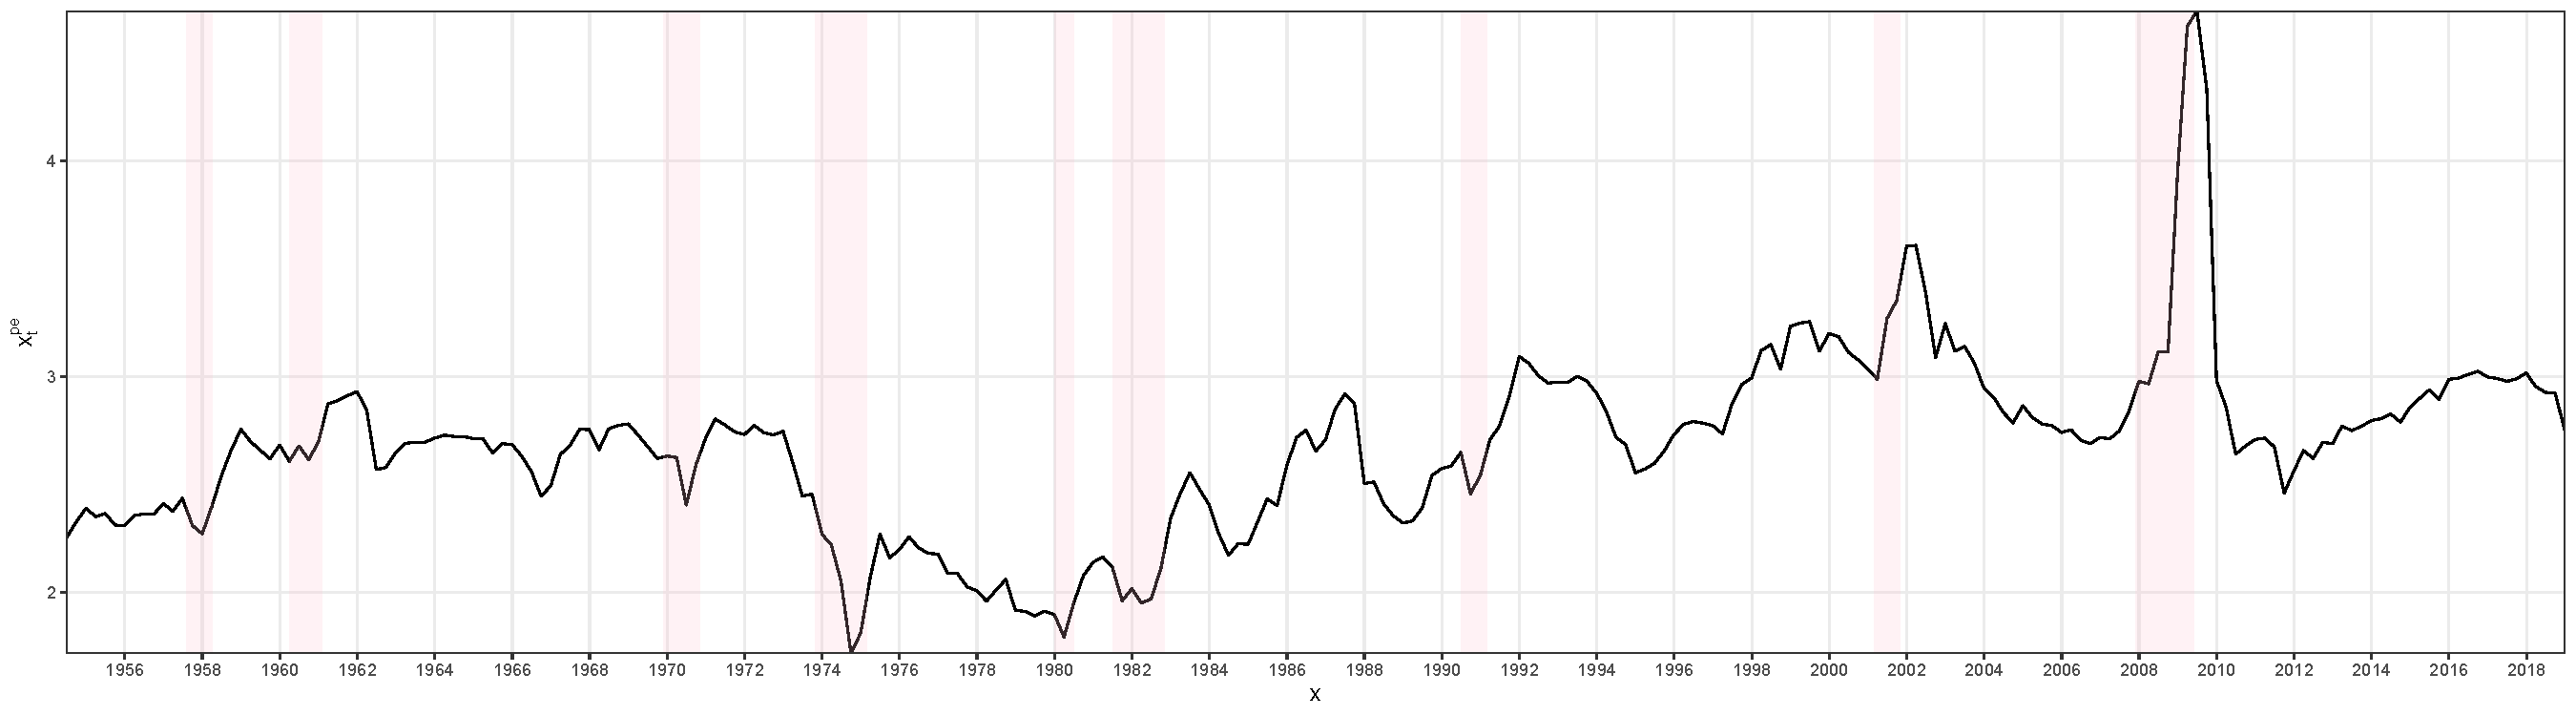
\includegraphics[width=1\linewidth]{Master_Thesis_Andreas_Kracht_Frandsen_files/figure-latex/PE-tids-1} 

}

\caption{Tidsserie af log Price Earnings Ratio.}\label{fig:PE-tids}
\end{figure}

\begin{figure}[htbp!]

{\centering 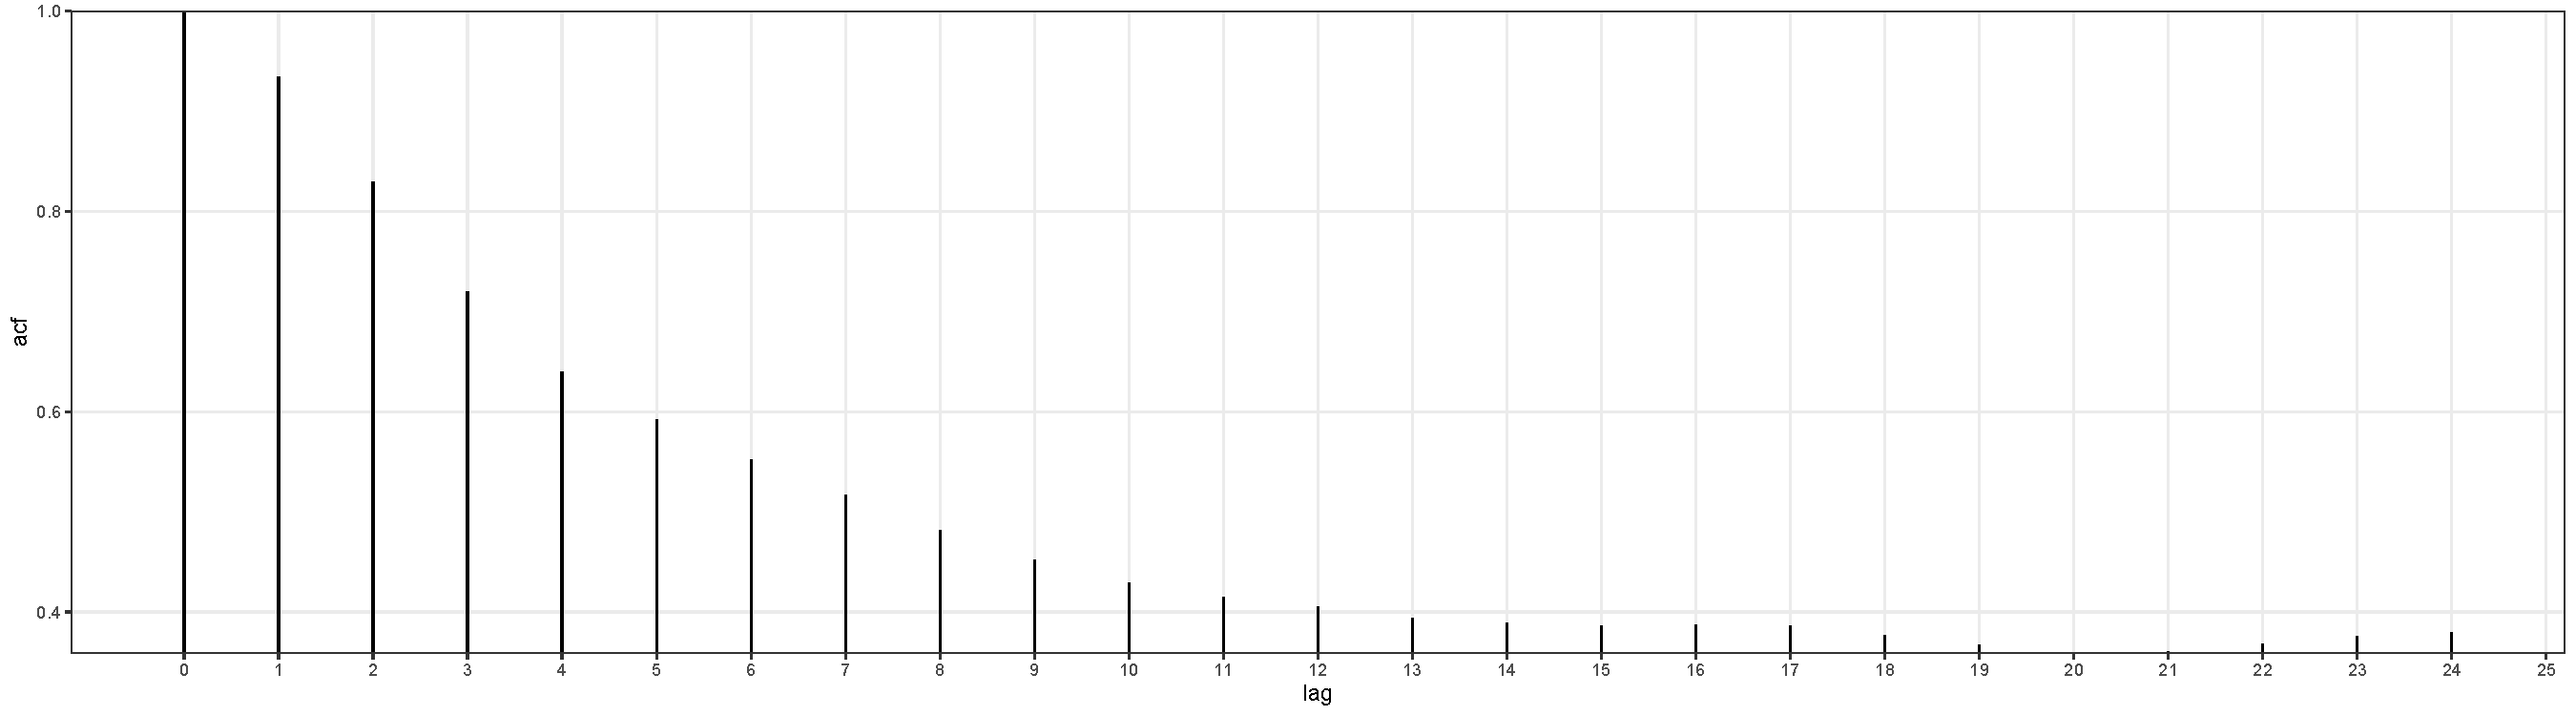
\includegraphics[width=1\linewidth]{Master_Thesis_Andreas_Kracht_Frandsen_files/figure-latex/PE-AK-1} 

}

\caption{Autokorrelation af log merafkastet af virksomhedsobligationer.}\label{fig:PE-AK}
\end{figure}

\begin{figure}[htbp!]

{\centering 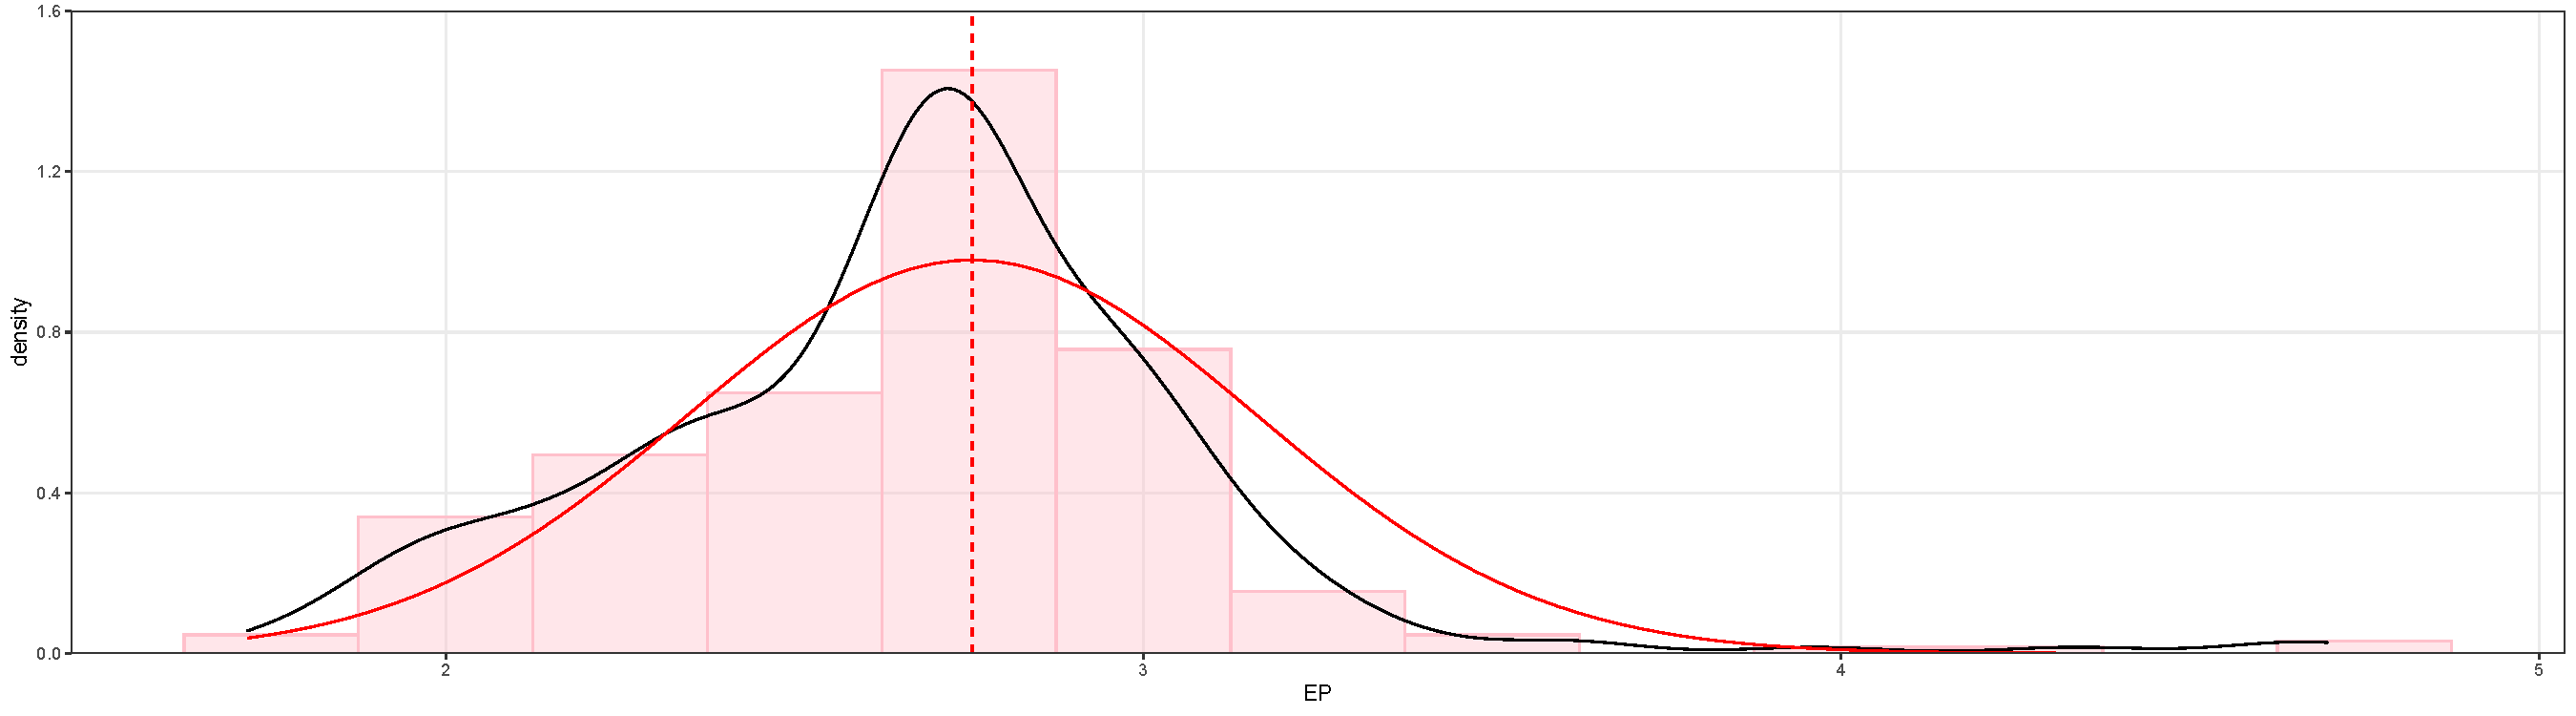
\includegraphics[width=1\linewidth]{Master_Thesis_Andreas_Kracht_Frandsen_files/figure-latex/PE-HIST-1} 

}

\caption{Autokorrelation af log netto renten.}\label{fig:PE-HIST}
\end{figure}

\hypertarget{book-to-market-ratio-x_ttextbm}{%
\subsection{\texorpdfstring{Book-to-Market Ratio -- \(x_t^{\text{bm}}\)}{Book-to-Market Ratio -- x\_t\^{}\{\textbackslash text\{bm\}\}}}\label{book-to-market-ratio-x_ttextbm}}

\emph{Book-to-market Ratio} er hentet gennem \citep{Goyal2007}. Bogførte værdier samt markedsværdier stammer fra \emph{Value Line}'s hjemmeside, mere specifikt gennem deres \emph{Long-Term Perspective Chart} af indekset \emph{Dow Jones Industrial Average}. Beregningsmetoden er oprindeligt månedsbaseret og for månederne marts til december beregnes forholdet som den bogførte værdi fra slutningen af sidste år, delt med prisen fra seneste månedsultimo. For januar og februar beregnes det som den bogførte værdi fra slutningen af for to år siden, delt med prisen fra seneste månedsultimo. Beregningsmetoden er sammenlignelig med \citep{Kothari1997} og \citep{Pontiff1998}. Det første og andet moment er hhv. 0.505 og 0.248. Fra tredje og fjerde moment ses højreskævhed og en mesokurtisk fordeling. \citep{Pontiff1998} finder første og andet moment til hhv. \(0.505\) og \(0.252\), hvilket validerer estimaterne. Efter 1982 ses det, at forholdet aftager kraftigt, og efter en kort tiltagning har det de seneste år stabiliseret sig. Dette kommer sig bl.a. af, at amerikanske virksomheder i stigende grad har bogført en negativ værdi, se evt. \emph{Historical Book Equity Data} fra \citep{French2020}. Figur \ref{fig:BM-tids} viser et plot over tidsserien.

\begin{figure}[htbp!]

{\centering 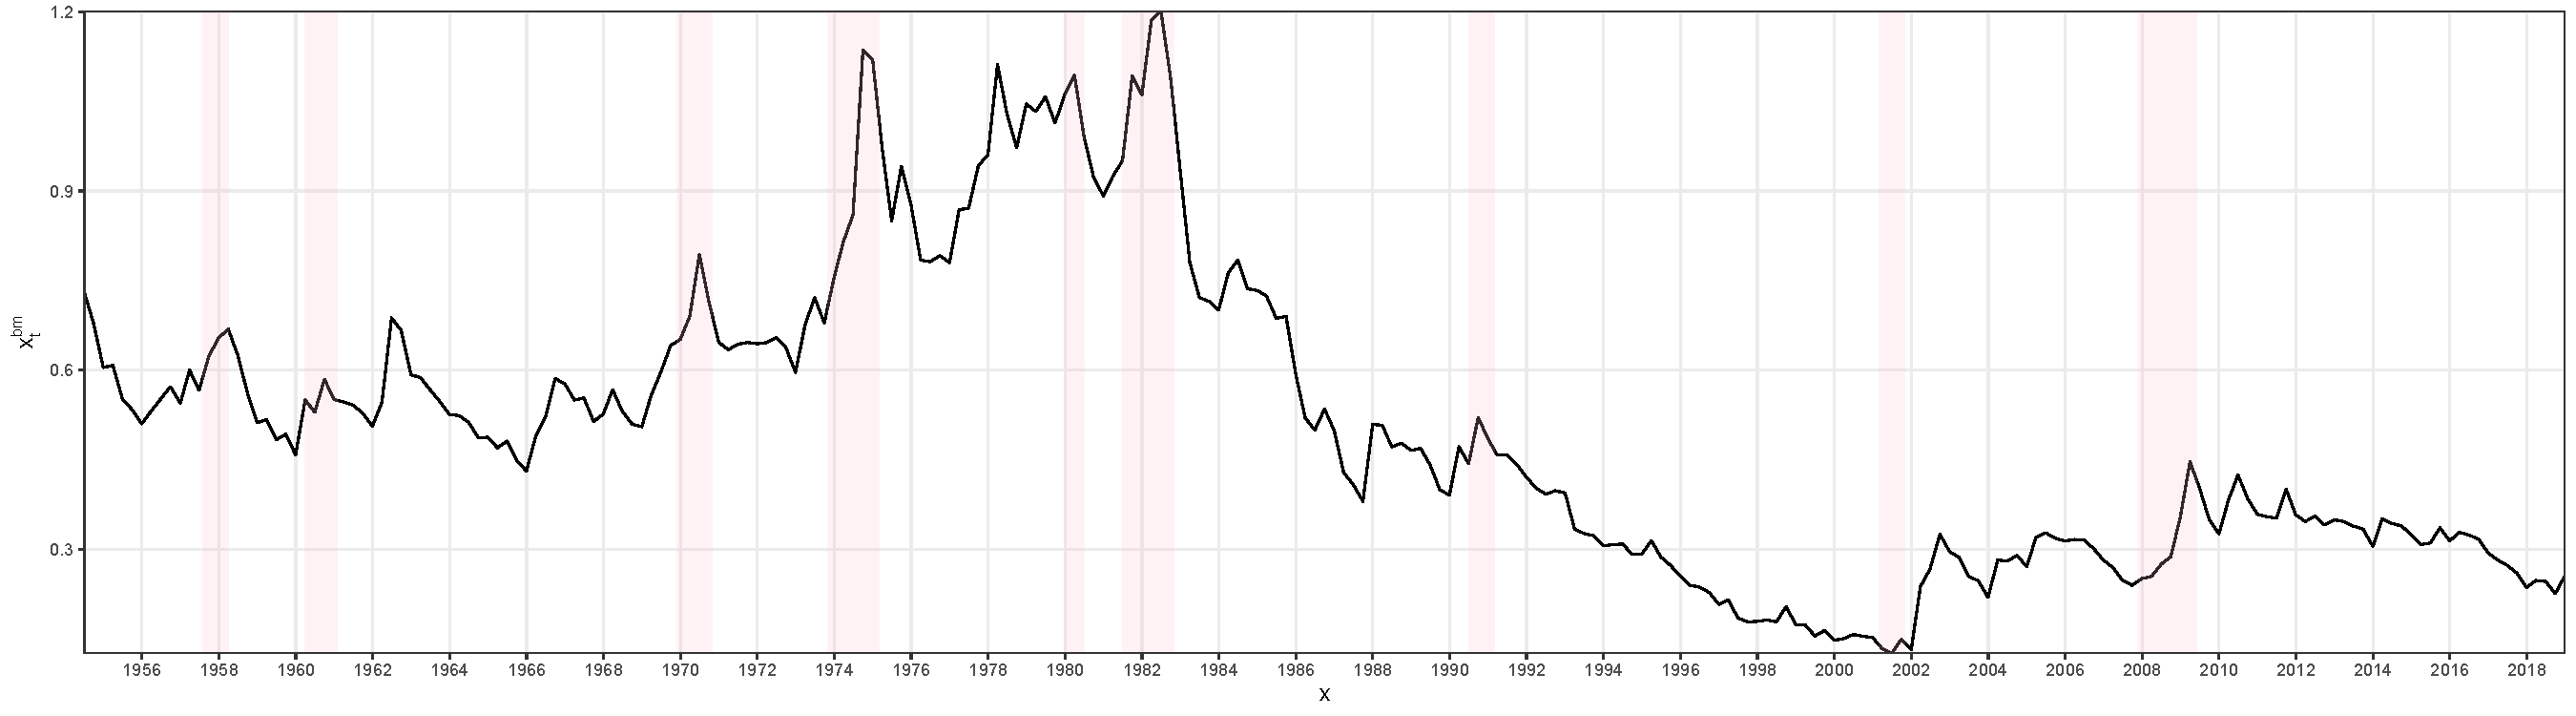
\includegraphics[width=1\linewidth]{Master_Thesis_Andreas_Kracht_Frandsen_files/figure-latex/BM-tids-1} 

}

\caption{Tidsserie af Book-to-market Ratio.}\label{fig:BM-tids}
\end{figure}

\begin{figure}[htbp!]

{\centering 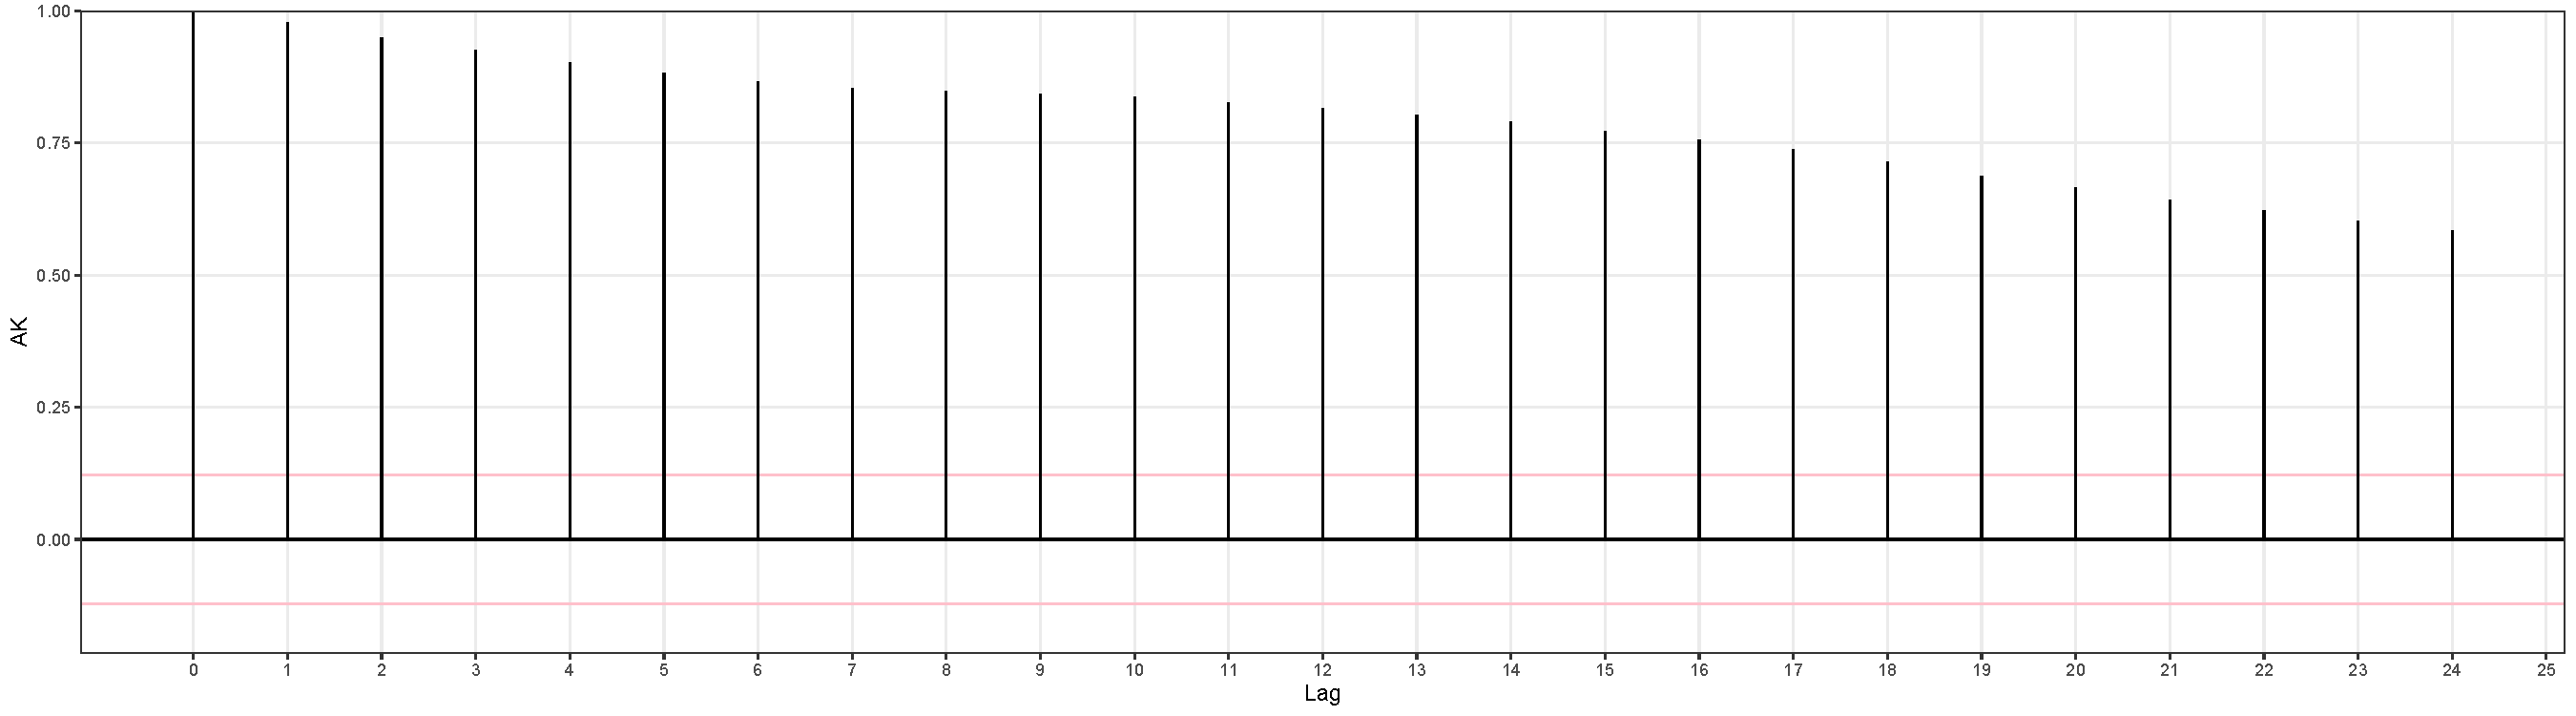
\includegraphics[width=1\linewidth]{Master_Thesis_Andreas_Kracht_Frandsen_files/figure-latex/BM-AK-1} 

}

\caption{Autokorrelation af log merafkastet af virksomhedsobligationer.}\label{fig:BM-AK}
\end{figure}

\begin{figure}[htbp!]

{\centering 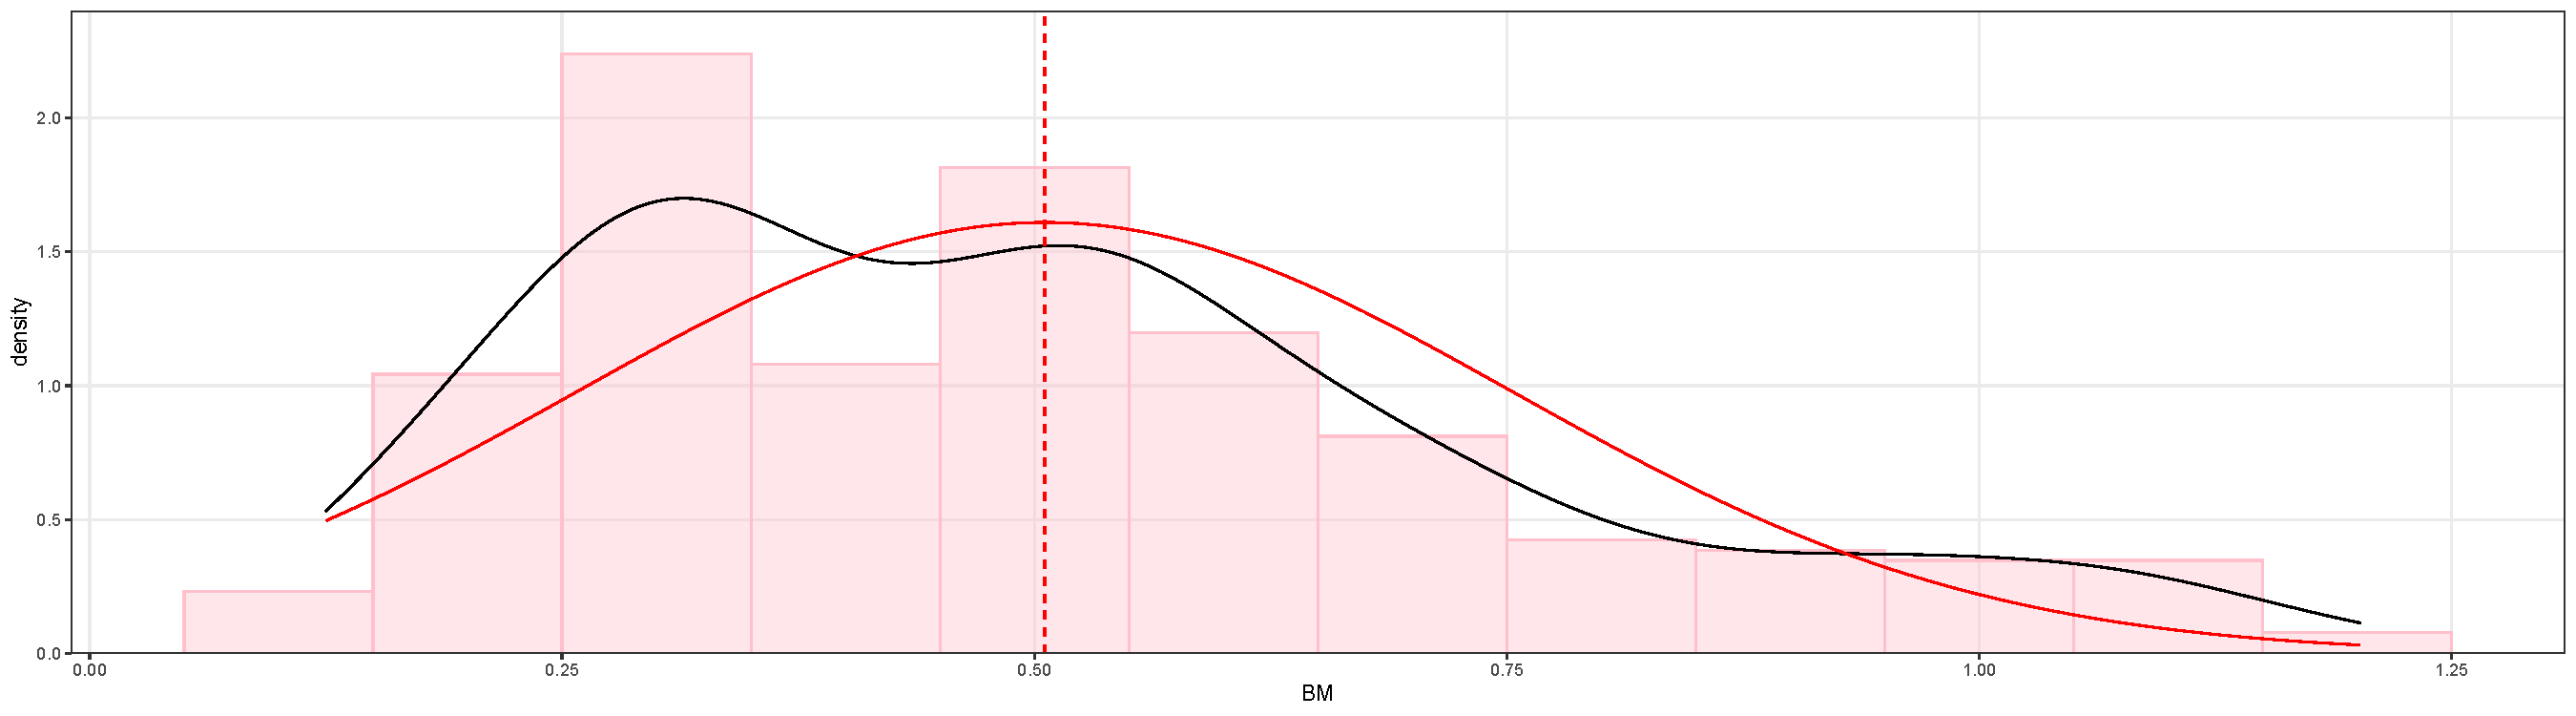
\includegraphics[width=1\linewidth]{Master_Thesis_Andreas_Kracht_Frandsen_files/figure-latex/BM-HIST-1} 

}

\caption{Autokorrelation af log netto renten.}\label{fig:BM-HIST}
\end{figure}

\hypertarget{aktievarians-x_ttextavar}{%
\subsection{\texorpdfstring{Aktievarians -- \(x_t^{\text{avar}}\)}{Aktievarians -- x\_t\^{}\{\textbackslash text\{avar\}\}}}\label{aktievarians-x_ttextavar}}

Aktievariansen består af den kvartalsvise kvadratsum af afkast, samt summen af produktet mellem to tilstødende kvartalsvise afkast. Beregningsmetoden er fra \citep{Schwert1987} og data er hentet gennem \citep{Goyal2007}, som baserer estimaterne på afkast fra \emph{S\&P 500} indekset. Selve metoden tager udgangspunkt i daglige priser fremfor kvartalsvise, for at måle det kvartalsvise aktieafkast \(r_{it}\). De kvartalsvise afkast er herefter kvadreret for at etablere variansen. Herefter justeres for autokorrelation, ved at addere to gange summen af produkterne mellem alle par af foreløbende kvartalsafkast. Middelværdien estimeres til 0.006 og med en standardafvigelse på 0.01. Givet ikke-negativiteten af variansen, ses forventeligt en meget højreskæv fordeling med tilhørende høj kurtosis på hhv. 7.186 og 68.38. Figur \ref{fig:AV-tids} viser et plot over tidsserien.

\begin{figure}[htbp!]

{\centering 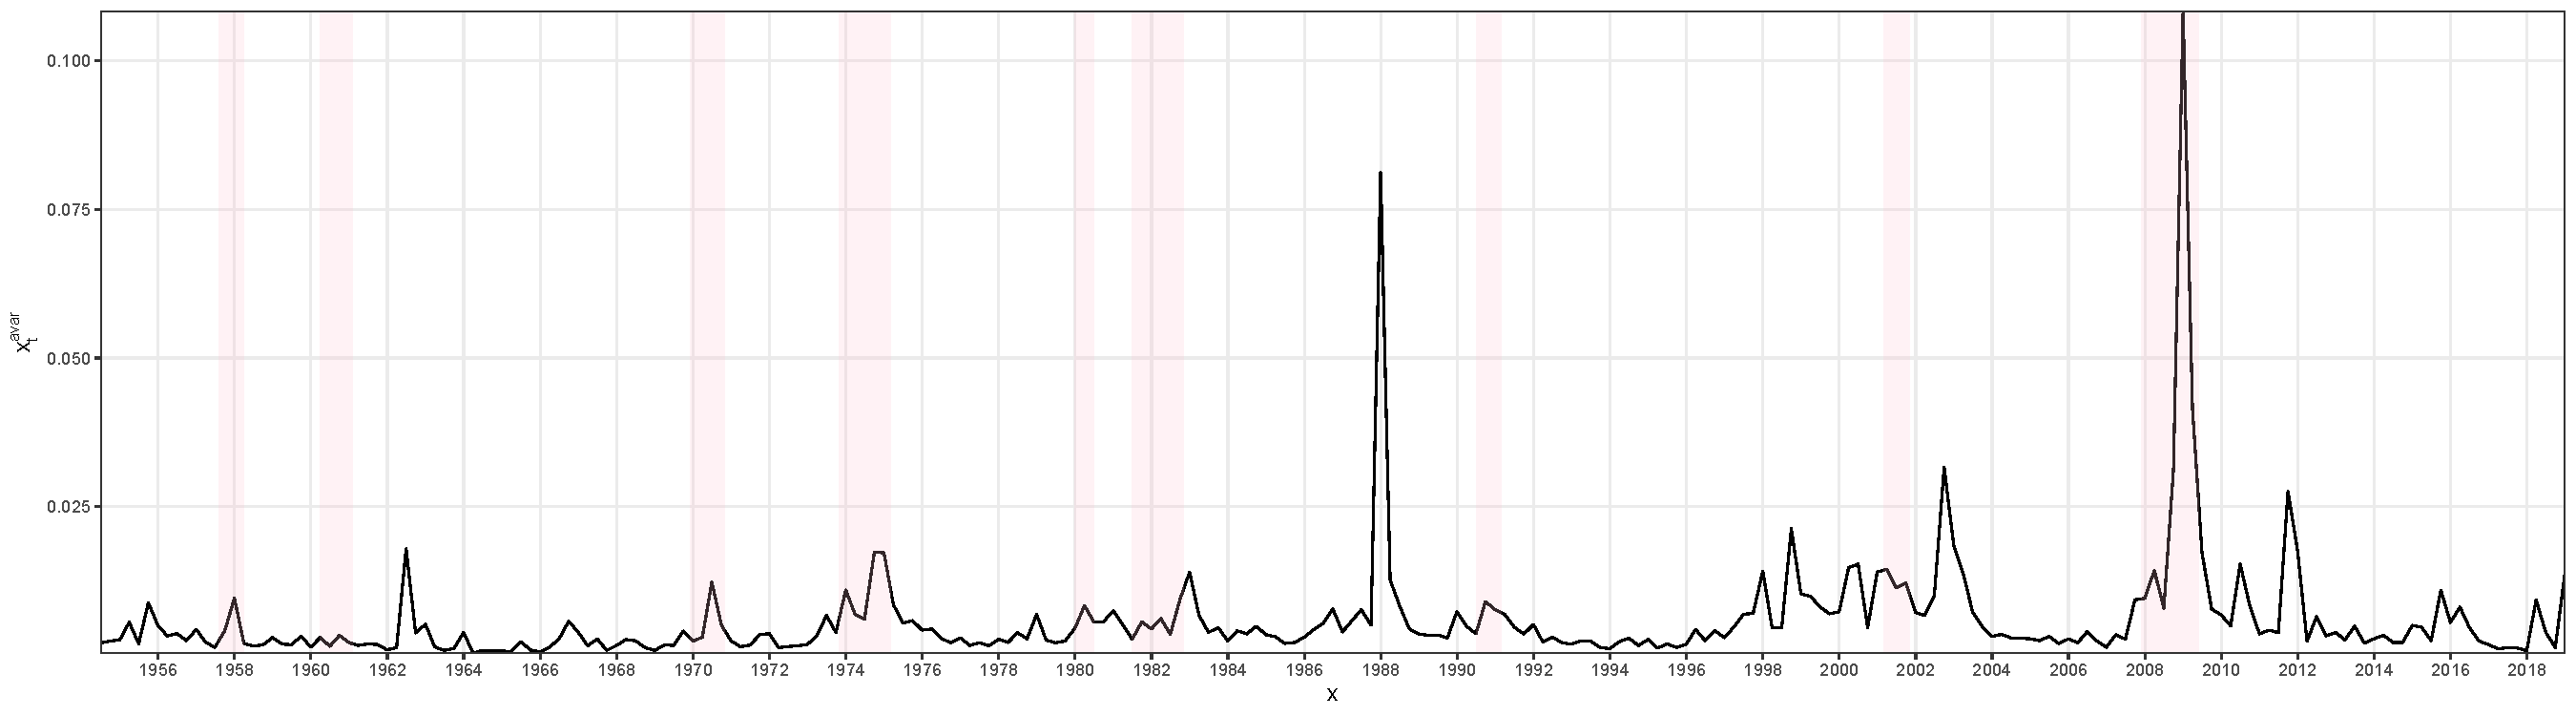
\includegraphics[width=1\linewidth]{Master_Thesis_Andreas_Kracht_Frandsen_files/figure-latex/AV-tids-1} 

}

\caption{Tidsserie af aktievariansen.}\label{fig:AV-tids}
\end{figure}

\begin{figure}[htbp!]

{\centering 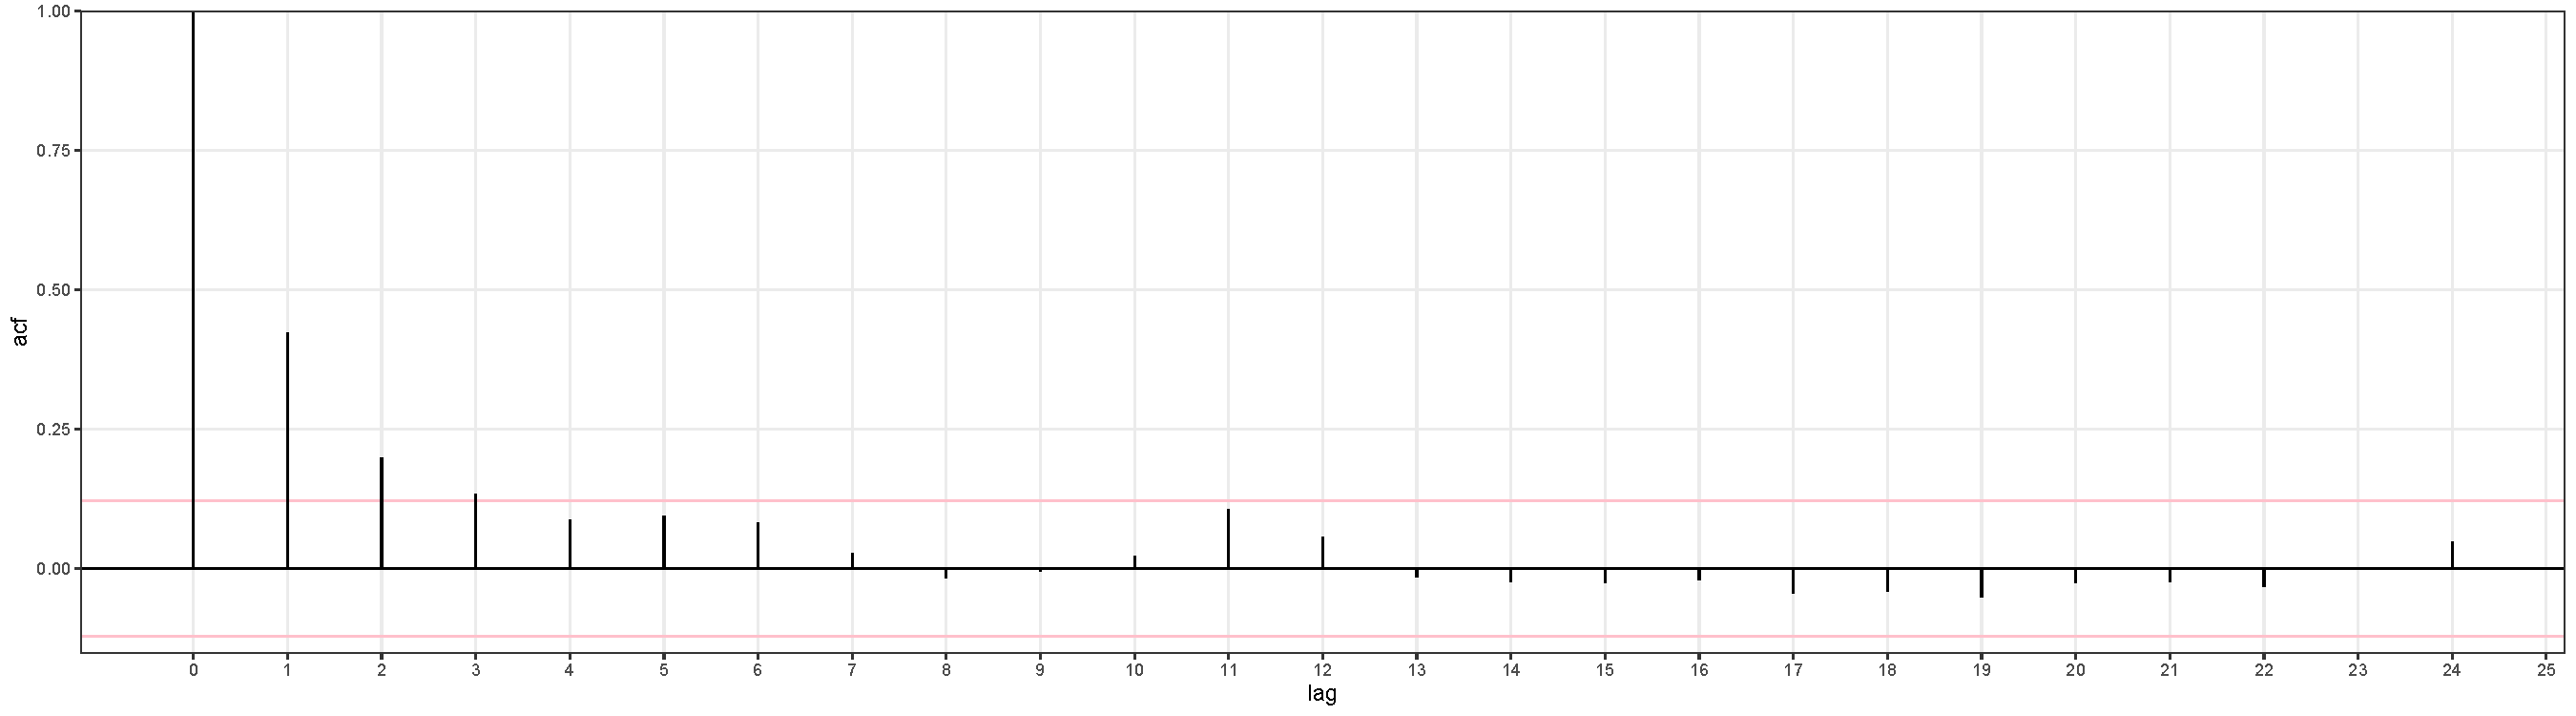
\includegraphics[width=1\linewidth]{Master_Thesis_Andreas_Kracht_Frandsen_files/figure-latex/AV-AK-1} 

}

\caption{Autokorrelation af log merafkastet af virksomhedsobligationer.}\label{fig:AV-AK}
\end{figure}

\begin{figure}[htbp!]

{\centering 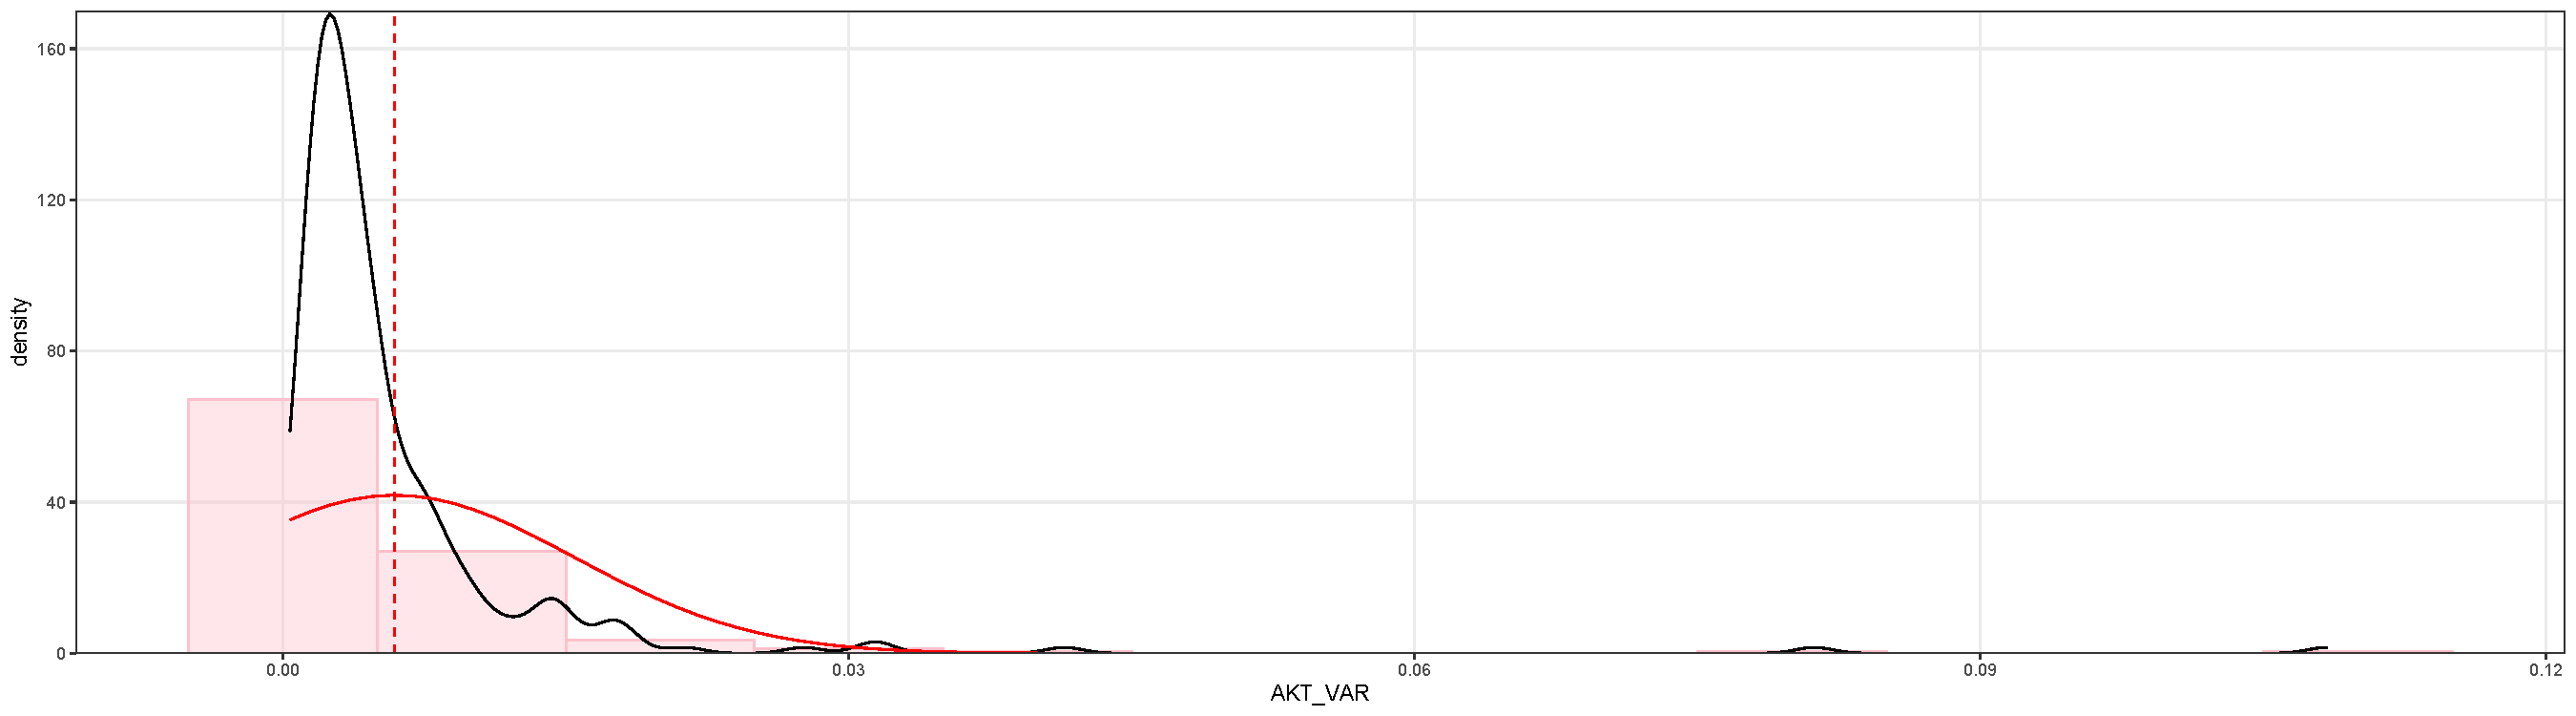
\includegraphics[width=1\linewidth]{Master_Thesis_Andreas_Kracht_Frandsen_files/figure-latex/AV-HIST-1} 

}

\caption{Autokorrelation af log netto renten.}\label{fig:AV-HIST}
\end{figure}

\hypertarget{datahml}{%
\subsection{\texorpdfstring{High Minus Low -- \(x_t^{\text{hml}}\)}{High Minus Low -- x\_t\^{}\{\textbackslash text\{hml\}\}}}\label{datahml}}

Den første af de to \emph{Fama-French} faktorer. Månedlige værdier er fra \citep{CRSPakt} og hentet gennem \citep{French2020}, det er herefter omdannet til kvartalsvise værdier via et kvartalsvist rullende tre-måneders gennemsnit. Selve faktoren er baseret på: to porteføljer baseret på størrelse, hvor skillelinjen er markedsmedianen på \emph{NYSE}, tre porteføljer baseret på \emph{Book-to-Market Ratio}, hvor skilningerne er \(30\)- og \(70\)-percentilerne af \emph{Book-to-Market Ratio} på \emph{NYSE}. Herefter eksisterer der seks fællesmængder, som dermed udgør grundlaget for porteføljerne til \emph{High Minus Low}. Selve faktoren beregnes som gennemsnittet på de to værdi-porteføljer\footnote{Virksomheder i værdi-porteføljerne har høj \emph{Book-to-market Ratio} og er hhv. store og små.} fratrukket det gennemsnitlige afkast på de to vækst-porteføljer\footnote{Virksomheder i vækst-porteføljerne har lav \emph{Book-to-market Ratio} og er hhv. store og små.}. En positiv \emph{High Minus Low} faktor medfører, at værdi-virksomheder er mere efficiente end vækst virksomheder på lang sigt, \citep{French1993}. Det første og andet moment er hhv. 0.33 og 1.809. Skævhed på 0.447 og kurtosis på 4.858, indikerer en forholdsvis symmetrisk fordeling. Figur \ref{fig:HML-tids} viser et plot over tidsserien.

\begin{figure}[htbp!]

{\centering 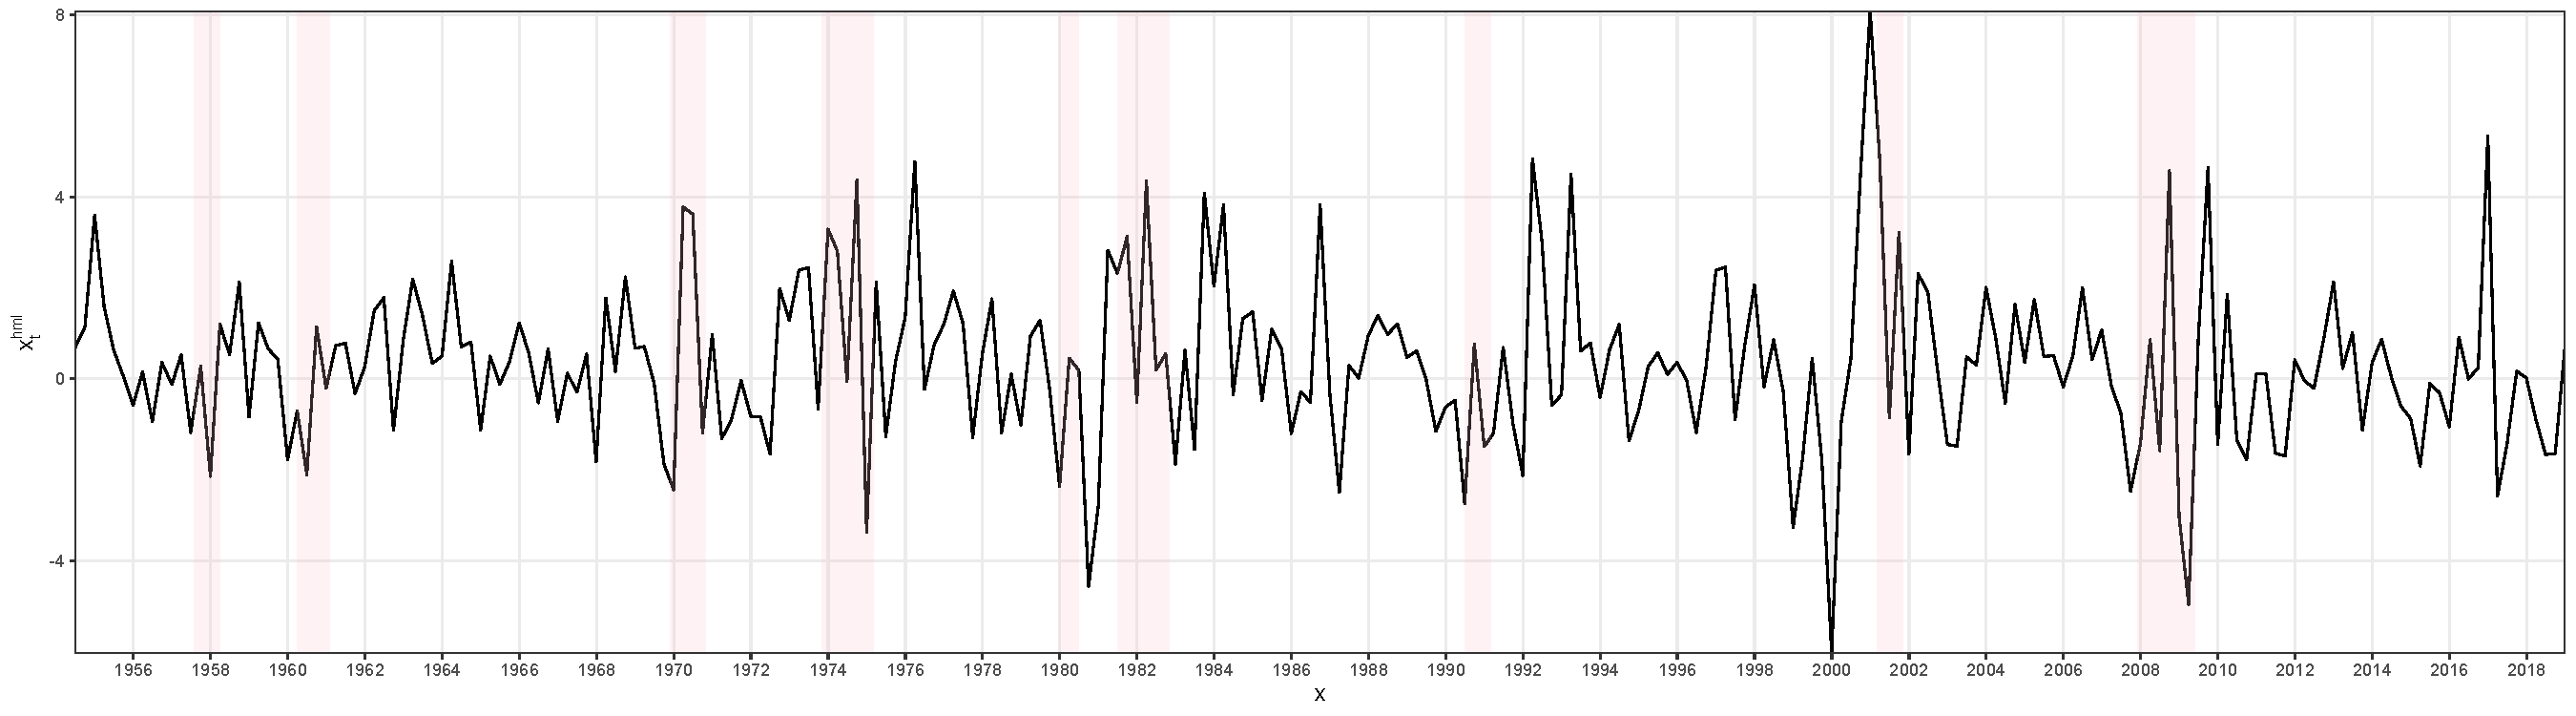
\includegraphics[width=1\linewidth]{Master_Thesis_Andreas_Kracht_Frandsen_files/figure-latex/HML-tids-1} 

}

\caption{Tidsserie af High Minus Low.}\label{fig:HML-tids}
\end{figure}

\begin{figure}[htbp!]

{\centering 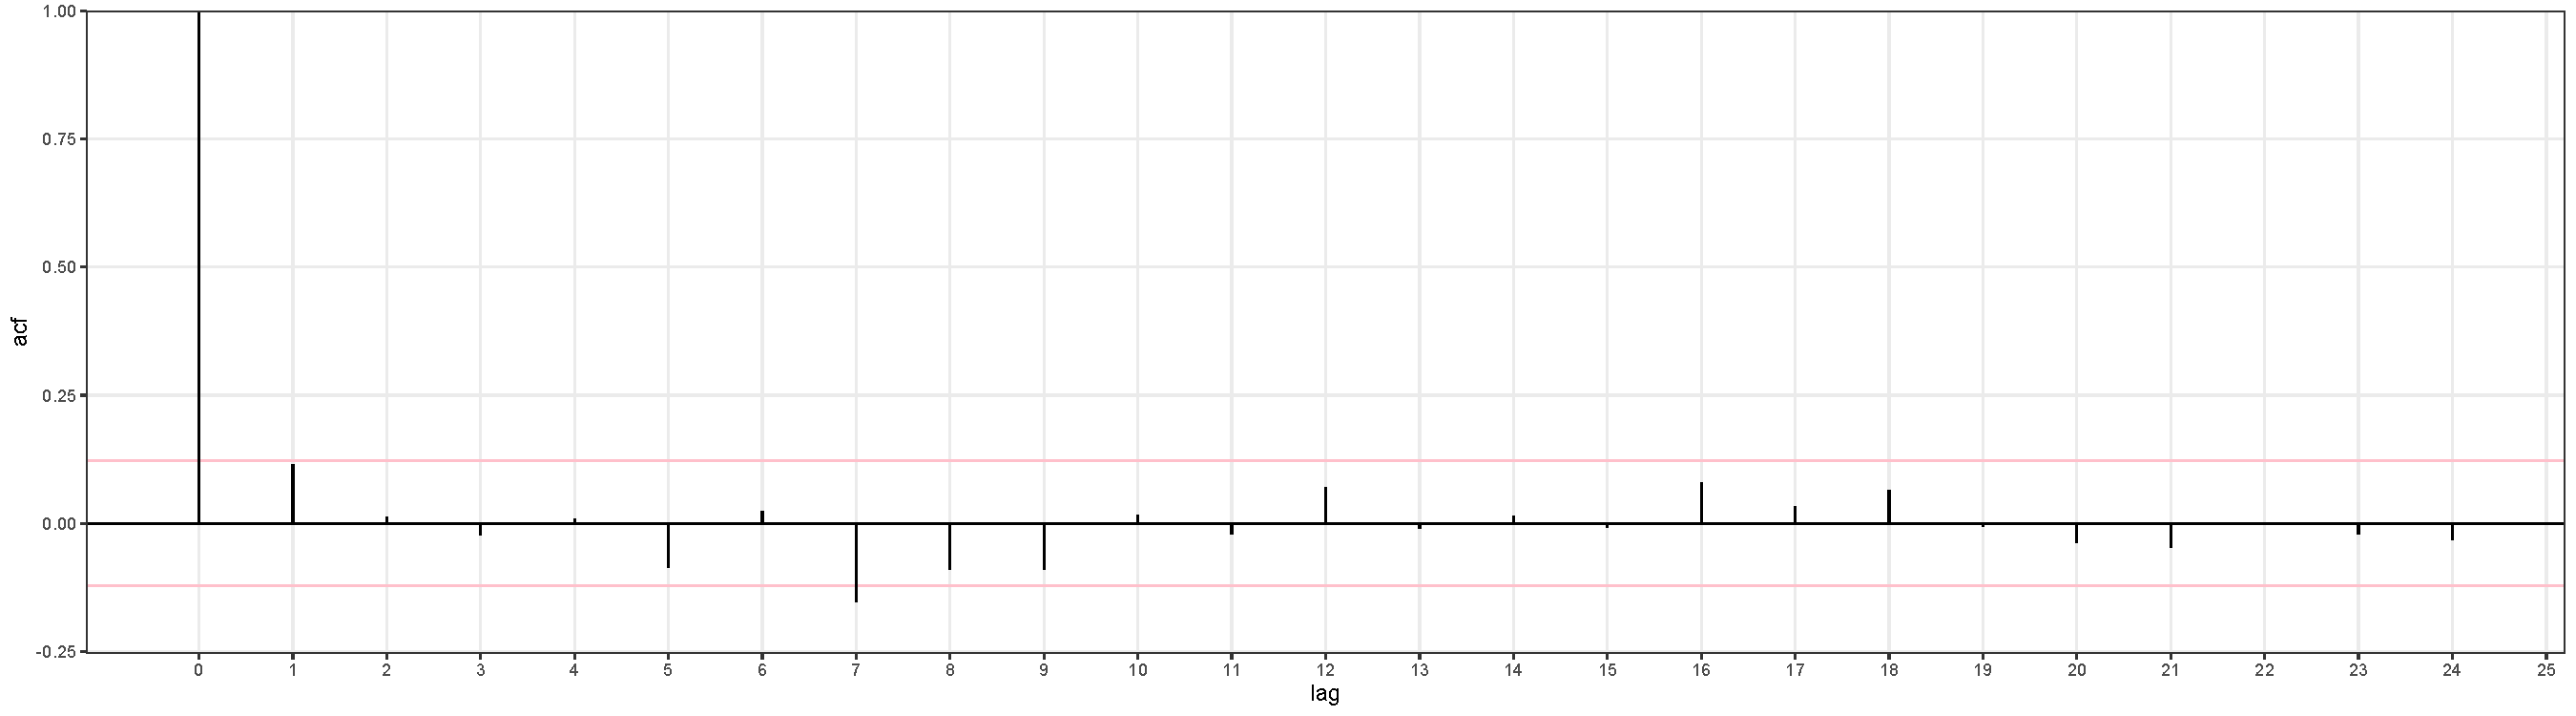
\includegraphics[width=1\linewidth]{Master_Thesis_Andreas_Kracht_Frandsen_files/figure-latex/HML-AK-1} 

}

\caption{Autokorrelation af log merafkastet af virksomhedsobligationer.}\label{fig:HML-AK}
\end{figure}

\begin{figure}[htbp!]

{\centering 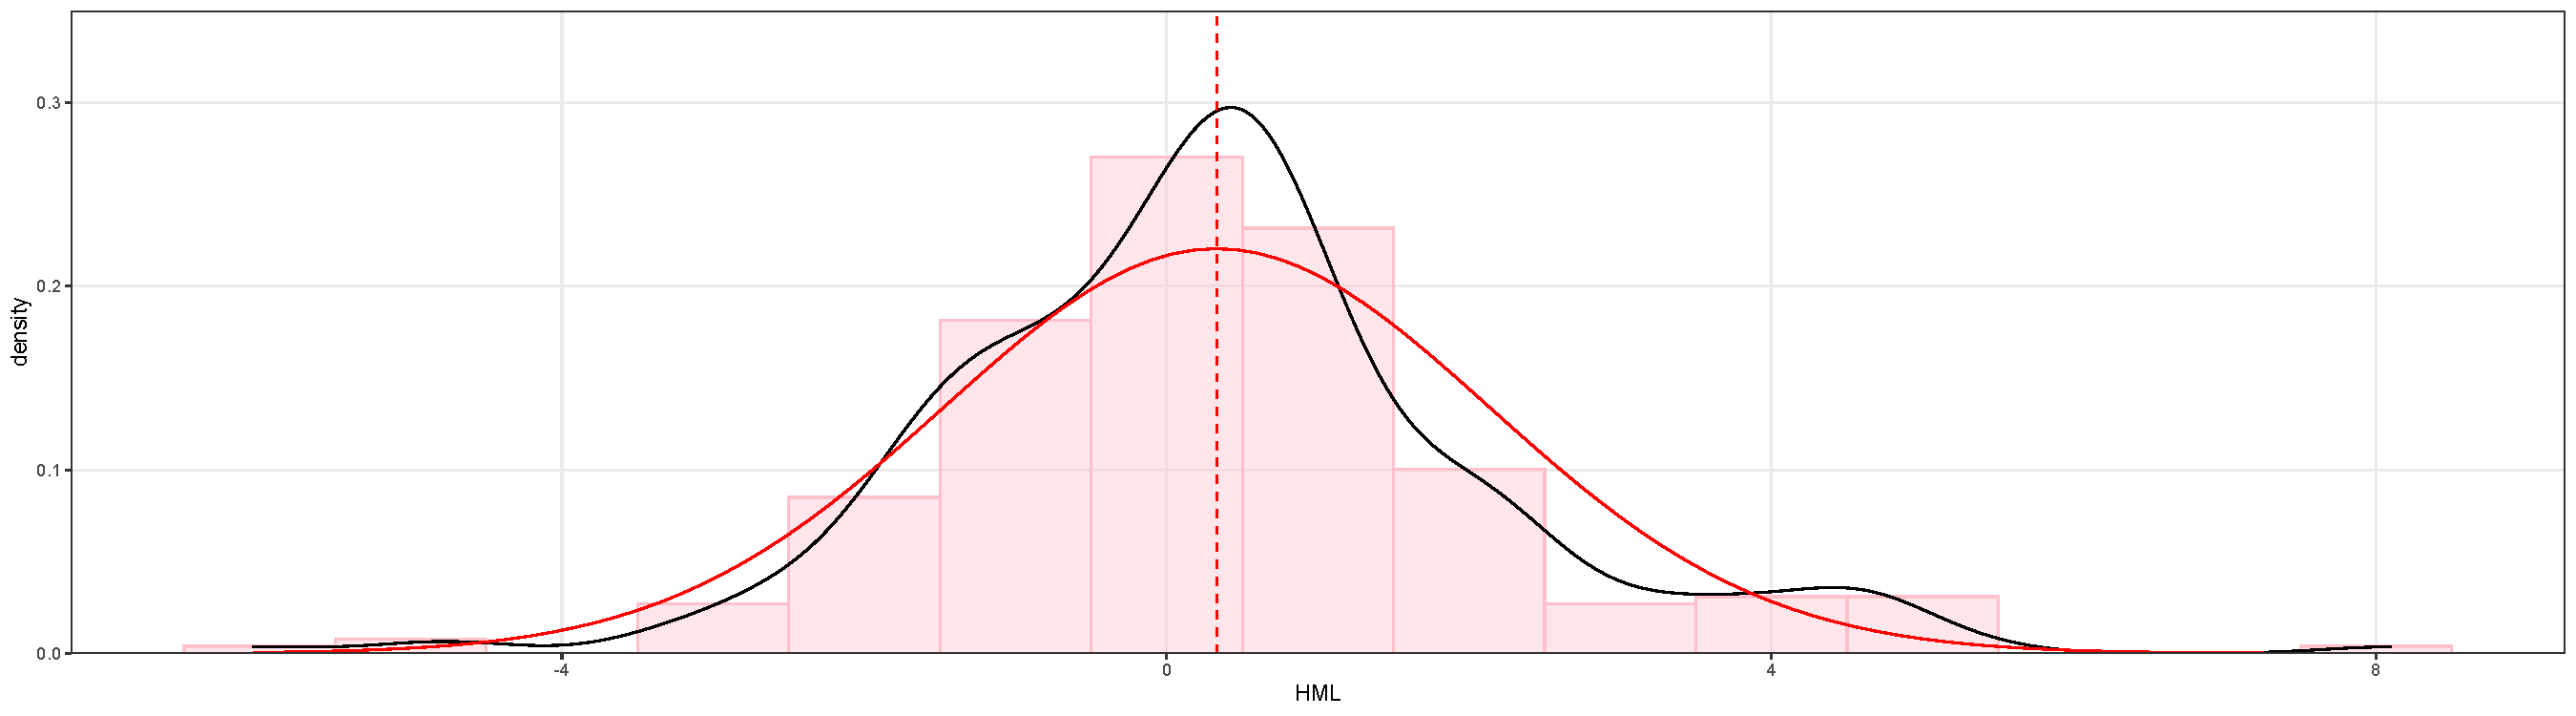
\includegraphics[width=1\linewidth]{Master_Thesis_Andreas_Kracht_Frandsen_files/figure-latex/HML-HIST-1} 

}

\caption{Autokorrelation af log netto renten.}\label{fig:HML-HIST}
\end{figure}

\hypertarget{datasmb}{%
\subsection{\texorpdfstring{Small Minus Big -- \(x_t^{\text{smb}}\)}{Small Minus Big -- x\_t\^{}\{\textbackslash text\{smb\}\}}}\label{datasmb}}

Den anden \emph{Fama-French} faktor. Månedlige værdier er fra \citep{CRSPakt} og hentet gennem \citep{French2020}, det er herefter omdannet til kvartalsvise værdier via et kvartalsvist rullende tre-måneders gennemsnit. Selve faktoren er baseret på de samme porteføljer som beskrevet i ovenstående Sektion \ref{datahml}. Selve faktoren beregnes som forskellen mellem de ligevægtede gennemsnitlige afkast af de små porteføljer og de store porteføljer. En positiv \emph{Small Minus Big} faktor er også kendt som \emph{Small Firm Effect}, og medfører, at små virksomheder er mere efficiente end store virksomheder på lang sigt, \citep{French1993}. Det første og andet moment er hhv. 0.168 og 1.717. En skævhed på 0.125 og kurtosis på 3.025, indikerer en meget symmetrisk fordeling. Figur \ref{fig:SMB-tids} viser et plot over tidsserien.

\begin{figure}[htbp!]

{\centering 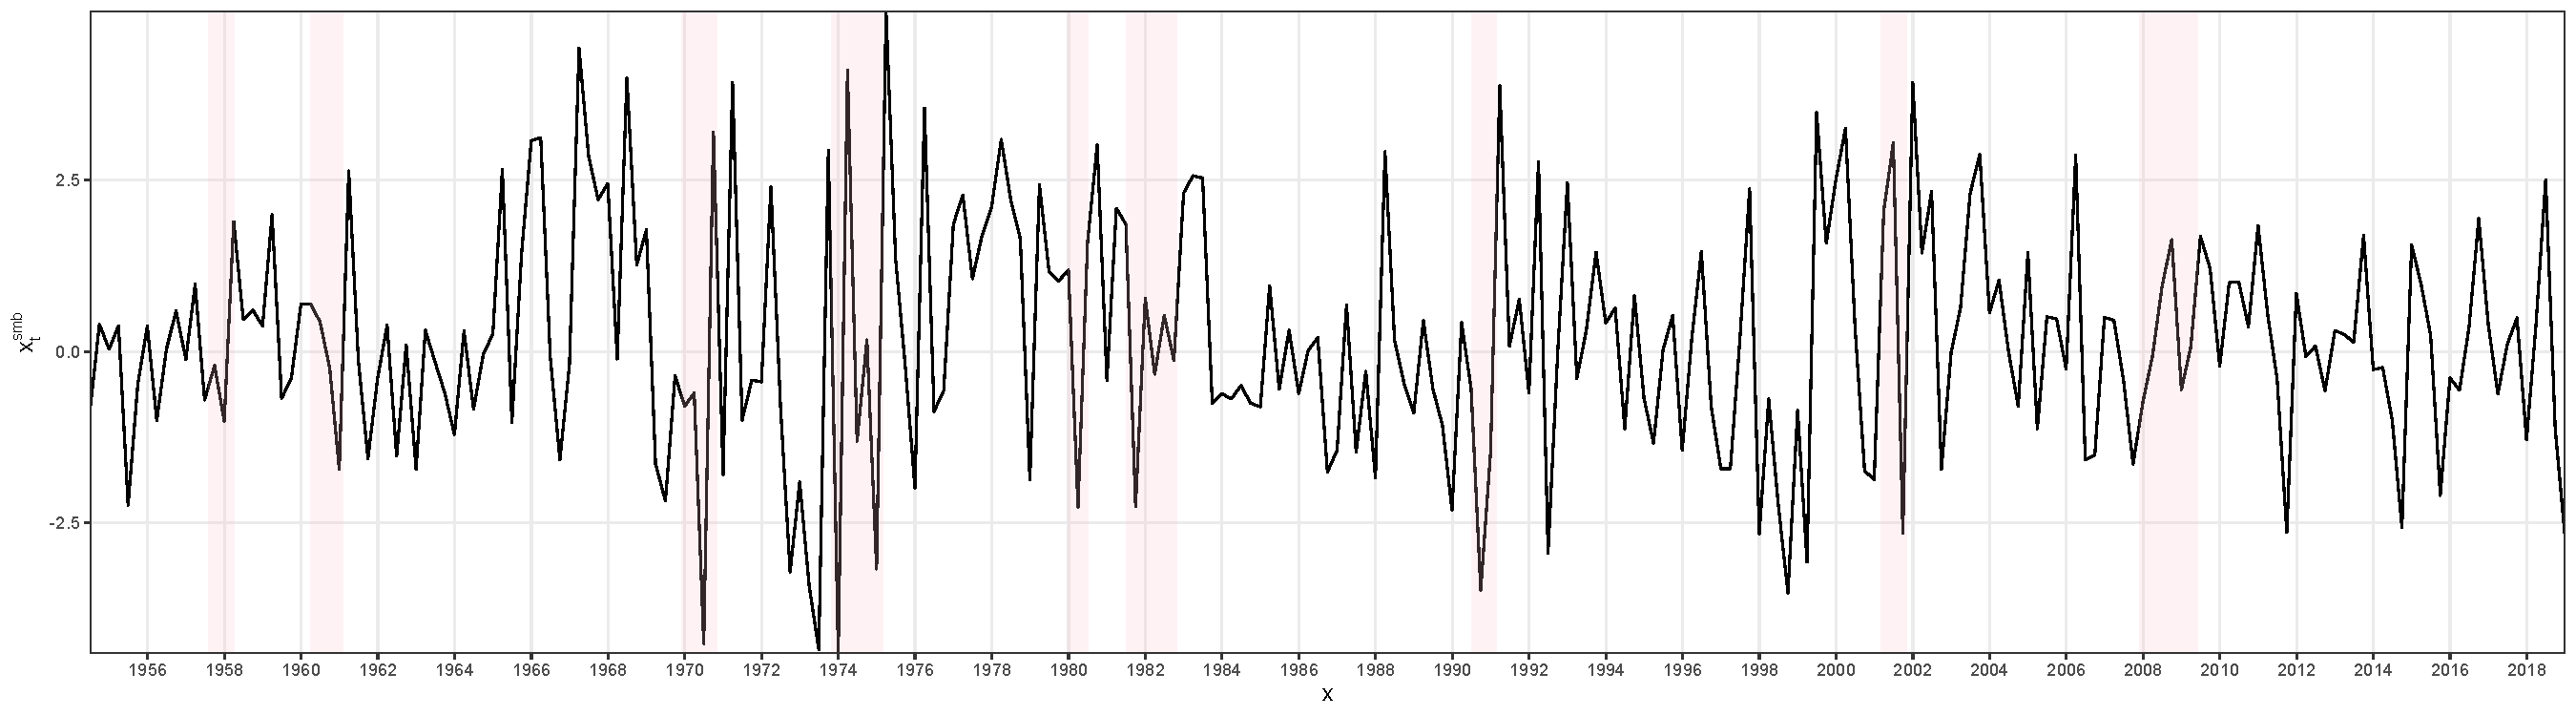
\includegraphics[width=1\linewidth]{Master_Thesis_Andreas_Kracht_Frandsen_files/figure-latex/SMB-tids-1} 

}

\caption{Tidsserie af Small Minus Big.}\label{fig:SMB-tids}
\end{figure}

\begin{figure}[htbp!]

{\centering 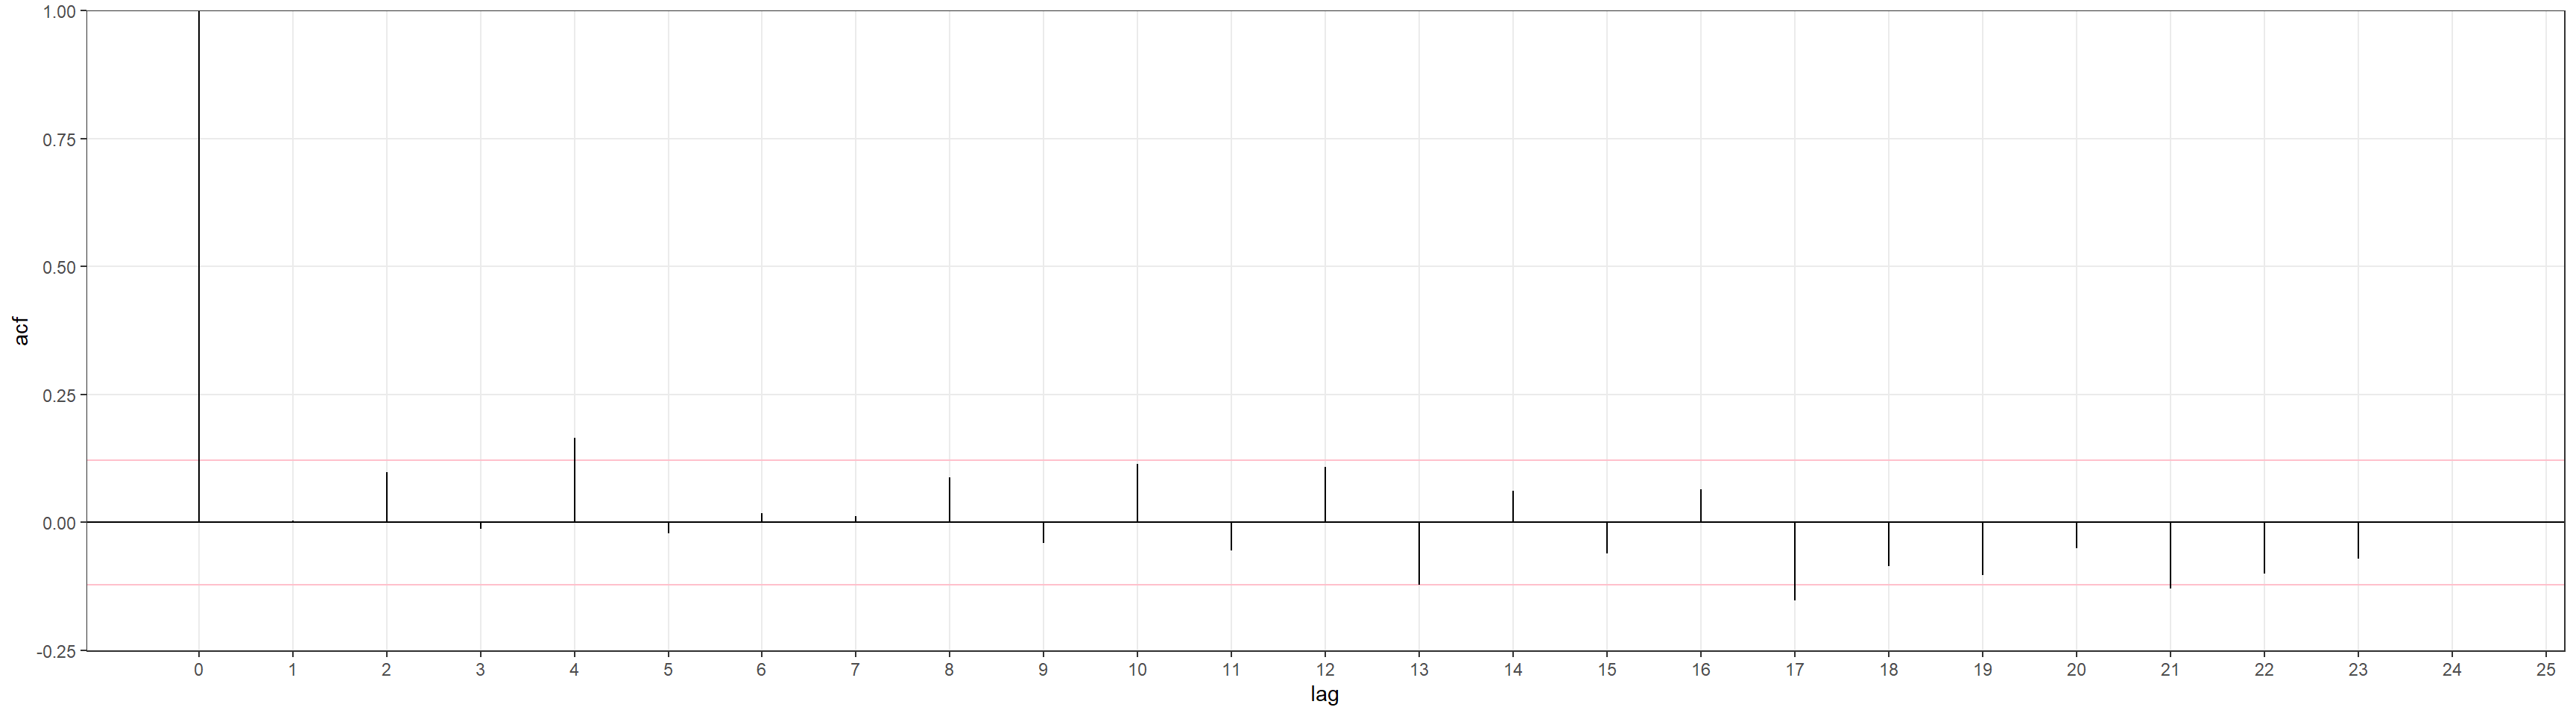
\includegraphics[width=1\linewidth]{Master_Thesis_Andreas_Kracht_Frandsen_files/figure-latex/SMB-AK-1} 

}

\caption{Autokorrelation af log merafkastet af virksomhedsobligationer.}\label{fig:SMB-AK}
\end{figure}

\begin{figure}[htbp!]

{\centering 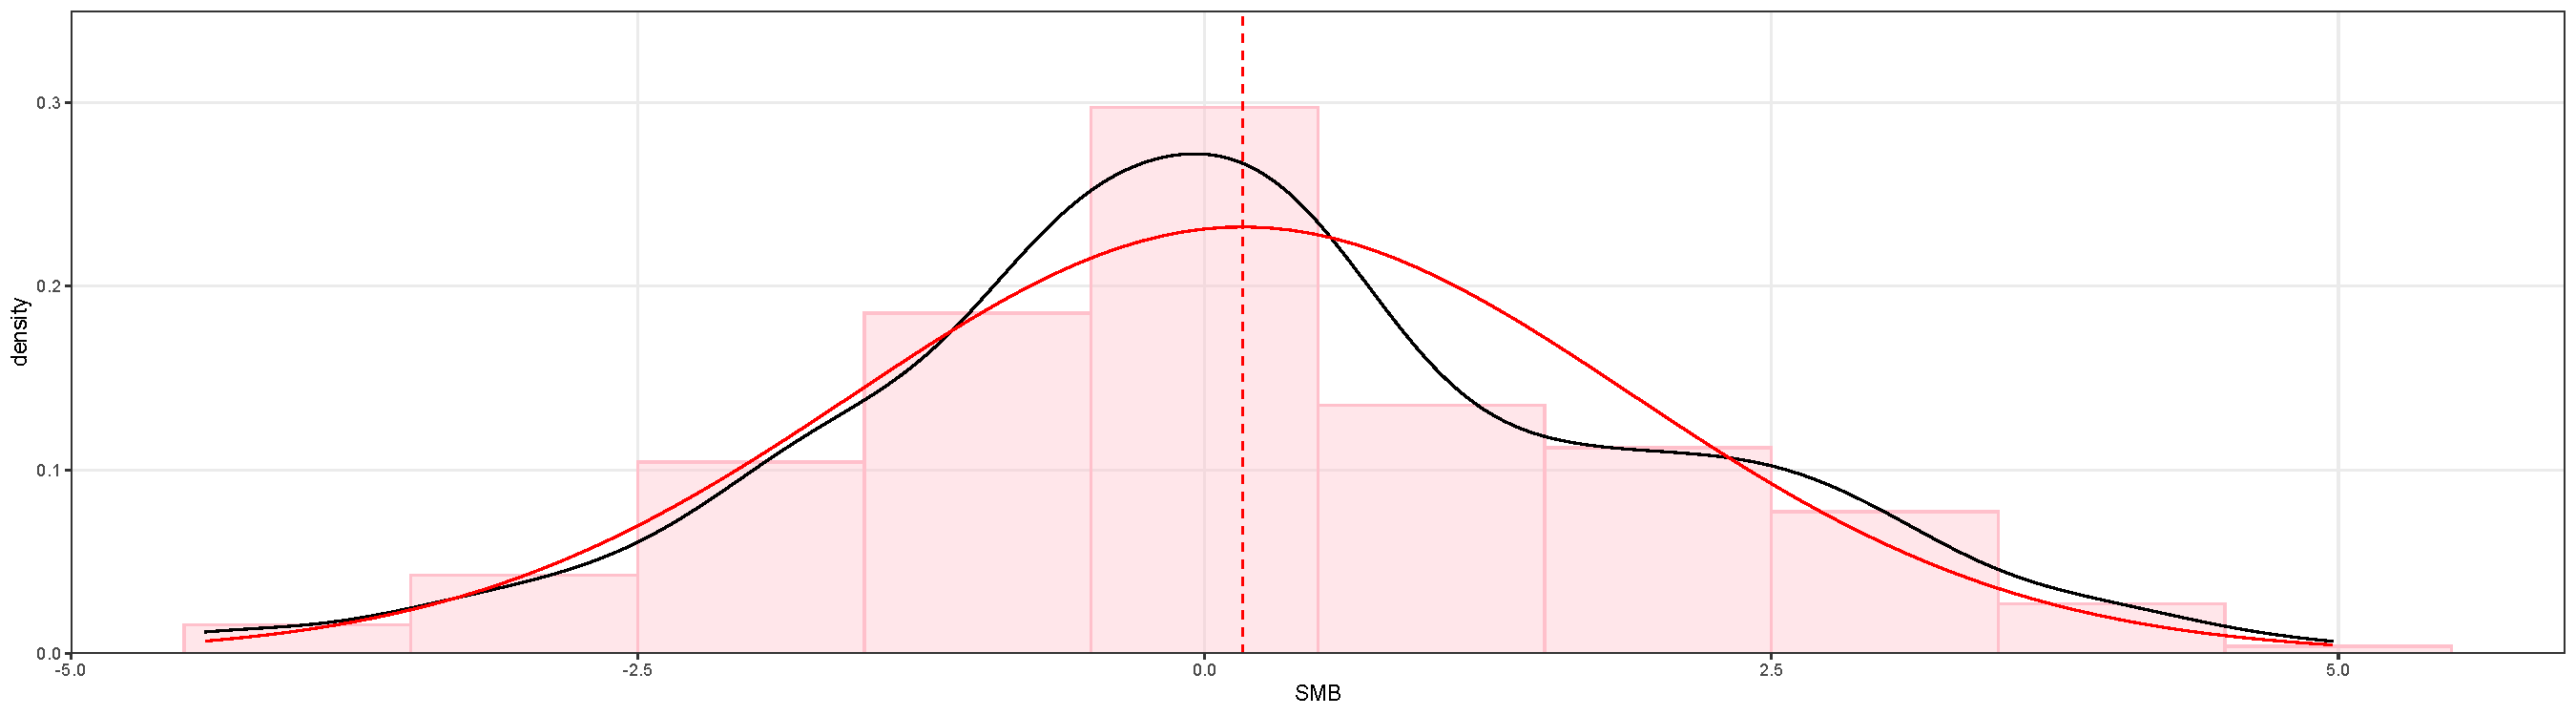
\includegraphics[width=1\linewidth]{Master_Thesis_Andreas_Kracht_Frandsen_files/figure-latex/SMB-HIST-1} 

}

\caption{Autokorrelation af log netto renten.}\label{fig:SMB-HIST}
\end{figure}

\hypertarget{nominel-rente-x_ttextb}{%
\subsection{\texorpdfstring{Nominel rente -- \(x_t^{\text{b}}\)}{Nominel rente -- x\_t\^{}\{\textbackslash text\{b\}\}}}\label{nominel-rente-x_ttextb}}

Det kvartalsvise log brutto afkast på den amerikanske 90-dages \emph{T-Bill} benyttes som en proxy for den nominelle rente. Ved at inkludere både brutto og netto log renten, inkorporeres inflation. Eftersom log inflation er forskellen mellem log brutto renten og log netto renten. Data er fra \citep{CRSPt90} og hentet gennem \citep{WRDSt90}. Den justerede middelværdi estimeres til 1.173\(\%\). Volatiliteten estimeres til 0.837\(\%\). Tredje og fjerde moment estimeres til hhv. 0.903 og 4.313. Figur \ref{fig:B-tids} viser et plot over tidsserien.

\begin{figure}[htbp!]

{\centering 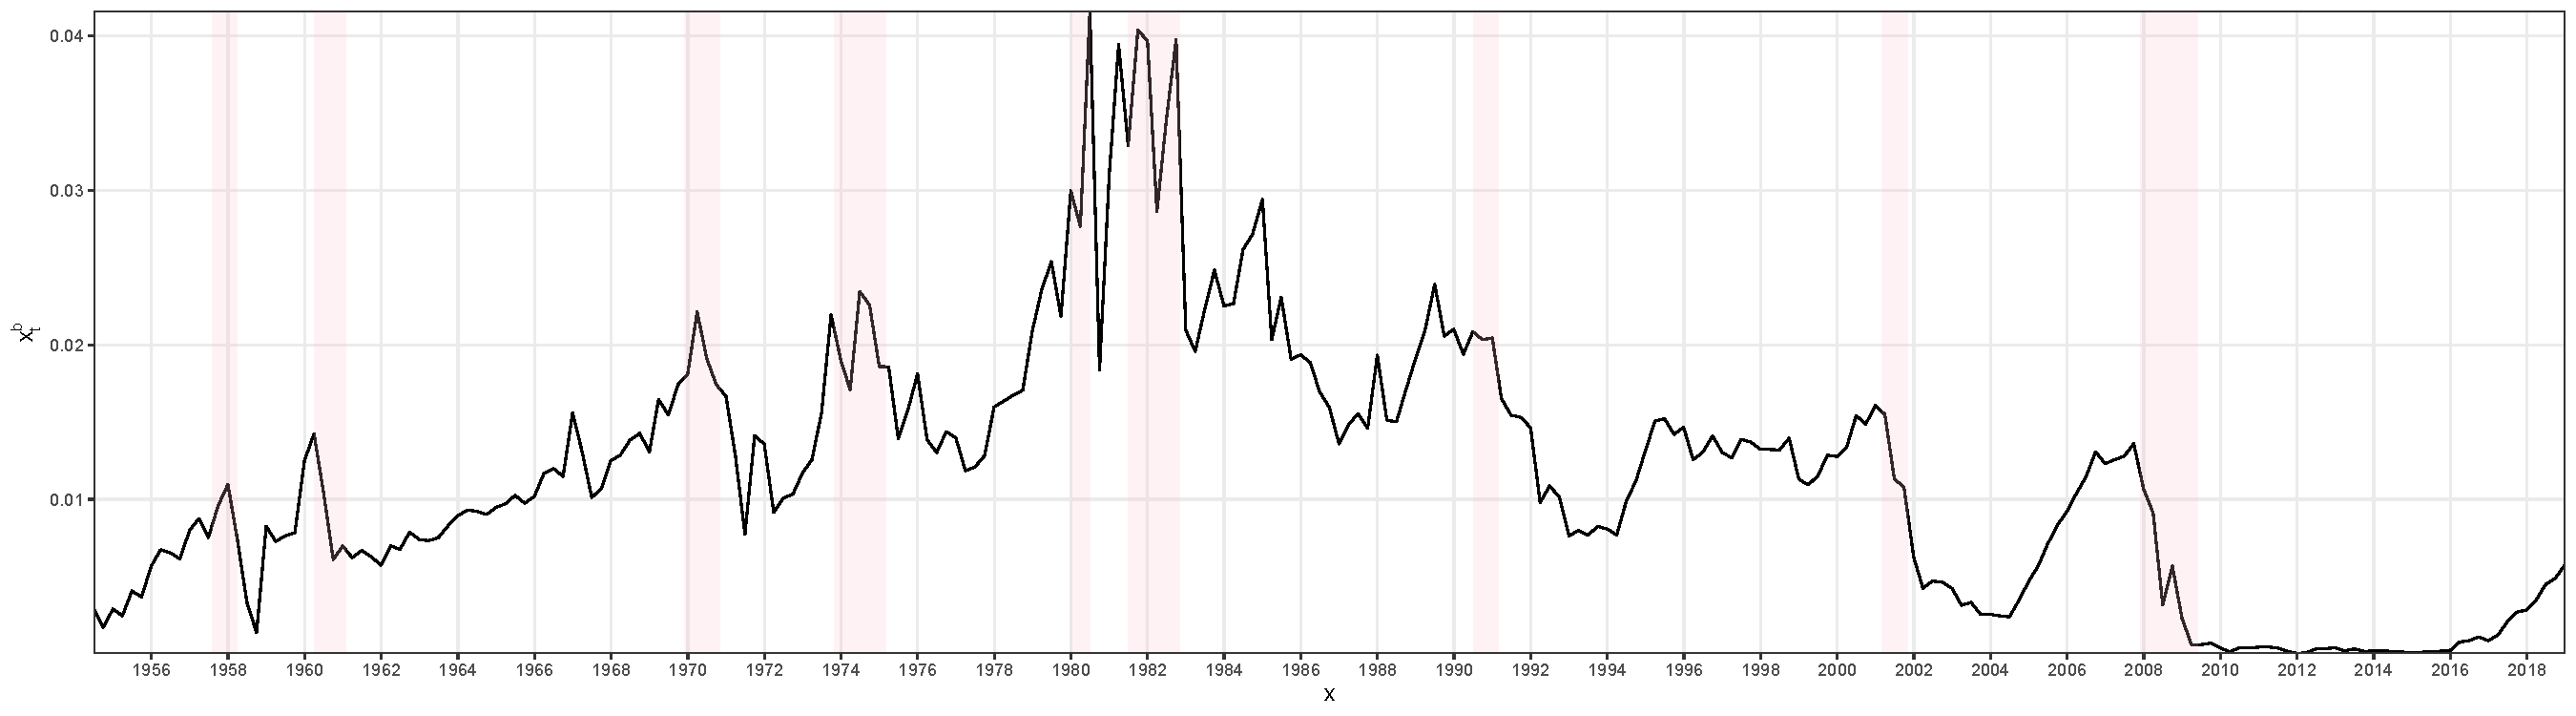
\includegraphics[width=1\linewidth]{Master_Thesis_Andreas_Kracht_Frandsen_files/figure-latex/B-tids-1} 

}

\caption{Tidsserie af log brutto afkastet på det risikofrie aktiv.}\label{fig:B-tids}
\end{figure}

\begin{figure}[htbp!]

{\centering 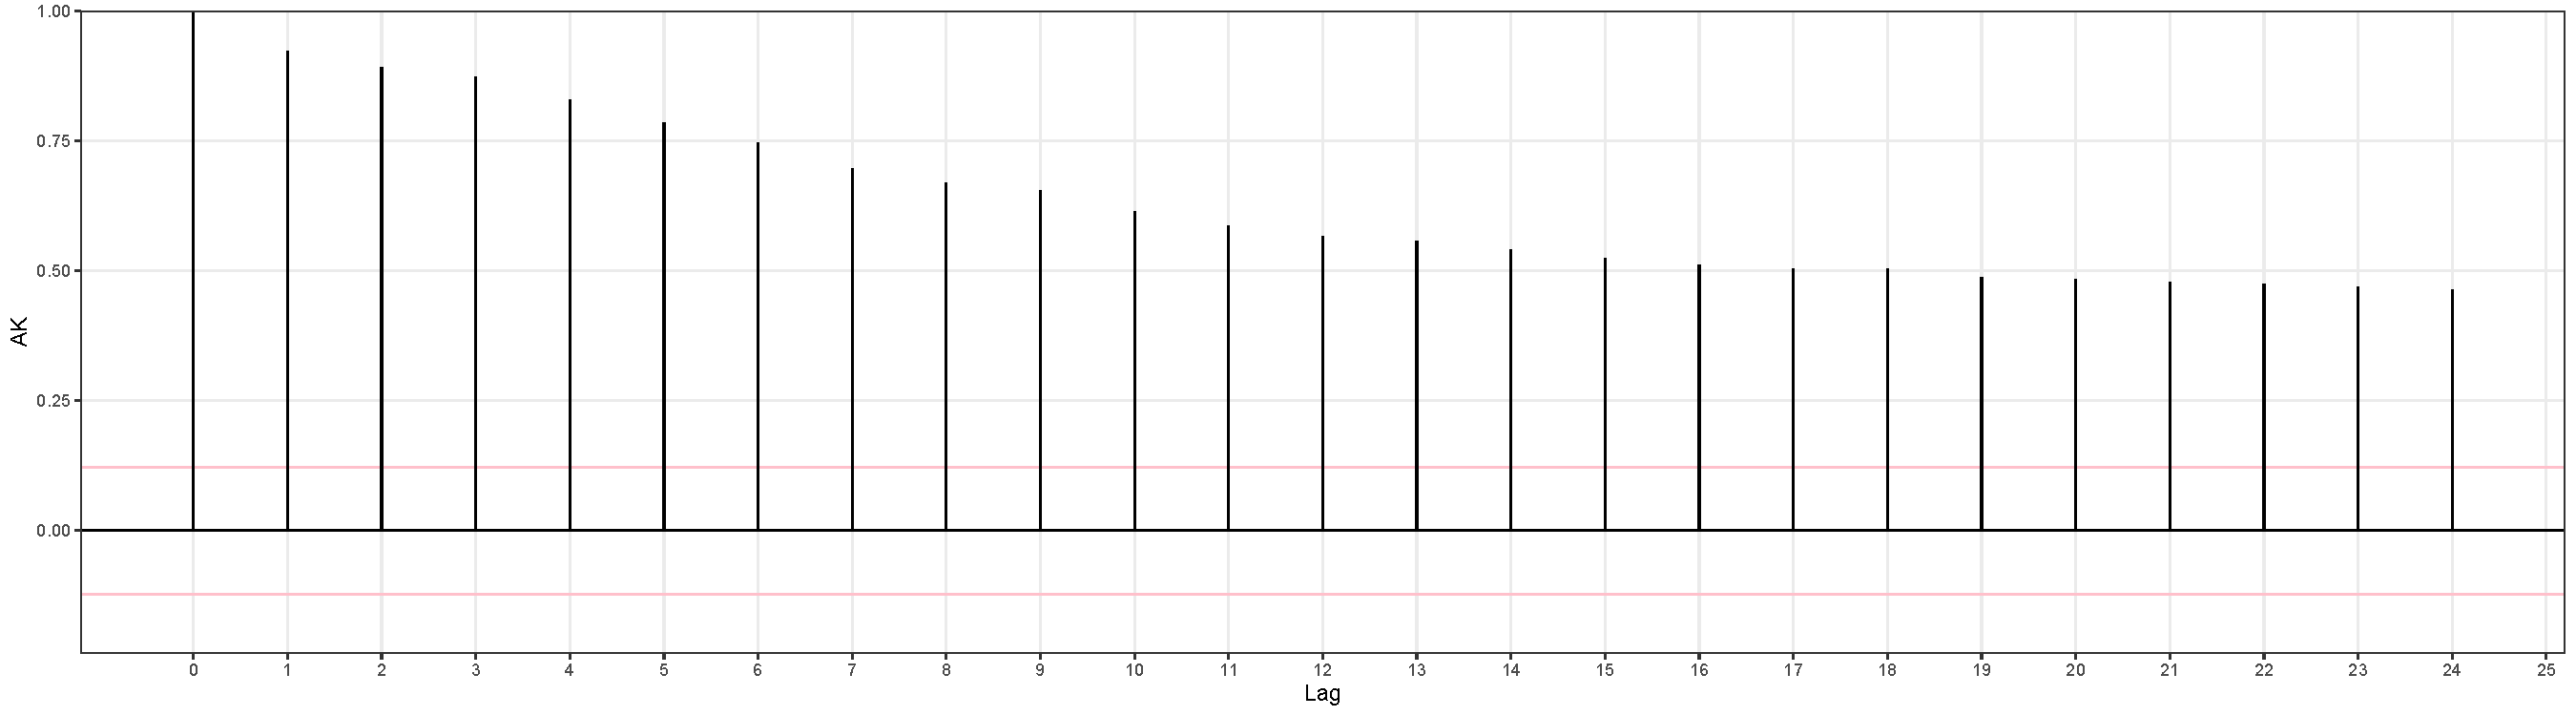
\includegraphics[width=1\linewidth]{Master_Thesis_Andreas_Kracht_Frandsen_files/figure-latex/B-AK-1} 

}

\caption{Autokorrelation af log merafkastet af virksomhedsobligationer.}\label{fig:B-AK}
\end{figure}

\begin{figure}[htbp!]

{\centering 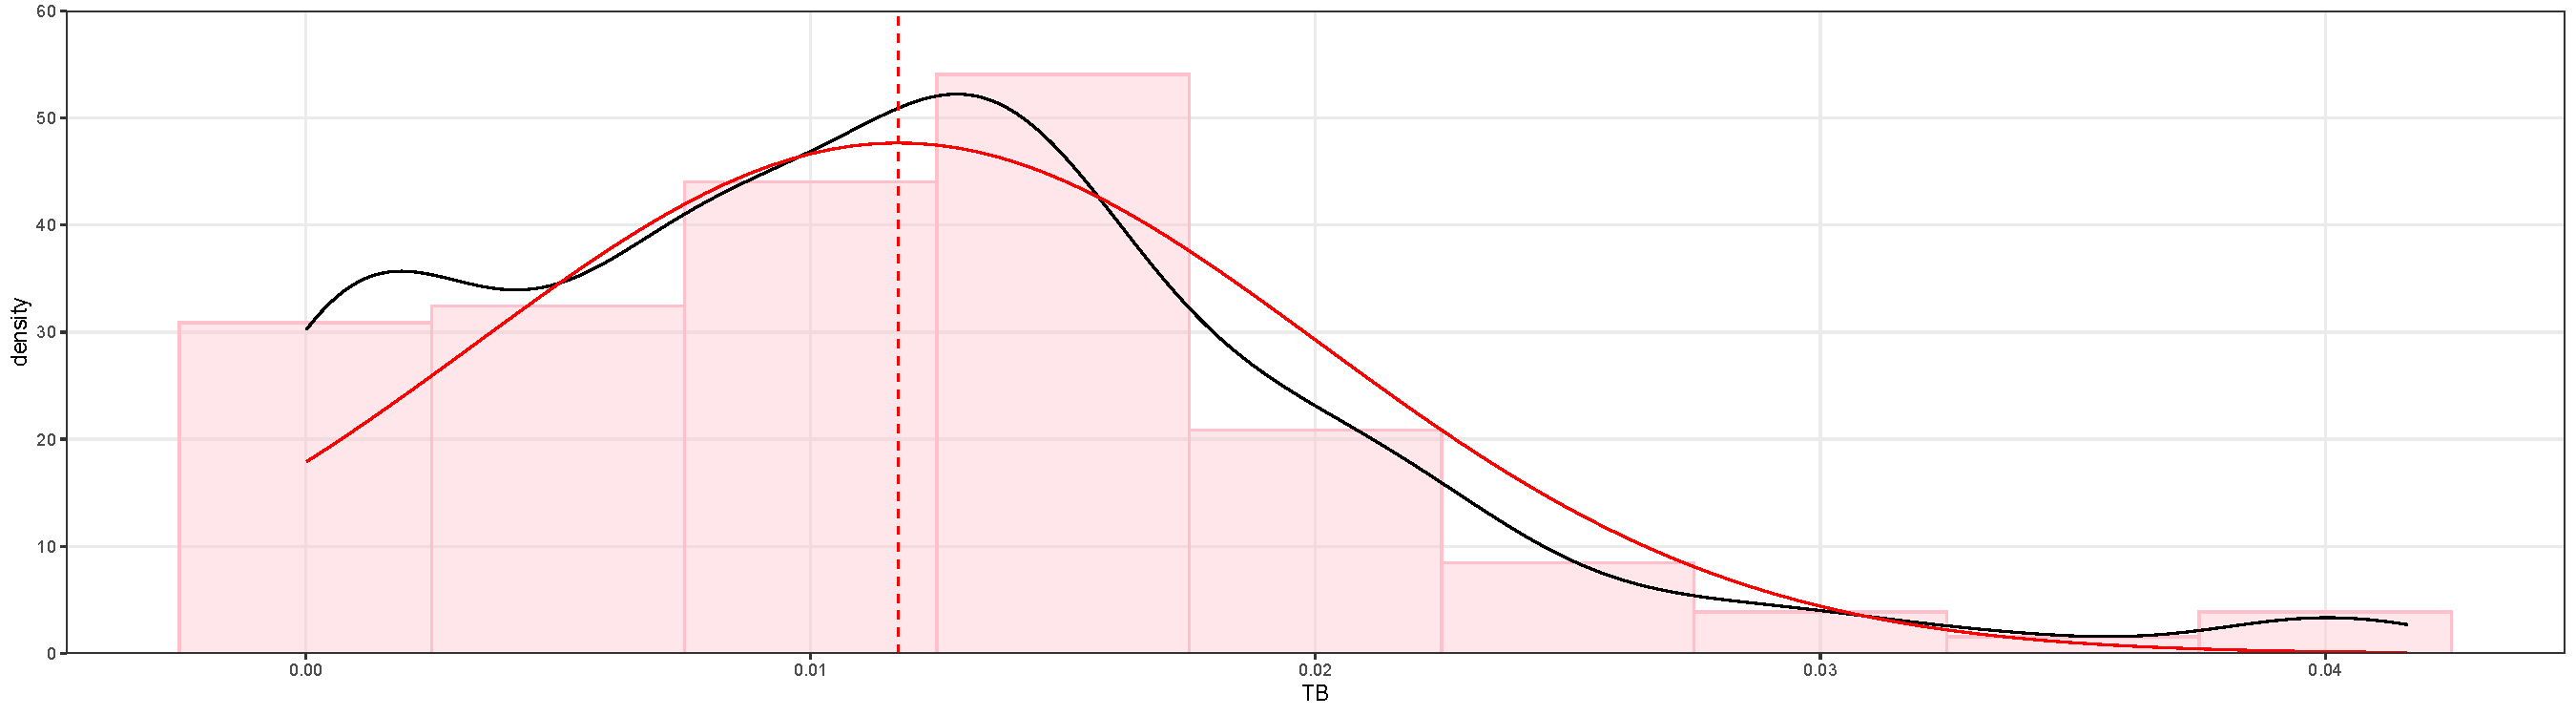
\includegraphics[width=1\linewidth]{Master_Thesis_Andreas_Kracht_Frandsen_files/figure-latex/B-HIST-1} 

}

\caption{Autokorrelation af log netto renten.}\label{fig:B-HIST}
\end{figure}

\hypertarget{term-spread-x_ttextts}{%
\subsection{\texorpdfstring{Term Spread -- \(x_t^{\text{ts}}\)}{Term Spread -- x\_t\^{}\{\textbackslash text\{ts\}\}}}\label{term-spread-x_ttextts}}

For at beregne \emph{Term Spread} (rentespændet for den lange rente), benyttes den amerikanske \(10\)-årige effektive rente med konstant løbetid samt den 90-dages \emph{T-Bill} \emph{Secondary Market Rate}. Kvartalsvise data er hentet fra \citep{FRED102020} og \citep{FRED902020}, derudover er data ikke blevet sæsonjusteret. Spændet beregnes da som
\[x_t^{\text{ts}}=Y_t^{10}-Y_t^{90},\]

hvor \(Y_t^{10}\) og \(Y_t^{90}\) er de to effektive renter. Dette følger metoden fra \citep{Campbell1991}, som også argumenterer for, at ethvert rentespænd for renter med løbetider mellem \(1\) måned og \(10\) år, kan prædiktere rentestrukturen. Middelværdien for det lange rentespænd estimeres til 1.469\(\%\). Volatiliteten estimeres til 1.186\(\%\). Fordelingen er forholdsvis symmetrisk med skævhed og kurtosis på hhv. -0.231 og 3.033. Figur \ref{fig:TS-tids} viser et plot over tidsserien.

\begin{figure}[htbp!]

{\centering 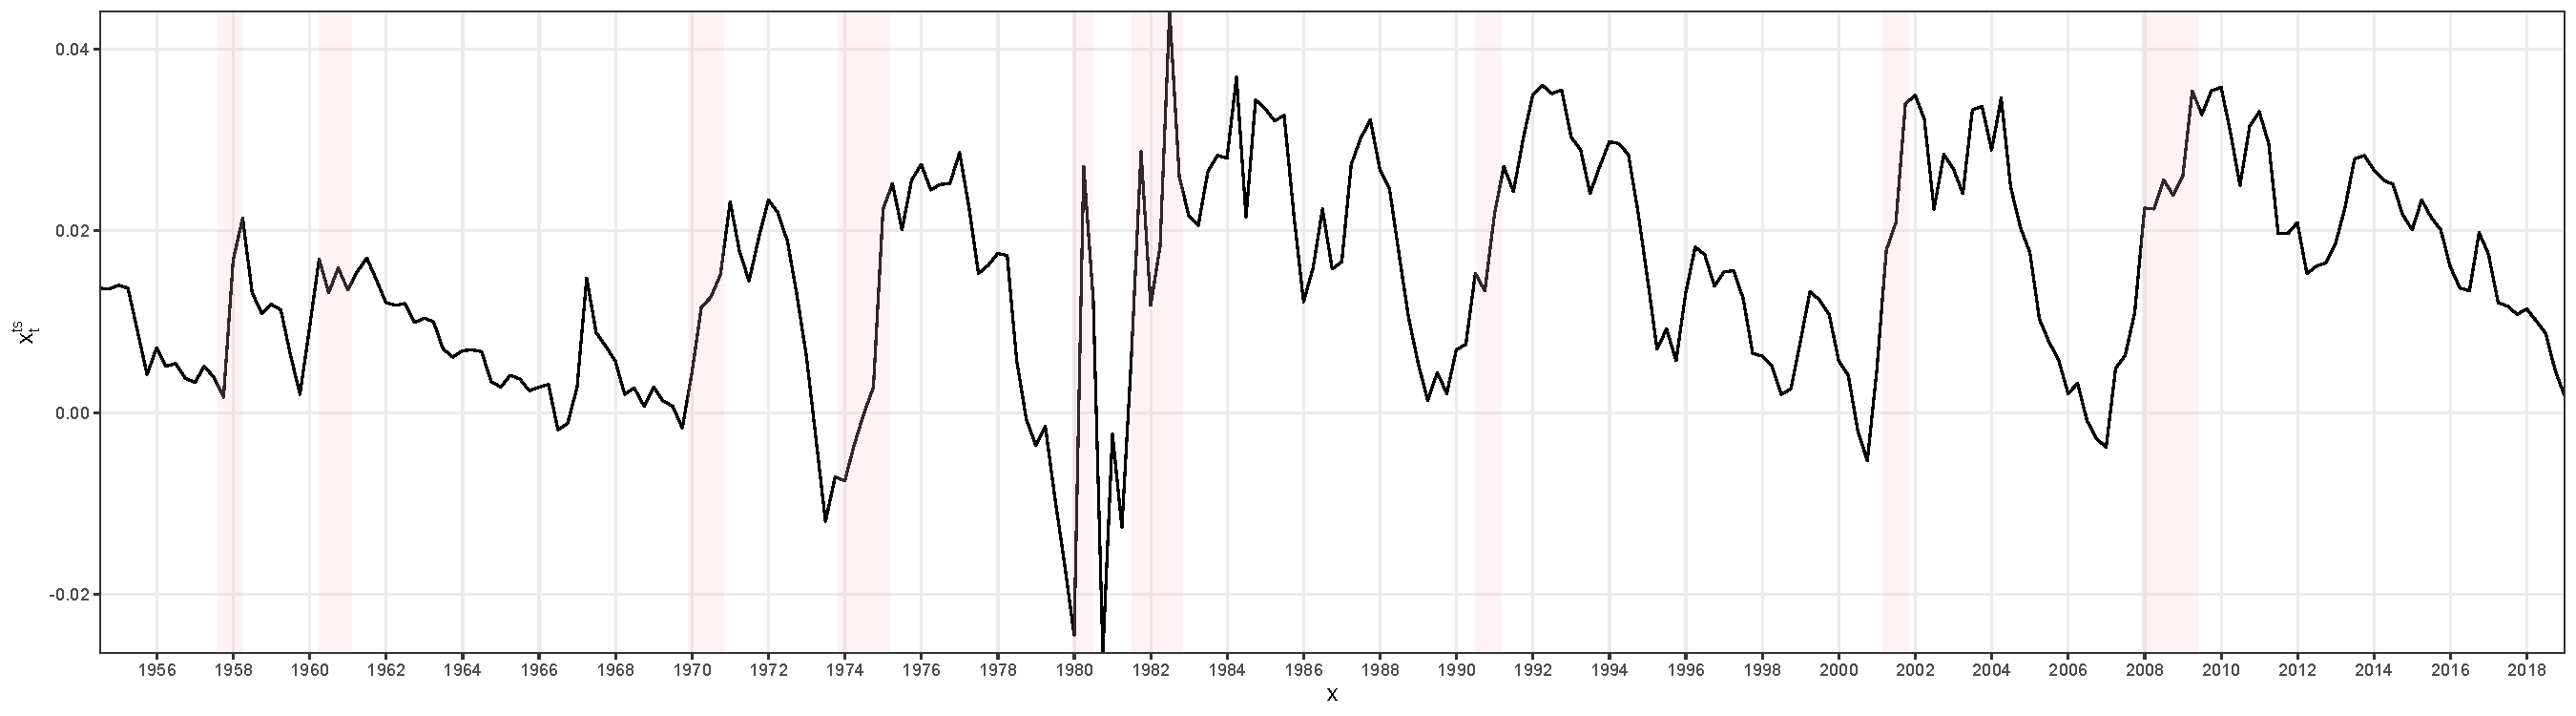
\includegraphics[width=1\linewidth]{Master_Thesis_Andreas_Kracht_Frandsen_files/figure-latex/TS-tids-1} 

}

\caption{Tidsserie af Term Spread.}\label{fig:TS-tids}
\end{figure}

\begin{figure}[htbp!]

{\centering 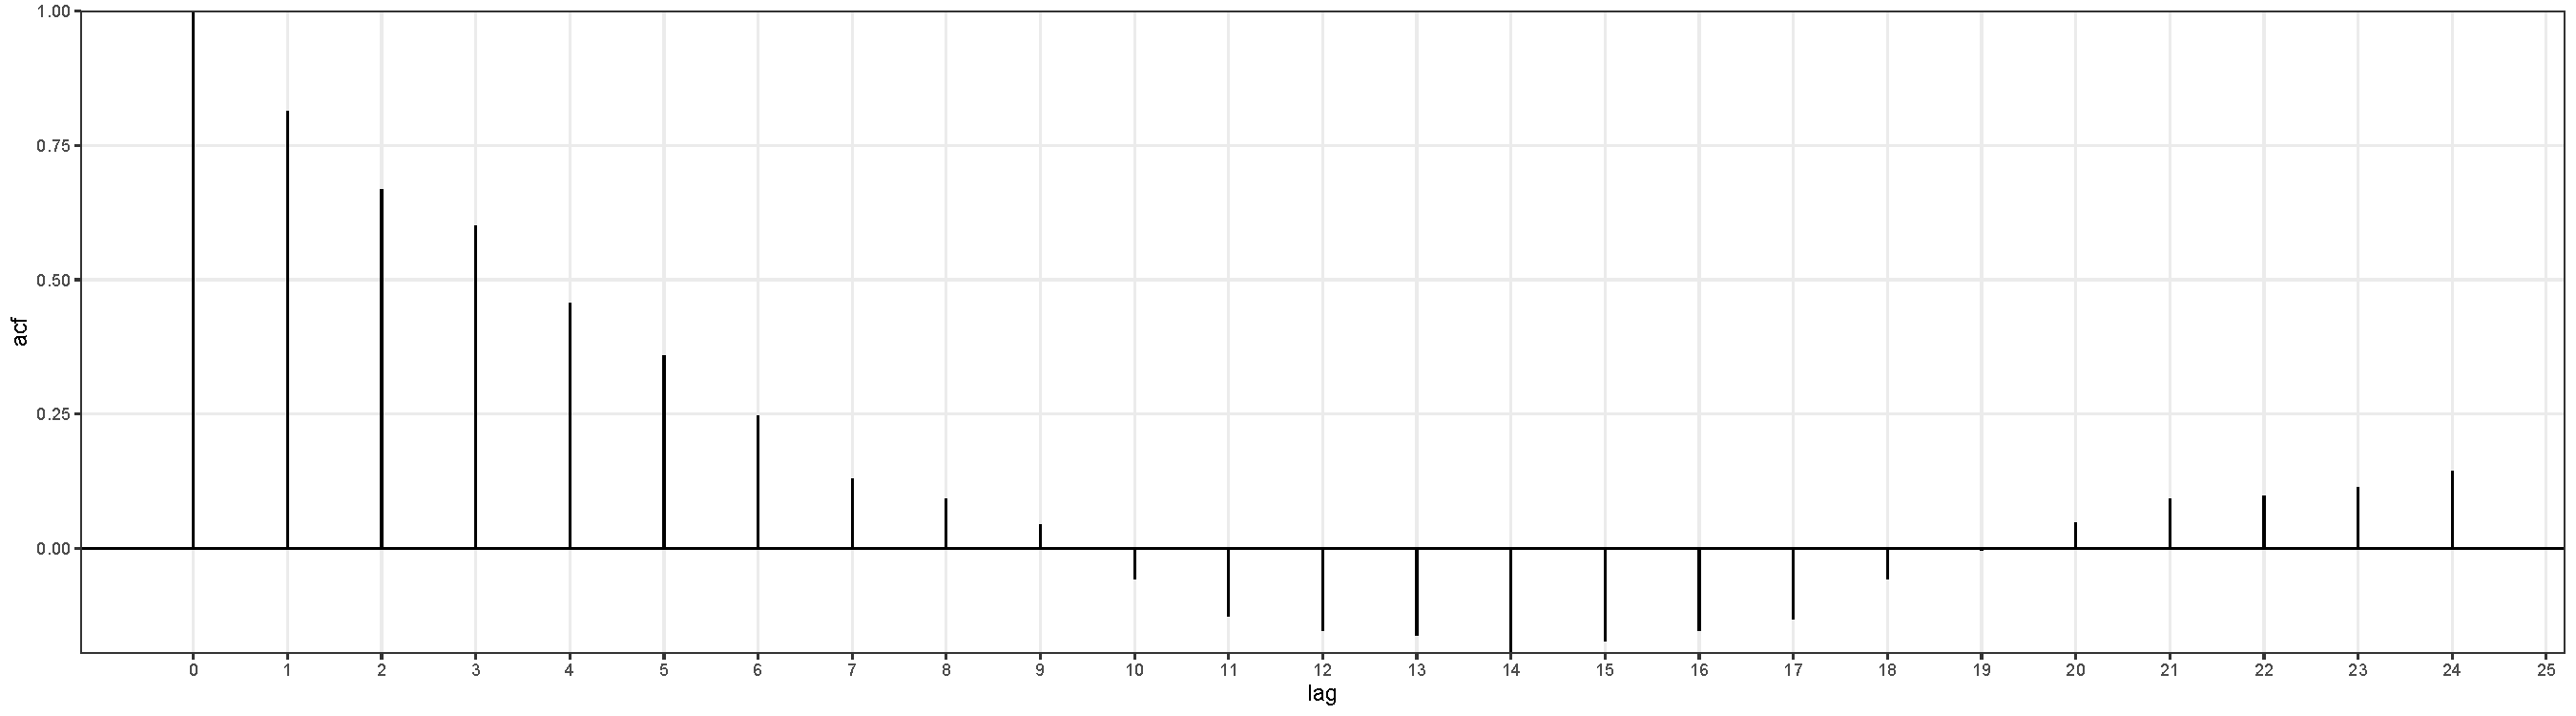
\includegraphics[width=1\linewidth]{Master_Thesis_Andreas_Kracht_Frandsen_files/figure-latex/TS-AK-1} 

}

\caption{Autokorrelation af log merafkastet af virksomhedsobligationer.}\label{fig:TS-AK}
\end{figure}

\begin{figure}[htbp!]

{\centering 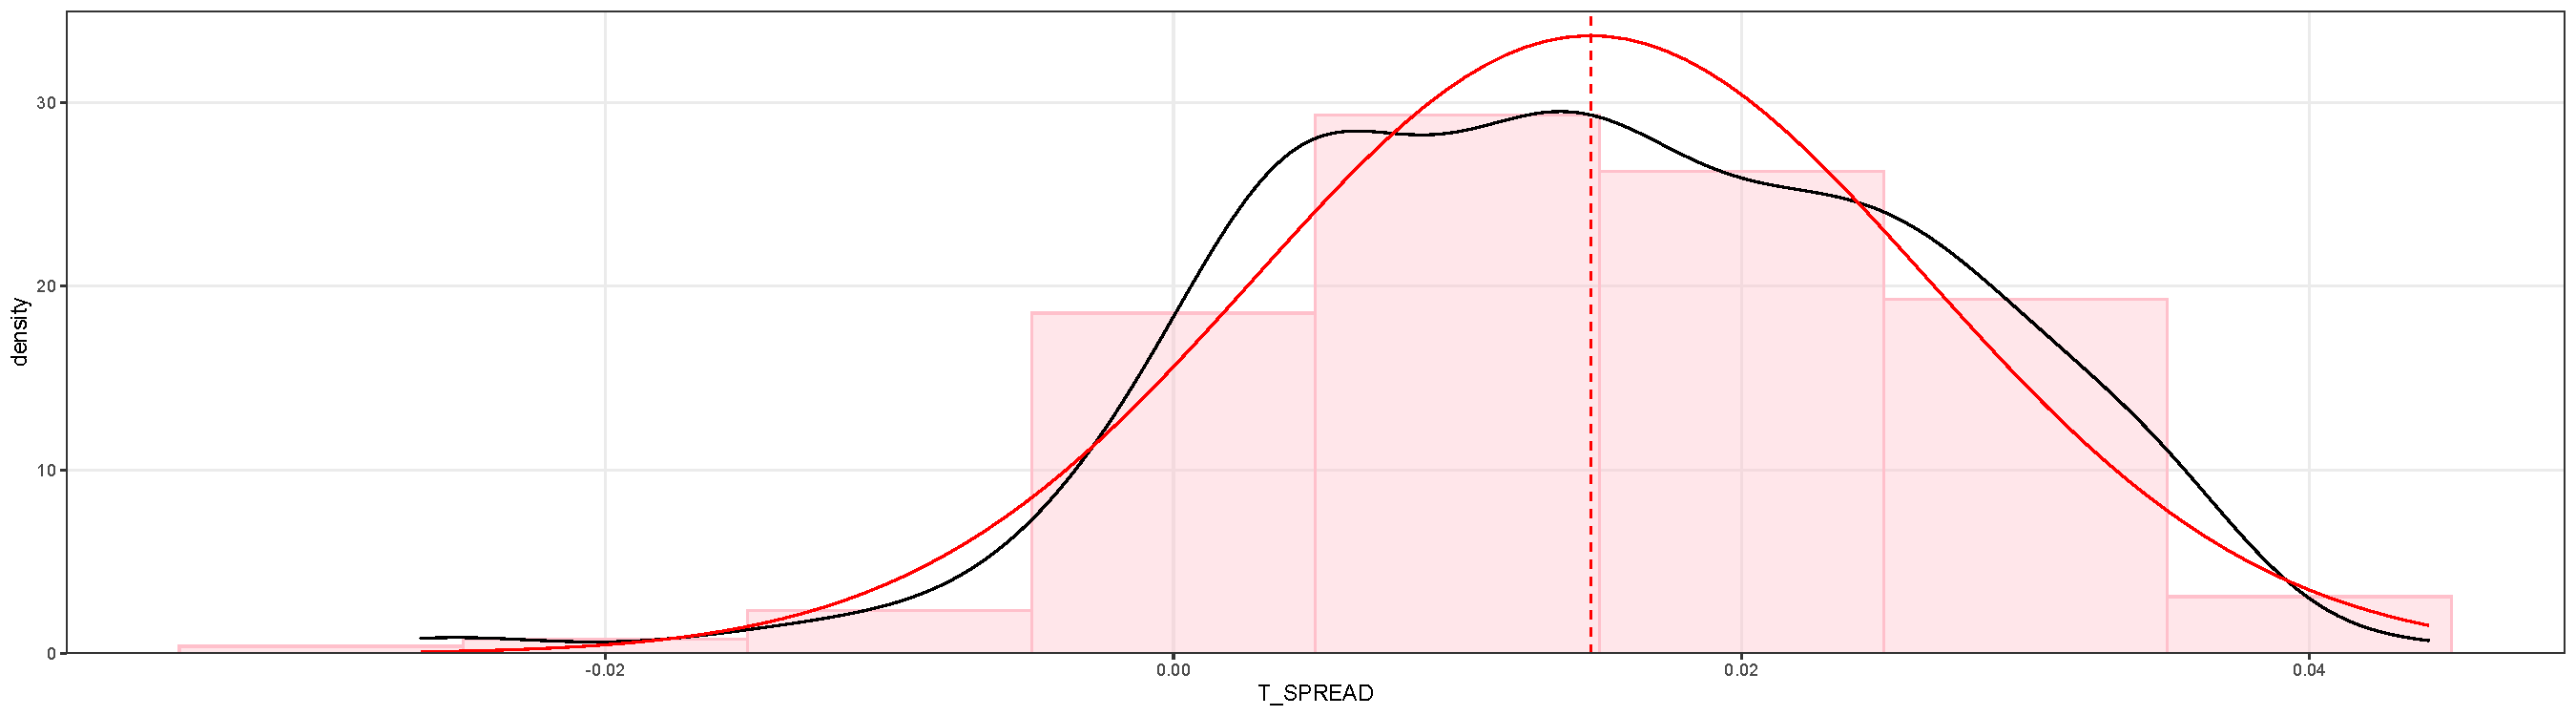
\includegraphics[width=1\linewidth]{Master_Thesis_Andreas_Kracht_Frandsen_files/figure-latex/TS-HIST-1} 

}

\caption{Autokorrelation af log netto renten.}\label{fig:TS-HIST}
\end{figure}

\hypertarget{yield-spread-x_ttextys}{%
\subsection{\texorpdfstring{Yield Spread -- \(x_t^{\text{ys}}\)}{Yield Spread -- x\_t\^{}\{\textbackslash text\{ys\}\}}}\label{yield-spread-x_ttextys}}

Datagrundlaget for \emph{Yield Spread} (rentespændet for den korte rente) er den amerikanske \(10\)-årige effektive rente med konstant løbetid samt den 90-dages \emph{T-Bill} \emph{Secondary Market Rate}. Kvartalsvise data er hentet fra \citep{FRED52020} og \citep{FRED902020}, og er ikke sæsonjusteret. Spændet beregnes da som
\[x_t^{\text{ts}}=Y_t^{5}-Y_t^{90},\]

hvor \(Y_t^{5}\) og \(Y_t^{90}\) er de to effektive renter. Middelværdien, 1.166\(\%\), er som forventet en anelse mindre end middelværdien for \emph{Term Spread}. Det samme er volatiliteten, 0.927\(\%\). Fordelingen er en anelse leptokurtisk med kurtosis på 3.828. Skævheden er -0.153. Figur \ref{fig:YS-tids} viser et plot over tidsserien.

\begin{figure}[htbp!]

{\centering 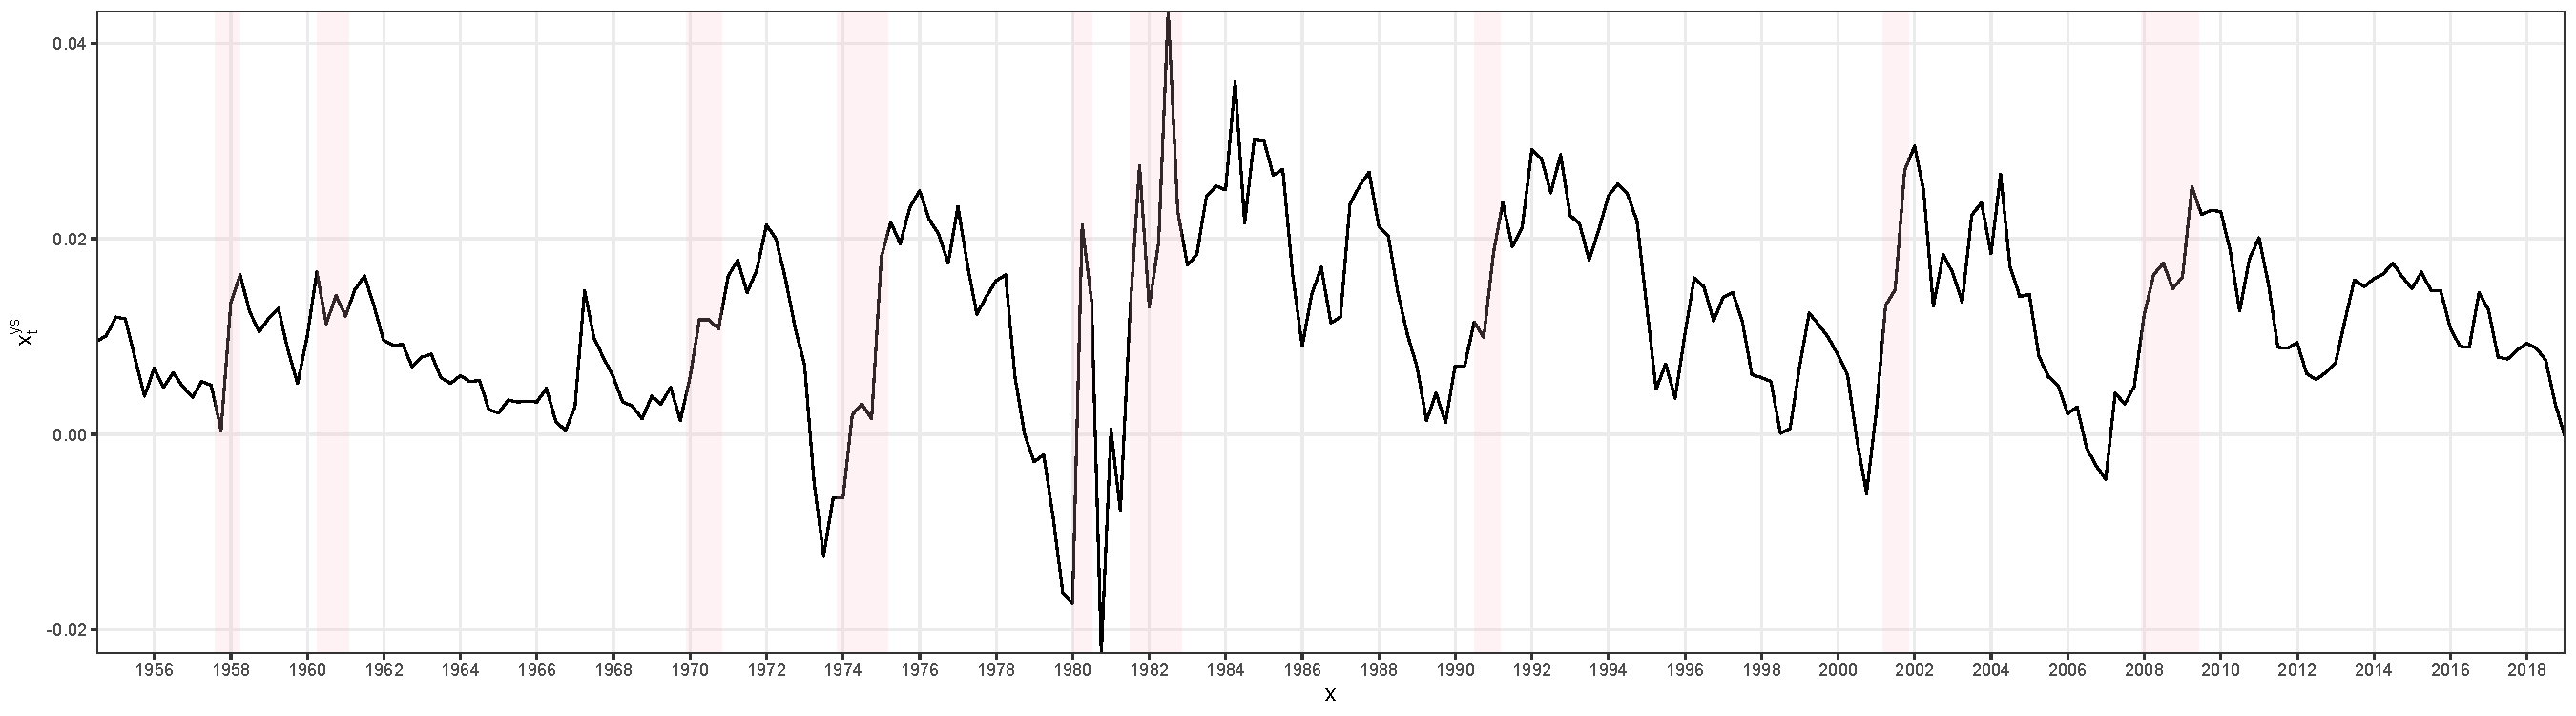
\includegraphics[width=1\linewidth]{Master_Thesis_Andreas_Kracht_Frandsen_files/figure-latex/YS-tids-1} 

}

\caption{Tidsserie af Yield Spread.}\label{fig:YS-tids}
\end{figure}

\begin{figure}[htbp!]

{\centering 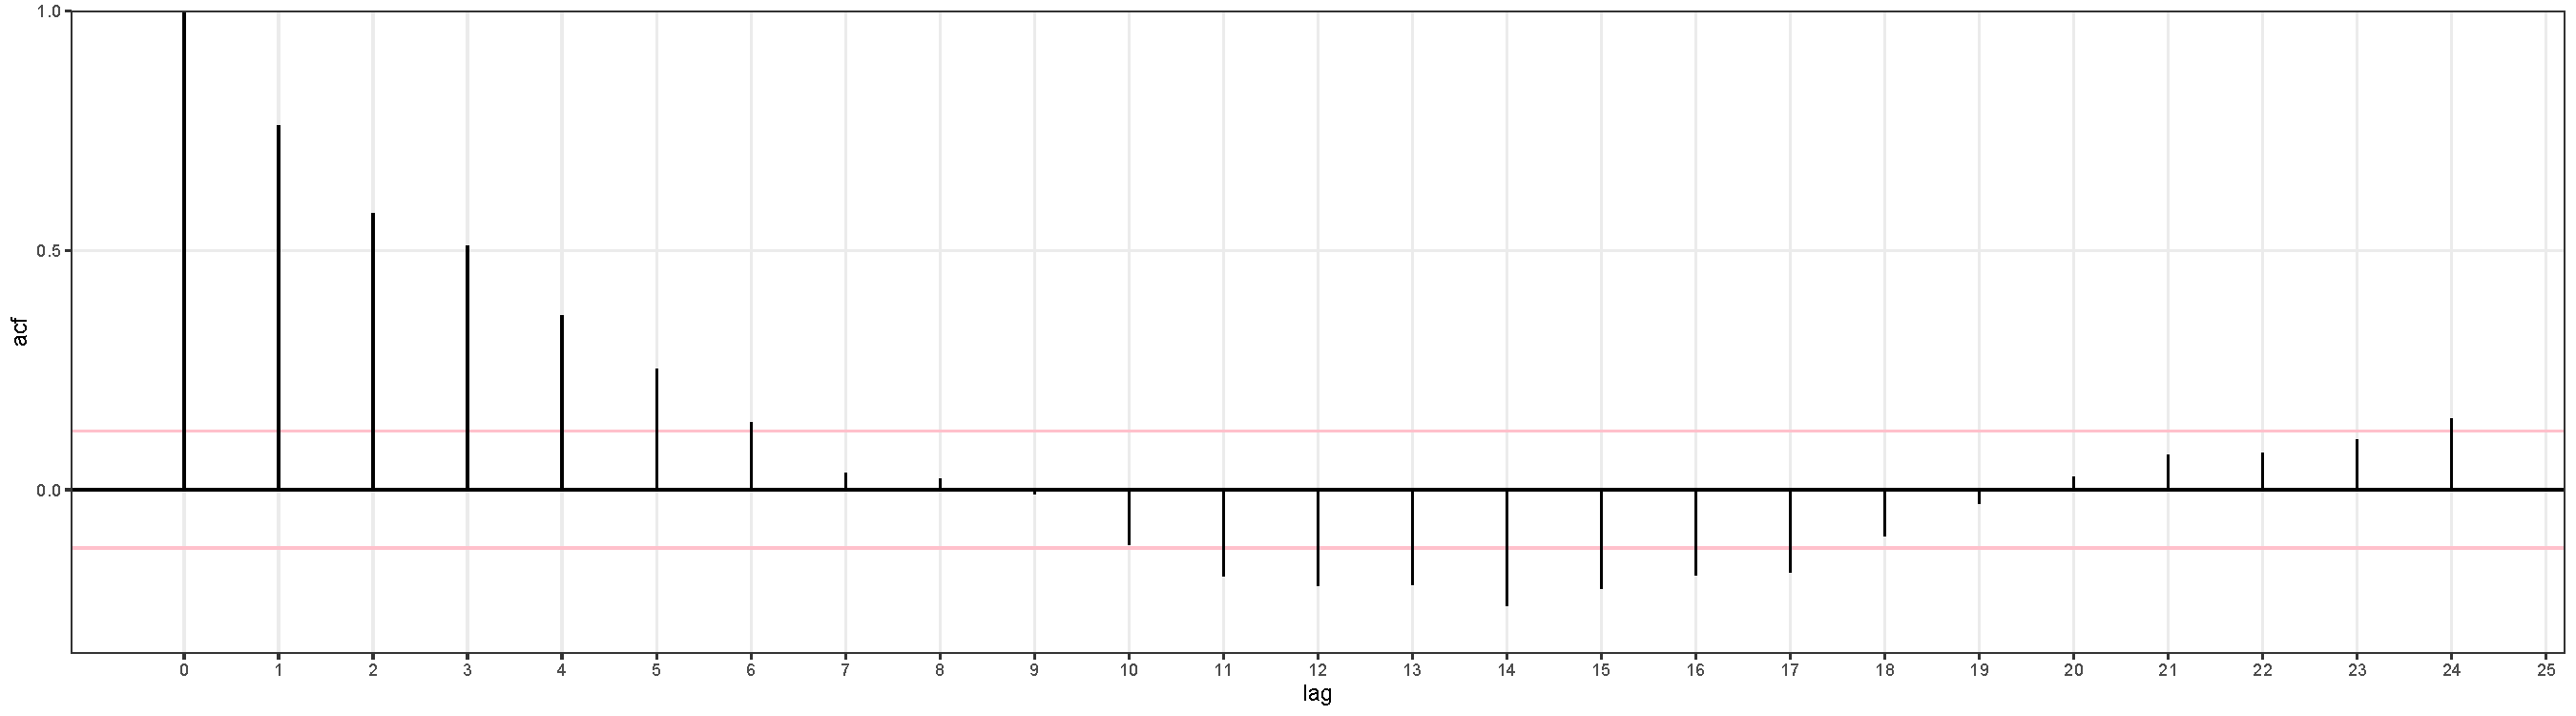
\includegraphics[width=1\linewidth]{Master_Thesis_Andreas_Kracht_Frandsen_files/figure-latex/YS-AK-1} 

}

\caption{Autokorrelation af log merafkastet af virksomhedsobligationer.}\label{fig:YS-AK}
\end{figure}

\begin{figure}[htbp!]

{\centering 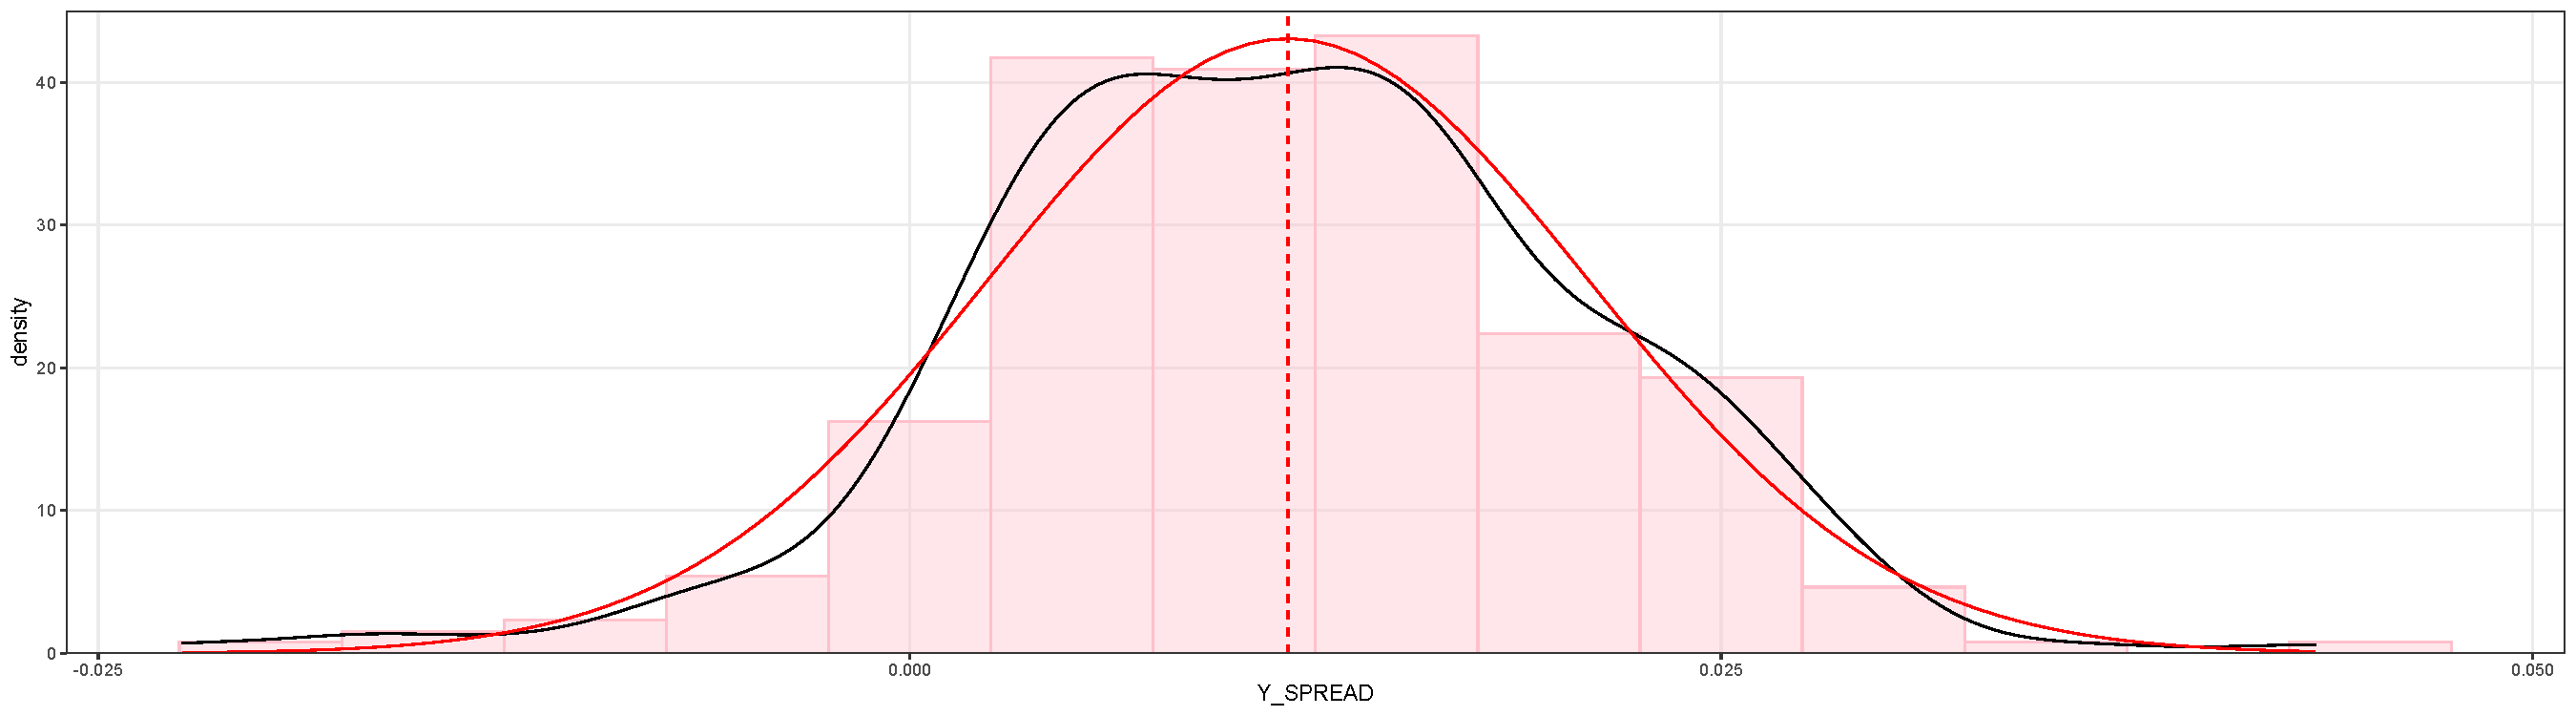
\includegraphics[width=1\linewidth]{Master_Thesis_Andreas_Kracht_Frandsen_files/figure-latex/YS-HIST-1} 

}

\caption{Autokorrelation af log netto renten.}\label{fig:YS-HIST}
\end{figure}

\hypertarget{credit-spread-x_ttextcs}{%
\subsection{\texorpdfstring{Credit Spread -- \(x_t^{\text{cs}}\)}{Credit Spread -- x\_t\^{}\{\textbackslash text\{cs\}\}}}\label{credit-spread-x_ttextcs}}

Beregningen til \emph{Credit Spread} (kreditspændet) benytter den 90-dages \emph{T-Bill} \emph{Secondary Market Rate} samt den effektive rente fra \emph{Moody's Seasoned BAA Corporate Bond}, og baserer sig på instrumenter med løbetider på \(20\) år eller mere. Data er hentet fra hhv. \citep{FRED902020} samt \citep{Goyal2007}. Metoden følger fra \citep{Keim1986}, og kreditspændet beregnes da som
\[x_t^{\text{cs}}=Y_t^{\text{BAA}}-Y_t^{90},\]

hvor \(Y_t^{\text{BAA}}\) og \(Y_t^{90}\) er de to effektive renter. Af de fem rentrestruktursvariable ses det, at kreditspændet har den højeste middelværdi på 3.398\(\%\), og en standardafvigelse på 1.732\(\%\). Tredje og fjerde moment estimeres til hhv. 0.159 og 2.33. Figur \ref{fig:CS-tids} viser et plot over tidsserien.

\begin{figure}[htbp!]

{\centering 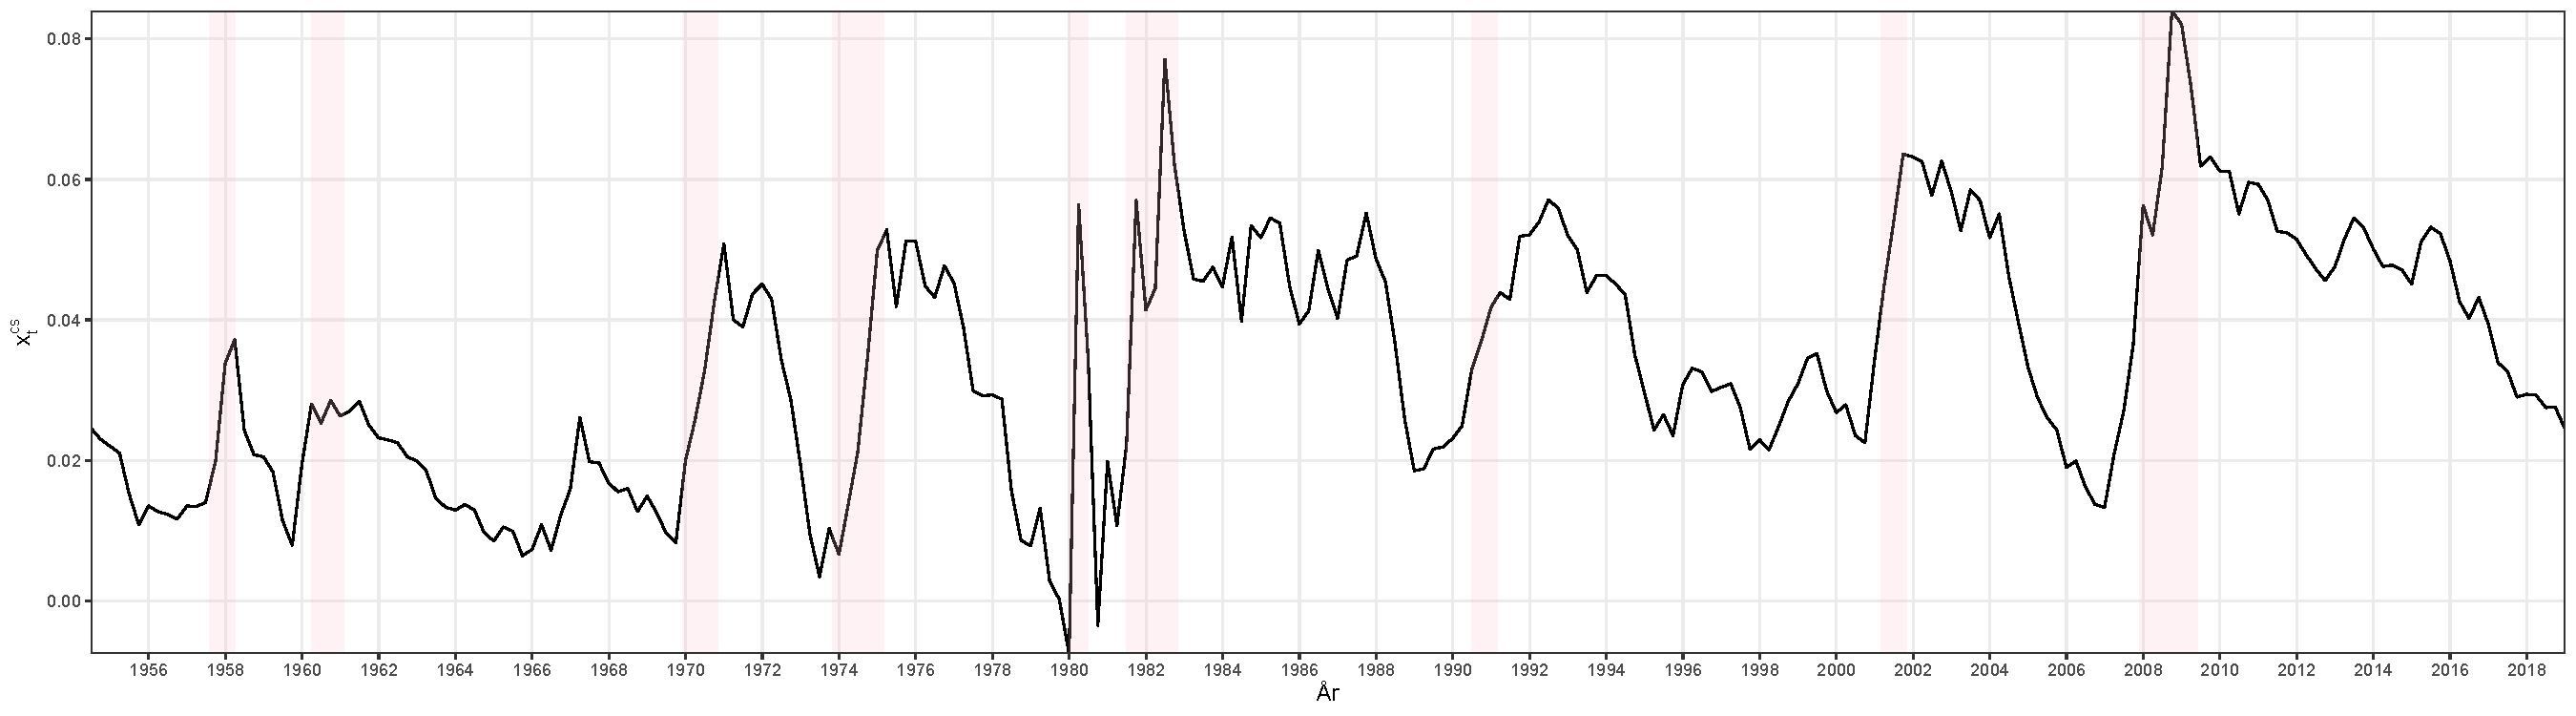
\includegraphics[width=1\linewidth]{Master_Thesis_Andreas_Kracht_Frandsen_files/figure-latex/CS-tids-1} 

}

\caption{Tidsserie af Credit Spread.}\label{fig:CS-tids}
\end{figure}

\begin{figure}[htbp!]

{\centering 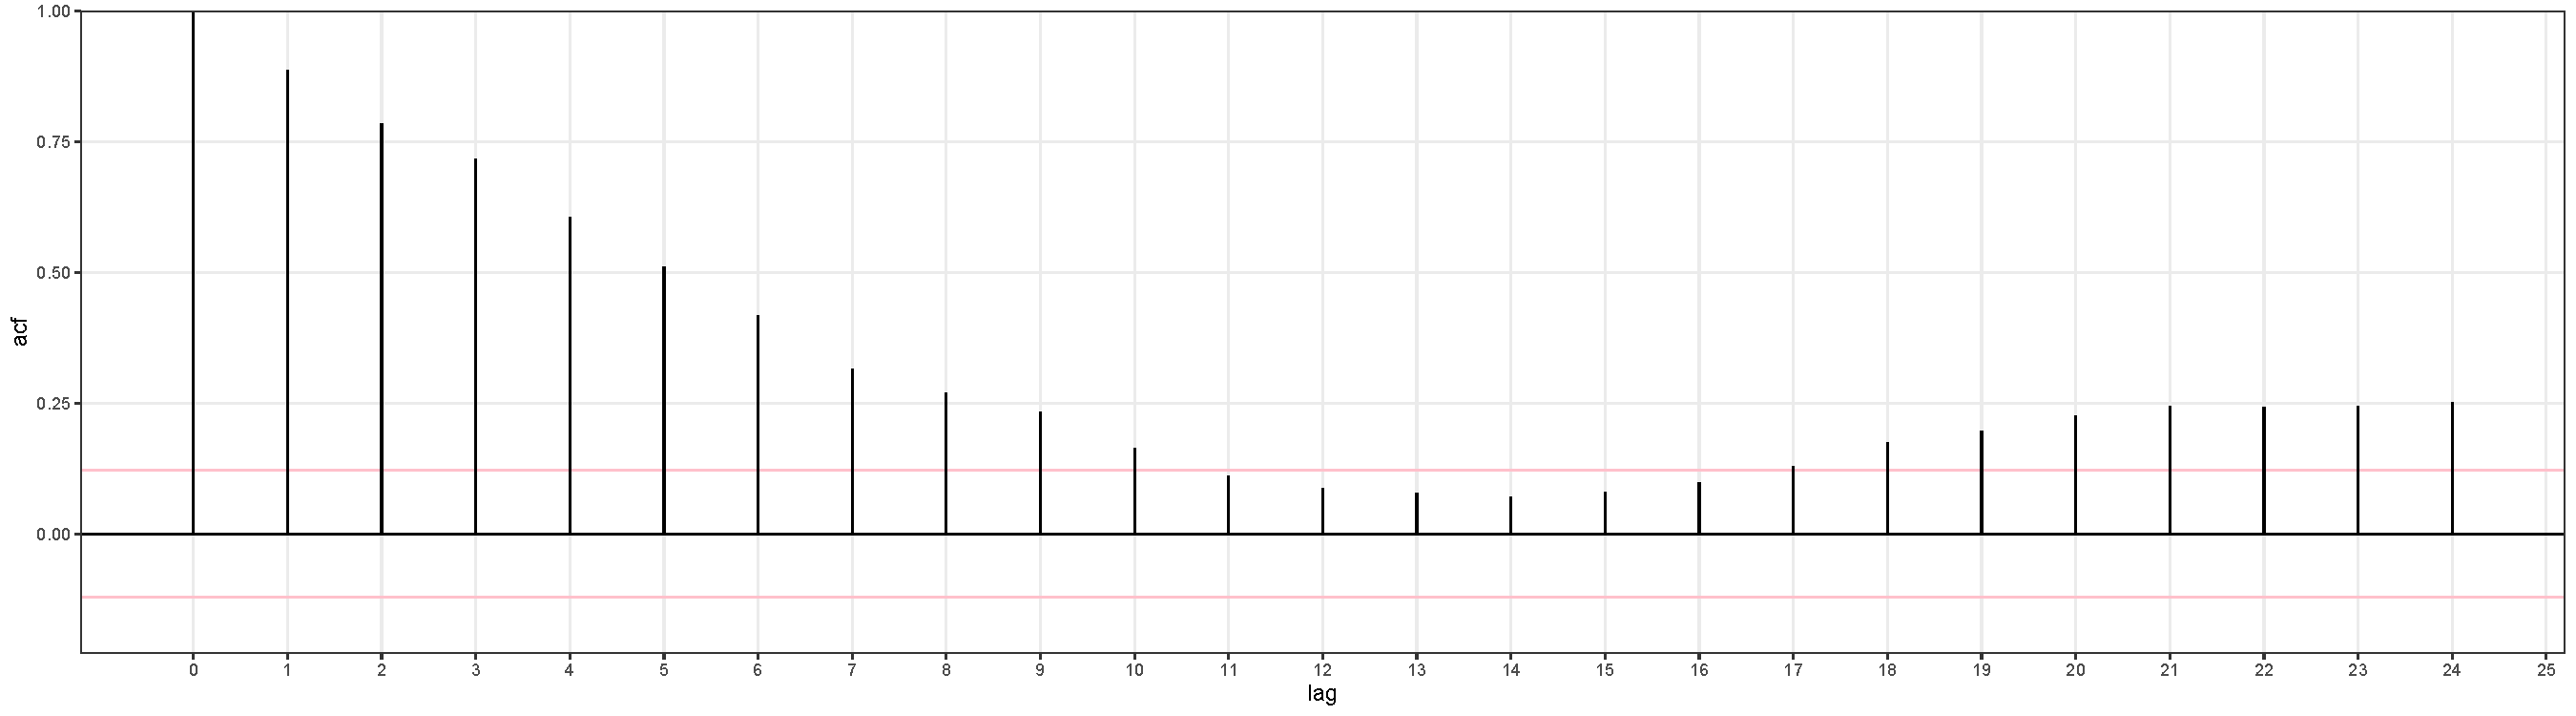
\includegraphics[width=1\linewidth]{Master_Thesis_Andreas_Kracht_Frandsen_files/figure-latex/CS-AK-1} 

}

\caption{Autokorrelation af log merafkastet af virksomhedsobligationer.}\label{fig:CS-AK}
\end{figure}

\begin{figure}[htbp!]

{\centering 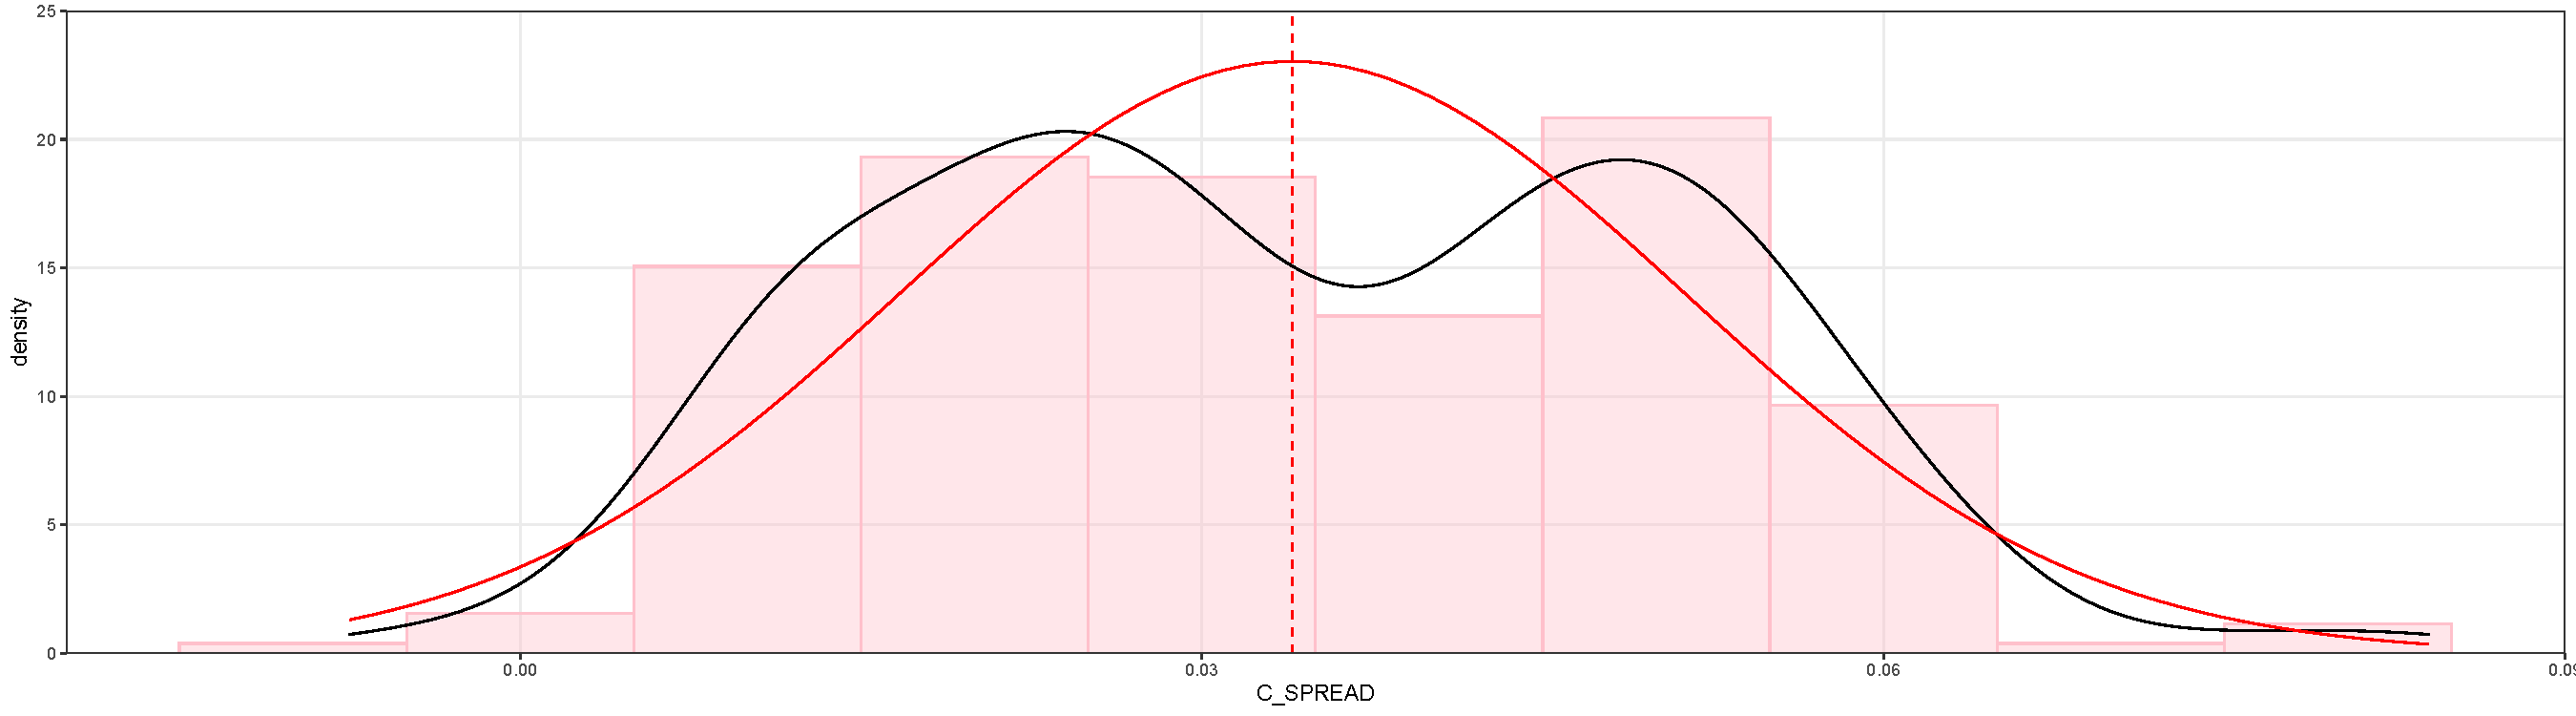
\includegraphics[width=1\linewidth]{Master_Thesis_Andreas_Kracht_Frandsen_files/figure-latex/CS-HIST-1} 

}

\caption{Autokorrelation af log netto renten.}\label{fig:CS-HIST}
\end{figure}

\hypertarget{default-spread-x_ttextds}{%
\subsection{\texorpdfstring{Default Spread -- \(x_t^{\text{ds}}\)}{Default Spread -- x\_t\^{}\{\textbackslash text\{ds\}\}}}\label{default-spread-x_ttextds}}

For at beregne \emph{Default Spread} (konkursspændet) benyttes den effektive rente fra \emph{Moody's Seasoned AAA Corporate Bond} samt den effektive rente fra \emph{Moody's Seasoned BAA Corporate Bond}, og baserer sig begge på instrumenter med løbetider på \(20\) år eller mere. Data er hentet via \citep{Goyal2007}. Konkursspændet beregnes da som
\[x_t^{\text{ds}}=Y_t^{\text{BAA}}-Y_t^{\text{AAA}},\]

hvor \(Y_t^{\text{BAA}}\) og \(Y_t^{\text{AAA}}\) er de to effektive renter. Til forskel for kreditspændet har konkursspændet den laveste middelværdi, 0.987\(\%\), også på tværs af de andre klasser af prædiktionsvariable. Standardafvigelsen er 0.439\(\%\). Af rentestruktursvariablene har konkursspændet også den hhv. mest ekstreme skævhed og kurtosis. Disse er hhv. 1.842 og 8.156, hvilket indebærer en højreskæv fordeling med tykke haler. Figur \ref{fig:DS-tids} viser et plot over tidsserien.

\begin{figure}[htbp!]

{\centering 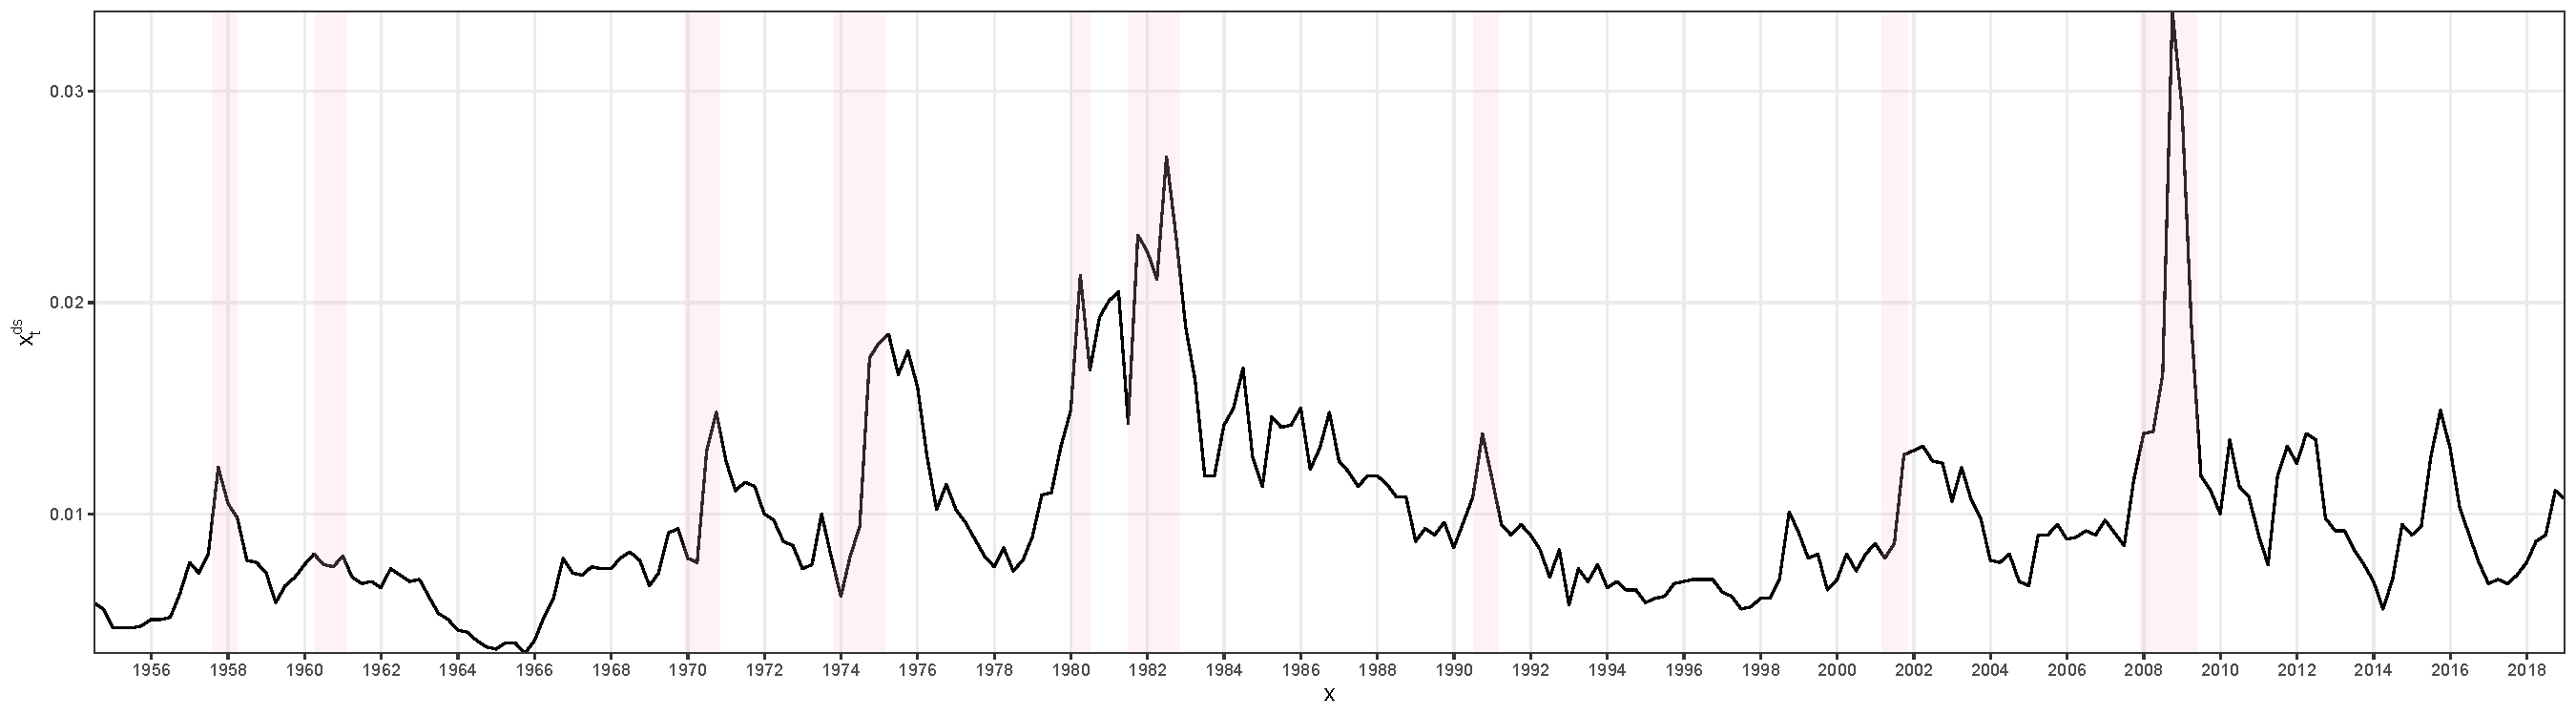
\includegraphics[width=1\linewidth]{Master_Thesis_Andreas_Kracht_Frandsen_files/figure-latex/DS-tids-1} 

}

\caption{Tidsserie af Default Spread.}\label{fig:DS-tids}
\end{figure}

\begin{figure}[htbp!]

{\centering 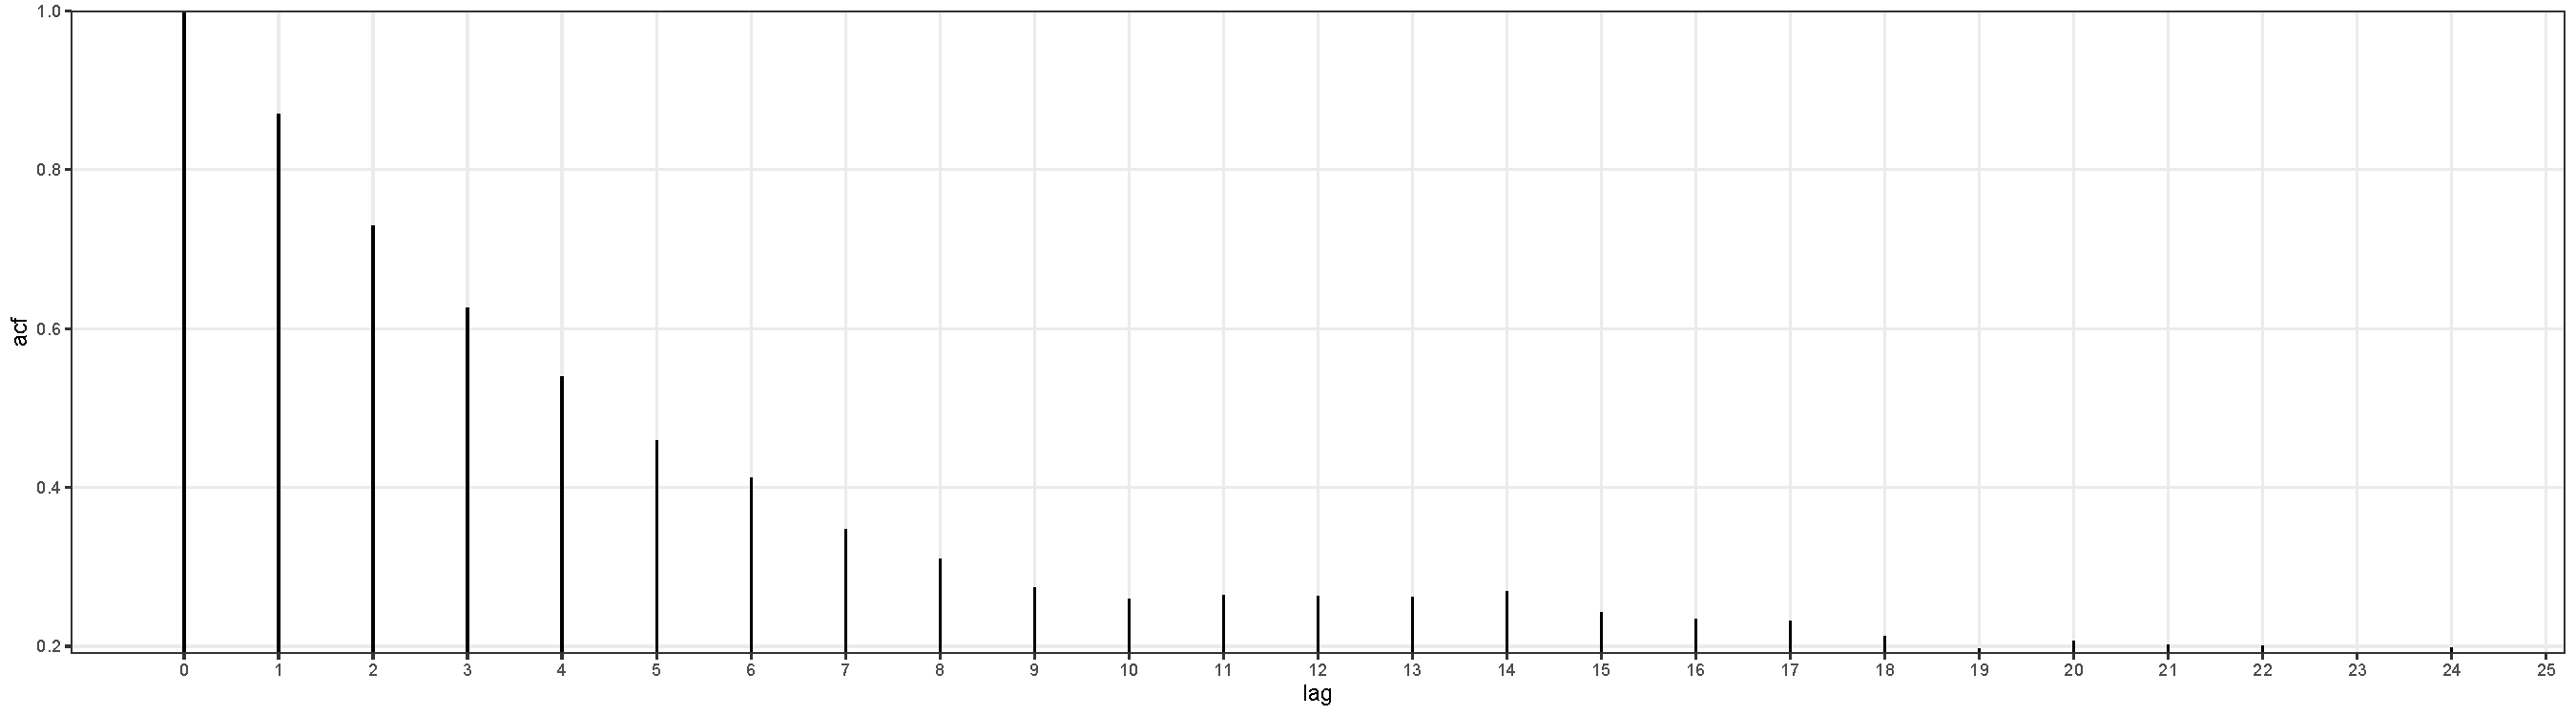
\includegraphics[width=1\linewidth]{Master_Thesis_Andreas_Kracht_Frandsen_files/figure-latex/DS-AK-1} 

}

\caption{Autokorrelation af log merafkastet af virksomhedsobligationer.}\label{fig:DS-AK}
\end{figure}

\begin{figure}[htbp!]

{\centering 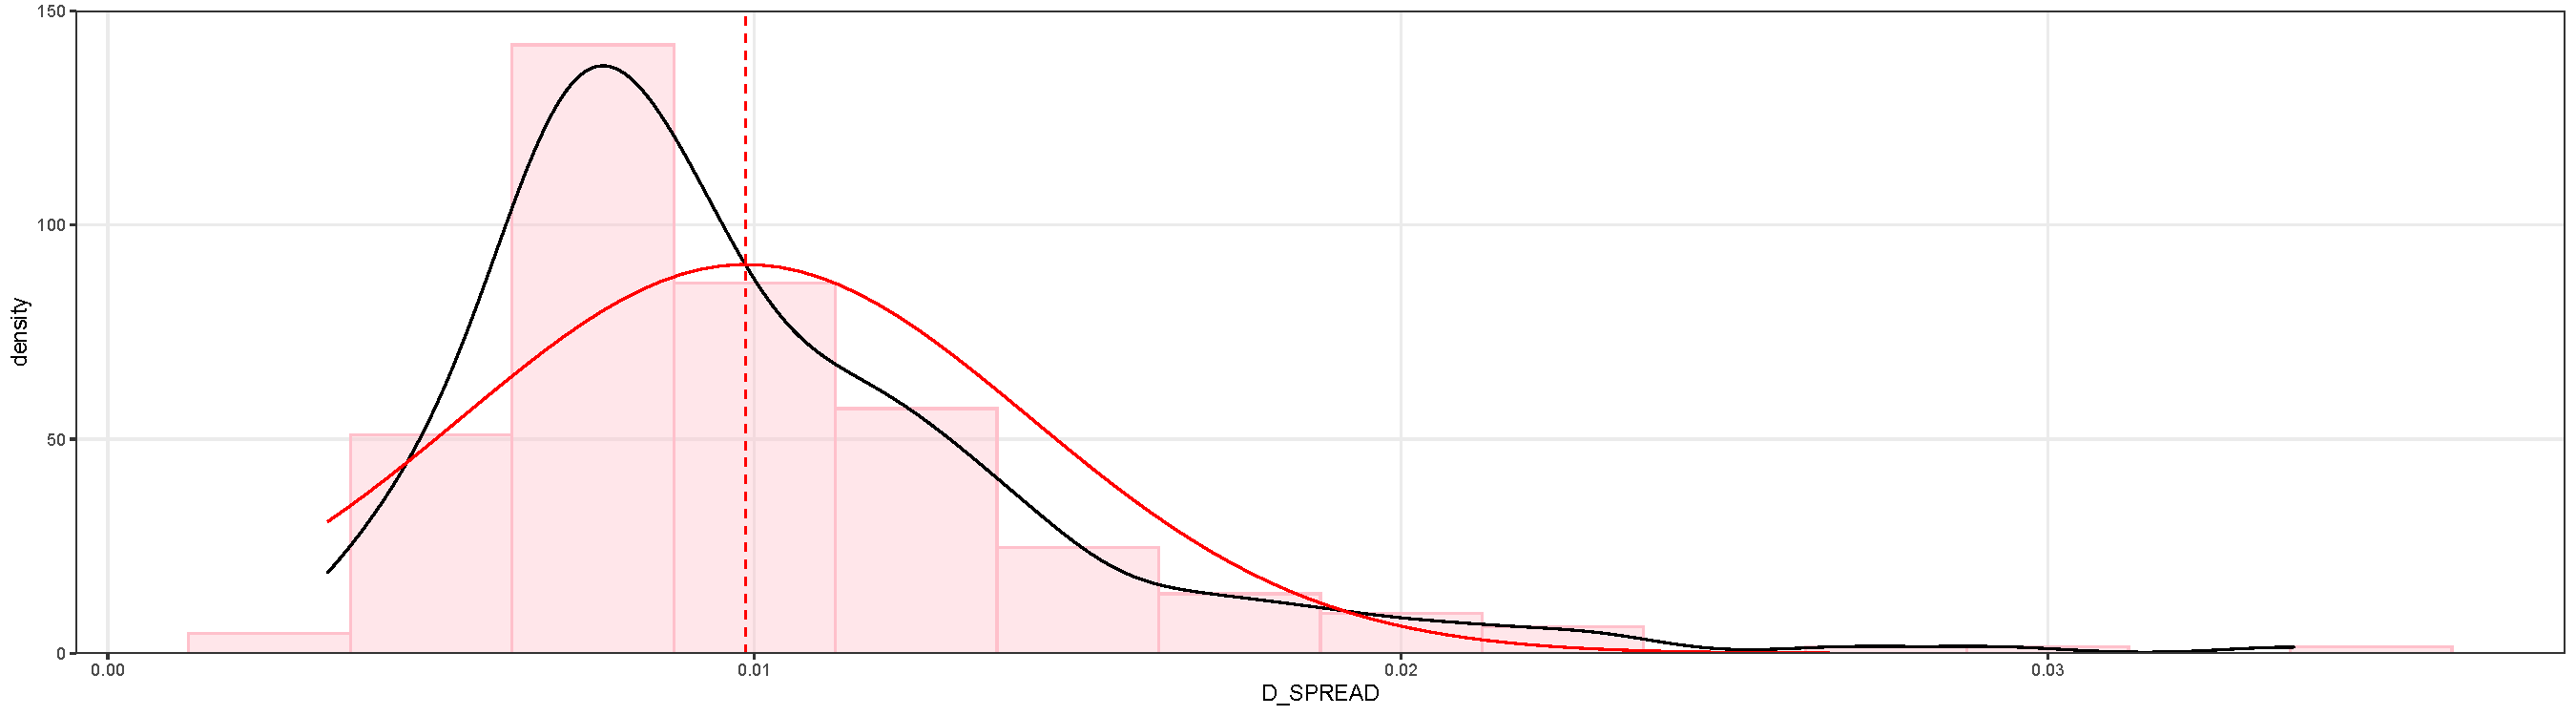
\includegraphics[width=1\linewidth]{Master_Thesis_Andreas_Kracht_Frandsen_files/figure-latex/DS-HIST-1} 

}

\caption{Autokorrelation af log netto renten.}\label{fig:DS-HIST}
\end{figure}

\hypertarget{federal-funds-rate-x_ttextfr}{%
\subsection{\texorpdfstring{Federal Funds Rate -- \(x_t^{\text{fr}}\)}{Federal Funds Rate -- x\_t\^{}\{\textbackslash text\{fr\}\}}}\label{federal-funds-rate-x_ttextfr}}

I U.S.A. er \emph{Federal Funds Rate}, renten som private finansinstitutioner tager for at låne uden sikkerhed, sædvanligvis over natten, af finansinstitutions reserver i \emph{Federal Reserve Bank}. Data er hentet fra \citep{FREDF2020}. De kvartalsvis observationer er baseret på et gennemsnit af daglige observationer. Middelværdien er på 4.814\(\%\), og standardafvigelsen er på 3.606\(\%\). Tredje og fjerde moment estimeres til hhv. 1.053 og 4.625. Figur \ref{fig:FR-tids} viser et plot over tidsserien.

\begin{figure}[htbp!]

{\centering 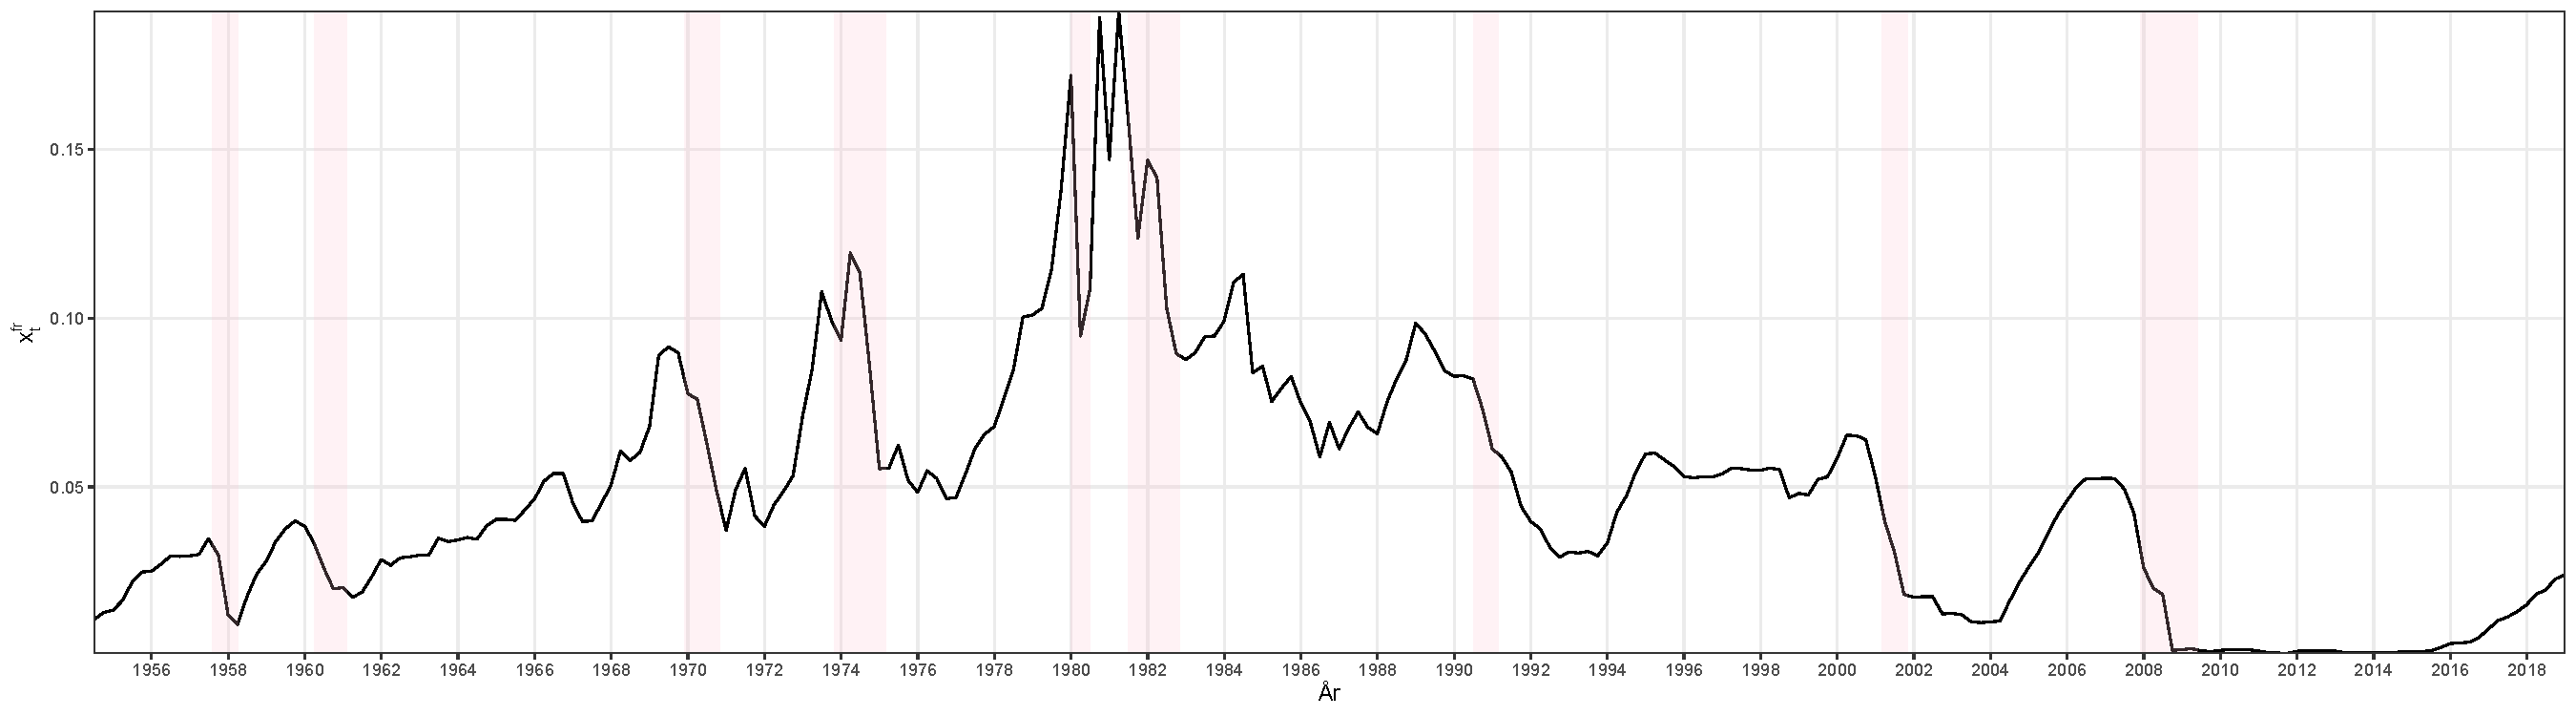
\includegraphics[width=1\linewidth]{Master_Thesis_Andreas_Kracht_Frandsen_files/figure-latex/FR-tids-1} 

}

\caption{Tidsserie af Federal Funds Rate.}\label{fig:FR-tids}
\end{figure}

\begin{figure}[htbp!]

{\centering 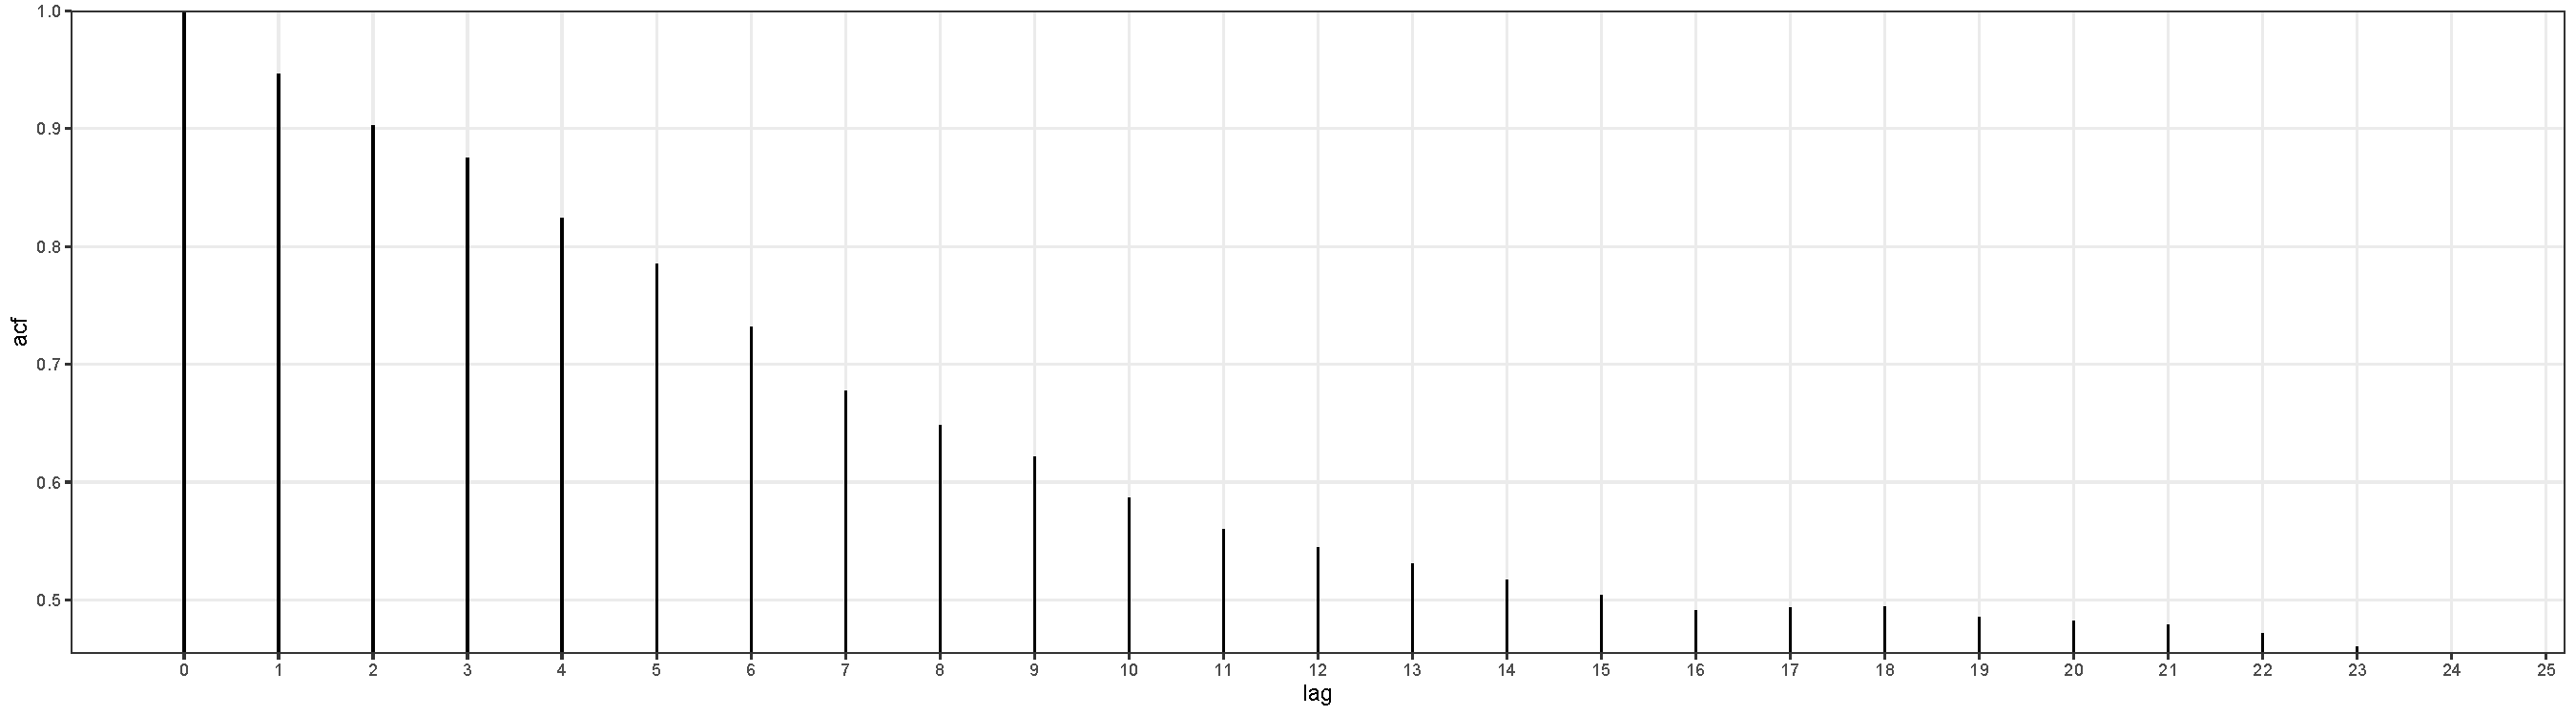
\includegraphics[width=1\linewidth]{Master_Thesis_Andreas_Kracht_Frandsen_files/figure-latex/FR-AK-1} 

}

\caption{Autokorrelation af log merafkastet af virksomhedsobligationer.}\label{fig:FR-AK}
\end{figure}

\begin{figure}[htbp!]

{\centering 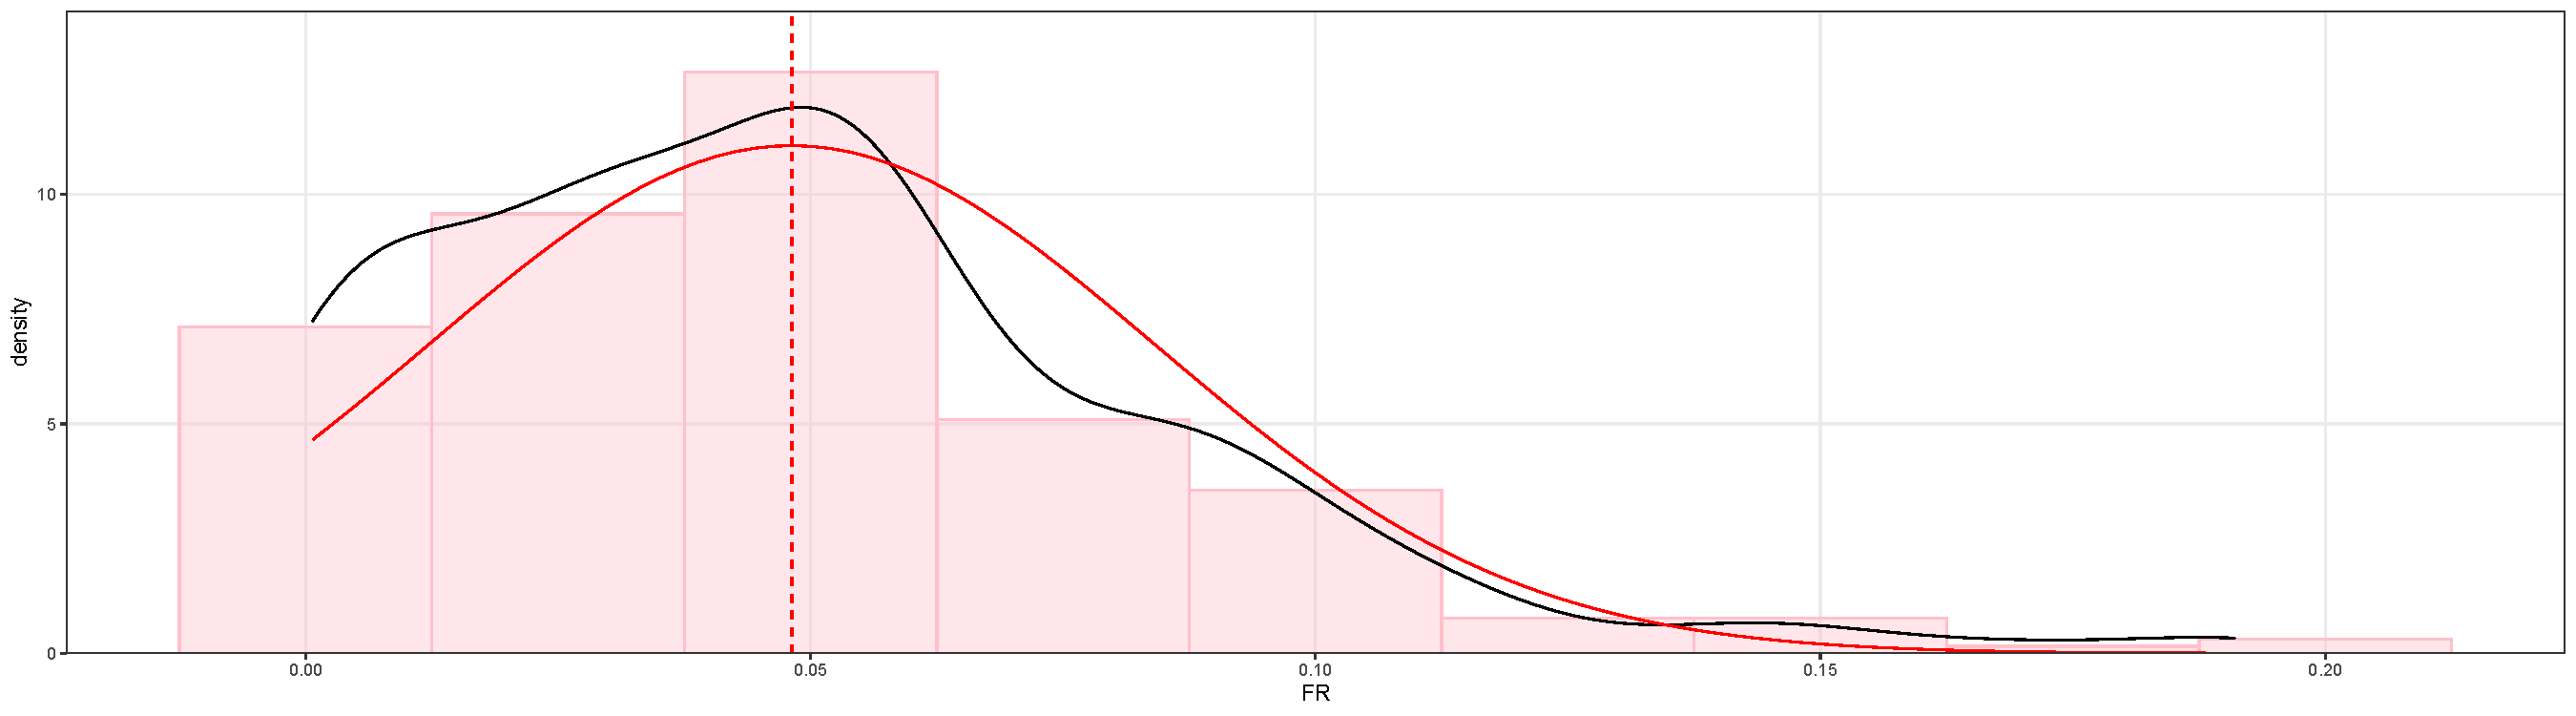
\includegraphics[width=1\linewidth]{Master_Thesis_Andreas_Kracht_Frandsen_files/figure-latex/FR-HIST-1} 

}

\caption{Autokorrelation af log netto renten.}\label{fig:FR-HIST}
\end{figure}

\begin{landscape}
\begin{table}[!h]

\caption{\label{tab:DES-TILSTANDSVARIABLE}Beskrivende statistik for prædiktionsvariablene.}
\centering
\begin{threeparttable}
\begin{tabular}[t]{lrrrrrrrrrr}
\toprule
  & Middelværdi & Standard afvigelse & Skævhed & Kurtosis & Minimum & $25 \%$ & Median & $75 \%$ & Maksimum & AK(1)\\
\midrule
\rowcolor{gray!6}  $x_t^{\text{dp}}$ & -3.516 & 0.371 & -0.371 & 2.370 & -4.489 & -3.889 & -3.531 & -3.292 & -2.894 & 0.972\\
$x_t^{\text{pe}}$ & 2.754 & 0.407 & 0.958 & 7.520 & 1.716 & 2.421 & 2.704 & 2.882 & 4.697 & 0.934\\
\rowcolor{gray!6}  $x_t^{\text{bm}}$ & 0.505 & 0.248 & 0.771 & 2.981 & 0.125 & 0.314 & 0.483 & 0.645 & 1.202 & 0.977\\
$x_t^{\text{avar}}$ & 0.006 & 0.010 & 7.186 & 68.380 & 0.000 & 0.002 & 0.004 & 0.007 & 0.108 & 0.423\\
\rowcolor{gray!6}  $x_t^{\text{hml}}$ & 0.330 & 1.809 & 0.447 & 4.858 & -6.043 & -0.837 & 0.300 & 1.138 & 8.093 & 0.114\\
$x_t^{\text{smb}}$ & 0.168 & 1.717 & 0.125 & 3.025 & -4.407 & -0.812 & 0.073 & 1.200 & 4.973 & 0.003\\
\rowcolor{gray!6}  $x_t^{\text{b}}$ & 0.012 & 0.008 & 0.903 & 4.313 & 0.000 & 0.006 & 0.011 & 0.016 & 0.042 & 0.922\\
$x_t^{\text{ts}}$ & 0.015 & 0.012 & -0.231 & 3.033 & -0.027 & 0.006 & 0.014 & 0.024 & 0.044 & 0.813\\
\rowcolor{gray!6}  $x_t^{\text{ys}}$ & 0.012 & 0.009 & -0.153 & 3.828 & -0.022 & 0.005 & 0.012 & 0.017 & 0.043 & 0.760\\
$x_t^{\text{cs}}$ & 0.034 & 0.017 & 0.159 & 2.330 & -0.008 & 0.020 & 0.033 & 0.048 & 0.084 & 0.887\\
\rowcolor{gray!6}  $x_t^{\text{ds}}$ & 0.010 & 0.004 & 1.842 & 8.156 & 0.003 & 0.007 & 0.009 & 0.012 & 0.034 & 0.870\\
$x_t^{\text{fr}}$ & 0.048 & 0.036 & 1.053 & 4.625 & 0.001 & 0.021 & 0.045 & 0.065 & 0.191 & 0.946\\
\bottomrule
\end{tabular}
\begin{tablenotes}
\item \textit{Note: } 
\item \textit{Denne tabel rapporterer kvartalsvis beskrivende statistik for prædiktionsvariablene: log Dividend-Price Ratio, log Price-Earnings Ratio, Book-to-Market Ratio, aktievariansen, High Minus Low, Small Minus Big, log afkastet af den nominelle rente, Term Spread, Yield Spread, Credit Spread, Default Spread samt Federal Funds Rate. Dette gøres ud fra $259$ kvartalvise observationer, som spænder over kvartalerne fra 2. kvartal 1954 til 4. kvartal 2018. Middelværdien er justeret for log Dividend-Price ratio, log Earnings-Price Ratio samt log afkastet af den nominelle rente.}
\end{tablenotes}
\end{threeparttable}
\end{table}

\begin{table}[!h]

\caption{\label{tab:JB-TILSTANDSVARIABLE}Jarque-Bera test.}
\centering
\begin{threeparttable}
\begin{tabular}[t]{lrr}
\toprule
  & Teststørrelse & $p$-værdi\\
\midrule
\rowcolor{gray!6}  $x_t^{\text{dp}}$ & 10.204 & 0.006\\
$x_t^{\text{pe}}$ & 260.174 & 0.000\\
\rowcolor{gray!6}  $x_t^{\text{bm}}$ & 25.633 & 0.000\\
$x_t^{\text{avar}}$ & 48357.914 & 0.000\\
\rowcolor{gray!6}  $x_t^{\text{hml}}$ & 45.881 & 0.000\\
$x_t^{\text{smb}}$ & 0.679 & 0.712\\
\rowcolor{gray!6}  $x_t^{\text{b}}$ & 53.814 & 0.000\\
$x_t^{\text{ts}}$ & 2.321 & 0.313\\
\rowcolor{gray!6}  $x_t^{\text{ys}}$ & 8.408 & 0.015\\
$x_t^{\text{cs}}$ & 5.942 & 0.051\\
\rowcolor{gray!6}  $x_t^{\text{ds}}$ & 433.398 & 0.000\\
$x_t^{\text{fr}}$ & 76.362 & 0.000\\
\bottomrule
\end{tabular}
\begin{tablenotes}
\item \textit{Note: } 
\item \textit{Denne tabel rapporterer Jarque-Beta teststørrelser og $p$-værdier for prædiktionsvariablene: log Dividend-Price Ratio, log Price-Earnings Ratio, Book-to-Market Ratio, aktievariansen, High Minus Low, Small Minus Big, log afkastet af den nominelle rente, Term Spread, Yield Spread, Credit Spread, Default Spread samt Federal Funds Rate, \citep{Jarque1980}. Dette gøres ud fra $259$ kvartalvise observationer, som spænder over kvartalerne fra 2. kvartal 1954 til 4. kvartal 2018.}
\end{tablenotes}
\end{threeparttable}
\end{table}
\end{landscape}

\hypertarget{korr}{%
\section{Korrelation}\label{korr}}

\begin{landscape}
\begin{table}[!h]

\caption{\label{tab:DES-KOR}Korrelationsmatricen mellem alle aktivklasser og prædiktionsvariable.}
\centering
\begin{threeparttable}
\begin{tabular}[t]{lrrrrrrrrrrrrrrrr}
\toprule
  & $r_t^{\text{rf}}$ & $rx_t^{\text{a}}$ & $rx_t^{\text{s}}$ & $rx_t^{\text{v}}$ & $x_t^{\text{dp}}$ & $x_t^{\text{pe}}$ & $x_t^{\text{bm}}$ & $x_t^{\text{avar}}$ & $x_t^{\text{hml}}$ & $x_t^{\text{smb}}$ & $x_t^{\text{b}}$ & $x_t^{\text{ts}}$ & $x_t^{\text{ys}}$ & $x_t^{\text{cs}}$ & $x_t^{\text{ds}}$ & $x_t^{\text{fr}}$\\
\midrule
\rowcolor{gray!6}  $r_t^{\text{rf}}$ & 1.00 & 0.00 & 0.32 & 0.34 & 0.14 & -0.06 & 0.06 & 0.21 & 0.02 & -0.07 & 0.43 & 0.01 & 0.11 & 0.01 & 0.20 & 0.29\\
$rx_t^{\text{a}}$ &  & 1.00 & -0.02 & 0.16 & -0.09 & 0.09 & -0.10 & -0.45 & -0.26 & 0.41 & -0.13 & 0.07 & 0.07 & -0.04 & -0.22 & -0.11\\
\rowcolor{gray!6}  $rx_t^{\text{s}}$ &  &  & 1.00 & 0.85 & -0.05 & 0.06 & -0.07 & 0.26 & -0.01 & -0.10 & 0.03 & 0.19 & 0.13 & 0.26 & 0.12 & -0.18\\
$rx_t^{\text{v}}$ &  &  &  & 1.00 & -0.09 & 0.14 & -0.11 & 0.24 & -0.01 & -0.05 & -0.05 & 0.24 & 0.18 & 0.26 & 0.04 & -0.23\\
\rowcolor{gray!6}  $x_t^{\text{dp}}$ &  &  &  &  & 1.00 & -0.71 & 0.88 & -0.06 & 0.04 & 0.00 & 0.50 & -0.09 & 0.03 & -0.21 & 0.28 & 0.48\\
$x_t^{\text{pe}}$ &  &  &  &  &  & 1.00 & -0.77 & 0.27 & -0.09 & 0.04 & -0.56 & 0.29 & 0.19 & 0.35 & -0.15 & -0.57\\
\rowcolor{gray!6}  $x_t^{\text{bm}}$ &  &  &  &  &  &  & 1.00 & -0.08 & 0.08 & 0.06 & 0.61 & -0.13 & -0.01 & -0.17 & 0.40 & 0.61\\
$x_t^{\text{avar}}$ &  &  &  &  &  &  &  & 1.00 & -0.09 & -0.13 & -0.04 & 0.16 & 0.10 & 0.35 & 0.42 & -0.09\\
\rowcolor{gray!6}  $x_t^{\text{hml}}$ &  &  &  &  &  &  &  &  & 1.00 & -0.10 & 0.09 & 0.06 & 0.07 & 0.02 & -0.03 & 0.06\\
$x_t^{\text{smb}}$ &  &  &  &  &  &  &  &  &  & 1.00 & -0.03 & 0.07 & 0.10 & 0.05 & 0.01 & 0.01\\
\rowcolor{gray!6}  $x_t^{\text{b}}$ &  &  &  &  &  &  &  &  &  &  & 1.00 & -0.20 & -0.03 & -0.16 & 0.42 & 0.90\\
$x_t^{\text{ts}}$ &  &  &  &  &  &  &  &  &  &  &  & 1.00 & 0.96 & 0.90 & 0.27 & -0.41\\
\rowcolor{gray!6}  $x_t^{\text{ys}}$ &  &  &  &  &  &  &  &  &  &  &  &  & 1.00 & 0.81 & 0.27 & -0.25\\
$x_t^{\text{cs}}$ &  &  &  &  &  &  &  &  &  &  &  &  &  & 1.00 & 0.53 & -0.36\\
\rowcolor{gray!6}  $x_t^{\text{ds}}$ &  &  &  &  &  &  &  &  &  &  &  &  &  &  & 1.00 & 0.32\\
$x_t^{\text{fr}}$ &  &  &  &  &  &  &  &  &  &  &  &  &  &  &  & 1.00\\
\bottomrule
\end{tabular}
\begin{tablenotes}
\item \textit{Note: } 
\item \textit{Denne tabel rapporterer den øvre triangulære korrelationsmatrix mellem alle beskrevne variable: det risikofrie aktiv, merafkastet på aktier, merafkastet på statsobligationer, merafkastet på virksomhedsobligationer, log Dividend-Price Ratio, log Price-Earnings Ratio, Book-to-Market Ratio, aktievariansen, High Minus Low, Small Minus Big, log afkastet af den nominelle rente, Term Spread, Yield Spread, Credit Spread, Default Spread samt Federal Funds Rate. Dette gøres ud fra $259$ kvartalvise observationer, som spænder over kvartalerne fra 2. kvartal 1954 til 4. kvartal 2018.}
\end{tablenotes}
\end{threeparttable}
\end{table}
\end{landscape}

\hypertarget{ops}{%
\section{Opsummering}\label{ops}}

\hypertarget{pruxe6diktabilitet}{%
\chapter{Prædiktabilitet}\label{pruxe6diktabilitet}}

\hypertarget{stationaritet}{%
\section{Stationaritet}\label{stationaritet}}






\begin{landscape}
\begin{table}[!h]

\caption{\label{tab:STAT}Augmented Dickey Fuller.}
\centering
\begin{threeparttable}
\begin{tabular}[t]{lrrrrrrrrrr}
\toprule
\multicolumn{1}{c}{ } & \multicolumn{2}{c}{$\delta=1$} & \multicolumn{2}{c}{$\delta=2$} & \multicolumn{2}{c}{$\delta=3$} & \multicolumn{2}{c}{$\delta=4$} & \multicolumn{2}{c}{$\delta=5$} \\
\cmidrule(l{3pt}r{3pt}){2-3} \cmidrule(l{3pt}r{3pt}){4-5} \cmidrule(l{3pt}r{3pt}){6-7} \cmidrule(l{3pt}r{3pt}){8-9} \cmidrule(l{3pt}r{3pt}){10-11}
  & Teststørrelse & $p$-værdi & Teststørrelse & $p$-værdi & Teststørrelse & $p$-værdi & Teststørrelse & $p$-værdi & Teststørrelse & $p$-værdi\\
\midrule
\rowcolor{gray!6}  $r_t^{\text{rf}}$ & -8.085 & 0.010 & -5.597 & 0.010 & -3.219 & 0.085 & -3.031 & 0.142 & -3.087 & 0.118\\
$rx_t^{\text{a}}$ & -11.556 & 0.010 & -9.732 & 0.010 & -8.465 & 0.010 & -7.542 & 0.010 & -7.115 & 0.010\\
\rowcolor{gray!6}  $rx_t^{\text{s}}$ & -12.079 & 0.010 & -8.889 & 0.010 & -7.598 & 0.010 & -8.364 & 0.010 & -7.580 & 0.010\\
$rx_t^{\text{v}}$ & -11.531 & 0.010 & -8.553 & 0.010 & -7.471 & 0.010 & -7.307 & 0.010 & -6.846 & 0.010\\
\rowcolor{gray!6}  $x_t^{\text{dp}}$ & -2.446 & 0.388 & -2.241 & 0.474 & -2.123 & 0.524 & -2.090 & 0.538 & -2.055 & 0.553\\
$x_t^{\text{pe}}$ & -4.675 & 0.010 & -4.545 & 0.010 & -3.620 & 0.032 & -3.189 & 0.090 & -3.555 & 0.038\\
\rowcolor{gray!6}  $x_t^{\text{bm}}$ & -2.220 & 0.483 & -2.173 & 0.503 & -2.046 & 0.557 & -2.073 & 0.545 & -1.896 & 0.620\\
$x_t^{\text{avar}}$ & -8.685 & 0.010 & -7.350 & 0.010 & -6.670 & 0.010 & -5.898 & 0.010 & -5.490 & 0.010\\
\rowcolor{gray!6}  $x_t^{\text{hml}}$ & -10.675 & 0.010 & -9.137 & 0.010 & -7.820 & 0.010 & -7.655 & 0.010 & -6.568 & 0.010\\
$x_t^{\text{smb}}$ & -10.072 & 0.010 & -8.590 & 0.010 & -6.413 & 0.010 & -6.087 & 0.010 & -5.751 & 0.010\\
\rowcolor{gray!6}  $x_t^{\text{b}}$ & -2.741 & 0.264 & -2.350 & 0.429 & -2.517 & 0.358 & -2.687 & 0.287 & -2.773 & 0.250\\
$x_t^{\text{ts}}$ & -4.946 & 0.010 & -4.022 & 0.010 & -5.036 & 0.010 & -4.502 & 0.010 & -5.266 & 0.010\\
\rowcolor{gray!6}  $x_t^{\text{ys}}$ & -5.449 & 0.010 & -4.319 & 0.010 & -5.076 & 0.010 & -4.749 & 0.010 & -5.284 & 0.010\\
$x_t^{\text{cs}}$ & -4.490 & 0.010 & -3.856 & 0.017 & -5.020 & 0.010 & -4.670 & 0.010 & -5.265 & 0.010\\
\rowcolor{gray!6}  $x_t^{\text{ds}}$ & -4.622 & 0.010 & -4.142 & 0.010 & -4.042 & 0.010 & -3.983 & 0.010 & -3.511 & 0.042\\
$x_t^{\text{fr}}$ & -2.734 & 0.267 & -2.408 & 0.404 & -2.844 & 0.221 & -2.592 & 0.327 & -3.131 & 0.100\\
\bottomrule
\end{tabular}
\begin{tablenotes}
\item \textit{Note: } 
\item \textit{Denne tabel rapporterer Augmented Dickey Fuller teststørrelser og $p$-værdier for alle beskrevne variable: det risikofrie aktiv, merafkastet på aktier, merafkastet på statsobligationer, merafkastet på virksomhedsobligationer, log Dividend-Price Ratio, log Price-Earnings Ratio, Book-to-Market Ratio, aktievariansen, High Minus Low, Small Minus Big, log afkastet af den nominelle rente, Term Spread, Yield Spread, Credit Spread, Default Spread samt Federal Funds Rate, \citep{Dickey1979}. Testen er udført for forskellige lags, samt et lag fastsat til heltalsdelen af $4(T/100)^{1/4}$ -- som foreslået af \citep{Schwert1989} -- hvor $T=259$. Dette gøres ud fra $259$ kvartalvise observationer, som spænder over kvartalerne fra 2. kvartal 1954 til 4. kvartal 2018.}
\end{tablenotes}
\end{threeparttable}
\end{table}
\end{landscape}

\begin{table}[!h]

\caption{\label{tab:STAT-KPSS}Kwiatkowski-Phillips-Schmidt-Shin Test.}
\centering
\begin{threeparttable}
\begin{tabular}[t]{lrrrr}
\toprule
\multicolumn{1}{c}{ } & \multicolumn{4}{c}{$l=5$} \\
\cmidrule(l{3pt}r{3pt}){2-5}
\multicolumn{1}{c}{ } & \multicolumn{2}{c}{Level} & \multicolumn{2}{c}{Trend} \\
\cmidrule(l{3pt}r{3pt}){2-3} \cmidrule(l{3pt}r{3pt}){4-5}
  & Teststørrelse (LM) & $p$-værdi & Teststørrelse (LM) & $p$-værdi\\
\midrule
\rowcolor{gray!6}  $r_t^{\text{rf}}$ & 0.500 & 0.042 & 0.334 & 0.010\\
$rx_t^{\text{a}}$ & 0.059 & 0.100 & 0.060 & 0.100\\
\rowcolor{gray!6}  $rx_t^{\text{s}}$ & 0.469 & 0.049 & 0.039 & 0.100\\
$rx_t^{\text{v}}$ & 0.581 & 0.024 & 0.037 & 0.100\\
\rowcolor{gray!6}  $x_t^{\text{dp}}$ & 2.448 & 0.010 & 0.397 & 0.010\\
$x_t^{\text{pe}}$ & 1.526 & 0.010 & 0.326 & 0.010\\
\rowcolor{gray!6}  $x_t^{\text{bm}}$ & 2.102 & 0.010 & 0.501 & 0.010\\
$x_t^{\text{avar}}$ & 0.626 & 0.020 & 0.046 & 0.100\\
\rowcolor{gray!6}  $x_t^{\text{hml}}$ & 0.185 & 0.100 & 0.052 & 0.100\\
$x_t^{\text{smb}}$ & 0.063 & 0.100 & 0.051 & 0.100\\
\rowcolor{gray!6}  $x_t^{\text{b}}$ & 1.191 & 0.010 & 0.794 & 0.010\\
$x_t^{\text{ts}}$ & 0.753 & 0.010 & 0.071 & 0.100\\
\rowcolor{gray!6}  $x_t^{\text{ys}}$ & 0.331 & 0.100 & 0.132 & 0.075\\
$x_t^{\text{cs}}$ & 1.671 & 0.010 & 0.079 & 0.100\\
\rowcolor{gray!6}  $x_t^{\text{ds}}$ & 0.451 & 0.055 & 0.297 & 0.010\\
$x_t^{\text{fr}}$ & 1.155 & 0.010 & 0.754 & 0.010\\
\bottomrule
\end{tabular}
\begin{tablenotes}
\item \textit{Note: } 
\item \textit{Denne tabel rapporterer Kwiatkowski-Phillips-Schmidt-Shin teststørrelser og $p$-værdier for alle beskrevne variable: det risikofrie aktiv, merafkastet på aktier, merafkastet på statsobligationer, merafkastet på virksomhedsobligationer, log Dividend-Price Ratio, log Price-Earnings Ratio, Book-to-Market Ratio, aktievariansen, High Minus Low, Small Minus Big, log afkastet af den nominelle rente, Term Spread, Yield Spread, Credit Spread, Default Spread samt Federal Funds Rate, \citep{Kwiatkowski1992}. Dette gøres ud fra $259$ kvartalvise observationer, som spænder over kvartalerne fra 2. kvartal 1954 til 4. kvartal 2018. Testen er udført for et lag fastsat til heltalsdelen af $4(T/100)^{1/4}$ -- som foreslået af \citep{Schwert1989} -- hvor $T=259$.}
\end{tablenotes}
\end{threeparttable}
\end{table}

\begin{table}[!h]

\caption{\label{tab:STAT-PP}Phillips-Perron Test.}
\centering
\begin{threeparttable}
\begin{tabular}[t]{lrrrr}
\toprule
\multicolumn{1}{c}{ } & \multicolumn{4}{c}{$l=5$} \\
\cmidrule(l{3pt}r{3pt}){2-5}
\multicolumn{1}{c}{ } & \multicolumn{2}{c}{$Z(\hat{\alpha})$} & \multicolumn{2}{c}{$Z(t_{\hat{\alpha}})$} \\
\cmidrule(l{3pt}r{3pt}){2-3} \cmidrule(l{3pt}r{3pt}){4-5}
  & Teststørrelse & $p$-værdi & Teststørrelse & $p$-værdi\\
\midrule
\rowcolor{gray!6}  $r_t^{\text{rf}}$ & -233.688 & 0.010 & -12.546 & 0.010\\
$rx_t^{\text{a}}$ & -220.300 & 0.010 & -14.622 & 0.010\\
\rowcolor{gray!6}  $rx_t^{\text{s}}$ & -250.336 & 0.010 & -16.088 & 0.010\\
$rx_t^{\text{v}}$ & -285.340 & 0.010 & -17.145 & 0.010\\
\rowcolor{gray!6}  $x_t^{\text{dp}}$ & -10.744 & 0.507 & -2.301 & 0.449\\
$x_t^{\text{pe}}$ & -26.987 & 0.015 & -3.700 & 0.024\\
\rowcolor{gray!6}  $x_t^{\text{bm}}$ & -8.338 & 0.642 & -2.045 & 0.557\\
$x_t^{\text{avar}}$ & -157.735 & 0.010 & -10.522 & 0.010\\
\rowcolor{gray!6}  $x_t^{\text{hml}}$ & -223.350 & 0.010 & -14.277 & 0.010\\
$x_t^{\text{smb}}$ & -285.632 & 0.010 & -15.960 & 0.010\\
\rowcolor{gray!6}  $x_t^{\text{b}}$ & -16.685 & 0.174 & -3.088 & 0.118\\
$x_t^{\text{ts}}$ & -55.607 & 0.010 & -5.436 & 0.010\\
\rowcolor{gray!6}  $x_t^{\text{ys}}$ & -64.954 & 0.010 & -5.958 & 0.010\\
$x_t^{\text{cs}}$ & -45.693 & 0.010 & -4.839 & 0.010\\
\rowcolor{gray!6}  $x_t^{\text{ds}}$ & -35.018 & 0.010 & -4.317 & 0.010\\
$x_t^{\text{fr}}$ & -14.944 & 0.272 & -2.895 & 0.199\\
\bottomrule
\end{tabular}
\begin{tablenotes}
\item \textit{Note: } 
\item \textit{Denne tabel rapporterer Phillips-Perron teststørrelser og $p$-værdier for alle beskrevne variable: det risikofrie aktiv, merafkastet på aktier, merafkastet på statsobligationer, merafkastet på virksomhedsobligationer, log Dividend-Price Ratio, log Price-Earnings Ratio, Book-to-Market Ratio, aktievariansen, High Minus Low, Small Minus Big, log afkastet af den nominelle rente, Term Spread, Yield Spread, Credit Spread, Default Spread samt Federal Funds Rate, \citep{Phillips1988}. Dette gøres ud fra $259$ kvartalvise observationer, som spænder over kvartalerne fra 2. kvartal 1954 til 4. kvartal 2018. Testen er udført for et lag fastsat til heltalsdelen af $4(T/100)^{1/4}$ -- som foreslået af \citep{Schwert1989} -- hvor $T=259$.}
\end{tablenotes}
\end{threeparttable}
\end{table}

\hypertarget{univariat}{%
\section{Univariat}\label{univariat}}



\begin{table}[!h]

\caption{\label{tab:UNI-ak}Univariat prædiktabilitet af merafkastet på aktier.}
\centering
\begin{threeparttable}
\begin{tabular}[t]{lrrrrrrr}
\toprule
\multicolumn{1}{c}{ } & \multicolumn{1}{c}{ } & \multicolumn{2}{c}{Konfidensinterval} & \multicolumn{4}{c}{ } \\
\cmidrule(l{3pt}r{3pt}){3-4}
  & Koefficient & Nedre & Øvre & Standardfejl & $t$-værdi & $p$ & $R^2$\\
\midrule
\rowcolor{gray!6}  $x_t^{\text{dp}}$ & 0.024 & -0.005 & 0.054 & 0.015 & 1.606 & 0.110 & 0.011\\
$x_t^{\text{pe}}$ & -0.009 & -0.044 & 0.027 & 0.018 & -0.480 & 0.631 & 0.002\\
\rowcolor{gray!6}  $x_t^{\text{bm}}$ & 0.016 & -0.024 & 0.056 & 0.020 & 0.779 & 0.437 & 0.002\\
$x_t^{\sigma_{\text{a}}^2}$ & 0.278 & -1.317 & 1.873 & 0.810 & 0.343 & 0.732 & 0.001\\
\rowcolor{gray!6}  $x_t^{\text{hml}}$ & -0.004 & -0.009 & 0.001 & 0.003 & -1.496 & 0.136 & 0.007\\
$x_t^{\text{smb}}$ & \textbf{-0.006} & -0.010 & -0.002 & 0.002 & -2.671 & 0.008 & 0.015\\
\rowcolor{gray!6}  $x_t^{\text{b}}$ & -0.850 & -2.110 & 0.410 & 0.640 & -1.328 & 0.185 & 0.007\\
$x_t^{\text{ts}}$ & \textbf{ 0.976} & 0.083 & 1.870 & 0.454 & 2.152 & 0.032 & 0.019\\
\rowcolor{gray!6}  $x_t^{\text{ys}}$ & 1.014 & -0.035 & 2.062 & 0.532 & 1.904 & 0.058 & 0.013\\
$x_t^{\text{cs}}$ & 0.312 & -0.502 & 1.126 & 0.413 & 0.755 & 0.451 & 0.004\\
\rowcolor{gray!6}  $x_t^{\text{ds}}$ & -1.049 & -5.042 & 2.944 & 2.028 & -0.517 & 0.605 & 0.003\\
$x_t^{\text{fr}}$ & \textbf{-0.386} & -0.697 & -0.075 & 0.158 & -2.445 & 0.015 & 0.028\\
\bottomrule
\end{tabular}
\begin{tablenotes}
\item \textit{Note: } 
\item \textit{Denne tabel rapporterer den beskrivende statistik af de univariate regressioner ift. responsvariablen: merafkastet på aktier, $rx_{t+1}^{\text{a}}$. Hver række svarer til én selvstændig regression. Dette gøres ud fra $259$ kvartalvise observationer, som spænder over kvartalerne fra 2. kvartal 1954 til 4. kvartal 2018. Koefficienter markeret med \textbf{fed} implicerer signifikans, for et signifikansniveau på $\alpha=0.05$. Standardfejl er justeret for heteroskedasticitet og autokorrelation, \citep{Newey1987}. Konfidensintervallerne for koefficienterne, $t$-værdierne og $p$-værdierne er ligedes dannet på baggrund af de justerede standardfejl. $R^2$ er ligedes rapporteret, bemærk dette ikke er den justerede $R^2$.}
\end{tablenotes}
\end{threeparttable}
\end{table}

\begin{table}[!h]

\caption{\label{tab:UNI-s}Univariat prædiktabilitet af merafkastet på statsobligationer.}
\centering
\begin{threeparttable}
\begin{tabular}[t]{lrrrrrrr}
\toprule
\multicolumn{1}{c}{ } & \multicolumn{1}{c}{ } & \multicolumn{2}{c}{Konfidensinterval} & \multicolumn{4}{c}{ } \\
\cmidrule(l{3pt}r{3pt}){3-4}
  & Koefficient & Nedre & Øvre & Standardfejl & $t$-værdi & $p$ & $R^2$\\
\midrule
\rowcolor{gray!6}  $x_t^{\text{dp}}$ & -0.006 & -0.019 & 0.008 & 0.007 & -0.852 & 0.395 & 0.003\\
$x_t^{\text{pe}}$ & 0.001 & -0.010 & 0.013 & 0.006 & 0.196 & 0.845 & 0.000\\
\rowcolor{gray!6}  $x_t^{\text{bm}}$ & -0.007 & -0.030 & 0.017 & 0.012 & -0.545 & 0.586 & 0.002\\
$x_t^{\sigma_{\text{a}}^2}$ & 0.107 & -0.178 & 0.391 & 0.145 & 0.738 & 0.461 & 0.001\\
\rowcolor{gray!6}  $x_t^{\text{hml}}$ & 0.001 & -0.002 & 0.004 & 0.001 & 0.776 & 0.439 & 0.002\\
$x_t^{\text{smb}}$ & \textbf{-0.004} & -0.007 & -0.001 & 0.001 & -2.702 & 0.007 & 0.031\\
\rowcolor{gray!6}  $x_t^{\text{b}}$ & -0.012 & -0.864 & 0.840 & 0.433 & -0.028 & 0.978 & 0.000\\
$x_t^{\text{ts}}$ & \textbf{ 0.590} & 0.119 & 1.062 & 0.239 & 2.466 & 0.014 & 0.033\\
\rowcolor{gray!6}  $x_t^{\text{ys}}$ & 0.454 & -0.216 & 1.124 & 0.340 & 1.334 & 0.183 & 0.012\\
$x_t^{\text{cs}}$ & \textbf{ 0.632} & 0.342 & 0.921 & 0.147 & 4.297 & 0.000 & 0.081\\
\rowcolor{gray!6}  $x_t^{\text{ds}}$ & \textbf{ 1.885} & 0.586 & 3.184 & 0.660 & 2.858 & 0.005 & 0.047\\
$x_t^{\text{fr}}$ & -0.139 & -0.280 & 0.003 & 0.072 & -1.934 & 0.054 & 0.017\\
\bottomrule
\end{tabular}
\begin{tablenotes}
\item \textit{Note: } 
\item \textit{Denne tabel rapporterer den beskrivende statistik af de univariate regressioner ift. responsvariablen: merafkastet på statsobligationer, $rx_{t+1}^{\text{s}}$. Hver række svarer til én selvstændig regression. Dette gøres ud fra $259$ kvartalvise observationer, som spænder over kvartalerne fra 2. kvartal 1954 til 4. kvartal 2018. Koefficienter markeret med \textbf{fed} implicerer signifikans, for et signifikansniveau på $\alpha=0.05$. Standardfejl er justeret for heteroskedasticitet og autokorrelation, \citep{Newey1987}. Konfidensintervallerne for koefficienterne, $t$-værdierne og $p$-værdierne er ligedes dannet på baggrund af de justerede standardfejl. $R^2$ er ligedes rapporteret, bemærk dette ikke er den justerede $R^2$.}
\end{tablenotes}
\end{threeparttable}
\end{table}

\begin{table}[!h]

\caption{\label{tab:UNI-v}Univariat prædiktabilitet af merafkastet på virksomhedsobligationer}
\centering
\begin{threeparttable}
\begin{tabular}[t]{lrrrrrrr}
\toprule
\multicolumn{1}{c}{ } & \multicolumn{1}{c}{ } & \multicolumn{2}{c}{Konfidensinterval} & \multicolumn{4}{c}{ } \\
\cmidrule(l{3pt}r{3pt}){3-4}
  & Koefficient & Nedre & Øvre & Standardfejl & $t$-værdi & $p$ & $R^2$\\
\midrule
\rowcolor{gray!6}  $x_t^{\text{dp}}$ & -0.007 & -0.024 & 0.010 & 0.009 & -0.797 & 0.426 & 0.003\\
$x_t^{\text{pe}}$ & 0.009 & -0.007 & 0.025 & 0.008 & 1.084 & 0.279 & 0.006\\
\rowcolor{gray!6}  $x_t^{\text{bm}}$ & -0.010 & -0.041 & 0.021 & 0.016 & -0.660 & 0.510 & 0.003\\
$x_t^{\sigma_{\text{a}}^2}$ & 0.077 & -0.594 & 0.748 & 0.341 & 0.227 & 0.821 & 0.000\\
\rowcolor{gray!6}  $x_t^{\text{hml}}$ & 0.002 & -0.001 & 0.006 & 0.002 & 1.236 & 0.218 & 0.008\\
$x_t^{\text{smb}}$ & \textbf{-0.004} & -0.008 & -0.001 & 0.002 & -2.304 & 0.022 & 0.024\\
\rowcolor{gray!6}  $x_t^{\text{b}}$ & -0.447 & -1.542 & 0.647 & 0.556 & -0.805 & 0.422 & 0.006\\
$x_t^{\text{ts}}$ & \textbf{ 1.146} & 0.438 & 1.854 & 0.360 & 3.188 & 0.002 & 0.084\\
\rowcolor{gray!6}  $x_t^{\text{ys}}$ & \textbf{ 1.142} & 0.161 & 2.123 & 0.498 & 2.292 & 0.023 & 0.051\\
$x_t^{\text{cs}}$ & \textbf{ 0.958} & 0.585 & 1.330 & 0.189 & 5.063 & 0.000 & 0.125\\
\rowcolor{gray!6}  $x_t^{\text{ds}}$ & \textbf{ 2.369} & 0.892 & 3.847 & 0.750 & 3.158 & 0.002 & 0.049\\
$x_t^{\text{fr}}$ & \textbf{-0.282} & -0.484 & -0.079 & 0.103 & -2.739 & 0.007 & 0.047\\
\bottomrule
\end{tabular}
\begin{tablenotes}
\item \textit{Note: } 
\item \textit{Denne tabel rapporterer den beskrivende statistik af de univariate regressioner ift. responsvariablen: merafkastet på virksomhedsobligationer, $rx_{t+1}^{\text{v}}$. Hver række svarer til én selvstændig regression. Dette gøres ud fra $259$ kvartalvise observationer, som spænder over kvartalerne fra 2. kvartal 1954 til 4. kvartal 2018. Koefficienter markeret med \textbf{fed} implicerer signifikans, for et signifikansniveau på $\alpha=0.05$. Standardfejl er justeret for heteroskedasticitet og autokorrelation, \citep{Newey1987}. Konfidensintervallerne for koefficienterne, $t$-værdierne og $p$-værdierne er ligedes dannet på baggrund af de justerede standardfejl. $R^2$ er ligedes rapporteret, bemærk dette ikke er den justerede $R^2$.}
\end{tablenotes}
\end{threeparttable}
\end{table}

\hypertarget{underliggende-model}{%
\chapter{Underliggende model}\label{underliggende-model}}

\hypertarget{problemer-ved-estimation}{%
\chapter{Problemer ved estimation}\label{problemer-ved-estimation}}

Middelværdi-varians optimering har vist sig meget sensitiv overfor den kvantitative størrelse af parametrene som indgår i vægtelsesberegningen for den relevante portefølje, dvs. forventede afkast, varianser og kovarianser. Som også er tilfældet i denne afhandling, er disse parametre estimeret via en tidsserie af afkast, men forventningen til disse estimater skal anskues skeptisk, idet de indeholder en væsentlig mængde usikkerhed.

Simuleringsforsøg har vist at porteføljer udvalgt på baggrund af Markowitz teorien med estimerede input har værre performance og er mindre efficiente end en \(\tfrac{1}{n}\) (ligevægtet) portefølje, \citep{Frankfurter1971}. Ligeledes viser \citep{Chopra1993}, at det er afgørende i en porteføljeanalyse at estimere forventede afkast præcist, men forventede afkast er alt andet lige svært prædiktable, \citep{Merton1980}. Videnskabelige artikler har foreslået ændringer til de statistiske metoder som ligger bag estimaterne, heriblandt foreslår \citep{Jorion1986} at benytte en Bayes-estimator i stedet for det aritmetiske gennemsnit, se evt. også \citep{MacKinlay2000}, \citep{Garlappi2007}, \citep{Kan2007}, \citep{Tu2011}.

I det følgende, vil et illustrativt \emph{Monte Carlo} simuleringseksempel blive foretaget, hvor der tages udgangspunkt i tre risikobærende aktiver, hvis kvartalvise afkast alle er normalfordelt med de første to momenter som set i Tabel \ref{tab:true}. Afkastene er identisk fordelte i alle kvartaler. Det årlige forventede afkast er hhv. \(9\%\), \(15.76\%\) og \(5.12\%\). Standardafvigelsen er hhv. \(20.694\%\), \(25.794\%\) og \(17.320\%\). Det antages, at der er ens positiv korrelation mellem hvert aktiv, på \(0.5\). Derudover står investoren overfor et risikofrit aktiv med et kvartalvist afkast på \(0.125\%\), og dermed et årligt risikofrit afkast på \(0.5\%\). Disse er de sande parameterværdier, som givetvis er skjult information for investoren til en hvis grad. Investoren skal dermed estimere værdierne fra en tidsserie af observationer trukket fra den korrekte fordeling. Tre tidsserier af afkastsobservationer er blevet simuleret fra den relevante multivariate fordeling. Hver observation er hhv. beregnet som
\begin{align*}
r_1 &= \mu_1 + \sigma_1\nu_1\\
r_2 &= \mu_2 + \sigma_2\left(\rho_{1,2}\nu_1 + \sqrt{1-\rho_{1,2}^2}\nu_2\right)\\
r_3 &= \mu_3 + \sigma_3 \left( \rho_{1,3} \nu_1+ \frac{ \rho_{2,3}-\rho_{1,2}\rho_{1,3} }{\sqrt{1-\rho_{1,2}^2}}\nu_2+\sqrt{1-\rho_{1,3}^2 -\frac{\left(\rho_{2,3}-\rho_{1,2}\rho_{1,3}\right)^2}{1-\rho_{1,2}^2}}\nu_3\right),
\end{align*}

hvor \(\mu_i\) er middelværdien, \(\sigma_i\) er standardafvigelsen og \(\nu_i\sim N(0,1)\) er stød til tidsserien, for \(i=1,2,3\).

\begin{figure}[htbp!]

{\centering \includegraphics[width=1\linewidth]{Master_Thesis_Andreas_Kracht_Frandsen_files/figure-latex/sim-tids-1} 

}

\caption{Simulerede afkast fra første simulering.}\label{fig:sim-tids}
\end{figure}

Hver tidsserie er baseret på \(200\) observationer, svarende til en 50-årig periode med kvartalvise observationer. For hver tidsserie er de første to momenter estimeret ud fra de gængse statistiske metoder

\begin{table}[!h]

\caption{\label{tab:true}Gengivelse af de sande afkast.}
\centering
\begin{tabular}[t]{lrrrrr}
\toprule
\multicolumn{1}{c}{ } & \multicolumn{1}{c}{Forventet afkast} & \multicolumn{1}{c}{Volatilitet} & \multicolumn{3}{c}{Korrelationer} \\
\cmidrule(l{3pt}r{3pt}){2-2} \cmidrule(l{3pt}r{3pt}){3-3} \cmidrule(l{3pt}r{3pt}){4-6}
\rowcolor{gray!6}  Aktiv 1 & 2.25 & 10.347 & 1.0 & 0.5 & 0.5\\
Aktiv 2 & 3.94 & 12.899 & 0.5 & 1.0 & 0.5\\
\rowcolor{gray!6}  Aktiv 3 & 1.28 & 8.660 & 0.5 & 0.5 & 1.0\\
\bottomrule
\end{tabular}
\end{table}

\begin{table}[!h]

\caption{\label{tab:sim1}Gengivelse af første simulation af afkast.}
\centering
\begin{tabular}[t]{lrrrrrr}
\toprule
\multicolumn{1}{c}{ } & \multicolumn{1}{c}{Forventet afkast} & \multicolumn{1}{c}{Volatilitet} & \multicolumn{1}{c}{Relativ fejl} & \multicolumn{3}{c}{Korrelationer} \\
\cmidrule(l{3pt}r{3pt}){2-2} \cmidrule(l{3pt}r{3pt}){3-3} \cmidrule(l{3pt}r{3pt}){4-4} \cmidrule(l{3pt}r{3pt}){5-7}
\rowcolor{gray!6}  Aktiv 1 & 2.741 & 10.835 & 0.548 & 1.000 & 0.524 & 0.487\\
Aktiv 2 & 4.931 & 12.640 & 0.355 & 0.524 & 1.000 & 0.488\\
\rowcolor{gray!6}  Aktiv 3 & 1.112 & 8.503 & 1.059 & 0.487 & 0.488 & 1.000\\
\bottomrule
\end{tabular}
\end{table}

\begin{table}[!h]

\caption{\label{tab:sim2}Gengivelse af anden simulation af afkast.}
\centering
\begin{tabular}[t]{lrrrrrr}
\toprule
\multicolumn{1}{c}{ } & \multicolumn{1}{c}{Forventet afkast} & \multicolumn{1}{c}{Volatilitet} & \multicolumn{1}{c}{Relativ fejl} & \multicolumn{3}{c}{Korrelationer} \\
\cmidrule(l{3pt}r{3pt}){2-2} \cmidrule(l{3pt}r{3pt}){3-3} \cmidrule(l{3pt}r{3pt}){4-4} \cmidrule(l{3pt}r{3pt}){5-7}
\rowcolor{gray!6}  Aktiv 1 & 0.930 & 11.194 & 1.668 & 1.000 & 0.489 & 0.459\\
Aktiv 2 & 2.200 & 12.442 & 0.784 & 0.489 & 1.000 & 0.453\\
\rowcolor{gray!6}  Aktiv 3 & 0.777 & 9.198 & 1.641 & 0.459 & 0.453 & 1.000\\
\bottomrule
\end{tabular}
\end{table}

\begin{table}[!h]

\caption{\label{tab:sim3}Gengivelse af tredje simulation af afkast.}
\centering
\begin{tabular}[t]{lrrrrrr}
\toprule
\multicolumn{1}{c}{ } & \multicolumn{1}{c}{Forventet afkast} & \multicolumn{1}{c}{Volatilitet} & \multicolumn{1}{c}{Relativ fejl} & \multicolumn{3}{c}{Korrelationer} \\
\cmidrule(l{3pt}r{3pt}){2-2} \cmidrule(l{3pt}r{3pt}){3-3} \cmidrule(l{3pt}r{3pt}){4-4} \cmidrule(l{3pt}r{3pt}){5-7}
\rowcolor{gray!6}  Aktiv 1 & 2.793 & 10.056 & 0.499 & 1.000 & 0.479 & 0.483\\
Aktiv 2 & 4.374 & 13.878 & 0.440 & 0.479 & 1.000 & 0.519\\
\rowcolor{gray!6}  Aktiv 3 & 0.901 & 9.266 & 1.426 & 0.483 & 0.519 & 1.000\\
\bottomrule
\end{tabular}
\end{table}

Disse tre sæt af estimerede parametre, baseret på de tre tidsserier, er blevet udvalgt til det følgende illustrative formål. Se Tabel \ref{tab:sim1}, Tabel \ref{tab:sim2} og Tabel \ref{tab:sim3} for en sammenligning ift. de sande parametre. De relative fejl for hver simulering er ligedes rapporteret, \citep{Asmussen2007}. Disse beregnes som
\[\varepsilon_{i,j} = \frac{z_{0.975}\hat{\sigma}_{i,j}}{\sqrt{R}\hat{\mu}_{i,j}},\]

hvor \(i=1,2,3\) repræsenterer aktiverne og \(j=1,2,3\) repræsenterer simuleringen. \(z_{0.975}\) er fraktilfunktionen fra standard normal fordelingen, for et signifikansniveau på \(\alpha=0.05\). \(R\) er antallet af observationer fra hver simulering, i dette forsøg er \(R=200\).

Ud fra de sande parametre samt de estimerede parametre fra de tre tidsserier er global minimum varians porteføljen, tangensporteføljen, den optimale portefølje for en \emph{CRRA} investor med risikoaversions parameter lig hhv. \(1\), \(5\) og \(10\), samt den optimale portefølje for en \emph{CARA} investor med risikoaversions parameter lig hhv. \(1\), \(5\) og \(10\).

Porteføljen for \emph{CARA}-investoren er beregnet som
\[w^*=\frac{\mu_{\text{tan}}-r_0}{(\theta W_0)\sigma_{\text{tan}}^2},\]

hvor \(w^*\) er den del af formuen som investoren skal investere i tangensporteføljen. Det estimerede forventede afkast, \(\mu_{\text{tan}}\), og variansen af tangensporteføljen, \(\sigma_{\text{tan}}^2\), er beregnet via de estimerede momenter af hvert aktiv. Delen som skal investeres i det risikofrie aktiv, bliver beregnet residuerligt som
\[w_{r_0}^*=1-w^*.\]

\emph{CRRA} porteføljen er beregnet som i Sektion ??. Herudover er det sande forventede afkast og den sande standardafvigelse beregnet for hver portefølje, ved brug af de sande momenter præsenteret ovenfor.

\begin{table}[!h]

\caption{\label{tab:sum-true}Gengivelse af de beregnede porteføljer ved brug af de sande afkast.}
\centering
\begin{tabular}[t]{lrrrrrrrr}
\toprule
\multicolumn{1}{c}{ } & \multicolumn{1}{c}{GMV} & \multicolumn{1}{c}{Tangens} & \multicolumn{3}{c}{CRRA} & \multicolumn{3}{c}{CARA} \\
\cmidrule(l{3pt}r{3pt}){2-2} \cmidrule(l{3pt}r{3pt}){3-3} \cmidrule(l{3pt}r{3pt}){4-6} \cmidrule(l{3pt}r{3pt}){7-9}
  &   &   & $\gamma=1$ & $\gamma=4$ & $\gamma=8$ & $\theta=1$ & $\theta=4$ & $\theta=8$\\
\midrule
\rowcolor{gray!6}  Aktiv 1 & 0.304 & 0.369 & 1.133 & 0.283 & 0.142 & 0.904 & 0.226 & 0.113\\
Aktiv 2 & 0.051 & 0.869 & 2.508 & 0.627 & 0.313 & 2.126 & 0.532 & 0.266\\
\rowcolor{gray!6}  Aktiv 3 & 0.645 & -0.238 & -0.504 & -0.126 & -0.063 & -0.583 & -0.146 & -0.073\\
Risikofri & 0.000 & 0.000 & -2.136 & 0.216 & 0.608 & -1.447 & 0.388 & 0.694\\
\rowcolor{gray!6}  Forv. Afkast & 1.711 & 3.950 & 11.517 & 2.973 & 1.549 & 9.483 & 2.465 & 1.295\\
\em{Estimeret afkast} & \em{} & \em{} & \em{} & \em{} & \em{} & \em{} & \em{} & \em{}\\
\rowcolor{gray!6}  Volatilitet & 8.052 & 12.503 & 37.277 & 9.319 & 4.660 & 30.591 & 7.648 & 3.824\\
\em{Estimeret volatilitet} & \em{} & \em{} & \em{} & \em{} & \em{} & \em{} & \em{} & \em{}\\
\bottomrule
\end{tabular}
\end{table}

\begin{table}[!h]

\caption{\label{tab:sum-1}Gengivelse af de beregnede porteføljer ved brug af de simulerede afkast, fra første simulering.}
\centering
\begin{tabular}[t]{lrrrrrrrr}
\toprule
\multicolumn{1}{c}{ } & \multicolumn{1}{c}{GMV} & \multicolumn{1}{c}{Tangens} & \multicolumn{3}{c}{CRRA} & \multicolumn{3}{c}{CARA} \\
\cmidrule(l{3pt}r{3pt}){2-2} \cmidrule(l{3pt}r{3pt}){3-3} \cmidrule(l{3pt}r{3pt}){4-6} \cmidrule(l{3pt}r{3pt}){7-9}
  &   &   & $\gamma=1$ & $\gamma=4$ & $\gamma=8$ & $\theta=1$ & $\theta=4$ & $\theta=8$\\
\midrule
\rowcolor{gray!6}  Aktiv 1 & 0.243 & 0.350 & 1.138 & 0.284 & 0.142 & 0.891 & 0.223 & 0.111\\
Aktiv 2 & 0.067 & 1.207 & 3.435 & 0.859 & 0.429 & 3.073 & 0.768 & 0.384\\
\rowcolor{gray!6}  Aktiv 3 & 0.690 & -0.557 & -1.333 & -0.333 & -0.167 & -1.418 & -0.354 & -0.177\\
Risikofri & 0.000 & 0.000 & -2.239 & 0.190 & 0.595 & -1.547 & 0.363 & 0.682\\
\rowcolor{gray!6}  Forv. Afkast & 1.693 & 4.829 & 14.107 & 3.620 & 1.873 & 12.106 & 3.120 & 1.623\\
\em{Estimeret afkast} & \em{1.763} & \em{6.290} & \em{18.293} & \em{4.667} & \em{2.396} & \em{15.827} & \em{4.051} & \em{2.088}\\
\rowcolor{gray!6}  Volatilitet & 8.071 & 15.572 & 45.924 & 11.481 & 5.740 & 39.660 & 9.915 & 4.958\\
\em{Estimeret volatilitet} & \em{8.020} & \em{15.559} & \em{45.933} & \em{11.483} & \em{5.742} & \em{39.626} & \em{9.907} & \em{4.953}\\
\bottomrule
\end{tabular}
\end{table}

\begin{table}[!h]

\caption{\label{tab:sum-2}Gengivelse af de beregnede porteføljer ved brug af de simulerede afkast, fra anden simulering.}
\centering
\begin{tabular}[t]{lrrrrrrrr}
\toprule
\multicolumn{1}{c}{ } & \multicolumn{1}{c}{GMV} & \multicolumn{1}{c}{Tangens} & \multicolumn{3}{c}{CRRA} & \multicolumn{3}{c}{CARA} \\
\cmidrule(l{3pt}r{3pt}){2-2} \cmidrule(l{3pt}r{3pt}){3-3} \cmidrule(l{3pt}r{3pt}){4-6} \cmidrule(l{3pt}r{3pt}){7-9}
  &   &   & $\gamma=1$ & $\gamma=4$ & $\gamma=8$ & $\theta=1$ & $\theta=4$ & $\theta=8$\\
\midrule
\rowcolor{gray!6}  Aktiv 1 & 0.259 & -0.084 & 0.157 & 0.039 & 0.020 & -0.106 & -0.026 & -0.013\\
Aktiv 2 & 0.139 & 1.104 & 1.730 & 0.433 & 0.216 & 1.395 & 0.349 & 0.174\\
\rowcolor{gray!6}  Aktiv 3 & 0.602 & -0.020 & 0.123 & 0.031 & 0.015 & -0.025 & -0.006 & -0.003\\
Risikofri & 0.000 & 0.000 & -1.009 & 0.498 & 0.749 & -0.264 & 0.684 & 0.842\\
\rowcolor{gray!6}  Forv. Afkast & 1.901 & 4.135 & 7.200 & 1.894 & 1.009 & 5.193 & 1.392 & 0.759\\
\em{Estimeret afkast} & \em{1.015} & \em{2.334} & \em{3.920} & \em{1.074} & \em{0.599} & \em{2.917} & \em{0.823} & \em{0.474}\\
\rowcolor{gray!6}  Volatilitet & 8.106 & 13.741 & 23.735 & 5.934 & 2.967 & 17.368 & 4.342 & 2.171\\
\em{Estimeret volatilitet} & \em{8.389} & \em{13.221} & \em{22.988} & \em{5.747} & \em{2.873} & \em{16.710} & \em{4.178} & \em{2.089}\\
\bottomrule
\end{tabular}
\end{table}

\begin{table}[!h]

\caption{\label{tab:sum-3}Gengivelse af de beregnede porteføljer ved brug af de simulerede afkast, fra tredje simulering.}
\centering
\begin{tabular}[t]{lrrrrrrrr}
\toprule
\multicolumn{1}{c}{ } & \multicolumn{1}{c}{GMV} & \multicolumn{1}{c}{Tangens} & \multicolumn{3}{c}{CRRA} & \multicolumn{3}{c}{CARA} \\
\cmidrule(l{3pt}r{3pt}){2-2} \cmidrule(l{3pt}r{3pt}){3-3} \cmidrule(l{3pt}r{3pt}){4-6} \cmidrule(l{3pt}r{3pt}){7-9}
  &   &   & $\gamma=1$ & $\gamma=4$ & $\gamma=8$ & $\theta=1$ & $\theta=4$ & $\theta=8$\\
\midrule
\rowcolor{gray!6}  Aktiv 1 & 0.415 & 0.868 & 2.237 & 0.559 & 0.280 & 2.041 & 0.510 & 0.255\\
Aktiv 2 & 0.015 & 0.905 & 2.530 & 0.632 & 0.316 & 2.127 & 0.532 & 0.266\\
\rowcolor{gray!6}  Aktiv 3 & 0.570 & -0.774 & -1.733 & -0.433 & -0.217 & -1.818 & -0.454 & -0.227\\
Risikofri & 0.000 & 0.000 & -2.033 & 0.242 & 0.621 & -1.350 & 0.412 & 0.706\\
\rowcolor{gray!6}  Forv. Afkast & 1.722 & 4.530 & 12.528 & 3.226 & 1.675 & 10.477 & 2.713 & 1.419\\
\em{Estimeret afkast} & \em{1.737} & \em{5.688} & \em{15.499} & \em{3.969} & \em{2.047} & \em{13.200} & \em{3.394} & \em{1.759}\\
\rowcolor{gray!6}  Volatilitet & 8.113 & 15.114 & 41.760 & 10.440 & 5.220 & 35.519 & 8.880 & 4.440\\
\em{Estimeret volatilitet} & \em{8.283} & \em{15.386} & \em{42.658} & \em{10.665} & \em{5.332} & \em{36.159} & \em{9.040} & \em{4.520}\\
\bottomrule
\end{tabular}
\end{table}

Ved brug af de sande momenter, hælder minimum varians porteføljen mod Aktiv 3, med den relative laveste varians. Se Tabel \ref{tab:sum-true}. Omtrent en tredjedel af porteføljen er eksponeret i Aktiv 1 og Aktiv 2 har den laveste vægtning givet dens høje relative varians. Tangensporteføljen består af to lange positioner i Aktiv 1 og Aktiv 2, tilsammen finansieret af en kort position i Aktiv 3, hvilket reflekterer rangeringen af aktiverne ift. deres \emph{Sharpe Ratio}.
Fælles for alle tre simuleringer er, at de estimerede standard afvigelser og korrelationer er relativt tæt på de sande værdier. Som det til gengæld kan ses, er de forventede afkast langt sværere at estimere præcist. Hvilket er en essentiel faldgrube for middelværdi-varians porteføljeanalysen, da disse værdier er centrale for de udledte porteføljevægte.

For første simulering ses, i Tabel \ref{tab:sum-1}, at det forventede afkast på Aktiv 1 og specielt Aktiv 2 er overestimeret, mens det for Aktiv 3 er underestimeret. Dette medfører en ekstrem tangensportefølje med en overvægtet lang position i Aktiv 2, en lang position i Aktiv 1 og en kort position i det underestimerede Aktiv 3. De sande forventede afkast af tangensporteføljen og de optimale porteføljer for første simulering er signifikant lavere end det forventede afkast baseret på estimaterne. Omvendt ses at den sande volatilitet kun er en anelse højere end den estimerede volatilitet på porteføljerne. Som illustreret af den blå linje på Figur \ref{fig:weight-exp}, er det sande bytteforhold mellem middelværdi og volatilitet på de estimerede porteføljer ikke langt fra porteføljerne baseret på de sande parametre.

For anden simulering er de estimerede forventede afkast alle underestimeret relativt meget, sammenlignet med første simuelering, se Tabel \ref{tab:sum-2}. Aktiv 2 er stadig mest attraktiv, men Aktiv 3 er nu mere attraktiv end Aktiv 1 grundet den højere \emph{Sharpe Ratio}. Både den estimerede \emph{CRRA}-portefølje, \emph{CARA}-portefølje og tangensportefølje har en høj positiv vægt på Aktiv 2 og meget lave positioner i Aktiv 1 og 3. Alle disse porteføljer har et langt højere sandt forventet afkast og en relativt højere sand volatilitet end de forventede afkast og volatilitet baseret på estimaterne, grundet de store estimationsfejl. Den magenta farvede linje på Figur \ref{fig:weight-exp}, viser portefølje bytteforholdene baseret på anden simulering.

Tredje simulering overestimerer Aktiv 1 samt 2 og underestimerer Aktiv 3. Rangeringen ift. \emph{Sharpe Ratio} følger den sande rangering, men eksponeringen i Aktiv 1 og 2 er forhøjet, oftest sammensat med en kort position i Aktiv 3. De sande forventede afkast på porteføljerne er generelt noget lavere end de estimerede forventede afkast. Den sande volatilitet og den estimerede volatilitet ligger tæt op af hinanden. Den fjerde og sidste linje på Figur \ref{fig:weight-exp} viser bytteforholdet for porteføljerne baseret på tredje simulering.

\begin{figure}[htbp!]

{\centering \includegraphics[width=1\linewidth]{Master_Thesis_Andreas_Kracht_Frandsen_files/figure-latex/weight-exp-1} 

}

\caption{Global minimum varians portføljen, tangensporteføljen samt for CRRA- og CARA-porteføljen for hhv. $\gamma=1$, $\gamma=4$ og $\gamma=8$ samt $\theta=1$, $\theta=4$ og $\theta=8$, beregnet ud for hhv. de sande og simulerede afkast. Bemærk at akserne er blevet $\log_{10}$ transformeret.}\label{fig:weight-exp}
\end{figure}

\hypertarget{allokering-af-aktiver}{%
\chapter{Allokering af aktiver}\label{allokering-af-aktiver}}

\begin{figure}[htbp!]

{\centering \includegraphics[width=1\linewidth]{Master_Thesis_Andreas_Kracht_Frandsen_files/figure-latex/AL-tids-1} 

}

\caption{Tidsserie af allokeringer.}\label{fig:AL-tids}
\end{figure}

\begin{figure}[htbp!]

{\centering \includegraphics[width=1\linewidth]{Master_Thesis_Andreas_Kracht_Frandsen_files/figure-latex/AL-RES-tids-1} 

}

\caption{Tidsserie af allokeringer, med restringeret kortsalg.}\label{fig:AL-RES-tids}
\end{figure}

\hypertarget{diskussion}{%
\chapter{Diskussion}\label{diskussion}}

\hypertarget{konklusion}{%
\chapter{Konklusion}\label{konklusion}}

\hypertarget{appendix-appendiks}{%
\appendix}


\part{Appendiks}

\hypertarget{underliggende-teoretiske-resultater}{%
\chapter{Underliggende teoretiske resultater}\label{underliggende-teoretiske-resultater}}

\hypertarget{udlmyo}{%
\section{Udledning af den optimale myopiske portefølje}\label{udlmyo}}

I denne Sektion udledes den optimale portefølje på tidspunkt \(t\) givet ved: Ligning \eqref{eq:Løsning} og Ligning \eqref{eq:Multalpha} for hhv. tilfældet med et risikobærende aktiv, \(n=1\), samt tilfældet med flere risikobærende aktiver, \(n>1\). Ved indsættelse af den betingede middelværdi, Ligning \eqref{eq:Forvport}, samt den betingede varians, Ligning \eqref{eq:Varport}. Kan Maksimeringsproblemet \eqref{eq:Statmaks} omskrives til
\[\max_{\alpha_t} \mathcal{L}=\alpha_t\left(R_{t+1} - R_{0,t+1}\right)-\frac{k}{2}\alpha_t^2\sigma_t^2.\]

I ovenstående er det ekstra led \(R_{0,t+1}\) undladt idet, at det ikke ændrer maksimeringsproblemet.

Ved differentiation af ovenstående funktion, \(\mathcal{L}(\cdot)\), mht. \(\alpha_t\) opnåes førsteordensbetingelsen
\begin{align*}
\frac{\partial \mathcal{L}}{\partial \alpha_t} &= \mathbb{E}_t(R_{t+1}) - R_{0,t+1} - \frac{k}{2}2\alpha\sigma_t^2=0\\
&\Updownarrow\\
\alpha&=\frac{\mathbb{E}_t\left(R_{t+1}\right)-R_{0,t+1}}{k\sigma_t^2}.
\end{align*}

Dermed er den optimale portefølje udledt, for tilfældet med ét risikobærende aktiv. For udledningen af den optimale portefølje på tidspunkt \(t\) i tilfældet med flere risikobærende aktiver, differentieres funktionen, fra Maksimeringsproblemet \eqref{eq:MultStatmaks} mht. \(\bm{\alpha}_t\), dermed fås
\begin{align*}
\frac{\partial \mathcal{L}}{\partial \bm{\alpha}_t} &= (\mathbb{E}_t(\bm{R}_{t+1})- R_{0,t+1}\bm{\ell}) - \frac{k}{2}2\bm{\Sigma_t}\bm{\alpha}_t = 0\\
&\Updownarrow\\
\bm{\alpha}_t&=\frac{1}{k}\bm{\Sigma}_t^{-1}(\mathbb{E}_t(\bm{R}_{t+1})-R_{0,t+1}\bm{\ell}).
\end{align*}

Her er de gængse regler for matrix differentiation og manipulation benyttet.

\hypertarget{udledning-af-ara-samt-rra}{%
\section{\texorpdfstring{Udledning af \emph{ARA} samt \emph{RRA}}{Udledning af ARA samt RRA}}\label{udledning-af-ara-samt-rra}}

I denne Sektion udledes \emph{Absolute Risk Aversion} samt \emph{Relative Risk Aversion} målene for de tre præsenterede nyttefunktioner: kvadratisk nytte, eksponentiel nytte (\emph{CARA}) og potens nytte (\emph{CRRA}). Fælles for alle nyttefunktionerne er, at de er fuldstændigt defineret over formue.

\hypertarget{kvadratisk-nytte-1}{%
\subsection{Kvadratisk nytte}\label{kvadratisk-nytte-1}}

For parametrene \(a,b\in\mathbb{R}\) er kvadratisk nytte defineret som
\begin{equation*}
U(W_{t+1})=aW_{t+1}-bW_{t+1}^2.
\end{equation*}

\emph{Absolute Risk Aversion} er defineret ved
\[\text{ARA}(W)=-\frac{U''(W)}{U'(W)}.\]

Altså vil kvadratisk nytte have følgende \emph{ARA}
\[\text{ARA}_k(W_{t+1})=\frac{2b}{a-2bW_{t+1}},\]

hvor \(k\) er notationen for kvadratisk. Fra ovenstående kan det ses, at \emph{ARA} for kvadratisk nytte er stigende i \(W_{t+1}\). Hvilket ikke er retsmæssigt, ift. den generelle holdning blandt emprisk litteratur.

\emph{Relative Risk Aversion} er defineret ved
\[\text{RRA}(W)=-\frac{WU''(W)}{U'(W)}.\]

Altså vil kvadratisk nytte have følgende \emph{RRA}
\[\text{RRA}_k(W_{t+1})= \frac{2bW_{t+1}}{a-2bW_{t+1}}.\]

Endnu engang bemærkes det, at også \emph{RRA} for kvadratisk nytte er stigende i \(W_{t+1}\).

\hypertarget{eksponentiel-nytte-1}{%
\subsection{Eksponentiel nytte}\label{eksponentiel-nytte-1}}

Eksponentiel nytte betegnes undertiden \emph{Constant Absolute Risk Aversion}. Eksponentiel nytte antager at variablene i modellen er normalfordelt. Lad \(\theta\in\mathbb{R}\) være parametren i modellen, da vil eksponentiel nytte være defineret ved
\begin{equation*}
U(W_{t+1})=-\exp\left(-\theta W_{t+1}\right).
\end{equation*}

Eksponential nytte har følgende \emph{ARA}
\[\text{ARA}_e(W_{t+1})=\frac{\theta^2\exp\left(-\theta W_{t+1}\right)}{\theta\exp\left(-\theta W_{t+1}\right)}=\theta,\]

hvor \(e\) er notationen for eksponentiel. Fra ovenstående kan det ses, at \emph{ARA} for eksponentiel nytte er konstant, som \emph{CARA}-betegnelsen dækker over. Eksponentiel nytte har følgende \emph{RRA}
\[\text{RRA}_e(W_{t+1})= \theta W_{t+1}.\]

Fra ovenstående ses det, at \emph{RRA} for eksponentiel nytte er proportional til \(W_{t+1}\).

\hypertarget{potens-nytte-1}{%
\subsection{Potens nytte}\label{potens-nytte-1}}

Potens nytte kræver, at afkast af aktiverne og formue er lognormal fordelt. Potens nytte er bedre kendt under betegnelsen \emph{Constant Relative Risk Aversion}. Lad parameteren \(\gamma\in\mathbb{R}\) være givet, da er nyttefunktionen defineret for \(W_{t+1}\geq 0\), som
\[U(W_{t+1})=\begin{cases} \frac{W_{t+1}^{1-\gamma}-1}{1-\gamma},\quad \gamma\neq 1\\
\log(W_{t+1}),\quad \gamma = 1. \end{cases}\]

Potens nytte har følgende \emph{ARA}
\[\text{ARA}_p(W_{t+1})= \frac{\gamma W_{t+1}^{-\gamma-1}}{W_{t+1}^{-\gamma}}=\frac{\gamma}{W_{t+1}},\]

hvor \(e\) er betegnelsen for eksponentiel. Det ses at \emph{ARA} er faldende i \(W_{t+1}\). Potens nytte har følgende \emph{RRA}
\[\text{RRA}_p(W_{t+1})= \gamma,\]

som altså er konstant, dette ligger også til grund for \emph{CRRA}-betegnelsen.

\hypertarget{udledning-af-specialtilfuxe6ldet-for-potens-nytte}{%
\section{Udledning af specialtilfældet for potens nytte}\label{udledning-af-specialtilfuxe6ldet-for-potens-nytte}}

I denne Sektion udledes specialtilfældet af Ligning \eqref{eq:Potnytte}, dvs. nyttefunktions form for risikoaversion, \(\gamma\), lig \(1\). Ved brug af \emph{l'Hôpital's regel}. Reglen er defineret for to funktioner, \(f(\cdot)\) og \(g(\cdot)\), som er differentiable på et åbent interval \(I\), undtagen for et fast punkt \(c\in I\). Hvis
\[\lim_{x\to c} f(x)=\lim_{x\to c}g(x)=0\,\text{eller} \pm \infty,\]

samt
\[g'(x)\neq 0,\quad \forall X\in I,\,x\neq c\]

og grænsen
\[\lim_{x\to c} \frac{f'(x)}{g'(x)},\]

eksisterer, da gælder følgende lighed
\[\lim_{x\to c}\frac{f(x)}{g(x)}=\lim_{x\to c}\frac{f'(x)}{g'(x)}.\]

Altså kan der opnåes et udtryk for grænsen, som kan evalueres. For \(\gamma\rightarrow 1\) fås da
\[\lim_{\gamma\to 1}\frac{W_{t+1}^{1-\gamma}-1}{1-\gamma}=\lim_{\gamma\to 1}\frac{-W_{t+1}^{1-\gamma}\log\left(W_{t+1}\right)}{-1}=\log\left(W_{t+1}\right).\]

Dermed er tilfældet udledt.

\hypertarget{portefuxf8ljeteori-markowitz}{%
\chapter{Porteføljeteori Markowitz}\label{portefuxf8ljeteori-markowitz}}

\hypertarget{portefuxf8lje-jurek}{%
\chapter{Portefølje Jurek}\label{portefuxf8lje-jurek}}

\hypertarget{shiller}{%
\chapter{Shiller}\label{shiller}}

\nocite{*}

  \bibliography{references.bib}

\end{document}
